\documentclass{article}

% if you need to pass options to natbib, use, e.g.:
\PassOptionsToPackage{numbers, compress}{natbib}
% before loading neurips_2026

% The authors should use one of these tracks.
% Before accepting by the NeurIPS conference, select one of the options below.
% 0. "default" for submission
%\usepackage{neurips_2026}
\usepackage[main, final]{neurips_2026}
% the "default" option is equal to the "main" option, which is used for the Main Track swith double-blind reviewing.
% 1. "main" option is used for the Main Track
%  \usepackage[main]{neurips_2026}
%  \usepackage[position]{neurips_2026}
% 3. "eandd" option is used for the Evaluations & Datasets Track
 % \usepackage[eandd]{neurips_2026}
 % if you want to opt-in for a de-anomymized submission (not recommended, but OK):
 %\usepackage[eandd, nonanonymous]{neurips_2026}
% 4. "creativeai" option is used for the Creative AI Track
%  \usepackage[creativeai]{neurips_2026}
% 5. "sglblindworkshop" option is used for the Workshop with single-blind reviewing
 % \usepackage[sglblindworkshop]{neurips_2026}
% 6. "dblblindworkshop" option is used for the Workshop with double-blind reviewing
%  \usepackage[dblblindworkshop]{neurips_2026}
% Note. For the workshop paper template, both \title{} and \workshoptitle{} are required, with the former indicating the paper title shown in the title and the latter indicating the workshop title displayed in the footnote.
% For workshops (5., 6.), the authors should add the name of the workshop, "\workshoptitle" command is used to set the workshop title.
% \workshoptitle{WORKSHOP TITLE}

% After being accepted, the authors should add "final" behind the track to compile a camera-ready version.
% 1. Main Track
 % \usepackage[main, final]{neurips_2026}
% 2. Position Paper Track
%  \usepackage[position, final]{neurips_2026}
% 3. Evaluations & Datasets Track
 % \usepackage[eandd, final]{neurips_2026}
% 4. Creative AI Track
%  \usepackage[creativeai, final]{neurips_2026}
% 5. Workshop with single-blind reviewing

%  \usepackage[sglblindworkshop, final]{neurips_2026}
% 6. Workshop with double-blind reviewing
%  \usepackage[dblblindworkshop, final]{neurips_2026}

% "preprint" option is used for arXiv or other preprint submissions
 % \usepackage[preprint]{neurips_2026}

% to avoid loading the natbib package, add option nonatbib:
%    \usepackage[nonatbib]{neurips_2026}

\usepackage[utf8]{inputenc} % allow utf-8 input
\usepackage[T1]{fontenc}    % use 8-bit T1 fonts
\usepackage{hyperref}       % hyperlinks
\usepackage{url}            % simple URL typesetting
\usepackage{booktabs}       % professional-quality tables
\usepackage{amsfonts}       % blackboard math symbols
\usepackage{amsmath}
\usepackage{nicefrac}       % compact symbols for 1/2, etc.
\usepackage{microtype}      % microtypography
\microtypesetup{verbose=false}  % suppress info-level "Command \showhyphens has changed" notice
\usepackage{xcolor}         % colors
\usepackage{graphicx}
\usepackage{float}          % enables [H] strict-here float placement
\usepackage{algorithm}
\usepackage{algpseudocode}
\newcommand{\todo}[1]{\textcolor{magenta}{#1}}
\usepackage{mathtools}
\usepackage{multirow} 
\usepackage{xcolor}
\newcommand{\rev}[1]{\textcolor{blue}{#1}}

% Placeholder for figures not yet rendered. Renders a labeled gray box at
% \textwidth so the layout is preserved. Replace \figplaceholder with
% \includegraphics[...]{figures/...} once the figure is finalised.
\newcommand{\figplaceholder}[1]{%
  \fbox{\parbox{0.97\textwidth}{\centering\vspace{2cm}%
    \textcolor{magenta}{\sffamily\bfseries [PLACEHOLDER FIGURE: #1]}%
  \vspace{2cm}}}%
}

% Square placeholder, useful for symmetric ablation grids that aren't rendered yet.
\newcommand{\figsquare}[1]{%
  \fbox{\parbox{0.55\textwidth}{\centering\vspace{4cm}%
    \textcolor{magenta}{\sffamily\bfseries [PLACEHOLDER FIGURE: #1]}%
  \vspace{4cm}}}%
}

% Visible placeholder for a missing citation or cross-reference. Renders a
% solid black bar so unfilled refs are impossible to miss while drafting.
\newcommand{\needcite}{\rule[-0.2ex]{1.5em}{1.4ex}}

\definecolor{myviolet}{rgb}{0.6, 0.4, 0.8}
\newcommand{\nb}[3]{{\colorbox{#2}{\bfseries\sffamily\scriptsize\textcolor{white}{#1}}}{\textcolor{#2}{\sf\small\textit{#3}}}}
\newcommand{\rds}[1]{\nb{Riccardo}{myviolet}{#1}}

\newcommand{\nvg}[1]{\nb{Nate}{red}{#1}}

% NeurIPS sty enforces \flushbottom, which causes LaTeX to stretch the glue
% above section/subsection headings to fill underflowing pages, producing
% large visible gaps. Switch to ragged-bottom so pages end where their text
% naturally ends and headings sit at their template-default spacing.
\raggedbottom

% Note. For the workshop paper template, both \title{} and \workshoptitle{} are required, with the former indicating the paper title shown in the title and the latter indicating the workshop title displayed in the footnote.
%\title{Evaluating the Design Space of Test-Time Training for Molecular Optimization with Discrete Diffusion}

\title{On the Design Space of Discrete Diffusion Online Adaptation for Molecular Optimization}


% The \author macro works with any number of authors. There are two commands
% used to separate the names and addresses of multiple authors: \And and \AND.
%
% Using \And between authors leaves it to LaTeX to determine where to break the
% lines. Using \AND forces a line break at that point. So, if LaTeX puts 3 of 4
% authors names on the first line, and the last on the second line, try using
% \AND instead of \And before the third author name.


\author{
  \begin{tabular}[t]{c}
    Trevor Chen$^{1\ast}$ \enspace Ariel Dai$^{1\ast}$ \enspace Jason Yang$^1$ \enspace Riccardo De Santi$^2{^,}^3$ \\[0.3em]
    Daniel Khalil$^1$ \enspace Wenda Chu$^1$ \enspace Nate Gruver$^4$ \enspace Pranav Murugan$^4$ \\[0.3em]
    Alexander F.~G.~Goldberg$^4$ \enspace Maruan Al-Shedivat$^4$ \enspace Yisong Yue$^1$ \\[0.5em]
    \normalfont\normalsize $^1$Caltech \quad $^2$ ETH Zurich \quad $^3$ ETH AI Center \quad $^4$Genesis Molecular AI \\
  \end{tabular}
}


\begin{document}


\maketitle
\begin{NoHyper}
\renewcommand{\thefootnote}{}
\footnotetext{$^\ast$Equal contribution. \quad Code: \url{https://github.com/trevorbchen/DDAMO}. Results: \url{https://huggingface.co/trevorbchen/DDAMO}. Correspondence: \texttt{yyue@caltech.edu} }
\renewcommand{\thefootnote}{\arabic{footnote}}
\end{NoHyper}


\vspace{-0.1in}
\begin{abstract}

%Molecular optimization with discrete diffusion is often limited by expensive, non-differentiable reward evaluations, making test-time allocation of oracle calls as important as model quality. At test time, the central design choice is whether to spend additional oracle calls searching with a fixed generator, updating the generator from feedback, or shaping the reward signal used for that update. We evaluate this design space for discrete-diffusion molecular optimization, comparing frozen-generator search, offline fine-tuning, online fine-tuning, and reward/exploration modifications under controlled oracle-call and runtime accounting. Our experiments show that these components offer complementary benefits: combining CVaR reward shaping, model debiasing, Thompson acquisition, replay-buffer training, and invalid-output penalties yields the strongest performance. {(tune previous sentence based on experiments)} Across 6 small-molecule binding affinity and 3 protein fitness optimization tasks, the combined online active loop [RESULT] offline fine-tuning and search-augmented variants at matched oracle-call budgets, with [RESULT] under [GPU-hour / wall-clock] accounting.

%Molecular optimization with generative models is often bottlenecked by expensive, non-differentiable reward evaluations. At test time with a fixed evaluation oracle, a natural strategy is to use each evaluated molecule not only as a candidate solution, but also as feedback for improving the generator. We study this strategy in online fine-tuning for discrete-diffusion molecular optimization, asking how to allocate oracle calls, retain useful feedback, shape rewards toward high-scoring molecules, encourage exploration, and preserve validity during training. Through controlled ablations, we find that these design choices are complementary rather than redundant: acquisition, replay, reward shaping, exploration, and validity penalties each improve a different part of the online loop. Across 6 small-molecule binding-affinity and 3 protein fitness optimization tasks, the combined online active loop [RESULT] offline fine-tuning and search-augmented variants at matched oracle-call budgets, with [RESULT] under [GPU-hour / wall-clock] accounting.


%Molecular optimization with generative models is often bottlenecked by expensive, non-differentiable reward evaluations. At test time with a fixed evaluation oracle, a natural strategy is to use each evaluated molecule not only as a candidate solution, but also as feedback for improving the generator. We study this strategy in online fine-tuning for discrete-diffusion molecular optimization, asking how to allocate oracle calls, retain useful feedback, shape rewards toward high-scoring molecules, encourage exploration beyond regions already favored by the diffusion prior, and preserve validity during training. Through controlled ablations, we find that these design choices are complementary rather than redundant: acquisition improves oracle-call allocation, replay retains useful feedback, upper-tail reward shaping focuses updates, likelihood-based exploration expands coverage beyond the generator's dominant modes, and validity penalties keep optimization on the valid molecular manifold. Across 6 small-molecule binding-affinity and 3 protein fitness optimization tasks, the combined online loop [RESULT] offline fine-tuning and search-augmented variants at matched oracle-call budgets, with [RESULT] under [GPU-hour / wall-clock] accounting.

\looseness -1 
%We study how to design online optimization loops for molecular optimization via adaptation of pre-trained generative models. At test time, we aim to utilize limited oracle feedback to steer generation toward top-molecules achieving high rewards. This creates a design problem coupled across several dimensions, including which candidates receive oracle evaluations, how observed rewards are utilized for model update, and how to overcome pre-trained model biases to effectively explore over complex design spaces. Despite recent algorithmic progress on each individual component, it remains unclear how they interact in practice, within real-world online adaptation loops. For instance, top-$K$ optimization objectives may make adaptation overly greedy and thereby reduce exploration, while model-debiasing techniques may be unnecessary when exploration is already induced by exploratory acquisition functions, e.g., Thompson sampling. 
%To address this, we conduct a controlled study of discrete-diffusion online adaptation for molecular optimization. We find that acquisition, reward shaping, model debiasing, replay, and validity control remain complementary when combined, because they act on different bottlenecks in the feedback loop. The resulting online fine-tuning recipe outperforms offline fine-tuning and search-augmented baselines across small-molecule binding-affinity and protein-fitness tasks under matched oracle-call budgets and GPU-hour accounting, with the largest gains when high-reward candidates lie outside the pretrained generator’s prior.
Molecular optimization often starts from a pretrained generative model that captures a broad prior over valid molecular structures. At test time, however, the goal is not to sample from this prior, but to use a limited oracle budget to shift generation toward task-specific high-reward molecules. We study this adaptation problem for discrete diffusion models. Each online round couples several choices. The loop must decide which candidates to evaluate, how rewards become model updates, which feedback to reuse, and how far to move beyond the pretrained prior. These choices have mostly been studied in isolation, leaving open whether they complement one another, become redundant, or interfere inside a full online adaptation loop. We conduct controlled studies across six small-molecule binding-affinity tasks and three protein-fitness tasks. We find that acquisition, reward shaping, and model debiasing provide complementary routes to higher reward, especially for small molecules. Replay further stabilizes learning, while validity penalties keep small-molecule exploration on the valid molecular manifold. Together, these findings point to a practical recipe for feedback-efficient molecular optimization: online fine-tuning with acquisition, reward shaping, debiasing, replay, and validity control. This recipe outperforms offline fine-tuning and inference-time search baselines under matched oracle-call budgets and GPU-hour accounting. The gains are largest when high-reward candidates require larger shifts from the pretrained prior.
%To address this, we conduct a controlled study on discrete-diffusion molecular optimization, finding that well-designed components remain beneficial when combined, indicating that they tackle complementary issues. \nvg{This is vague. What are the "well-designed" components? How are they beneficial? How are they complementary? I understand that the results are kind of potpourri, but there needs to be a more concerted effort to derive some concrete takeaways.} Together, these components yield an online fine-tuning recipe that outperforms offline fine-tuning and search-augmented baselines across several small-molecule binding affinity and protein fitness optimization tasks, under equal oracle-call budgets and GPU-hour accounting.


 %We study this design space for discrete-diffusion molecular optimization using a common online training harness with Thompson sampling, replay, CVaR reward shaping, likelihood-based model debiasing, and invalid-output penalties. Our ablations show that these components are complementary rather than redundant. Acquisition handles reward-model uncertainty before oracle evaluation, debiasing corrects prior-induced bias after evaluation, and replay, upper-tail shaping, and validity penalties address distinct failure modes in the feedback loop. Combined, these components yield a simple online active fine-tuning recipe that [RESULT] offline fine-tuning and search-augmented baselines across [TASKS/TARGETS] under matched oracle-call budgets, with [RESULT] under GPU-hour accounting.
\end{abstract}

%Molecular optimization increasingly relies on pretrained generative models together with test-time oracle feedback. The standard ingredients include inference-time search, online fine-tuning, and reward-guided diffusion objectives. 
%
%Discrete diffusion models generate molecules in chemical representations but do not optimize for task-specific objectives like docking affinity or protein fitness. To turn a pretrained generator into an optimizer, recent methods leverage oracle feedback at generation time by 2 common practices: inference-time search and online fine-tuning.


%What is less understood is how the mechanisms inside a full online training loop interact: do they provide distinct value, reinforce each other, or become redundant once combined? We study this design space for discrete-diffusion molecular optimization. The loop must address several pressures at once: uncertainty in the reward model, bias from the pretrained generative prior, the difference between optimizing average reward and discovering the best designs, and the need to preserve molecular validity. These pressures motivate complementary feedback mechanisms: using reward-model uncertainty to decide which candidates to evaluate, debiasing the generative prior to explore beyond already favored regions, and shaping oracle scores before they enter the fine-tuning objective. 

%Specifically, the online fine-tuning loop faces several challenges at once: uncertainty in the reward model, bias from the pretrained prior, divergence of optimization objectives and the preservation of molecular validity.  +++


%Controlled ablations across multiple fine-tuning objectives show that these choices improve different parts of the loop rather in a complementary, modular  fashion. For instance, we find that model debiasing via negative score regularization improves exploration even when Thompson sampling schemes already account for reward-model uncertainty, suggesting that uncertainty in the reward model and bias in the generative prior are distinct bottlenecks. The combined online training loop [RESULT] offline fine-tuning and search-augmented variants under matched oracle-call budgets, with [RESULT] under [GPU-hour / wall-clock] accounting.

%Controlled ablations show that these choices target at distinct bottlenecks of the loop thus make the most of each oracle feedback. For instance, model debiasing via negative score regularization improves the results with exploration even after Thompson sampling acquisition schemes has handled reward uncertainty. Based on these findings, we combine online fine-tuning components wisely to achieve [RESULT] compare to inference-time search variants under a matched oracle budget.


\section{Introduction}

Discrete diffusion models have become a powerful tool for molecular generation, such as for small molecules \citep{leeGenMolDrugDiscovery2025, schiffSimpleGuidanceMechanisms2025} and proteins \citep{wangDiffusionLanguageModels2024}, because they can model realistic chemical structures directly while producing diverse candidates.
In molecular design, however, unconditional generation is rarely useful. 
A pretrained generator $p_{\theta_0}$ encodes a broad molecular prior whose probability mass approximates the pretraining distribution, while a downstream design task defines a different target: sampling molecules achieving high rewards for a task-specific oracle $r(x)$. This oracle, which is typically costly to evaluate, might be a learned binding-affinity model \citep{jiangFlashAffinityBridgingAccuracySpeed}, a structure-prediction, a docking pipeline \citep{passaro2025boltz2}, or a wet-lab assay. Under a fixed evaluation budget, the typical goal of molecular optimization is to generate a molecule $x^*$ best-optimizing the given reward function:
\begin{equation}
    x^* \in \arg\max_{x \in \mathcal{X}} \; r(x) \label{eq:design_objective}
\end{equation}
where $\mathcal{X}$ denotes the valid chemical space under consideration.
% and generated samples $\mathcal{D_B} \coloneqq \{x_1, \ldots x_B\}$, the typical goal of molecular optimization is to maximize a utility $U(\mathcal{D}_B)$, defined over the set of evaluated molecules $\mathcal{D}_B$.  
% $$U(\mathcal{D}_B)=\max_{x\in\mathcal{D}_B} r(x)$$
% is the best molecule discovered; 
This formulation corresponds to top-$1$ discovery objective of the unknown reward function $r$, a problem also denoted by best-arm identification~\citep[e.g.,][]{lattimore2020bandit}. To tackle such generative optimization problems, the generator must be steered toward task-relevant regions of chemical space while preserving prior validity \citep{gutjahr2025constrained, HowArtificialIntelligence,  ueharaInferenceTimeAlignmentDiffusion2025}.
A powerful way to achieve this is via online model adaptation \citep{yangSteeringGenerativeModels2025, stoccoGuidingGenerativeModels2025, ueharaFeedbackEfficientOnline2024, rector-brooksSteeringMaskedDiscrete2024, suIterativeDistillationRewardGuided2025, ueharaRewardGuidedIterativeRefinement2025, yangSteeringGenerativeModels2025, stoccoGuidingGenerativeProtein2025, stoccoGuidingGenerativeModels2025, liCAGenMolConditionAwareDiffusion2026, olivecronaMolecularNovoDesign2017, blalockFunctionalAlignmentProtein2025}, as described next.



\textbf{Online Model Adaptation for Optimization:  Loop Structure.} 
\looseness -1 Given a pre-trained model, each round $t$ of online model adaptation alternates between two high-level steps (Fig.~\ref{fig:test_time_feedback}). A candidate pool $C_t$ of size $M$ is sampled from the current generator $p_{\theta_t}$, optionally with inference-time steering, and a batch $S_t$ of size $K$ is selected for oracle evaluation. The resulting pairs $(x,r(x))$ are appended to the evaluated set. Then the observed scores are converted into training rewards $\tilde{r}(x)$, optionally regularized, and used to update $p_{\theta_t}$ into $p_{\theta_{t+1}}$. Oracle feedback therefore has two roles: it determines the current discovery utility and, through model adaptation, changes which candidates the loop will propose in subsequent rounds.

% Crucially, while sampling molecules is generally cheap, oracle feedbacks are typically costly~\citep[][]{ueharaFeedbackEfficientOnline2024}.

% These evaluations can be expensive relative to sampling from the generator, so each oracle call must serve two roles: selecting useful candidate molecules now and providing feedback that can improve future generation.


%\textbf{A Tightly Coupled Design Problem.}
%\looseness -1 This setting yields a tightly coupled design problem. This includes how to select candidates for oracle evaluation, where strategies such as Thompson sampling can drive informative exploration~\citep[][]{ueharaFeedbackEfficientOnline2024, lattimore2020bandit}; and second, how to use oracle feedback to update the model, where reward shaping strategies such as top-$1$/$K$ objectives~\citep[e.g.,][]{santiFlowDensityControl, wang2026efficient} or model debiasing via negative score regularization~\citep[][]{de2025provable, santiFlowDensityControl, santiVerifierConstrainedFlowExpansion2026} can be employed. While these components have been studied separately, their interaction in online adaptation loops remains unclear. For instance, exploratory query selection may reduce the need for explicit debiasing, whereas aggressive top-$K$ shaping may make adaptation overly greedy. 

\textbf{A Tightly Coupled Design Problem.}
\looseness -1 The loop exposes tightly coupled choices that are often studied separately: which candidates receive oracle evaluations, how rewards are converted into model updates, and how the generator is pushed beyond biases in the pretrained prior. Previous works show that: Thompson sampling can improve oracle-call allocation through uncertainty-aware exploration~\citep[][]{ueharaFeedbackEfficientOnline2024, lattimore2020bandit}; top-$1$/$K$ or CVaR-style objectives can focus updates on the reward tail~\citep[e.g.,][]{santiFlowDensityControl, wang2026efficient}; and negative-score regularization can debias the generator away from over-occupied modes~\citep[][]{de2025provable, santiFlowDensityControl, santiVerifierConstrainedFlowExpansion2026}.
It is unclear whether these choices for acquisition, feedback reuse, reward shaping, and prior debiasing complement one another, become redundant, or interfere inside a full online adaptation loop.

To address this gap, we conduct an integrated study of representative design choices in online adaptation loops for discrete diffusion based molecule and protein optimization:

% This cost can be alleviated by learning a reward oracle surrogate, uncertainty estimates, or inference-time search to steer generation or prioritize candidates \needcite. In the second step, rewards can be reshaped to emphasize the upper tail, penalize invalid molecules, or encourage exploration beyond regions already favored by the current generator \needcite. The loop must also decide whether to train only on the latest batch or replay past evaluated molecules, how much fresh feedback to mix with retained high-reward samples, and how to prevent reward optimization from leaving the valid molecular manifold \needcite. Overall, a key question is what design choices to make to best allocate, reuse, and transform a limited stream of oracle feedback.

% We therefore perform an integrated study of online training loops for  molecular optimization using discrete diffusion. 

% Prior work has studied the main ingredients of this loop, including inference-time search with a fixed generator \citep{didi2026scaling, wangFineTuningDiscreteDiffusion2024, singhalGeneralFrameworkInferencetime2025, liDerivativeFreeGuidanceContinuous2024, nisonoffUnlockingGuidanceDiscrete2025, gruverProteinDesignGuided2023,  xiongProteinGuideOntheflyProperty2026, luProVADAGenerationSubcellular2025, ueharaRewardGuidedIterativeRefinement2025, liDynamicSearchInferenceTime2025, jianGeneralBindingAffinity2026, yangHitLeadDiscovery, tangPepTuneNovoGeneration2024, tangTR2D2TreeSearch2025, yangSteeringGenerativeModels2025}, online fine-tuning from scored samples \citep{rector-brooksSteeringMaskedDiscrete2024, suIterativeDistillationRewardGuided2025, ueharaRewardGuidedIterativeRefinement2025, yangSteeringGenerativeModels2025, stoccoGuidingGenerativeProtein2025, stoccoGuidingGenerativeModels2025, liCAGenMolConditionAwareDiffusion2026, olivecronaMolecularNovoDesign2017, blalockFunctionalAlignmentProtein2025}, and reward-guided diffusion objectives that turn oracle feedback into a training loss \citep{wangFineTuningDiscreteDiffusion2024, ueharaRewardGuidedIterativeRefinement2025, ueharaFeedbackEfficientOnline2024, santiFlowDensityControl, tangTR2D2TreeSearch2025, ueharaInferenceTimeAlignmentDiffusion2025}.  We ask how representative design choices around the objective interact: whether choices for acquisition, feedback reuse, reward shaping, prior debiasing, and validity control provide distinct value, reinforce one another, or become redundant once combined \needcite.


%Across $6$ small-molecule binding-affinity and $3$ protein fitness optimization tasks, our experimental results show that these mechanisms are complementary, particularly as high-reward solutions lie further outside the original generative distribution~\citep[][]{de2025provable, santiVerifierConstrainedFlowExpansion2026, jensen2025value}. In particular, debiasing via density entropy regularization  significantly improves exploration even when the acquisition function employed already accounts for reward-model uncertainty, showing that uncertainty in the reward model and bias in the generative prior are distinct bottlenecks. Similarly, reward shaping, replay, and validity control affect different parts of the training signal and failure profile rather than substituting for a stronger fine-tuning objective. 

\begin{figure}[t]
  \centering
    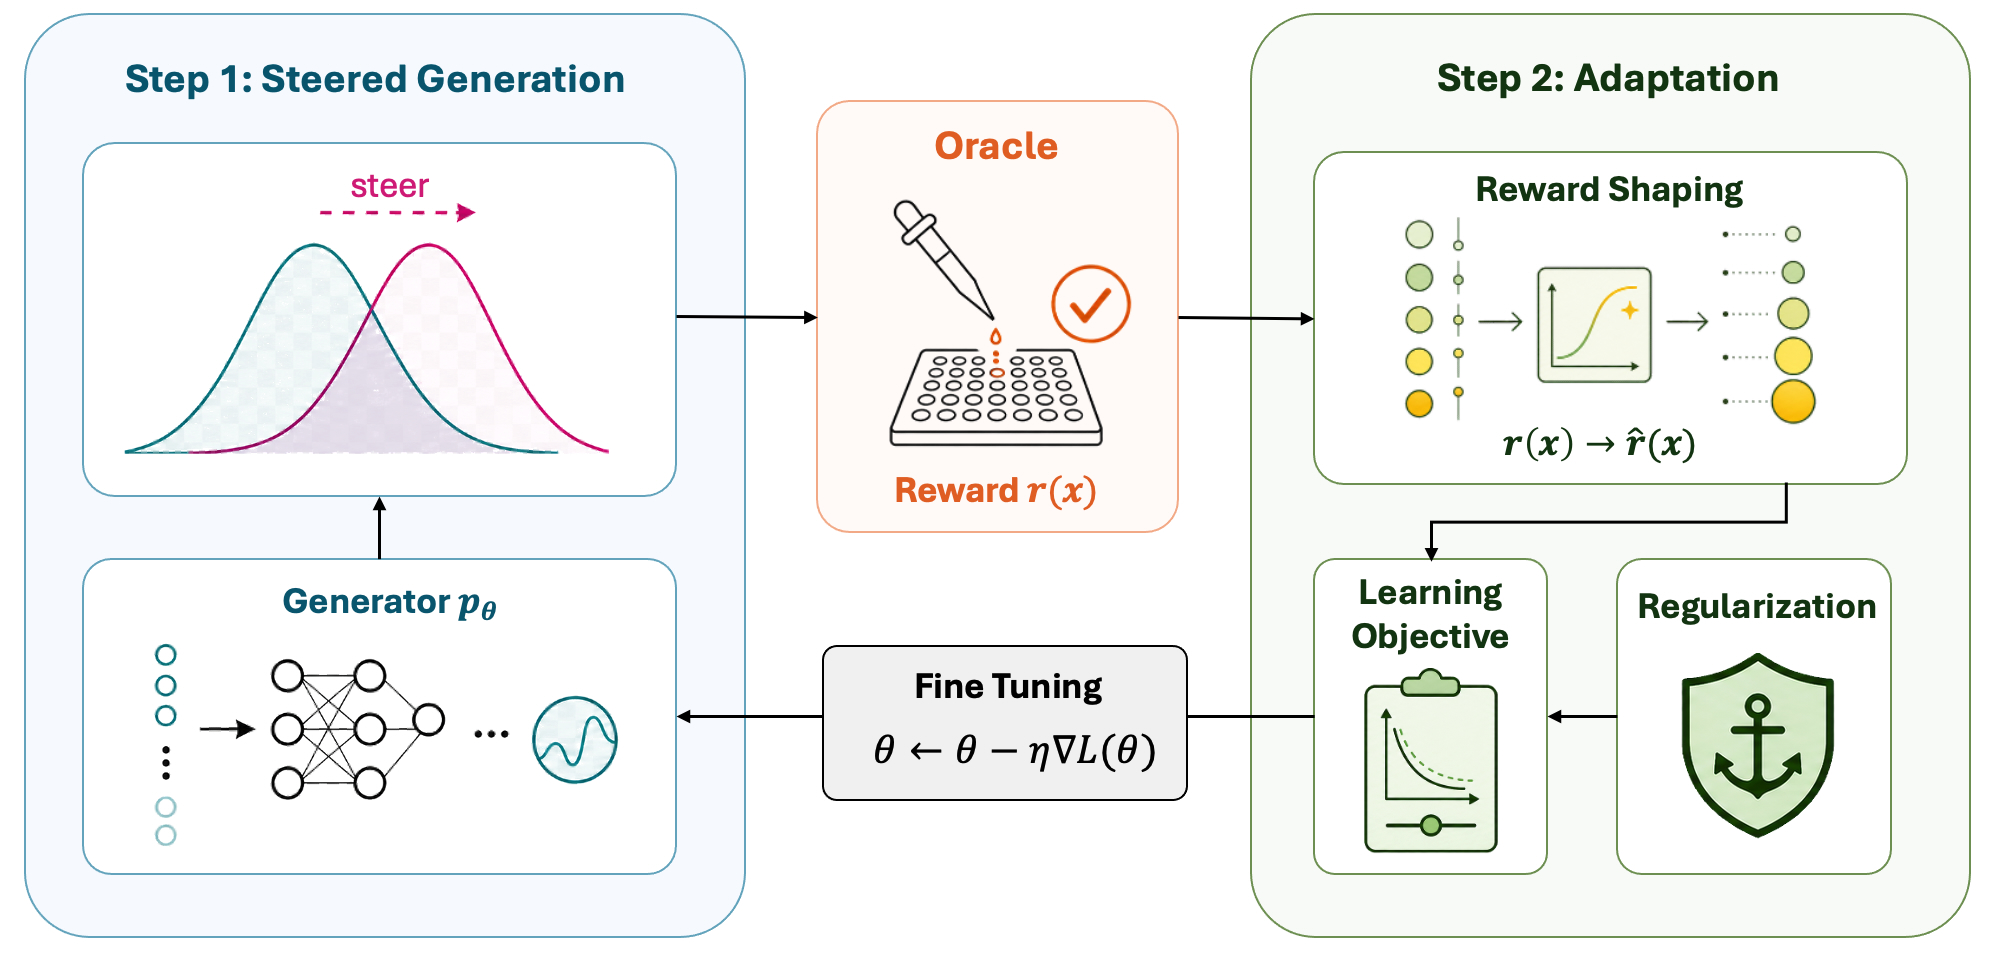
\includegraphics[width=\textwidth]{figures/overview.jpg}
    \vspace{-0.2in}
      \caption{\textbf{Online feedback loop for molecular optimization.}
Each round consists of two steps:
(1) the current generator $p_{\theta_t}$, updated using oracle feedback in Step~(2) of the previous round, generates candidates for the current round;
(2) the observed oracle rewards are converted into training signals to update the generator from $p_{\theta_t}$ to $p_{\theta_{t+1}}$.
The updated generator then returns to Step~(1), closing the online feedback loop.}
  \label{fig:test_time_feedback}
  \vspace{-0.1in}
\end{figure}


Our experiments on 9 tasks spanning small-molecule binding-affinity and protein-fitness optimization show that these mechanisms provide complementary benefits, especially when high-reward candidates have low likelihood under the pretrained generative prior. 
%In particular, density entropy regularization acts as model debiasing: it improves exploration even when acquisition already uses reward-model uncertainty, indicating that reward uncertainty and prior bias are distinct bottlenecks. Reward shaping, replay, and validity control likewise act on different parts of the loop: focusing updates on high-reward candidates, stabilizing learning over past feedback, and keeping exploration on the valid molecular manifold
On small molecules, acquisition, CVaR reward shaping, and Density Entropy Regularization provide the clearest complementary gains. On protein-fitness tasks, ablation effects are weaker, consistent with family-specific priors already covering high-fitness regions. Replay and validity control are primarily for keeping useful feedback across rounds and preventing exploratory updates from leaving the valid molecular manifold. 

\textbf{Overall, our contributions are: }
\begin{itemize}
    % \item We formulate test-time molecular optimization as an online feedback-allocation problem, where a fixed budget must be divided across candidate evaluation, reward modeling, replay, reward shaping, and generator updates.
    \item We provide a controlled empirical study of discrete-diffusion online adaptation for molecular optimization alongside offline fine-tuning and inference-time-search methods under fixed oracle and runtime budgets.

    \item We characterize the interactions among simple \emph{plug-in components} added to the online optimization loop through thorough ablations and mechanistic analysis: DER, CVaR, and Thompson Sampling exhibit compounding interactions while replay and validity control address distinct failure modes.

    \item We identify prior--reward mismatch as a useful diagnostic for when these mechanisms provide the most benefit. Under these observations, we assemble an online active fine-tuning recipe that substantially improves feedback efficiency over baselines.
    
    %We combine the best configurations of these components into a single online active fine-tuning recipe that outperforms all baselines at small-molecule and protein optimization under matched oracle-call budgets. We also elucidate that performance improvements are greater for molecular design solutions that lie further out of distribution from the original generative prior.
\end{itemize}
% \section{Introduction}
%Try to follow:

%- molecular optimization via discrete diffusion

%- unconditional gen. is not enough. we care about task-relevant designs hence use test-time training, where we can adapt the generative model via online feedback

%- problem: online feedback is very expensive

%- research question: how to optimally query and use costly online feedback for TT training?

%- We consider several important design choices of this process (exploration, objective missmatch etc. see slack -- present clearly \textbf{what they do intuitively}) and analyse them rigorously.

%- Results..

Discrete diffusion models have become a powerful tool for molecular generation, such as for small molecules \citep{leeGenMolDrugDiscovery2025, schiffSimpleGuidanceMechanisms2025} and proteins \citep{wangDiffusionLanguageModels2024}, because they can model realistic chemical structures directly while producing diverse candidate molecules. 
In molecular design, however, unconditional generation is rarely the final goal. 
A pretrained generator encodes a broad molecular prior whose probability mass is biased toward the pretraining distribution, while the design task defines a different target: molecules that score highly under a task-specific oracle. The generator must therefore be steered toward task-relevant regions of chemical space without losing the molecular validity that made the pretrained prior useful in the first place \citep{HowArtificialIntelligence,  ueharaInferenceTimeAlignmentDiffusion2025}.
A common way to do so is test-time adaptation, where one iteratively samples molecules, evaluates a small subset with a task oracle, and uses the feedback to steer future generations \citep{yangSteeringGenerativeModels2025, stoccoGuidingGenerativeModels2025}.
%A pretrained generator must produce parseable SMILES corresponding to chemically valid molecues, and beyond that score well for a specific task: binding to a target, improving a protein fitness score, satisfying a docking pipeline, or eventually passing a wet-lab assay. A common way to specialize a generator to such a task is test-time adaptation: sample molecules, evaluate them with a task oracle, and use the feedback to steer future generations.
%A common way to do so is test-time adaptation: sample molecules, evaluate a small subset with a task oracle, and use the feedback to steer future generations.





%Molecular optimization using generative models \citep{HowArtificialIntelligence} is often bottlenecked by feedback. A generative model can propose many candidate molecules, but each candidate becomes useful only after it is scored by an oracle, such as a learned binding-affinity model \citep{jiangFlashAffinityBridgingAccuracySpeed}, a structure-prediction/docking pipeline \citep{passaro2025boltz2}, or ultimately a wet-lab assay. These oracles are often expensive, non-differentiable and noisy relative to sampling from the generator. As a result, the central test-time question is not only how good the pretrained generator is, but how to allocate a limited number of oracle calls and subsequent computation \citep{didi2026scaling}.


%One attractive but relatively underexplored direction is test-time training, or online fine-tuning, for generative molecule optimization \citep{rector-brooksSteeringMaskedDiscrete2024, suIterativeDistillationRewardGuided2025, ueharaRewardGuidedIterativeRefinement2025, yangSteeringGenerativeModels2025, stoccoGuidingGenerativeProtein2025, stoccoGuidingGenerativeModels2025}. Test-time training uses evaluated molecules to update the generator itself. This has a natural advantage when oracle calls are scarce: each evaluation can influence the distribution of future samples, rather than only the sample selected now. In this paper, we focus on online fine-tuning of discrete diffusion models and ask which additions make this feedback loop work best.

%The difficulty is that task feedback is often the bottleneck. A generator can sample many molecules cheaply, but it cannot determine which samples are task-relevant until some of them are evaluated by an oracle, such as a learned binding-affinity model \citep{jiangFlashAffinityBridgingAccuracySpeed}, a structure-prediction or docking pipeline \citep{passaro2025boltz2}, or a wet-lab assay. These evaluations can be expensive relative to sampling from the generator. As a result, the central test-time question is not only how strong the pretrained generator is, but how to allocate a limited number of oracle calls and subsequent computation \citep{didi2026scaling}. In this paper, we ask how the full online training loop should use costly oracle feedback when optimizing a discrete diffusion model at test time.

The difficulty with  test-time adaptation is that it leads to a coupled design problem. A generator can sample many molecules cheaply, but it cannot determine which samples are task-relevant until some are evaluated by an oracle, such as a learned binding-affinity model \citep{jiangFlashAffinityBridgingAccuracySpeed}, a structure-prediction or docking pipeline \citep{passaro2025boltz2}, or a wet-lab assay. These evaluations can be expensive relative to sampling from the generator, so each oracle call must serve two roles: selecting useful candidate molecules now and providing feedback that can improve future generations. A key question is therefore not only how strong the pretrained generator is, or which fine-tuning objective is used, but how to reason holistically about the full online training loop: how it should allocate, reuse, and transform a limited stream of oracle feedback \citep{didi2026scaling}.



%We study this question through online fine-tuning for discrete-diffusion molecular optimization. Starting from a pretrained generator, the optimizer repeatedly samples molecules, decides which candidates to evaluate, receives oracle scores, and updates the generator from the scored molecules. This loop creates a growing history of feedback, but it leaves two central design problems open. The first is exploration: the optimizer must both query informative molecules to learn the unknown reward landscape and generate diverse candidates beyond the model's current high-probability regions. The second is objective mismatch: the oracle rewards only task-relevant molecules, while likelihood-based fine-tuning can spend capacity modeling low-value or invalid samples. These problems determine how the loop should allocate oracle calls, reuse past feedback, shape rewards, encourage exploration, and preserve validity.
%We study this question through online fine-tuning for discrete-diffusion molecular optimization. Starting from a pretrained generator, the optimizer repeatedly samples molecules, decides which candidates to evaluate, receives oracle scores, and updates the generator from the scored molecules. This loop creates a growing history of feedback, but it leaves two central design problems open. The first is exploration: the optimizer must both query informative molecules to learn the unknown reward landscape and generate candidates beyond regions already favored by the diffusion prior. The second is objective mismatch: the oracle rewards only task-relevant molecules, while likelihood-based fine-tuning can spend capacity modeling low-value or invalid samples. These problems determine how the loop should allocate oracle calls, reuse past feedback, shape rewards, encourage exploration beyond the prior's dominant modes, and preserve validity.
We therefore perform an integrated study of online training loops for  molecular optimization using discrete diffusion. Prior work has studied the main ingredients of this loop, including inference-time search with a fixed generator \citep{didi2026scaling, wangFineTuningDiscreteDiffusion2024, singhalGeneralFrameworkInferencetime2025, liDerivativeFreeGuidanceContinuous2024, nisonoffUnlockingGuidanceDiscrete2025, gruverProteinDesignGuided2023,  xiongProteinGuideOntheflyProperty2026, luProVADAGenerationSubcellular2025, ueharaRewardGuidedIterativeRefinement2025, liDynamicSearchInferenceTime2025, jianGeneralBindingAffinity2026, yangHitLeadDiscovery, tangTR2D2TreeSearch2025, yangSteeringGenerativeModels2025}, online fine-tuning from scored samples \citep{rector-brooksSteeringMaskedDiscrete2024, suIterativeDistillationRewardGuided2025, ueharaRewardGuidedIterativeRefinement2025, yangSteeringGenerativeModels2025, stoccoGuidingGenerativeProtein2025, stoccoGuidingGenerativeModels2025, liCAGenMolConditionAwareDiffusion2026, olivecronaMolecularNovoDesign2017, blalockFunctionalAlignmentProtein2025}, and reward-guided diffusion objectives that turn oracle feedback into a training loss \citep{wangFineTuningDiscreteDiffusion2024, ueharaRewardGuidedIterativeRefinement2025, ueharaFeedbackEfficientOnline2024, santiFlowDensityControl, tangTR2D2TreeSearch2025, ueharaInferenceTimeAlignmentDiffusion2025}.  We ask how representative design choices around the objective interact: whether choices for acquisition, feedback reuse, reward shaping, prior debiasing, and validity control provide distinct value, reinforce one another, or become redundant once combined \needcite.

%These pressures motivate complementary feedback mechanisms. Reward-model uncertainty motivates acquisition rules that use uncertainty to decide which candidates receive expensive oracle evaluations. Bias in the generative prior motivates prior debiasing, which encourages exploration beyond regions already favored by the current generator. Best-design discovery motivates reward shaping before fine-tuning, so high-reward candidates exert more influence on the update. Feedback reuse motivates replay, so useful evaluated molecules are not discarded after one gradient step. Validity constraints motivate penalties that keep optimization from exploiting invalid strings. Rather than proposing a new core fine-tuning objective, we ask how these mechanisms interact around existing reward-guided diffusion objectives.

%We study design choices across the major stages of the loop: selecting candidates for oracle evaluation, reusing evaluated samples, shaping oracle scores before fine-tuning, encouraging the generator to move beyond regions already favored by its pretrained prior, and preserving validity under aggressive optimization. This framing lets us test whether mechanisms aimed at different pressures---reward-model uncertainty, generative-prior bias, best-design discovery, feedback retention, and validity---compose into a stronger online loop or merely duplicate one another.


%Online fine-tuning still leaves several choices open. After each batch is scored, the method must choose which new candidates are worth evaluating, which past candidates should remain in the training set, how much weight to put on the highest-scoring molecules, and how to keep the generator from producing invalid molecules. Emphasizing only the best molecules may improve top scores but reduce exploration. Pushing the model away from familiar regions may uncover new candidates but damage validity. Reusing past high-scoring molecules can stabilize learning, but may slow adaptation to new regions. This leaves an empirical question: which parts of the online loop matter most, do their benefits add or saturate, and how do they behave under shared oracle-call and runtime accounting?

%We turn these problems into a controlled study of the online feedback loop. To address statistical exploration, we use Thompson sampling (CITE) over a reward model so oracle calls target molecules that are both promising and uncertain. To address computational exploration, we add a model-debiasing term that discourages the generator from staying only in high probability regions of its current distribution. To align training with the optimization goal, we use a tail-focused objective that concentrates updates on high-scoring molecules. Because this pressure can push the generator toward invalid structures, we add an invalid-output penalty during fine-tuning. Finally, because oracle calls are costly, we maintain a replay buffer of evaluated molecules so useful feedback can influence multiple generator updates. We compare against offline fine-tuning to test whether feedback must be incorporated online, and against search-based variants to test whether additional inference-time exploration still helps once the generator itself is being updated.
Our experiments show that these mechanisms are complementary rather than redundant. In particular, likelihood-based debiasing improves exploration even when acquisition already accounts for reward-model uncertainty, suggesting that uncertainty in the reward model and bias in the generative prior are distinct bottlenecks. Reward shaping, replay, and validity control affect different parts of the training signal and failure profile rather than substituting for a stronger fine-tuning objective. Across 6 small-molecule binding-affinity and 3 protein fitness optimization tasks, the combined online training loop [RESULT] offline fine-tuning and search-augmented variants under matched oracle-call budgets, with [RESULT] under [GPU-hour / wall-clock] accounting.

%We study this question in discrete-diffusion molecular optimization by turning the online loop into a set of testable design choices. Starting from a pretrained generator, we repeatedly sample molecules, choose which ones receive oracle calls, store evaluated molecules for future updates, adjust their rewards, and fine-tune the generator. Each component targets one part of this loop. An exploration bonus on the reward model helps allocate oracle calls. A replay buffer retains useful feedback across updates. A tail-focused reward estimate makes learning less sensitive to low-value samples. A negative likelihood regularization term pushes the generator away from over-occupied regions, while an invalid-output penalty keeps fine-tuning near the valid molecular manifold. Offline fine-tuning and search-based variants serve as diagnostic baselines, testing whether feedback must be incorporated online and whether additional inference-time exploration still helps once the generator is being updated.

%Our experiments show that the main design choices are complementary rather than redundant: the strongest results require both forms of exploration, reward shaping, replay, and validity control. Each choice improves a different part of the online loop. Statistical exploration improves where oracle calls are spent, computational exploration expands the regions the generator reaches, reward shaping determines how scores become gradients, replay preserves useful feedback across updates, and validity control prevents reward optimization from producing invalid molecules. Ablating these choices reveals distinct failure modes rather than a single dominant component. Across [TASKS/TARGETS], the combined recipe [RESULT] offline fine-tuning and search-based variants under matched oracle-call budgets, with [RESULT] under [GPU-hour / wall-clock] accounting.

Our contributions are:
\begin{itemize}
    \item We formulate test-time molecular optimization as an online feedback-allocation problem, where a fixed budget must be divided across candidate evaluation, reward modeling, replay, reward shaping, and generator updates.

    \item We provide a controlled study of online fine-tuning for discrete-diffusion molecular optimization under oracle-call and runtime accounting, with offline fine-tuning and search-based variants included as diagnostic baselines.

    \item We show that several simple additions to the online loop provide complementary benefits: Thompson sampling over the reward model improves oracle-call allocation, replay stabilizes learning, CVaR reward shaping focuses updates on high-reward candidates, model debiasing encourages exploration beyond dominant modes, and invalid-output penalties preserve molecular validity.

    \item We combine these components into a single online active fine-tuning recipe that [RESULT] across [TASKS/TARGETS] under matched oracle-call budgets, with [RESULT] under [GPU-hour / wall-clock] accounting.
\end{itemize}
% \section{Problem Setup}
\label{sec:problem-setup}


Molecular optimization at test time is an online decision-making problem: given a pretrained generator $p_{\theta_0}$, a task oracle $r(x)$, and a finite evaluation budget $B$, the goal is to maximize a discovery utility $U(\mathcal{D}_B)$ over the set of evaluated molecules $\mathcal{D}_B$. In the simplest case, $$U(\mathcal{D}_B)=\max_{x\in\mathcal{D}_B} r(x)$$
is the best molecule discovered; other choices can measure the top-$k$ mean or the quality of the upper tail. The loop in Fig.~\ref{fig:test_time_feedback} operationalizes this objective. At round $t$, the current discrete diffusion generator $p_{\theta_t}$ samples a candidate pool $C_t=\{x_i\}_{i=1}^M$. The loop selects a smaller set $S_t\subset C_t$ of $K$ candidates for oracle evaluation, appends the scored pairs to the evaluated set $\mathcal{D}_{t+1}=\mathcal{D}_t\cup\{(x,r(x)):x\in S_t\}$, and stops when $|\mathcal{D}_t|=B$.
Each round alternates between two high-level steps.  The first step samples candidates from $p_{\theta_t}$, optionally steers generation using a reward surrogate, and selects candidates for oracle evaluation. The second step transforms the resulting scores into training signal and updates the generator to $p_{\theta_{t+1}}$ before the next round. %Oracle feedback therefore has two coupled roles: it determines the current discovery utility and supplies data that changes which candidates the loop will propose later.

\textbf{Step 1: Steered Generation with Diffusion Prior.}
The loop begins with a pretrained discrete diffusion model $p_{\theta_0}$ that serves as the molecular prior over candidate sequences $x$, such as SAFE strings for small molecules or amino-acid sequences for proteins. Sampling from $p_{\theta_t}$ means running the model's denoising dynamics to completion and returning candidate molecules. In the online loop, the current generator $p_{\theta_t}$ is both the source of new candidates and the model being updated from feedback.

Because oracle evaluations are expensive relative to sampling, the loop cannot score every generated candidate. It must decide which candidates receive oracle calls. This selection step can use a learned reward surrogate, uncertainty estimates, or inference-time search to steer generation or prioritize candidates. These mechanisms determine where the loop spends its evaluation budget, but by themselves they do not determine how feedback changes the generator.

\textbf{Step 2: Reward Shaping \& Fine-Tuning.}
Each selected candidate is scored by a task oracle $r(x)$, such as a binding-affinity predictor, docking pipeline, structure-prediction model, or wet-lab assay. The raw score is not necessarily the signal used for training. The loop may reshape rewards to emphasize the upper tail, penalize invalid molecules, or encourage exploration beyond regions already favored by the current generator. One useful diagnostic is the generator's denoising log-likelihood $\log p_{\theta_t}(x)$: high likelihood means that $x$ lies in a region the current generator already covers well, while low likelihood indicates a less occupied region of the model distribution. Section~\ref{sec:design-space} uses this quantity for model debiasing.

After oracle evaluation, the loop updates the generator using evaluated pairs $(x,r(x))$. A fine-tuning objective specifies how scored samples become gradients, but it does not by itself specify the full online algorithm. The loop must also decide whether to train only on the latest batch or replay past evaluated molecules, how much fresh feedback to mix with retained high-reward samples, and how to prevent reward optimization from leaving the valid molecular manifold.


%This paper studies the design space induced by the loop in Fig.~\ref{fig:test_time_feedback}. The central issue is not only which fine-tuning objective is used, but how the loop allocates oracle calls, reuses feedback, shapes rewards, explores beyond the current generator's dominant modes, and preserves validity. The next section turns these decisions into modular design choices that can be ablated independently.


\section{Plug-In Components of Online Adaptation} 
\label{sec:design-space}

We frame the loop in Fig.~\ref{fig:test_time_feedback} as a \emph{harness}: a fixed online schedule with swappable components at the points where feedback is collected, transformed, and used for fine-tuning. Each round generates candidates, selects a subset for oracle evaluation, converts oracle scores into training rewards, regularizes the update, and fine-tunes the generator. As a \emph{harness}, it is finetuner-agnostic and domain-agnostic: any discrete generator with objective $\mathcal{L}_{\text{ft}}$ that consumes per-sample log-rewards and an off-policy buffer can be used; we instantiate it with DDPP-LB~\citep{rector-brooksSteeringMaskedDiscrete2024} and VIDD~\citep{suIterativeDistillationRewardGuided2025}.

We organize the components by their role in the feedback loop. \emph{Steering strategies} affect which candidates receive oracle evaluations (Sec.~\ref{sec:design-explore}); \emph{adaptation strategies} determine how observed rewards shape the model update (Sec.~\ref{sec:adaptation_design}); and \emph{objective-mismatch corrections} keep optimization aligned with accumulated feedback and valid molecules as exploration shifts the sampling distribution $p_{\theta_t}$ (Sec.~\ref{sec:design-objmismatch}). For each category, we instantiate one representative choice adapted from prior work (Table~\ref{tab:methods}). The per-knob ablations in Sec.~\ref{sec:results} then test whether these choices retain distinct value when composed.

\begin{table}[h]
\centering
\small
    \begin{tabular}{@{}p{4.4cm}p{9.3cm}@{}}
\toprule
\textbf{Knob} & \textbf{Description} \\
\midrule
$+$ CVaR~\citep{santiFlowDensityControl, wang2026efficient}            & Replace $r$ with $(r - Q_\tau)_+/(1-\tau)$, $\tau{=}0.8$ \\
$+$ Density Entropy Reg.~\citep{de2025provable}  & Add $-\gamma \log p_\theta(x)$ to log-reward, $\gamma{=}1$ \\
$+$ Thompson~\citep{thompson1933likelihood, chapelle2011empirical}        & $J{=}10$ MLP ensemble; oracle top-$K$ by $s_i \sim \mathcal{N}(\mu_i, \sigma_i^2)$ \\
$+$ Replay buffer~\citep{mnih2015human}   & Fixed-capacity FIFO with priority eviction; stratified sampling \\
$+$ Invalid penalty~\citep{wangFineTuningDiscreteDiffusion2024, ueharaELEGANT2024}  & Assign $r {=} r_{\text{inv}}$ to SMILES that fail RDKit parsing \\
\bottomrule
\end{tabular}
\caption{\textbf{\emph{Harness} knobs: plug-in components evaluated in this paper.} Each knob layers on top of finetuner and is ablated independently in Section~\ref{sec:results}, then evaluated jointly in the final recipe of Sec.~\ref{sec:results-method}.}
\label{tab:methods}
\vspace{-0.2in}
\end{table}



\subsection{Steering Strategies}\label{sec:design-explore}

%\begin{figure}[b]
%  \centering
%  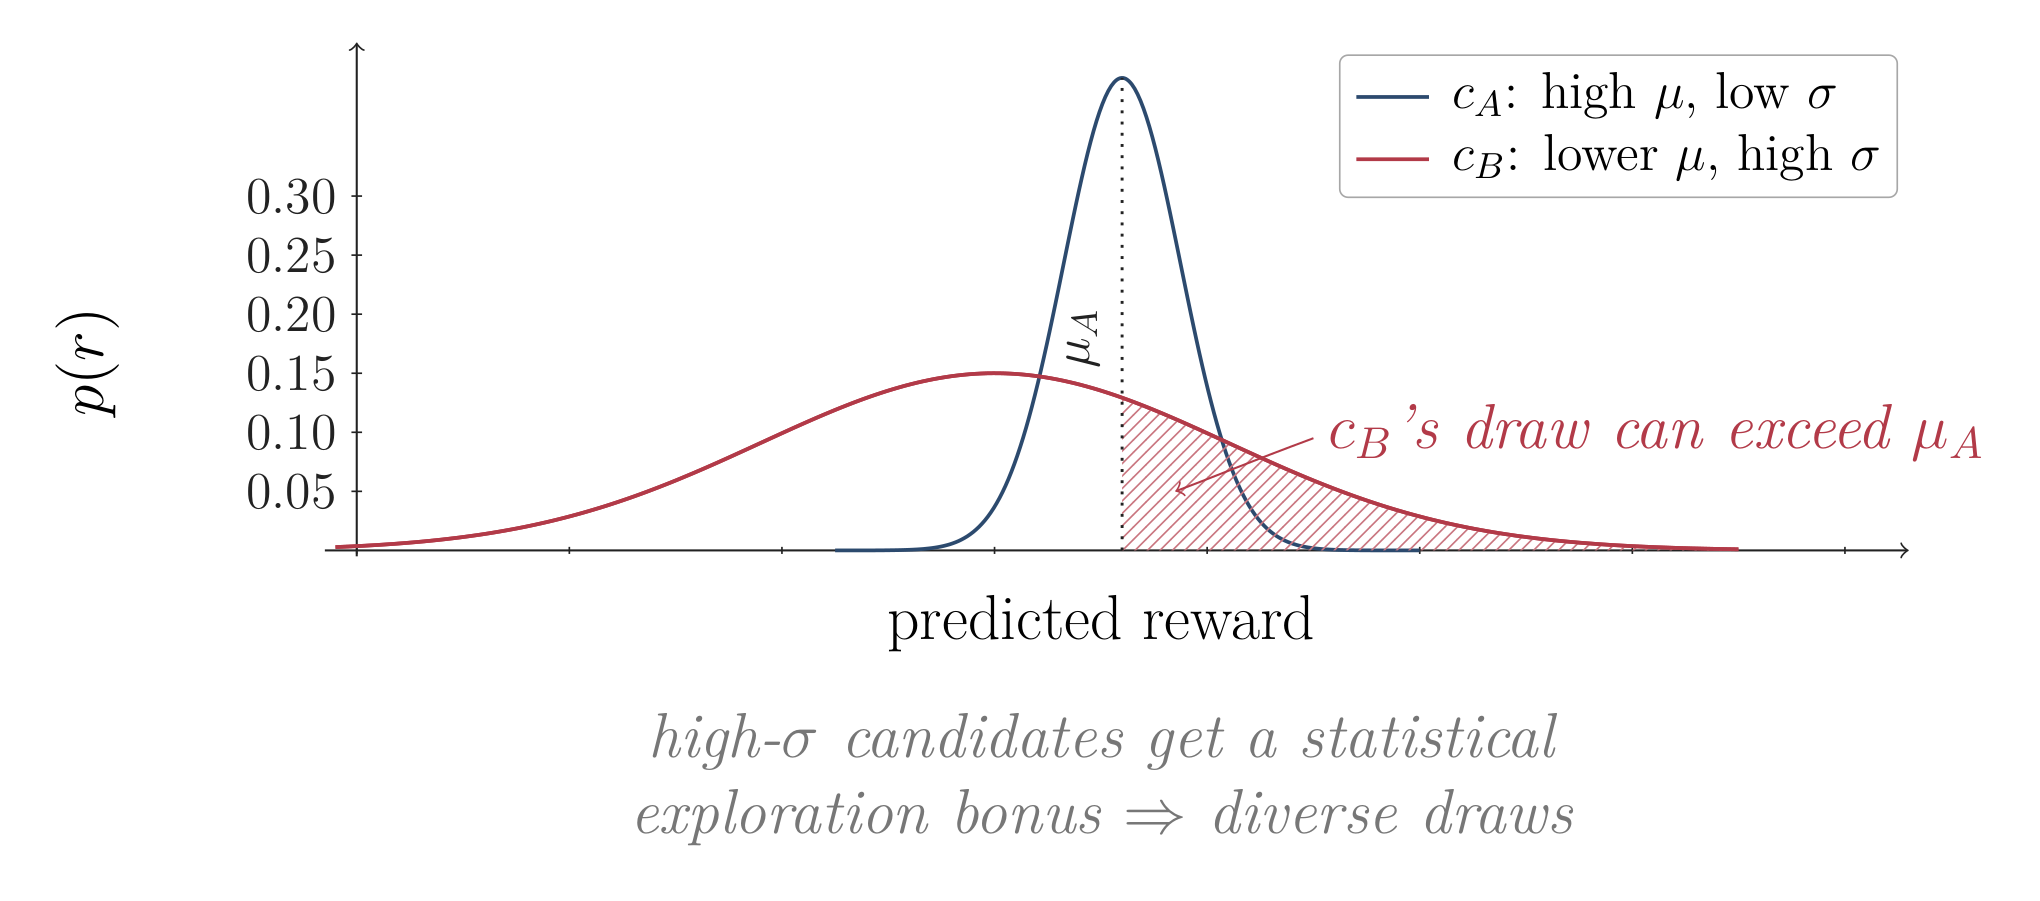
\includegraphics[width=0.65\textwidth]{figures/diagram_thompson.png}
  %\vspace{-0.15in}
  %\caption{\textbf{Thompson sampling.} Two candidates' %ensemble posteriors over predicted reward: $c_A$ (low %$\sigma$, greedy pick at $\mu_A$) and $c_B$ (lower mean, higher $\sigma$). Hatched area $= \Pr[\hat r_B > \mu_A]$ is the probability that $c_B$'s Thompson draw exceeds the deterministic-greedy threshold.}
  %\label{fig:diag_thompson_body}
%\end{figure}
\begin{figure}[b]
  \centering
  \begin{minipage}[t]{0.64\textwidth}
    \vspace{0pt}
    \centering
    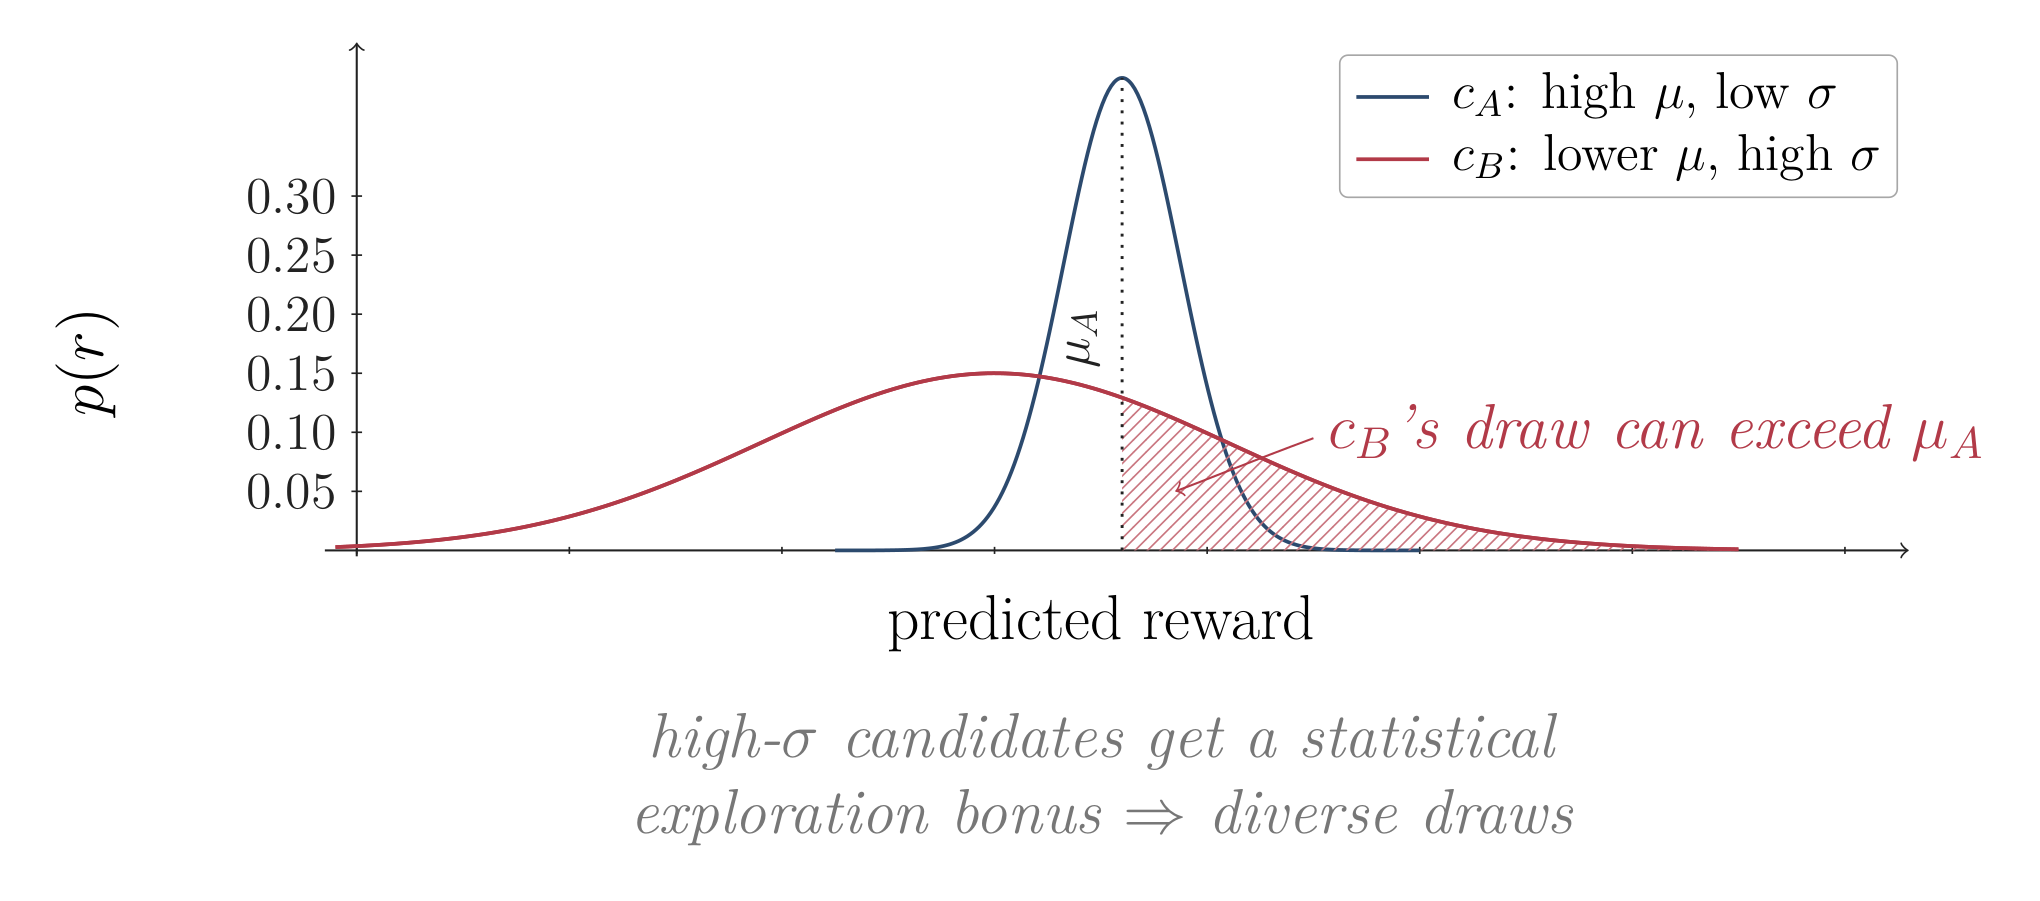
\includegraphics[width=\linewidth]{figures/diagram_thompson.png}
  \end{minipage}
  \hfill
  \begin{minipage}[t]{0.35\textwidth}
    \vspace{0pt}
    \caption{\textbf{Thompson sampling.} Although $c_A$ has the higher mean prediction, $c_B$ can be selected because its larger uncertainty gives it nonzero probability of drawing above the greedy threshold.}
    \label{fig:diag_thompson_body}
  \end{minipage}
\end{figure}


\textbf{Thompson Sampling Acquisition.} Because the oracle budget is finite, the loop must choose a small subset of generated candidates for evaluation. The simplest rule evaluates the candidates with the highest predicted reward under a surrogate model. This greedy rule is purely exploitative: it spends oracle calls where the surrogate already predicts high reward. We also consider uncertainty-aware acquisition using Thompson sampling \citep{thompson1933likelihood, russo2018tutorial}. Given an ensemble surrogate with mean $\mu_i$ and disagreement $\sigma_i$ for candidate $x_i\in C_t$, Thompson sampling draws a sampled reward estimate:
\[
\hat r_i = \mu_i + \varepsilon_i \sigma_i, \qquad \varepsilon_i \sim \mathcal{N}(0,1),
\]
and evaluates the top-$K$ candidates by $\hat r_i$, defining the selected batch $S_t$. Fig.~\ref{fig:diag_thompson_body} depicts the intuition behind how Thompson sampling balances the explore/exploit trade-off.  Candidates with high uncertainty can outrank candidates with higher predicted mean but lower uncertainty, i.e., this scheme incentivizes to explore seemingly lower quality but high uncertainty candidates. %This uses oracle calls to reduce uncertainty in promising regions rather than only confirming the surrogate's current maximum.


% The contrast with deterministic top-$\mu$ selection is sharp (Fig.~\ref{fig:diag_thompson_body}): under deterministic selection a candidate $c_B$ with $\mu_B < \mu_A$ never gets oracle-evaluated, no matter how uncertain it is, so the training data $(x, r(x))$ that downstream finetuning sees is concentrated on the current surrogate argmax. As the ensemble disagreement $\sigma_B$ grows away from zero, the Thompson rule smoothly transitions from this hard-greedy regime to a stochastic exploration bonus, the standard way to guard against local optima \citep{chapelle2011empirical}. The acquisition step is itself modifying which samples from $p_{\theta_t}$ enter the evaluated set and therefore which data the gradient computes against. A fuller comparison against deterministic top-$\mu$ selection is given in Appendix~\ref{app:knob-interactions}.




%\begin{figure}[t]
%  \centering
%  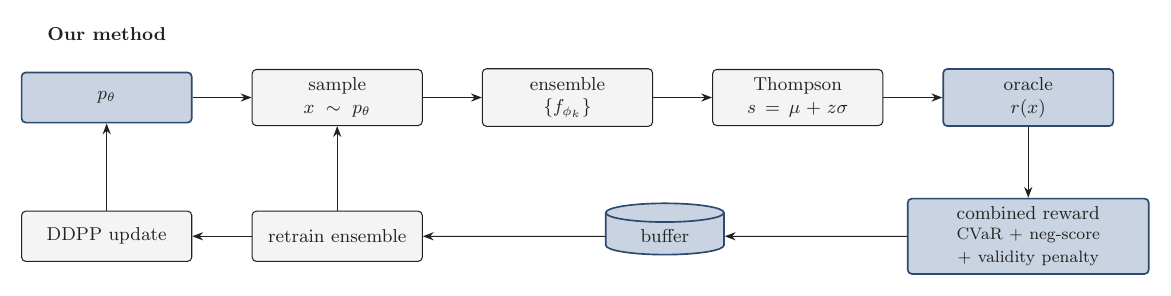
\includegraphics[width=0.95\textwidth]{figures/diagram_final.png}
%  \caption{\textbf{Online active loop.} Schematic of the composable-knob harness evaluated in this paper. Each round samples $M$ candidates from $p_{\theta_t}$, scores them under the surrogate ensemble, oracle-evaluates the Thompson-selected top-$K$ (with invalid candidates assigned $r_{\text{inv}}$ before they reach the oracle), pushes the resulting $(x, r)$ pairs to the buffer, and updates $p_{\theta_t}$ to $p_{\theta_{t+1}}$ via DDPP-LB on the CVaR + debiasing-shaped log-reward; the ensemble is refit on the buffer at the end of each round. Pseudocode in Appendix~\ref{app:diagrams}, Algorithm~\ref{alg:method}.}
%  \label{fig:diag_final}
%\end{figure}

\subsection{Adaptation Strategies}\label{sec:adaptation_design}

\textbf{CVaR-Style Reward Shaping.}
\looseness -1 A second lever acts on the reward itself after oracle evaluation and before it enters the gradient. We write the resulting shaped training reward as $\tilde r(x)$. Because the design objective in Eq. \eqref{eq:design_objective} is controlled by the upper tail rather than the average generated molecule, we adapt the model via a CVaR-style \citep{rockafellar2000cvar, rockafellar2002cvar} objective (Fig.~\ref{fig:diag_reward_shaping}(a)), as introduced in prior work on diffusion model adaptation~\citep{santiFlowDensityControl, wang2026efficient}. This objective allows to sacrifice the average sample reward to enhance the quality of top-samples:
\[
\mathrm{CVaR}_{1-\tau}[r(x)]
=
\mathbb{E}\!\left[
r(x) \mid r(x) \ge Q_\tau(r)
\right].
\]
% Upper-tail shaping alone can still repeatedly reinforce regions the generator already samples frequently, so we add a score-based debiasing term:
% \[
% \log \tilde r_{\mathrm{debias}}(x)
% =
% \log \tilde r_{\mathrm{cvar}}(x) - \gamma \log p_{\theta_t}(x),
% \]
% where $\log p_{\theta_t}(x)$ denotes the model likelihood term used inside the discrete diffusion training dynamics. At the loop level, $x$ is a candidate molecule; inside the denoising loss, the same notation may refer to the corresponding noised or partially denoised state. The value is treated as a constant for gradient purposes. This favors candidates that are high reward but not already high likelihood under the current generator.

\begin{figure}[htbp]
  \centering
  \begin{minipage}[c]{0.49\textwidth}\centering
    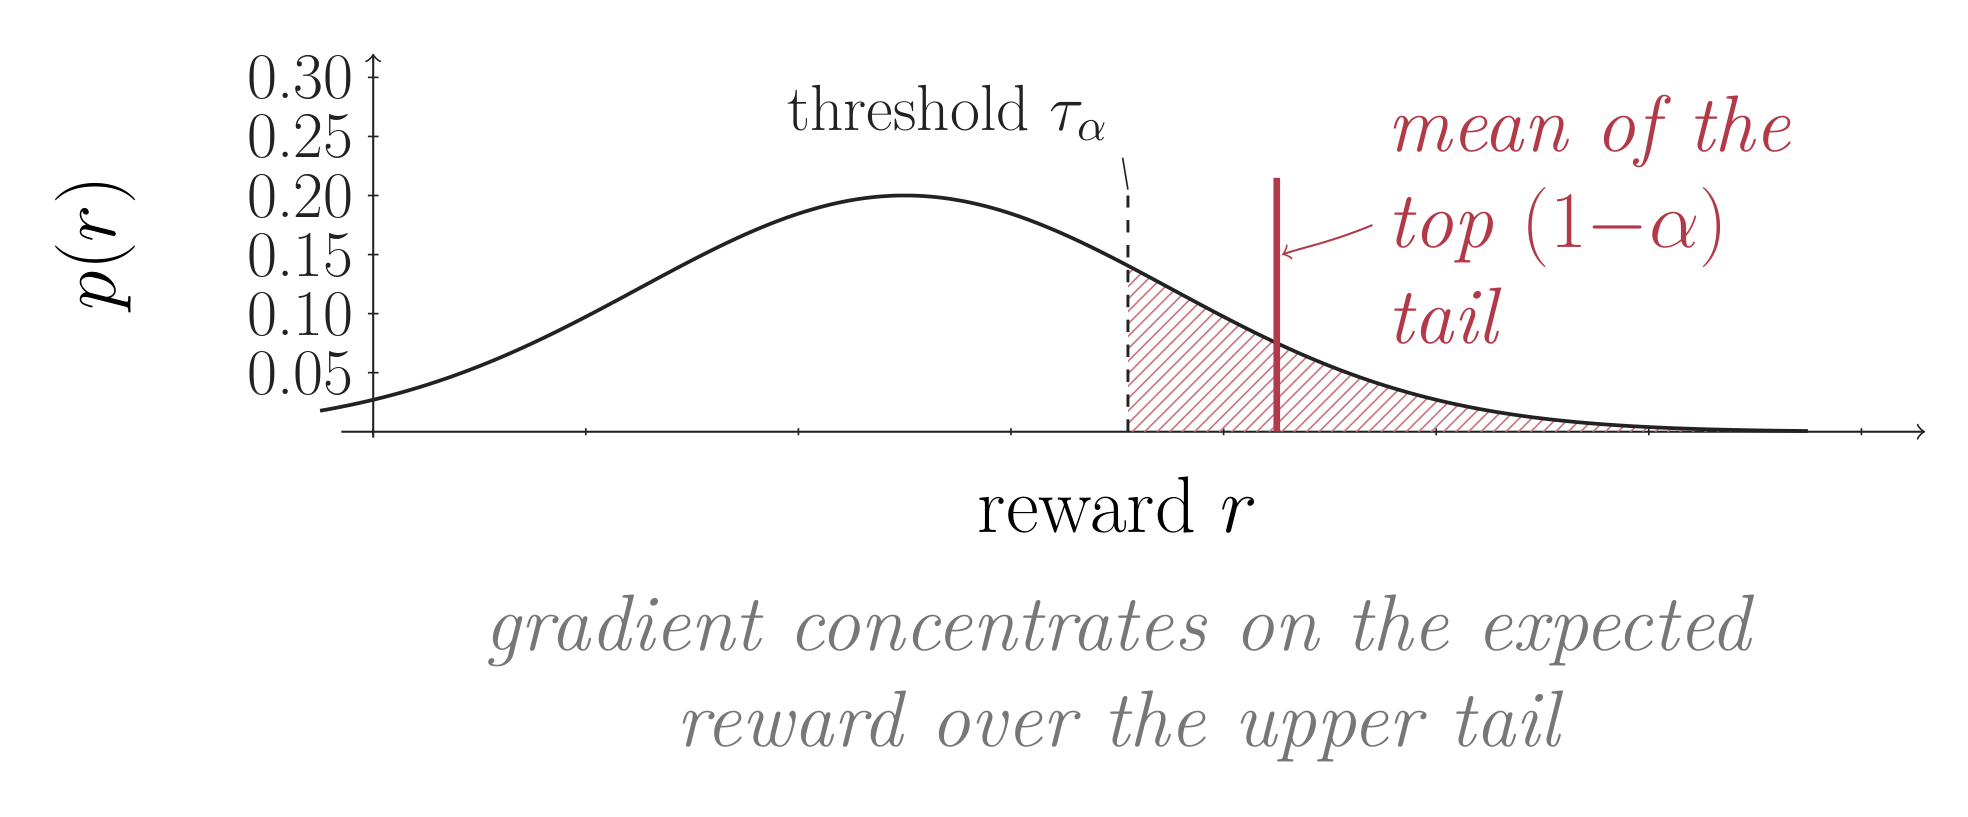
\includegraphics[width=\textwidth]{figures/diagram_cvar.png}\\
    \textbf{(a)} CVaR Shaping
  \end{minipage}\hfill
  \begin{minipage}[c]{0.49\textwidth}\centering
    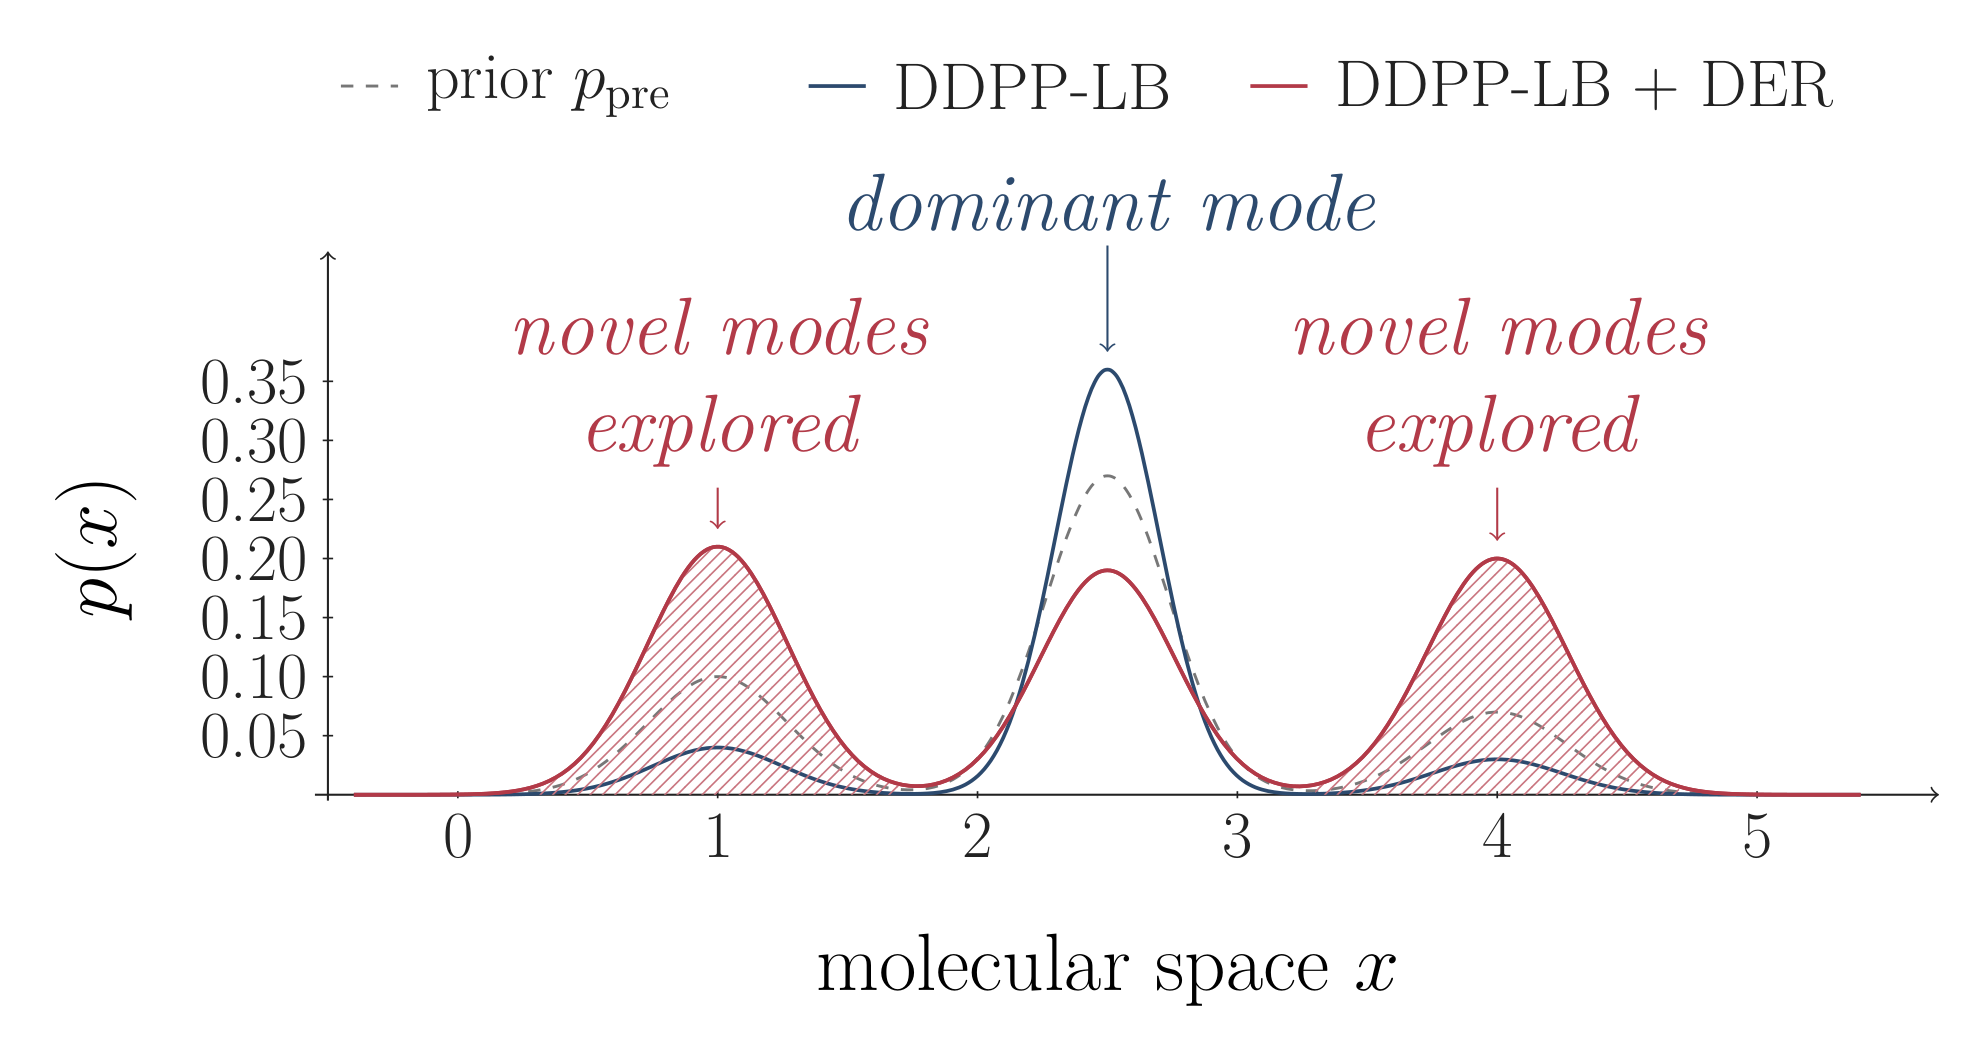
\includegraphics[width=\textwidth]{figures/diagram_debiasing.png}\\
    \textbf{(b)} Density Entropy Regularization
  \end{minipage}
  \caption{\textbf{Reward-shaping and model debiasing} \textbf{(a)} CVaR upper-tail shaping: the right-tail of the reward distribution above the $\tau$-quantile (dashed) is shaded, and the solid red bar marks $\mathrm{CVaR}_{1-\tau} = \mathbb{E}[r \mid r \geq Q_\tau]$, the expected reward conditional on being in that tail. Optimization concentrates gradient on this tail expectation, not on a hard top-$k$ selection. \textbf{(b)} Density Entropy Regularization (model debiasing): subtracting the current generator's diffusion-internal likelihood $\log p_{\theta_t}(x)$ from the log-reward redistributes gradient mass off densely-occupied modes and toward less-frequented regions, exposing minor modes the unshaped reward would have kept under-explored.}
  \label{fig:diag_reward_shaping}
  \label{fig:diag_cvar_body}
  \label{fig:diag_debiasing_body}
\end{figure}

\textbf{Density Entropy Regularization.}
CVaR reward shaping focuses the update on the upper tail, but it does not distinguish between high-reward regions that the generator already samples frequently and high-reward regions that remain underexplored. To expose this distinction independently of CVaR, practitioners can apply a density-entropy regularizer~\citep{de2025provable, santiFlowDensityControl, santiVerifierConstrainedFlowExpansion2026} that uses the current model density as a measure of how occupied a region is under the generator and shapes the raw log-reward as:
\begin{equation}
\log \tilde r_{\mathrm{debias}}(x)
=
\log r(x) - \gamma \log p_{\theta_t}(x),
\label{eq:debias}
\end{equation}
illustrated in Fig.~\ref{fig:diag_reward_shaping}(b), where $\log p_{\theta_t}(x)$ is the marginal. In continuous-diffusion analyses~\citep{de2025provable, santiFlowDensityControl}, the corresponding negative-score gradient $\nabla_x \log p_{\theta_t}(x)$ can be directly approximated by the available score network,  but in masked discrete diffusion it is estimated by the marginalization:
\[
p_{\theta_t}(x_0) \;=\; \mathbb{E}_{t, \, x_t \sim q(x_t \mid x_0)}\!\bigl[\,p_{\theta_t}(x_0 \mid x_t)\,\bigr] \cdot \text{(noise-schedule weight)},
\]
a sum over an exponentially-large set of noised states $x_t$, making it intractable. For discrete diffusion the proper asymptotic unbiased estimator is a Monte-Carlo ELBO \citep{nie2025llada} (LLaDA, Algorithm~3), which costs $n_{\text{mc}}$ extra forward passes per evaluation.

We replace $\log p_{\theta_t}(x)$ in Eq.~\ref{eq:debias} with the cheapest such estimator: 
\[
\widehat{\log p_{\theta_t}(x)} \;\equiv\; \log p_{\theta_t}(x_0 \mid x_t)
\;=\;
\textstyle\sum_{i \,:\, x_t^i = [\text{MASK}]}\, \log \mathrm{softmax}(\ell_i)\bigl[x_0^i\bigr].
\]
This estimator is a cheap approximation of the diffusion ELBO, so it is not equivalent to the MCMC-estimated continuous negative-score regularizer or to the LLaDA-style $L/l$-weighted estimator in the limit. We choose this estimator  for computational reasons: the alternatives cost $n_{\text{mc}}\!\times$ extra forward passes per gradient step, which is prohibitive across thousands of online finetuning steps. Despite the approximation, we find empirically that it induces the intended distribution shift and that the added noise leads to more exploration and overall better performance. we find empirically that it achieves comparable oracle-call efficiency to LLaDA-Alg.\,3 variants with $n_{\text{mc}} \in \{1, 4, 8, 16\}$ while being substantially faster per GPU hour. Post-hoc evaluation with the unbiased LLaDA-Alg.\,3 estimator ($n_{\text{mc}}{=}32$) confirms that the resulting NLL distributions from the cheap estimator follows closely to the LLaDA estimator with wider exploration (Appendix Figs.~\ref{fig:negscore_estimator_curves} and~\ref{fig:negscore_nll_dist}).
Intuitively, this term favors candidates that are high reward but not already high likelihood under the generator, complementing Thompson-sampling acquisition (acquisition vs.\ reward-shape act on the loop at different points; see Appendix~\ref{app:knob-interactions} and Fig.~\ref{fig:diag_debiasing_body}).
The estimated value is detached, so the parameter gradient enters the standard DDPP-LB / VIDD policy-gradient term as a scalar reward modifier  (Appendix~\ref{app:method-details}).


\subsection{Objective-mismatch corrections}\label{sec:design-objmismatch}

Once exploration starts shifting $p_{\theta_t}$ off the prior's dominant modes, two gaps open between what the gradient actually optimizes and the true objective. The next two components can close them.

\textbf{Replay Buffer.}
A remaining choice is which evaluated samples appear in each update. A purely on-policy update trains only on the latest batch, so useful molecules discovered early stop influencing the generator once the sampling distribution moves on. We therefore optionally train from a replay buffer that mixes fresh candidates with retained high-reward samples \citep{mnih2015human, schaul2016prioritized, olivecronaMolecularNovoDesign2017}. Concretely, the buffer is fixed-capacity FIFO with priority eviction (when full, the lowest-reward sample leaves first, not the oldest), and each minibatch is drawn by stratified sampling across reward bins so high-reward outliers don't get diluted by a larger volume of mid-reward fresh candidates.

\textbf{Invalid-output penalty.}
To keep optimization on the molecular manifold, candidates that fail validity checks, ie RDKit parsing \citep{rdkit} in the case of small molecules, receive a fixed penalty $r_{\mathrm{inv}}<0$ and enter training as low-reward examples. The mismatch this corrects is between the oracle's reward (defined for any string) and the actual objective (high reward on a valid molecule); the penalty closes that gap by giving the gradient an explicit signal to pull $p_{\theta_t}$ back toward the valid molecular manifold.



\section{Experimental Setup}
\label{sec:experimental-setup}\label{sec:exp-setup}

\begin{figure}[htbp]
  \centering
  \vspace{-0.1in}
  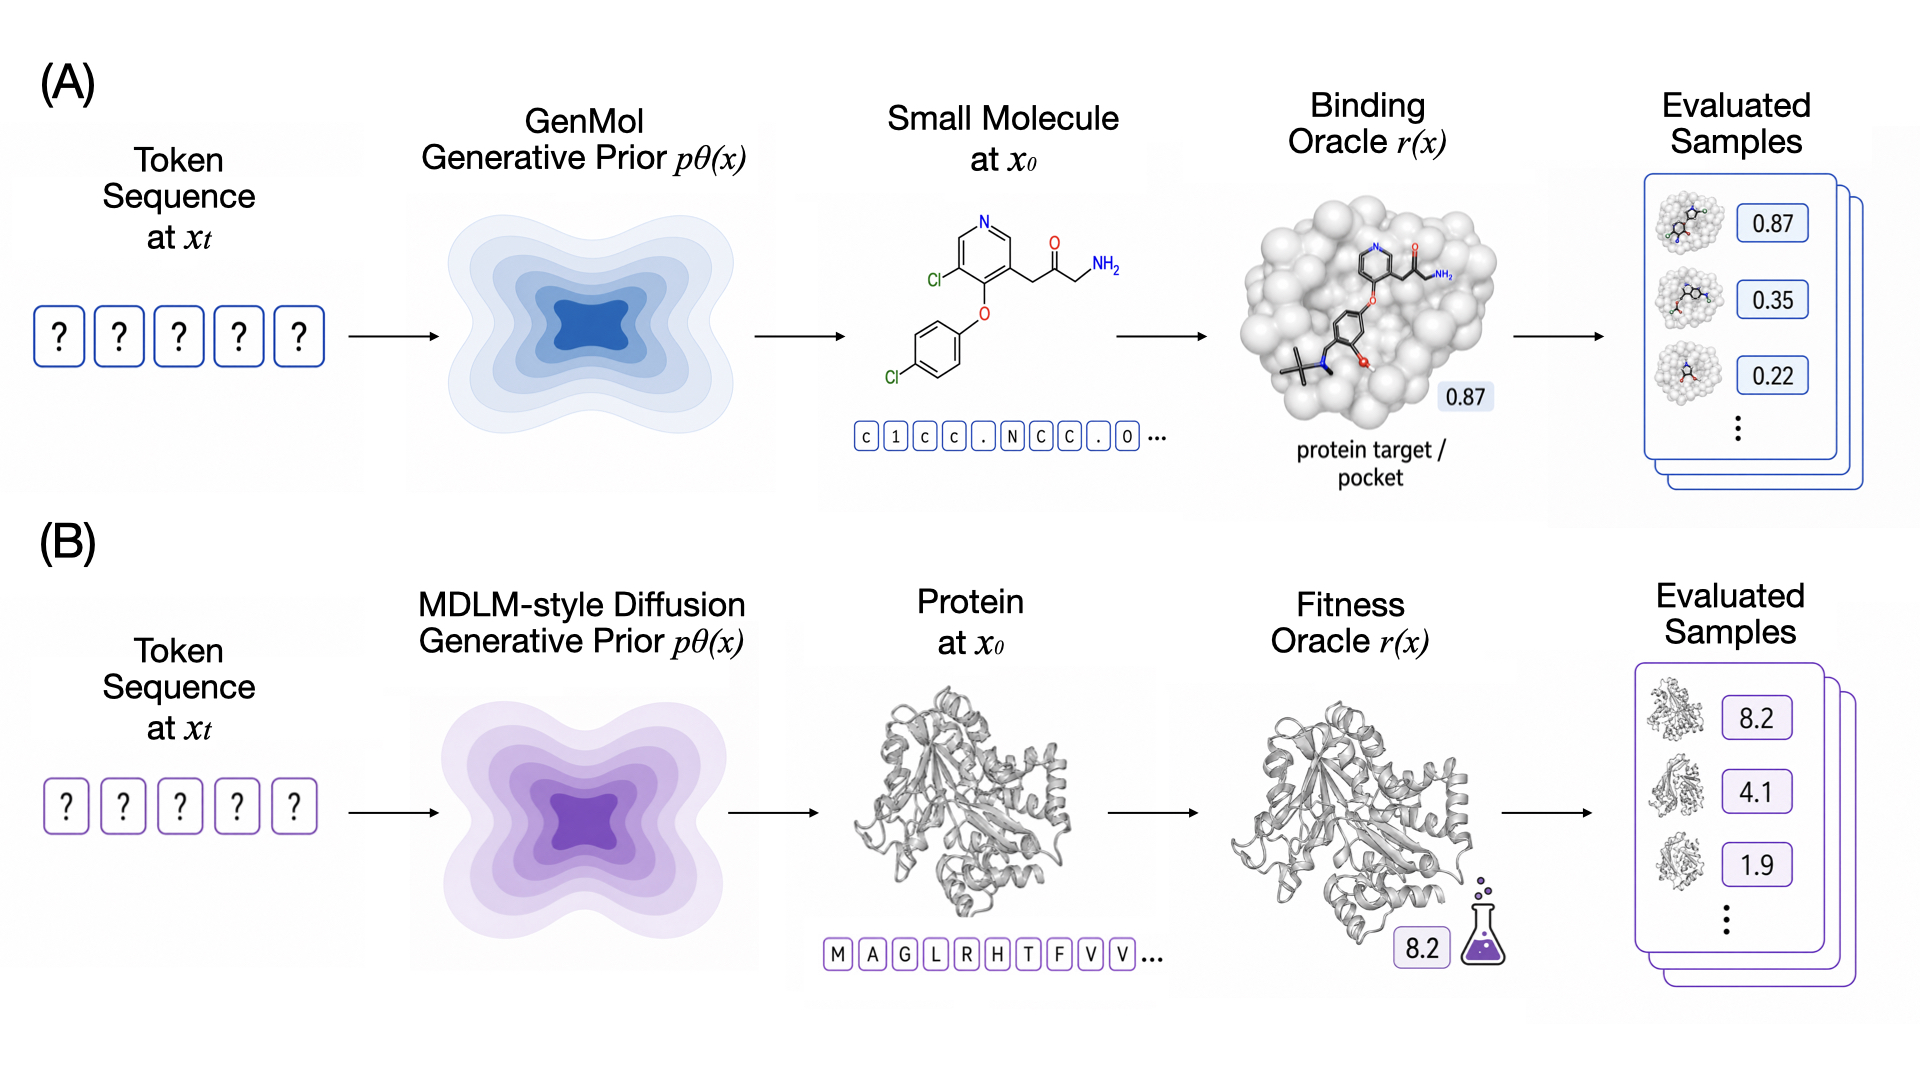
\includegraphics[width=\textwidth]{figures_source/Applications002.jpeg}
  \vspace{-0.4in}
  \caption{In this study, we explore several tasks across two different domains, optimizing \textbf{(A)} small molecules for binding to protein targets and \textbf{(B)} proteins for various fitness metrics.}
  \vspace{-0.1in}
  \label{fig:diag_domain}
\end{figure}

\textbf{Tasks and oracles.}
We evaluate whether the design choices in Section~\ref{sec:design-space} improve discovery utility of finetuning methods under a fixed test-time budget. We study nine molecular optimization tasks across two domains. (Fig.~\ref{fig:diag_domain}) The first domain is small-molecule optimization for binding affinity to six protein targets (2VT4, 5SDV, 6CM4, 7BKC, 7C7M, 7YLL from \citep{zhangODesignWorldModel2025}) with GenMol \citep{leeGenMolDrugDiscovery2025} as the generator and FlashAffinity (FA) \citep{jiangFlashAffinityBridgingAccuracySpeed} as the primary oracle, with selected comparisons re-run under Boltz-2 \citep{passaro2025boltz2} to verify conclusions hold for an oracle two orders of magnitude more expensive and more accurate. While many studies approach this from a structure-based generative design perspective \citep{zhangODesignWorldModel2025, zengPropMolFlowPropertyguidedMolecule2026, schneuingStructurebasedDrugDesign2022,  guan3DEquivariantDiffusion2023, rekeshSynCoGenSynthesizable3D2025, adamsShEPhERDDiffusingShape2025}, we use discrete diffusion due to the increased validity, synthesizability, and diversity of generations offered by these models. The second domain is protein fitness optimization across three families (GB1, CreiLOV, TrpB) with a per-family MDLM-style discrete diffusion generator \citep{sahooSimpleEffectiveMasked2024} and a per-family fitness surrogate trained from experimental measurements as the oracle \citep{yangSteeringGenerativeModels2025}. For finetuning, we use either DDPP \citep{rector-brooksSteeringMaskedDiscrete2024} or VIDD \citep{suIterativeDistillationRewardGuided2025}. The complete environment is detailed in Appendix~\ref{app:repro-recipe}.


\textbf{Rewards.} In both domains the oracle \emph{defines} the reward the algorithm optimizes, and we treat it as ground truth in place of an expensive assay. For a molecule $x$ and target $p$, the reward is the molecular-weight-corrected, negated FA value head, $r(x) = -\mathrm{MWcorr}\bigl(\mathrm{FA}_{\text{val}}(x, p)\bigr)$, so that larger means stronger predicted binding; it is an unbounded affinity value rather than a normalized score, which is why absolute rewards differ across targets and we only ever compare within a target. For proteins the reward is the per-family fitness predictor: predicted IgG-Fc binding/enrichment fitness for GB1, predicted fluorescence fitness for CreiLOV, and predicted catalytic fitness for tryptophan formation from indole and serine for TrpB. Higher is better in all cases.


\textbf{Experimental protocol.} The high-level stages in Fig.~\ref{fig:test_time_feedback} define our \emph{full method} configuration for online adaptation, which serves as the upper-bound reference point for every ablation in Sec.~\ref{sec:results}. Each round generates $M$ candidates from the current $p_{\theta_t}$, selects the top-$K$ candidates ranked by Thompson-sampled surrogate scores for oracle evaluation, applies the invalid-SMILES penalty to candidates that fail RDKit before they reach the oracle, refreshes the CVaR threshold $\tau$ from the buffer, and runs $G$ fine-tuning gradient steps on stratified mini-batches with both reward-shape knobs (CVaR $+$ Density Entropy Regularization) applied to the log-reward. The ensemble surrogate is refit on the accumulated pairs at the end of each round. Pseudocode for the loop is given in Appendix~\ref{app:diagrams} as Algorithm~\ref{alg:method}.

\textbf{Evaluation protocol.}
Each method is evaluated under the same oracle-evaluation budget $B$ and random seeds. We report performance both as a function of cumulative oracle calls and as a function of GPU hours. Our primary metrics measure the upper tail of the evaluated set $\mathcal{D}_B$. We primarily report the best reward discovered so far, $\max_{x\in\mathcal{D}_B} r(x)$, as well as top-$k$ and top-$k\%$ means. To compare across tasks, we report the \emph{normalised reward}
\begin{equation}
\mathrm{NR}_t(x) \;=\; \frac{r_t(x)-C_t}{F_t-C_t},
\label{eq:lift}
\end{equation}
where $r_t(x)$ is the raw score of method $x$ on target $t$ at the evaluated budget, and $C_t$ and $F_t$ are target-specific reference endpoints computed over the methods in the corresponding comparison. Because raw FA rewards are unbounded and vary in scale across targets, this within-paper normalisation maps each target's reference interval to $[0,1]$, allowing aggregation across heterogeneous tasks. Since it is relative to the evaluated method set, it is intended for within-paper aggregation rather than cross-paper comparison. Alongside normalised reward, which evaluates vertical slices of the trajectory at a fixed budget $B$ to measure discovery quality, we report oracle-call speedup, which evaluates horizontal slices at a fixed target score (specifically, the strongest baseline's terminal score) to measure feedback efficiency. Because reward optimization can exploit oracle artifacts or leave the valid molecular manifold, we additionally track secondary metrics over a sliding window of generated candidates (parameters in Appendix~\ref{app:traces}): SMILES validity, pairwise Tanimoto diversity \citep{bajusz2015tanimoto}, QED \citep{bickerton2012qed}, and SA \citep{ertl2009sa}. We compare the full online loop against unconditional sampling, inference-time search variants, offline fine-tuning, and online fine-tuning without plug-in components (the untreated/vanilla
DDPP-LB or VIDD baseline).

\textbf{Advanced search.}
In addition to the core acquisition choice above, we also test whether the candidate-generation step benefits from inference-time search. Instead of plain ancestral sampling from the current generator, the loop can propose candidates using beam search \citep{ramesh2025noisetrajectory}, MCTS \citep{tangTR2D2TreeSearch2025}, or discrete Feynman-Kac correction \citep{hasanDiscreteFeynmanKacCorrectors2026, skretaFeynmanKacCorrectorsDiffusion2025} guided by the reward surrogate \citep{yangSteeringGenerativeModels2025}. In recent years, there have been significant related efforts combining inference time guidance with a fixed generator, which we do not fully explore here \citep{didi2026scaling, wangFineTuningDiscreteDiffusion2024, singhalGeneralFrameworkInferencetime2025, liDerivativeFreeGuidanceContinuous2024, nisonoffUnlockingGuidanceDiscrete2025, gruverProteinDesignGuided2023,  xiongProteinGuideOntheflyProperty2026, luProVADAGenerationSubcellular2025, ueharaRewardGuidedIterativeRefinement2025, liDynamicSearchInferenceTime2025, jianGeneralBindingAffinity2026, yangHitLeadDiscovery, tangPepTuneNovoGeneration2024, tangTR2D2TreeSearch2025, yangSteeringGenerativeModels2025}.



\iffalse

\section{Background}\label{sec:related}



\subsection{Discrete Diffusion priors for Molecules}

We use discrete diffusion models as pretrained molecular priors. A molecule or protein is represented as a discrete token sequence $x_0$, such as a SAFE string for small molecules or an amino-acid sequence for proteins. The forward process corrupts $x_0$ into a partially noised state $x_t$ by masking or replacing tokens. The pretrained reverse model then predicts a denoising distribution, such as $p_{\mathrm{pre}}(x_0 \mid x_t)$ or $p_{\mathrm{pre}}(x_{t-1}\mid x_t)$. Sampling repeatedly applies this denoising model from high-noise states to a completed sequence, providing the generator block in Fig.~\ref{fig:test_time_feedback}.

This pretrained model plays two roles in test-time optimization. First, it is a proposal distribution: ancestral sampling from $p_{\mathrm{pre}}$ produces chemically or biologically plausible candidates before seeing the target oracle. Second, it provides a model score. In continuous diffusion, the score function $\nabla_x \log p_t(x)$ points toward higher-density regions of the noised data distribution. In discrete diffusion, the analogous object is the learned denoising distribution over clean tokens or previous states given a corrupted sequence. We write the likelihood term exposed by these denoising dynamics as $\log p_{\theta_t}(x)$, suppressing the diffusion-time averaging or noised-state detail used to compute it. A high value means that $x$ lies in a region the current generator already covers well, while a low value indicates a less occupied region of the generator's distribution.

This distinction matters because test-time optimization is not unconditional generation. Given a fixed target oracle $r(x)$, the goal is to produce samples that remain plausible under the molecular prior while shifting probability mass toward high-reward regions. Inference-time search keeps the pretrained generator fixed and steers individual denoising trajectories. Test-time fine-tuning instead turns oracle-evaluated samples into updates of the current generator $p_{\theta_t}$, so feedback changes the distribution of future samples as shown by the return arrow in Fig.~\ref{fig:test_time_feedback}.

The model score also exposes a failure mode that appears later in the online loop. Reward-driven fine-tuning can repeatedly reinforce high-reward regions that the current generator already covers, reducing exploration even when other high-reward regions may exist. Section~\ref{sec:design-space} uses the denoising log-likelihood to define a model-debiasing reward that favors high-reward samples outside the generator's current dominant modes.



\subsection{Test-time Optimization using Online Oracle Feedback}

Given a pretrained prior $p_{\mathrm{pre}}$ and a fixed target oracle $r(x)$, test-time molecular optimization must find high-reward samples under a limited evaluation budget. Sampling from the prior is cheap relative to evaluating the oracle. Each oracle call returns both a candidate score and a piece of feedback about the target-specific reward landscape. The central question is whether that feedback is used only to select better samples, or also reused to update the generator that will produce future samples (Fig.~\ref{fig:test_time_feedback}).

\textbf{Feedback for selection: frozen-backbone search.}
The simplest test-time strategy is best-of-$N$: draw many molecules from $p_{\mathrm{pre}}$ and keep the highest-scoring ones. More structured inference-time search methods, including beam search \citep{ramesh2025noisetrajectory}, Monte Carlo tree search \citep{tangTR2D2TreeSearch2025}, sequential Monte Carlo \citep{skretaFeynmanKacCorrectorsDiffusion2025}, and discrete Feynman-Kac correctors \citep{hasanDiscreteFeynmanKacCorrectors2026, skretaFeynmanKacCorrectorsDiffusion2025}, steer individual denoising trajectories toward higher estimated reward. These methods reweight or prune candidate continuations using a heuristic, an oracle rollout, or a learned surrogate estimate of the eventual reward. They therefore use feedback to improve which samples are selected from a fixed generator, corresponding to the acquisition side of Fig.~\ref{fig:test_time_feedback}.

This frozen-backbone structure is the limitation for our setting. Search can spend substantial compute scoring, branching, and pruning trajectories, but evaluated molecules do not change the distribution from which the next batch is sampled. Surrogate scoring and Tweedie-style posterior-mean shortcuts reduce parts of this overhead by replacing expensive rollouts with cheaper reward estimates, but they do not change the basic use of feedback: feedback steers or selects trajectories, rather than being amortized into the generator itself.

\textbf{Feedback for adaptation: test-time fine-tuning.}
Test-time fine-tuning uses oracle-evaluated pairs $(x,r(x))$ as training data for the generator. The target distribution is the reward-tilted posterior
\[
p^\star(x) \propto p_{\mathrm{pre}}(x)\,r(x),
\]
which preserves the pretrained molecular prior while shifting probability mass toward high-reward samples. Offline fine-tuning collects evaluated samples once, updates the generator after the fact, and then resumes sampling or search. Online fine-tuning instead interleaves sampling, oracle evaluation, and generator updates, so feedback from earlier rounds changes the distribution of candidates proposed in later rounds (Fig.~\ref{fig:test_time_feedback}).

Existing fine-tuning objectives specify how a discrete diffusion model should update once scored samples are available. Policy-gradient methods such as REINVENT~\citep{olivecronaMolecularNovoDesign2017} optimize $\mathbb{E}_{x\sim p_{\theta_t}}[r(x)]$ on-policy. Reward-guided diffusion methods instead cast the update as matching or distilling a reward-weighted distribution~\citep{wangFineTuningDiscreteDiffusion2024, ueharaRewardGuidedIterativeRefinement2025, ueharaFeedbackEfficientOnline2024, santiFlowDensityControl, tangTR2D2TreeSearch2025, ueharaInferenceTimeAlignmentDiffusion2025}. For discrete diffusion with non-differentiable rewards, we use DDPP~\citep{rector-brooksSteeringMaskedDiscrete2024} and VIDD~\citep{suIterativeDistillationRewardGuided2025} as representative update objectives. DDPP provides a simulation-free posterior-matching loss, so any oracle-evaluated pair $(x,r(x))$ can enter the update. VIDD provides a simulation-based alternative, sampling from the current generator and distilling the reward-weighted samples back into the model.

These objectives make oracle feedback usable for updating a discrete diffusion generator. But an objective is not an online optimization strategy. In an active test-time loop, the algorithm must also decide where to spend oracle calls, how long to retain evaluated molecules, how to transform rewards before they enter the loss, how to encourage exploration beyond the generator's current modes, and how to keep reward optimization on the valid molecular manifold. Section~\ref{sec:design-and-setup} studies these choices as the design space of online test-time training.

%Given a pretrained prior $p_{\mathrm{pre}}$ and a fixed target oracle $r(x)$, test-time molecular optimization must find high-reward samples under a limited evaluation budget. Sampling from the prior is cheap relative to evaluating the oracle. Each oracle call returns both a candidate score and a piece of feedback about the target-specific reward landscape. The question is how to spend and reuse that feedback.


%\textbf{Test-Time Inference Search Algorithms.}
%Given a single fixed target, the simplest test-time strategy is to draw many molecules from the prior $p_{\text{pre}}$ via unconditional generation and keep the highest-scoring ones (best-of-$N$; Fig.~\ref{fig:diag_uncond}). Under infinite trajectories this samples the prior perfectly and eventually visits every mode, but compute is not unlimited. To do better under a finite budget, beam search \needcite (Fig.~\ref{fig:diag_beam}), Monte Carlo tree search \needcite (Fig.~\ref{fig:diag_mcts}), sequential Monte Carlo (SMC) \needcite, and discrete Feynman-Kac correctors (DFKC) \citep{hasanDiscreteFeynmanKacCorrectors2026, skretaFeynmanKacCorrectorsDiffusion2025} (Fig.~\ref{fig:diag_dfkc}) actively steer each denoising step toward higher-reward regions, reweighting the next-state distribution $p(x_{t-1} \mid x_t)$ by an estimate $\hat{r}(x_t) \approx \mathbb{E}[r(x_0) \mid x_t]$ of the eventual completion's reward. These methods all guide a single pretrained generator at inference time using a heuristic or learned score and cannot update the generator from feedback, so they scale poorly when compute becomes the binding constraint.

%In practice these methods are typically comparable to, not strictly better than, unconditional generation: oracles can usually only be evaluated on a fully decoded trajectory, so each intermediate score $\hat{r}(x_t)$ requires completing a rollout, and calling the oracle this many times costs an order of magnitude more diffusion passes and an order of magnitude more oracle calls per output.

%Lines of work \citep{singhalGeneralFrameworkInferencetime2025, liDerivativeFreeGuidanceContinuous2024, nisonoffUnlockingGuidanceDiscrete2025} addresses the oracle-call overhead by training a small surrogate on top of the generator and scoring intermediate states with the surrogate instead of the oracle (Fig.~\ref{fig:diag_surrogate}). This restores the per-output oracle cost to one and is dominantly better across all search methods (Appendix Fig.~\ref{fig:surrogate_search}); additionally, it allows for steering with gradient-based guidance methods. The diffusion-pass overhead remains, however: search still requires completing many rollouts to score them. The Tweedie estimator $\hat{x}_0 = \mathbb{E}[x_0 \mid x_t]$ closes that gap by replacing the rollout with a single-pass posterior-mean estimate, cutting the extra diffusion-pass cost from an order of magnitude to a constant branching factor (Fig.~\ref{fig:diag_tweedie}). The estimate is noisy in practice and is known to be unstable in the discrete setting \needcite, so the diffusion-pass savings typically come at a real cost in score-estimate quality (Appendix Figs.~\ref{fig:tweedie_search} and~\ref{fig:tweedie_inference_compute}).

%\textbf{Test-Time Finetuning.}
%Policy-gradient methods (e.g.\ REINVENT \citep{olivecronaMolecularNovoDesign2017}) optimize $\mathbb{E}_{x \sim q_\theta}[r(x)]$ on-policy and are the historical workhorse for reward-driven fine-tuning of generative models. Inference search keeps the backbone frozen and relies on graph-exploration heuristics to find high-reward outputs. Every search call also produces $(x, r(x))$ pairs as a by-product, however, and those pairs are exactly what is needed to fine-tune the backbone toward the reward-induced posterior $p^\star(x) \propto p_{\text{pre}}(x)\, r(x)$. Two regimes are common: offline fine-tuning collects $(x, r(x))$ data up front via some search method, fine-tunes once on the collected dataset, and then continues searching with the updated backbone; online fine-tuning instead interleaves fine-tuning steps between each batch of search. Appendix Fig.~\ref{fig:online_vs_offline} shows online consistently outperforms offline on top-1 oracle score at matched compute, since the larger number of gradient updates and the larger volume of policy-correlated data pushed through them drive the sampling distribution closer to $p^\star$ than the one-shot offline schedule does.

%A growing literature \citep{wangFineTuningDiscreteDiffusion2024, ueharaRewardGuidedIterativeRefinement2025, ueharaFeedbackEfficientOnline2024, santiFlowDensityControl, tangTR2D2TreeSearch2025, ueharaInferenceTimeAlignmentDiffusion2025} proposes objectives that go beyond the on-policy policy-gradient form, differing primarily in whether they require a differentiable reward and whether they sample on-policy. We focus on the two methods directly applicable to discrete diffusion \citep{wangFineTuningDiscreteDiffusion2024, tangTR2D2TreeSearch2025} with non-differentiable rewards: DDPP \citep{rector-brooksSteeringMaskedDiscrete2024} and VIDD \citep{suIterativeDistillationRewardGuided2025}. DDPP casts fine-tuning as posterior matching via a trajectory-balance squared residual,
%\begin{equation}
%\mathcal{L}_{\text{TB}} = \mathbb{E}\!\left[\big(\log q_\theta(x_0|x_t) - \log p_{\text{pre}}(x_0|x_t) - \log r(x_0) + \log \hat{Z}_\phi(x_t, t)\big)^2\right],
%\label{eq:ddpp-rw}
%\end{equation}
%where $\hat{Z}_\phi$ is a small learned partition-function head trained jointly with $q_\theta$. The loss is simulation-free (any oracle-evaluated $(x, r(x))$ pair is admissible training data), and at the global minimum $q_\theta$ samples exactly $p^\star$. Fig.~\ref{fig:diag_ddpp} shows the data flow.

%VIDD is the simulation-based counterpart: each iteration draws samples from the current $q_\theta$, scores them under the oracle, and distills the reward-weighted distribution back into a student copy of the model. It supports several loss variants (reward-weighted MLE at an intermediate state $x_s$ or at $x_0$, PPO-style, and a DDPP-style residual) and is the natural choice when an explicit posterior-matching loss is hard to set up.



\section{Design Space and Experimental Setup}\label{sec:design-and-setup}

\subsection{Design space for the online active loop}\label{sec:design-space}

DDPP-LB and VIDD give us a posterior-matching loss for online fine-tuning, but the loss alone does not specify how to allocate a fixed compute budget. Each round, we have to decide which generated candidates pay an oracle call, which past candidates remain in the gradient, how the oracle reward gets weighed before it is used as a signal, and how to keep the gradient from pulling the policy off the valid molecular manifold. The choices that answer these questions cluster into two conceptual axes. \emph{Exploration strategies} cover two distinct flavors: (i) \emph{computational exploration} (CVaR, model debiasing) pushes the policy to generate more diverse designs by sampling from hidden, low-probability modes of the generative prior, and (ii) \emph{statistical exploration} (Thompson sampling) learns the unknown reward function by querying the oracle at informative locations rather than at the ensemble's known max. \emph{Objective-mismatch corrections} (replay buffer, invalid-SMILES penalty) close two gaps the naive on-policy gradient leaves open: between the on-policy batch and the true reward-tilted posterior over all evaluated data (buffer), and between the oracle's domain (any string) and the actual goal of a valid molecule (penalty). We describe each below at the level needed to read the experiments. Per-knob ablations are in Appendix~\ref{app:knobs}.

\subsubsection{Exploration strategies}\label{sec:design-explore}

\paragraph{Reward shaping: CVaR and model debiasing (computational exploration).} These two reward-shape modifications act on $r(x)$ before it enters the gradient, jointly targeting computational exploration: pushing $p_{\theta_t}$ to generate more diverse designs by sampling from low-probability modes of the prior. The Conditional Value-at-Risk at level $1-\tau$,
\begin{equation}
\mathrm{CVaR}_{1-\tau}\!\left[r(x)\right] \;=\; \mathbb{E}_{x \sim p_\pi}\!\left[\,r(x) \,\Big|\, r(x) \geq Q_\tau(r;\, p_\pi)\,\right],
\label{eq:cvar}
\end{equation}
is the expected reward conditional on being above the $\tau$-quantile of $r$ (Fig.~\ref{fig:explore_knobs}a) and intuitively optimizes the expectation of the top-$(1-\tau)$ fraction of samples. Naively maximizing CVaR causes rapid mode collapse: the loss ignores the bottom $\tau$-fraction entirely and provides no signal about which mode within the upper tail to concentrate on, so it sits too far on the exploit side of an explore--exploit trade-off. To restore exploratory pressure we add a model-debiasing term to the log-reward,
\begin{equation}
\log \tilde r_{\text{debias}}(x) \;=\; \log \tilde r_{\text{cvar}}(x) \;-\; \gamma \log p_{\theta_t}(x),
\label{eq:debias}
\end{equation}
where $\tilde r_{\text{cvar}}$ is the upper-tail shaped reward and $\log p_{\theta_t}(x)$ is the current model likelihood term exposed by the diffusion-internal denoising dynamics, treated as a constant for gradient purposes (Fig.~\ref{fig:explore_knobs}b). Debiasing pushes probability mass off densely-occupied modes, increasing the chance that smaller modes are explored as proxies for rare high-scoring molecules. CVaR concentrates gradient on the upper tail; debiasing redistributes it toward samples the current $p_{\theta_t}$ assigns low likelihood to. Appendix Figure~\ref{fig:synth_dist_evolution} shows on a 25-mode synthetic landscape that their combination preserves CVaR's tail focus while preventing its early collapse.

\paragraph{Acquisition: Thompson sampling (statistical exploration).} Thompson targets statistical exploration: it spends each oracle call on a candidate that is likely to be informative about the unknown reward, not on the ensemble's already-confident maximum. Given ensemble mean $\mu_i$ and disagreement $\sigma_i$ for each candidate $x_i\in C_t$, we draw a sampled surrogate reward
\[
\hat r_i = \mu_i + \varepsilon_i\, \sigma_i,
\qquad \varepsilon_i \sim \mathcal{N}(0, 1),
\]
and oracle-evaluate the top-$K$ candidates by $\hat r_i$ (Fig.~\ref{fig:explore_knobs}c). High-$\sigma$ (uncertain) candidates have a fat enough sampled-reward distribution that they sometimes beat low-$\sigma$ high-$\mu$ ones, so the ensemble's posterior over reward gets tightened where it currently disagrees with itself. This is the statistical analogue of UCB's deterministic $\mu + \beta\sigma$ exploration bonus, with $\beta$ resampled each epoch rather than held constant. The ensemble is used only for acquisition: the DDPP-LB gradient (Eq.~\ref{eq:ddpp-rw}) always uses the real oracle score $r(x)$, later transformed into the shaped reward $\tilde r(x)$.

\subsubsection{Objective-mismatch corrections}\label{sec:design-objective}

The following two corrections above are best understood as preventive components rather than always-active boosters. The validity collapse and on-policy-staleness failures they target do not appear uniformly across targets: on several pockets the no-penalty and no-buffer cells track the full-loop curve closely, while on a few others (Appendix~\ref{app:knobs}) the collapse is severe enough that removing either component drops top-1 FA by more than half a unit. We keep them as a separate axis from exploration in the harness because (i) when the failure mode does fire it is dramatic and difficult to recover from mid-run, and (ii) the failure is induced by aggressive exploration.


\paragraph{Replay buffer.} A naive on-policy gradient at step $t$ ignores every candidate evaluated before step $t$, even though the loss should target the reward-tilted posterior over \emph{all} data we have. The buffer closes that gap. We maintain a fixed-capacity store with priority eviction (lowest-reward entries first) and stratified mini-batches with a fixed fresh-fraction, so each gradient step sees both recent on-policy generations and older high-reward samples. The result is a softened, time-averaged policy distribution in the gradient rather than the sharp on-policy one, decoupling discovery (when a high-reward molecule is first found) from retention (whether it continues to influence the gradient).

\paragraph{Invalid-SMILES penalty.} The exploration strategies above all increase distribution shift away from the prior, which is exactly the regime in which reward-driven fine-tuning collapses onto invalid molecules. Aggressive reward shaping pushes probability mass off the support of valid SAFE strings and toward whatever surface the (surrogate) reward points at, even if that surface lies off the valid manifold. The mismatch is between the oracle's reward (defined for \emph{any} string) and the actual objective (high reward on a \emph{valid} molecule); both discrete \citep{wangFineTuningDiscreteDiffusion2024} and continuous diffusion \citep{ueharaELEGANT2024} exhibit this collapse, with the continuous case typically more severe because no explicit grammar constraint catches it. We close the mismatch by assigning a penalty $r_{\text{inv}} < 0$ to any candidate that fails RDKit parsing. Penalized samples enter the buffer with the same low score as a real-but-bad molecule and contribute a non-trivial gradient pushing $p_{\theta_t}$ back toward the valid grammar.


\subsubsection{Inference-time search on top of online fine-tuning}

As an alternative to plain ancestral sampling at the candidate-generation step, the active loop can use a search procedure (beam, MCTS, or DFKC) guided by the ensemble surrogate. This is orthogonal to the two axes above; we report its empirical effect in Sec.~\ref{sec:results}.

\begin{figure}[ht]
  \centering
  \begin{minipage}[t]{0.32\textwidth}\centering
    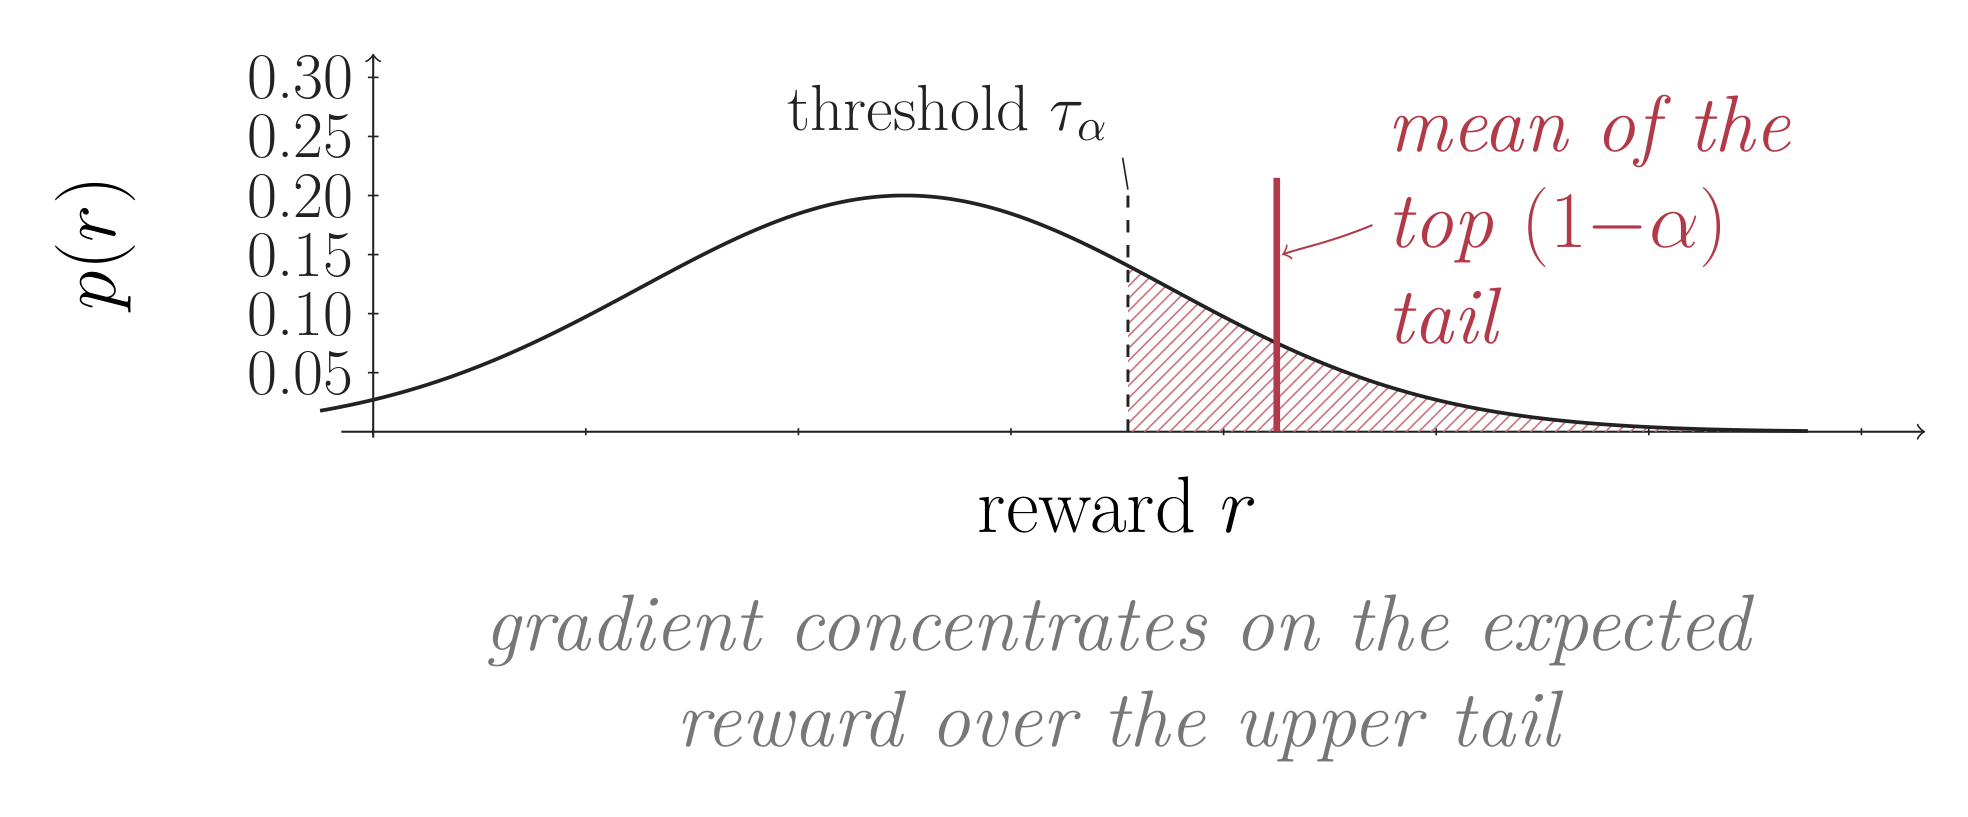
\includegraphics[width=\textwidth]{figures/diagram_cvar.png}\\
    \small (a) CVaR upper-tail reweighting
  \end{minipage}\hfill
  \begin{minipage}[t]{0.32\textwidth}\centering
    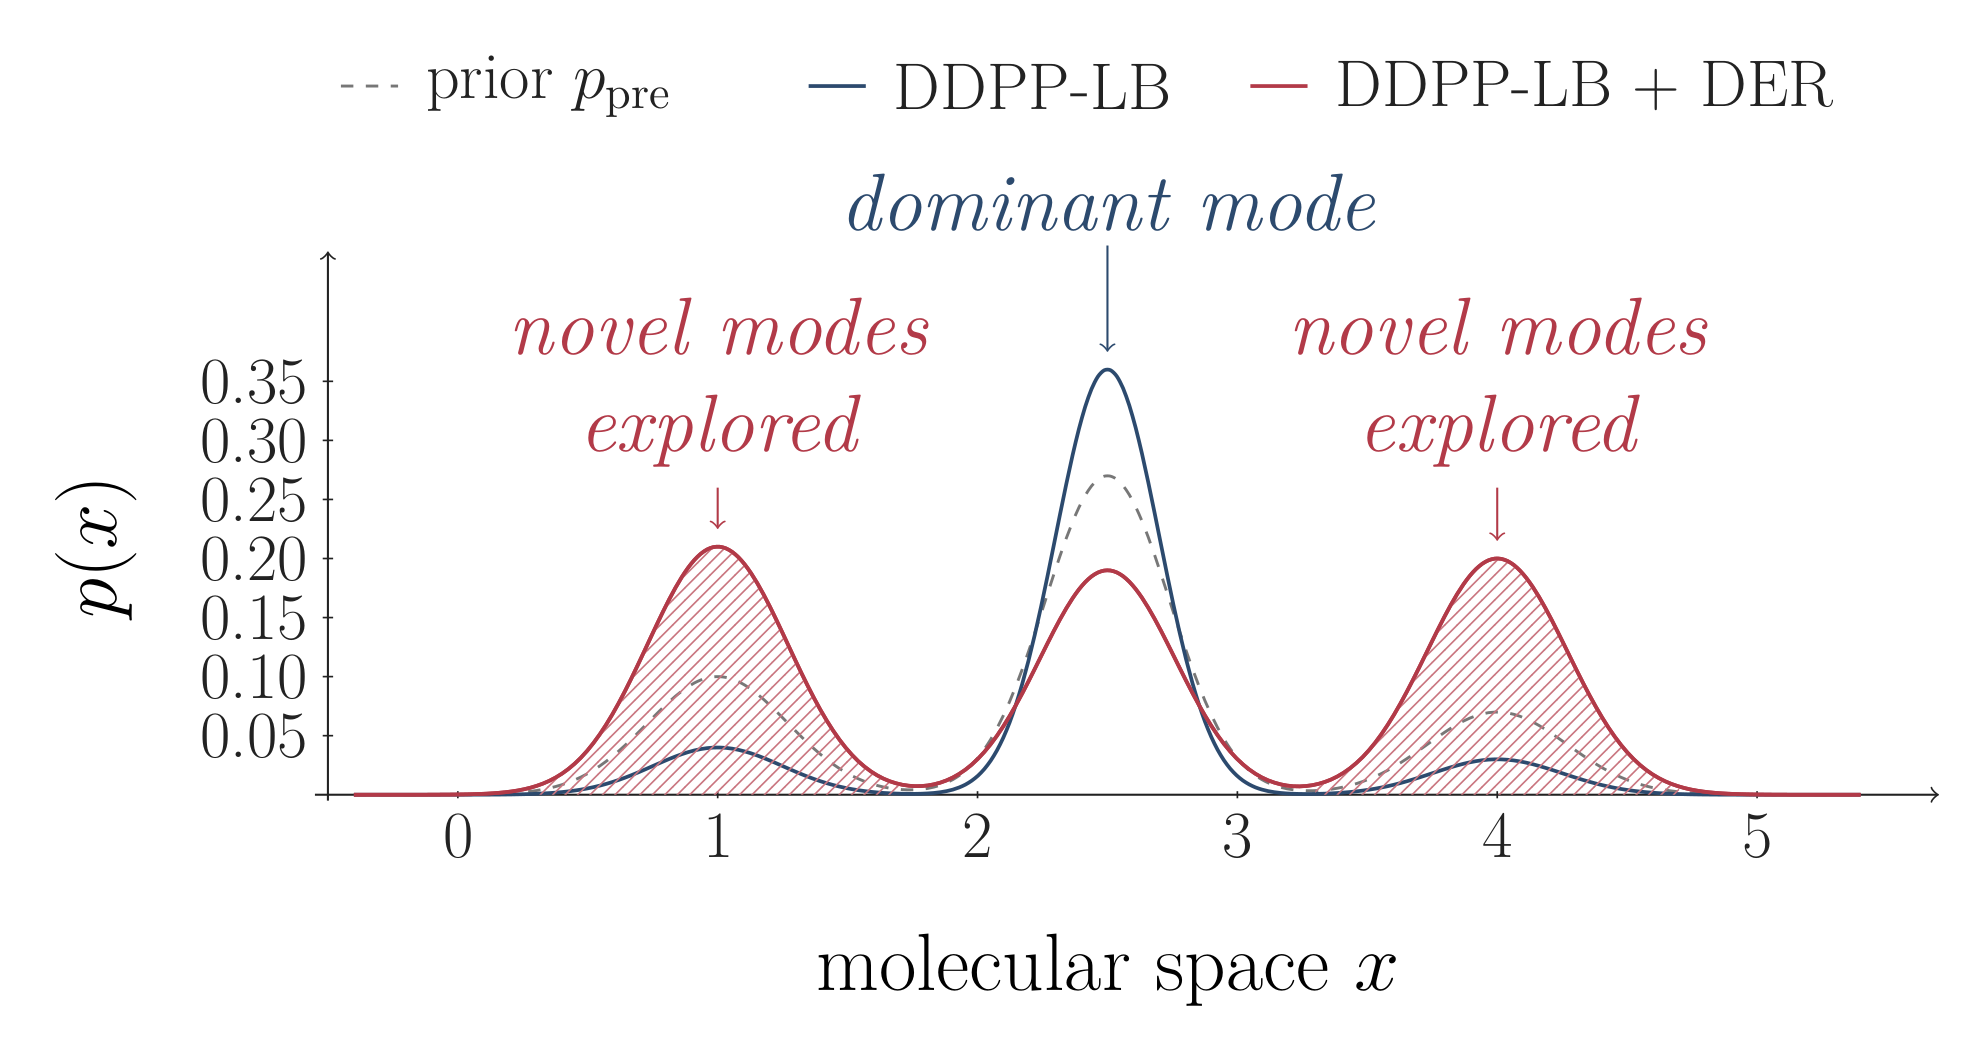
\includegraphics[width=\textwidth]{figures/diagram_debiasing.png}\\
    \small (b) Model debiasing (Density entropy regularization)
  \end{minipage}\hfill
  \begin{minipage}[t]{0.32\textwidth}\centering
    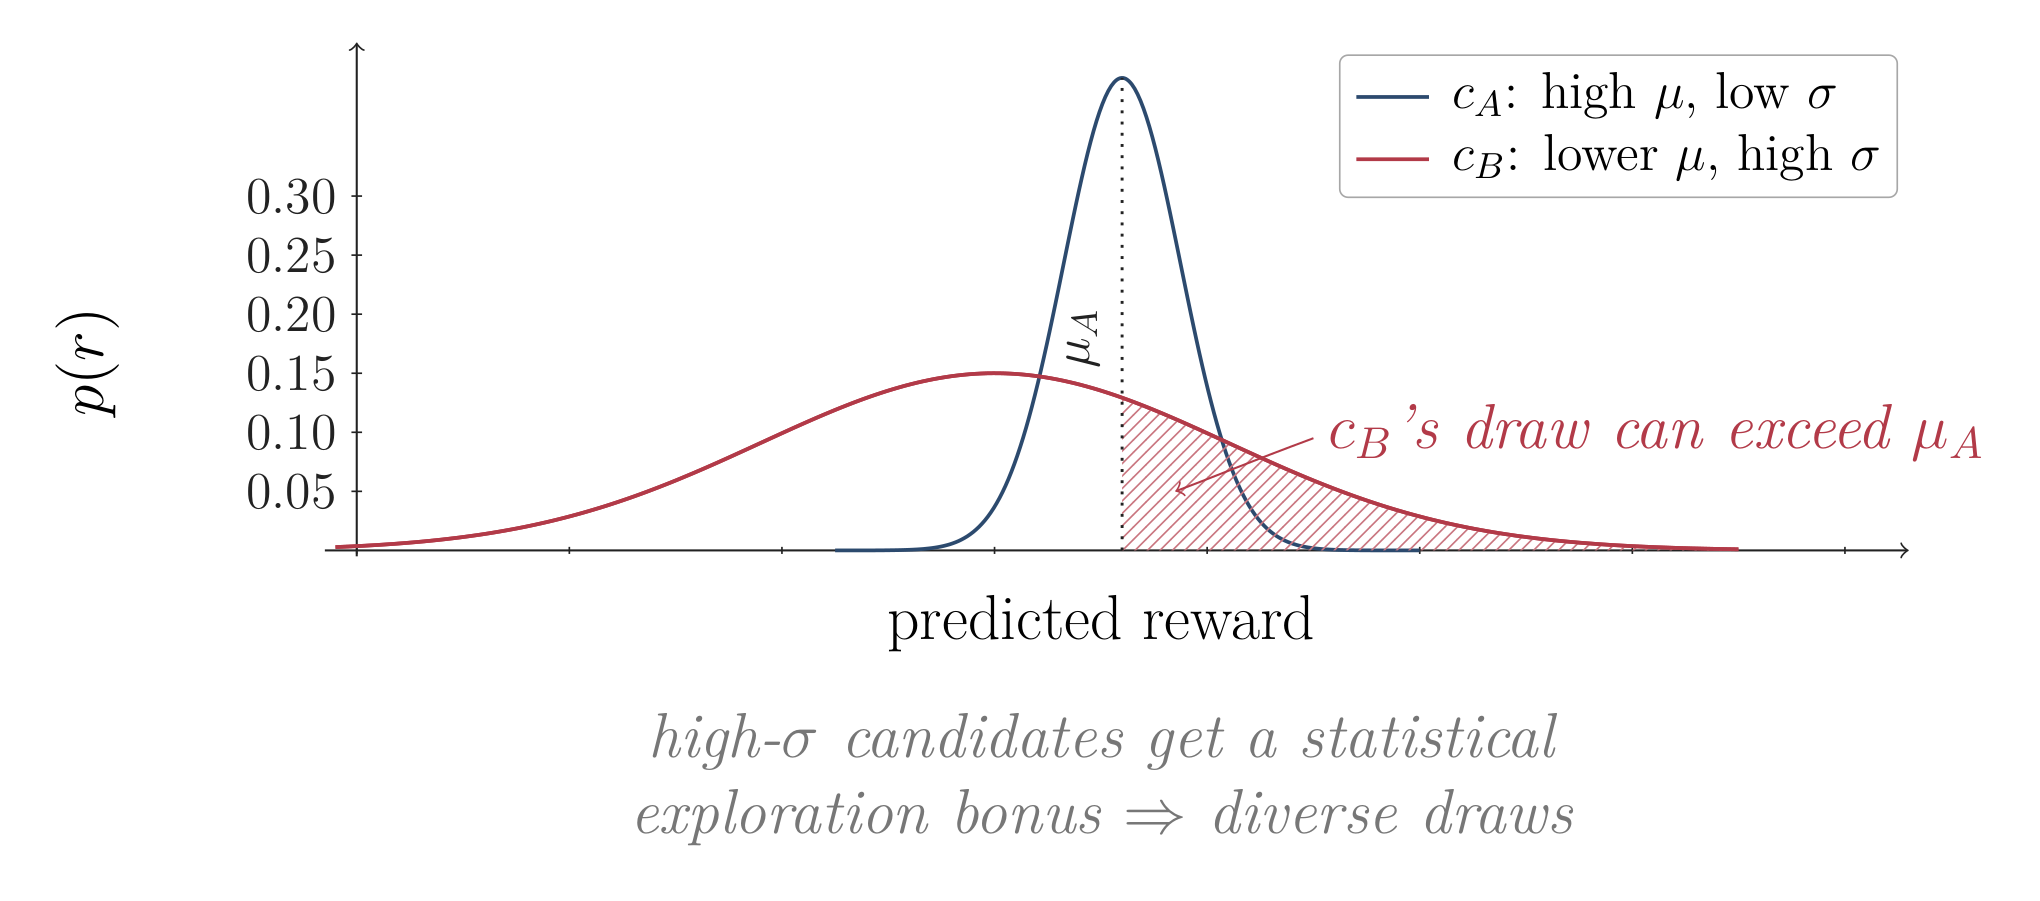
\includegraphics[width=\textwidth]{figures/diagram_thompson.png}\\
    \small (c) Thompson sampling
  \end{minipage}
  \caption{The three exploration knobs. \textbf{(a) CVaR$_{1-\tau}$} is the expected reward conditional on being above the $\tau$-quantile (Eq.~\ref{eq:cvar}); maximizing it concentrates gradient on the rare high-reward tail. \textbf{(b) Model debiasing} subtracts $\gamma \log p_{\theta_t}(x)$ from the shaped log-reward (Eq.~\ref{eq:debias}), penalizing mass on densely-occupied modes and redirecting exploration toward less-frequented regions. \textbf{(c) Thompson sampling} draws sampled surrogate rewards $\hat r_i = \mu_i + \varepsilon_i \sigma_i$ from each candidate's ensemble posterior; high-$\sigma$ candidates have fat tails and so occasionally beat the deterministic max-mean pick.}
  \label{fig:test_time_feedback}
  \label{fig:explore_knobs}
\end{figure}


\subsection{Experimental Setup}\label{sec:exp-setup}

We run controlled experiments to isolate the effect of each engineering choice on oracle (reward) sample efficiency. We study 9 total tasks split across two domains: (1) small molecule optimization for binding affinity to six different protein targets (2VT4, 5SDV, 6CM4, 7BKC, 7C7M, and 7YLL) and (2) protein fitness optimization across three different families (GB1, binding; CreiLOV, fluoresence; and TrpB, enzyme activity). 

For the small molecule task, our generative backbone is GenMol \citep{leeGenMolDrugDiscovery2025}, a discrete diffusion model over small-molecule SAFE strings \citep{noutahiGottaBeSAFE2023} and binding-affinity is evaluated using FlashAffinity (FA) \citep{jiangFlashAffinityBridgingAccuracySpeed} as an oracle. FA is fast and relatively inexpensive. On its own this raises the concern that improvements transfer trivially because the oracle is too easy, so wherever feasible we re-run the same experiment under Boltz-2 \citep{passaro2025boltz2}, a structure-prediction-based oracle that is orders of magnitude more expensive and therefore a more demanding test of generalization. For each protein task, our generative backbone is an MDLM discrete diffusion model \citep{sahooSimpleEffectiveMasked2024} trained over a protein family, and each oracle is a a computational surrogate trained over large amounts of real-world fitness data, as used in \cite{yangSteeringGenerativeModels2025}.

Each controlled experiment is run for five random seeds (\{0, 1, 2, 3, 42\}) on a single NVIDIA A100 80GB at a fixed wall budget of 10k oracle evaluations. Alongside the single best oracle score so far (top-1), we also log the running mean of the top-$k$ samples (top-$k$ mean) and the top-$k\%$ samples (top-$k\%$ mean), to capture not just the single best discovery but how the upper tail of the score distribution evolves. All three are reported both against cumulative oracle calls and against GPU hours. The two axes carry complementary information: per-oracle-call comparisons isolate sample efficiency independent of oracle cost, while per-GPU-hour comparisons fold in the realistic cost of running the oracle. Wall time for a single run decomposes as
\begin{equation}
t_{\text{wall}} \;=\; N \cdot c_{\text{oracle}} + C_{\text{method}},
\label{eq:wall-decomp}
\end{equation}
where $N$ is the number of oracle calls, $c_{\text{oracle}}$ is the per-call oracle cost, and $C_{\text{method}}$ collects all method-side compute (generation, fine-tuning steps, surrogate updates). Reporting against both axes reveals whether one technique dominates another regardless of oracle cost, or only past a threshold $c_{\text{oracle}}^\star$ at which the two curves cross.

Alongside the oracle score we monitor a sliding-window panel of secondary metrics (window size 300, stride 200) to watch for reward hacking: SMILES validity rate, pairwise Tanimoto diversity \citep{bajusz2015tanimoto} (computed as $1$ minus the mean Morgan-fingerprint Tanimoto similarity within the window), and per-molecule quality scores QED \citep{bickerton2012qed} and SA \citep{ertl2009sa}. A method that increases FA while collapsing diversity or degrading QED/SA is treated as reward-hacking the oracle rather than as a genuine improvement. Per-cell secondary-metric traces are reported in Appendix~\ref{app:traces}.

Final comparisons are run in two regimes, as illustrated in Fig.~\ref{fig:overview}. For small molecules we use GenMol \citep{leeGenMolDrugDiscovery2025}, a masked discrete diffusion model that decodes molecular SAFE sequences \citep{noutahiGottaBeSAFE2023} by parallel denoising of partially masked token sequences. At each diffusion time $t \in (0, 1]$ a fraction of tokens are masked, and the model learns the denoising posterior $p_{\text{pre}}(x_0 \mid x_t)$ that we treat as the frozen anchor throughout. The oracle is FlashAffinity (FA) \citep{jiangFlashAffinityBridgingAccuracySpeed}, a fast neural binding-affinity model that scores a (ligand, pocket) pair in tens of milliseconds. We extend the comparison across six protein binding pockets: 2VT4, 5SDV, 6CM4, 7BKC, 7C7M, and 7YLL. For proteins, \todo{Ariel: backbone model, target set, and oracle.}

\begin{figure}[H]
  \centering
  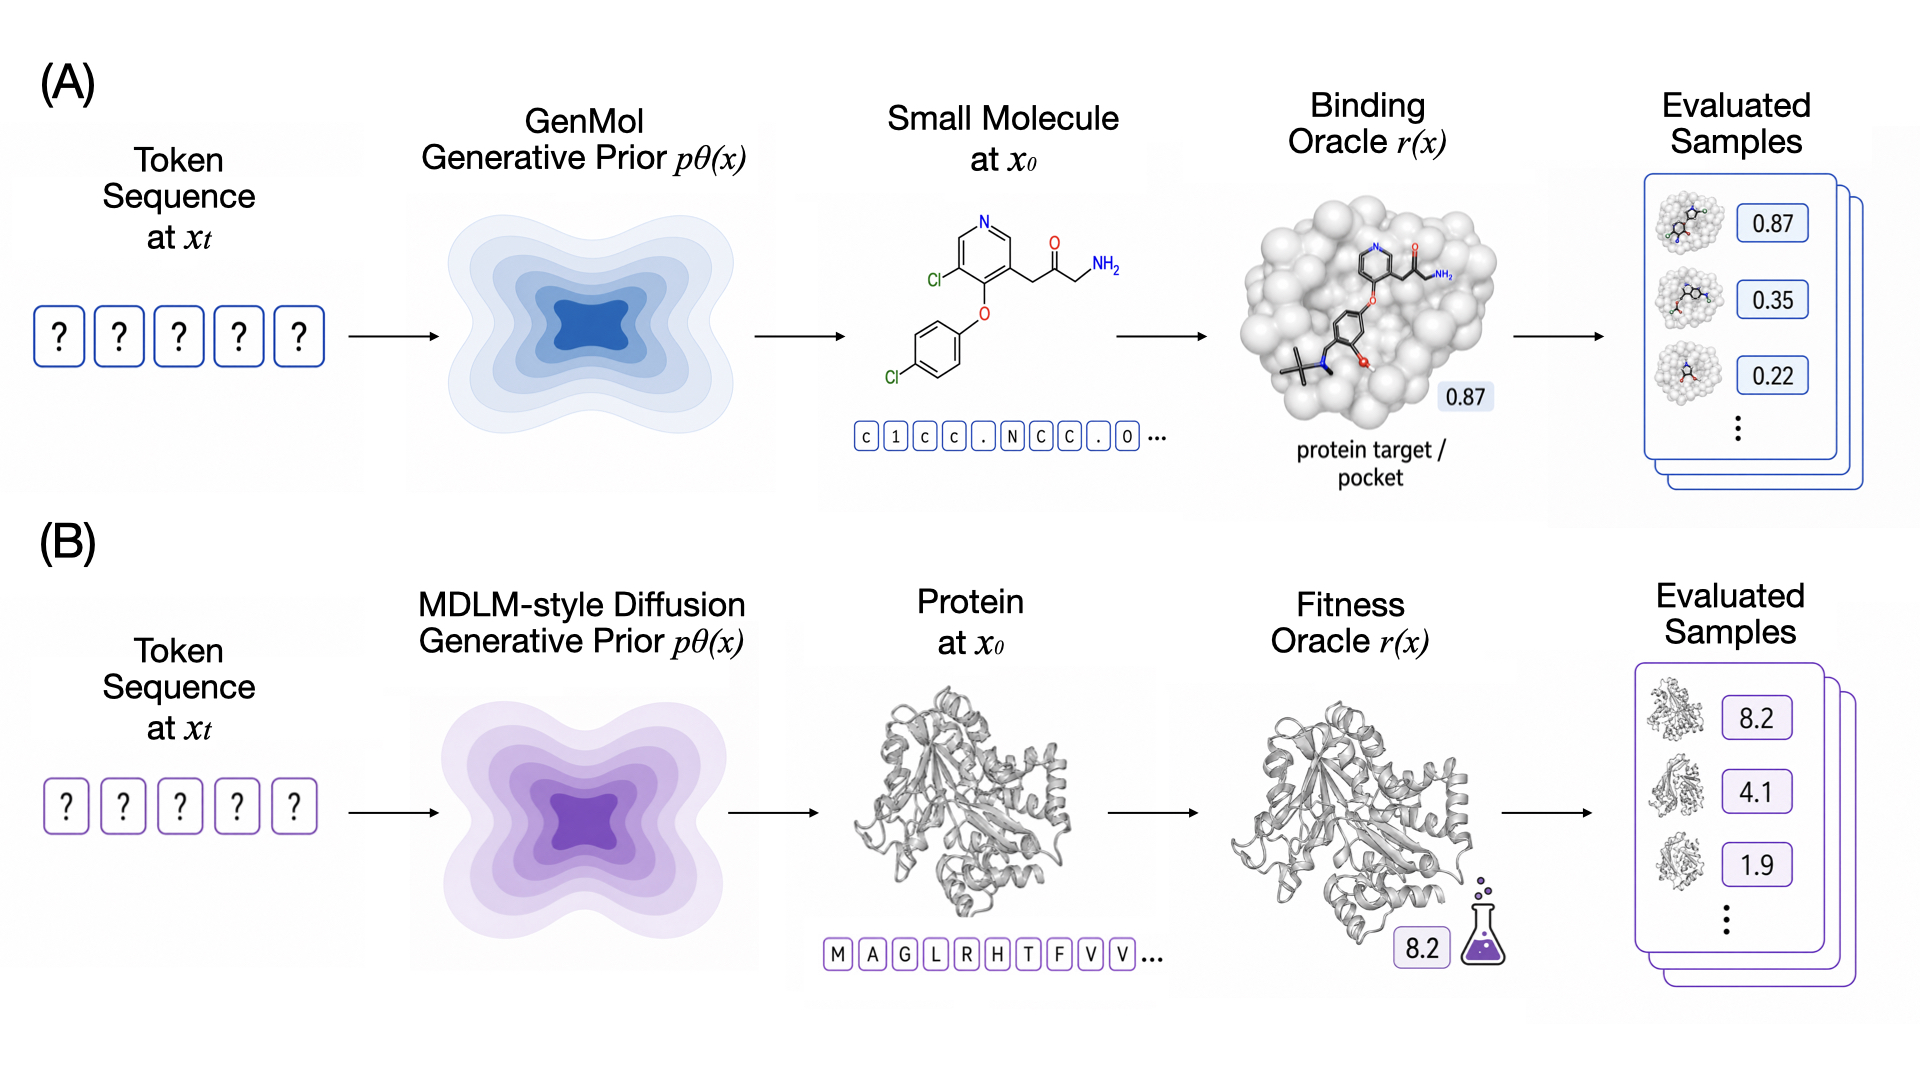
\includegraphics[width=\textwidth]{figures_source/Applications002.jpeg}
  \caption{A useful paradigm for molecular optimization involves steering generative priors with expensive reward evaluations at test time. In this study, we explore two different tasks, \textbf{(A)} small molecules for binding to protein targets and \textbf{(B)} proteins for various fitness metrics.}
  \label{fig:overview}
\end{figure}

Table~\ref{tab:methods} summarizes every experimental configuration we evaluate, grouped by family. Per-knob individual controlled experiments are reported in Appendix~\ref{app:knobs}.
T
\begin{table}[ht]
\centering
\small
\begin{tabular}{@{}p{4.4cm}p{9.3cm}@{}}
\toprule
\textbf{Knob} & \textbf{Description} \\
\midrule
$+$ CVaR             & Replace $r$ with $(r - Q_\tau)_+/(1-\tau)$, $\tau{=}0.8$ \\
$+$ Annealed CVaR    & CVaR with $\tau$ scheduled $0 \rightarrow 0.99$ over wall time \\
$+$ Model debiasing  & Add $-\gamma \log p_{\theta_t}(x)$ to log-reward, $\gamma{=}1$ \\
$+$ Thompson         & $J{=}10$ MLP ensemble; oracle top-$K$ by $\hat r_i \sim \mathcal{N}(\mu_i, \sigma_i^2)$ \\
$+$ Replay buffer    & Fixed-capacity FIFO with priority eviction; stratified sampling \\
$+$ Invalid penalty  & Assign $r {=} r_{\text{inv}}$ to SMILES that fail RDKit parsing \\
\bottomrule
\end{tabular}
\caption{\textbf{Composable knobs evaluated in this paper.} Each knob layers on top of online DDPP-LB and is ablated independently in Section~\ref{sec:results}, then combined into the final algorithm of Sec.~\ref{sec:results-method}. Search-only and offline-fine-tuning baselines used for context (unconditional, beam, MCTS, DFKC, offline DDPP-LB) are described inline in Sec.~\ref{sec:related} and the corresponding Appendix figures.}
\label{tab:methods}
\end{table}

\fi



% % Previous float placement retained for recovery: \begin{figure}[t!]
% \begin{figure}[H]
%   \centering
%   
%   % \vspace{-0.10in} % disabled to restore figure spacing
%   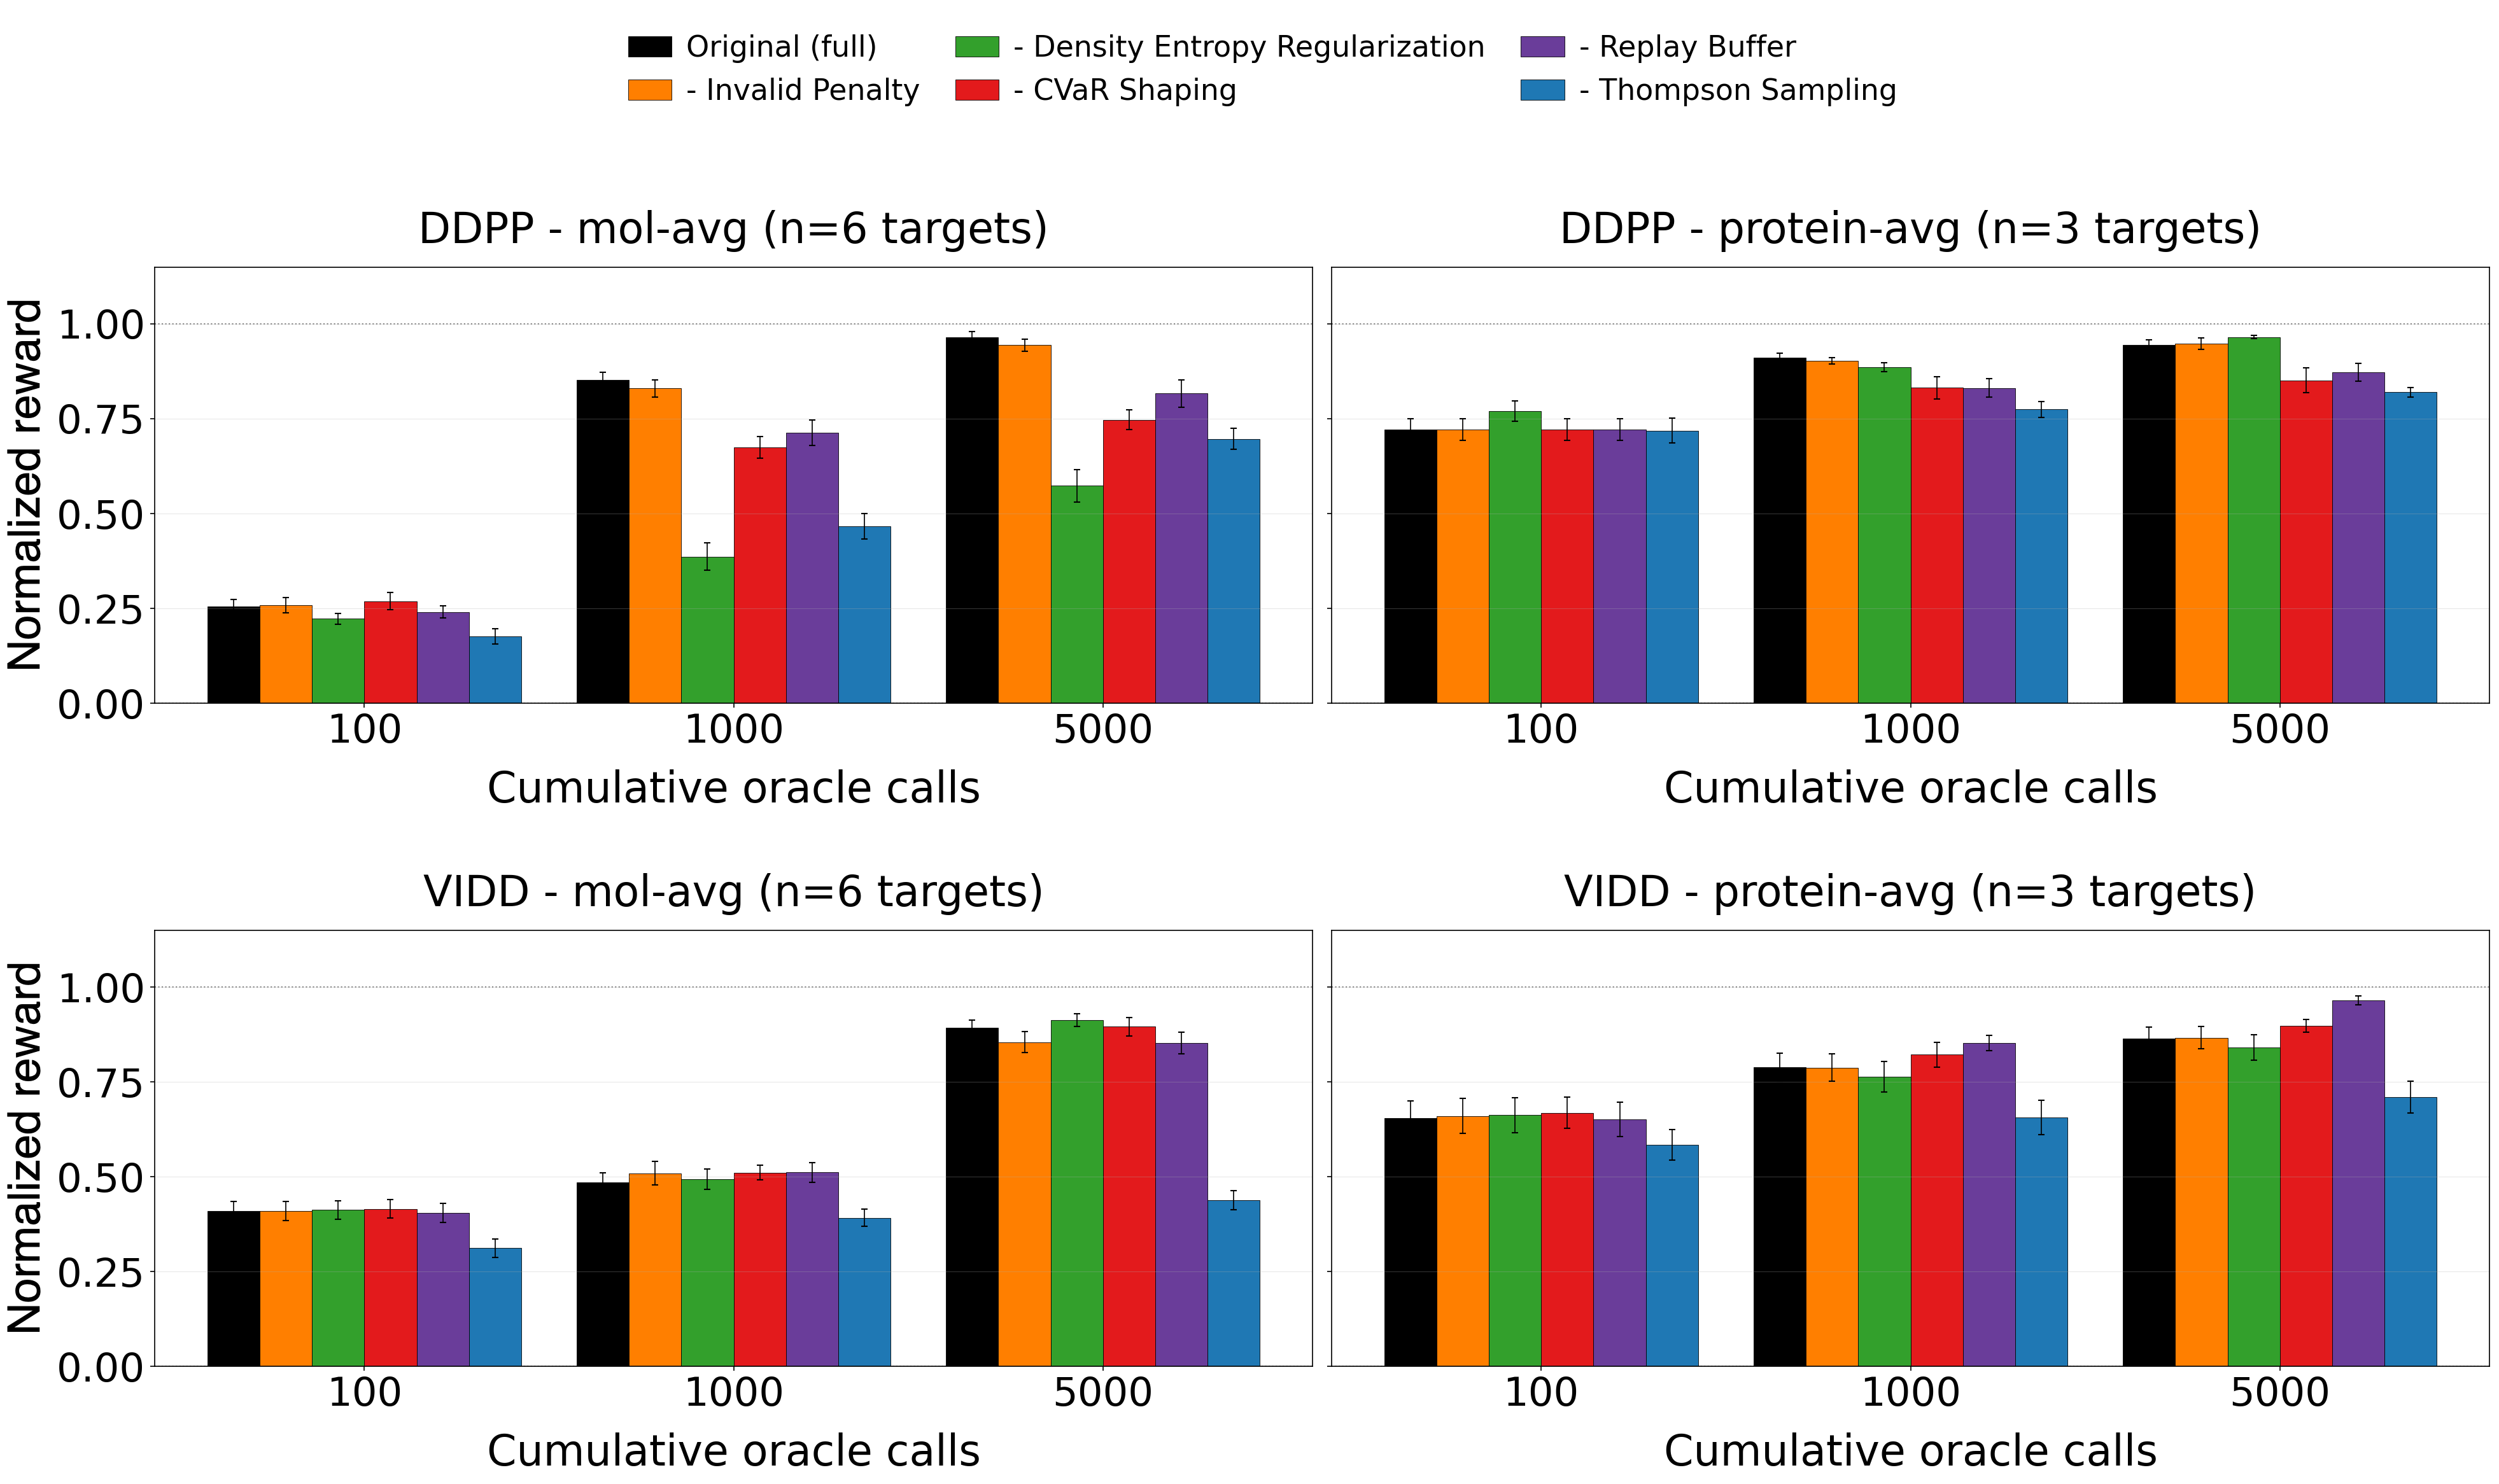
\includegraphics[width=0.90\textwidth]{figures/ablations/result1_combined_vs_baseline_1.png}
%   % \vspace{-0.2in} % disabled to restore figure spacing
%    \caption{\textbf{Leave-one-out ablations reveal complementary roles most clearly on small-molecule tasks.} Normalised reward at 100/1k/5k calls for DDPP-LB (top) and VIDD (bottom), averaged over molecule targets (left) and protein families (right). Small-molecule effects are strongest for Density Entropy Regularization; protein effects are weaker, with Thompson sampling clearest. Error bars: $\pm1$ SEM over target--seed runs; Appendix~\ref{app:knobs} gives tables.}
% % Previous full caption retained for recovery.
% % \caption{\textbf{Leave-one-out ablations reveal complementary roles most clearly on small-molecule tasks.} Each panel removes one component from the full online loop and reports normalised maximum reward after 100, 1k, and 5k oracle calls, for DDPP-LB (top) and VIDD (bottom), averaged over small-molecule targets (left) and protein families (right). At later budgets, small-molecule ablations diverge most strongly, with Density Entropy Regularization producing the largest drop; protein-fitness ablations are weaker, with Thompson sampling giving the clearest consistent gain. Error bars show $\pm 1$ SEM over target-seed runs. Reward is normalised per target before averaging; see Eq.~\ref{eq:lift}. Tabular values are reported in Appendix~\ref{app:knobs}.}
% \label{fig:barplot_ablation}
%     % \vspace{-0.1in} % disabled to restore figure spacing
% \end{figure}

% \begin{samepage} % disabled; Results now begins on a fresh page
\newpage
\section{Results}\label{sec:results}

%Our main finding is that each of the design choices described in Section~\ref{sec:design-space} contribute meaningfully to performance for molecular optimization, as shown in Fig.~\ref{fig:barplot_ablation}. The results are less conclusive for protein optimization (with the exception of using Thompson Sampling), possibly because high-reward proteins are already well represented by protein diffusion generator's prior distribution.  Sec.~\ref{sec:results-method} provides a breakdown of our primary controlled study.  Sec.~\ref{sec:analysis} provides further analysis on how different components affect the distribution of the fine-tuned generator.

Our main finding is that the online-loop components are complementary, although not equally so across domains (Fig.~\ref{fig:barplot_ablation}). On small molecules, acquisition, CVaR reward shaping, and Density Entropy Regularization produce the clearest reward gains, while replay and validity penalties stabilize the exploratory loop. On protein-fitness tasks, ablation effects are weaker and Thompson sampling gives the clearest consistent gain, suggesting that the family-specific priors already cover high-fitness regions more closely. Sec.~\ref{sec:results-method} breaks down the controlled ablations, and Sec.~\ref{sec:analysis} analyzes how these components shift the fine-tuned generator's distribution.
% \end{samepage} % disabled

\begin{figure}[H]
  \centering
  
  % \vspace{-0.10in} % disabled to restore figure spacing
  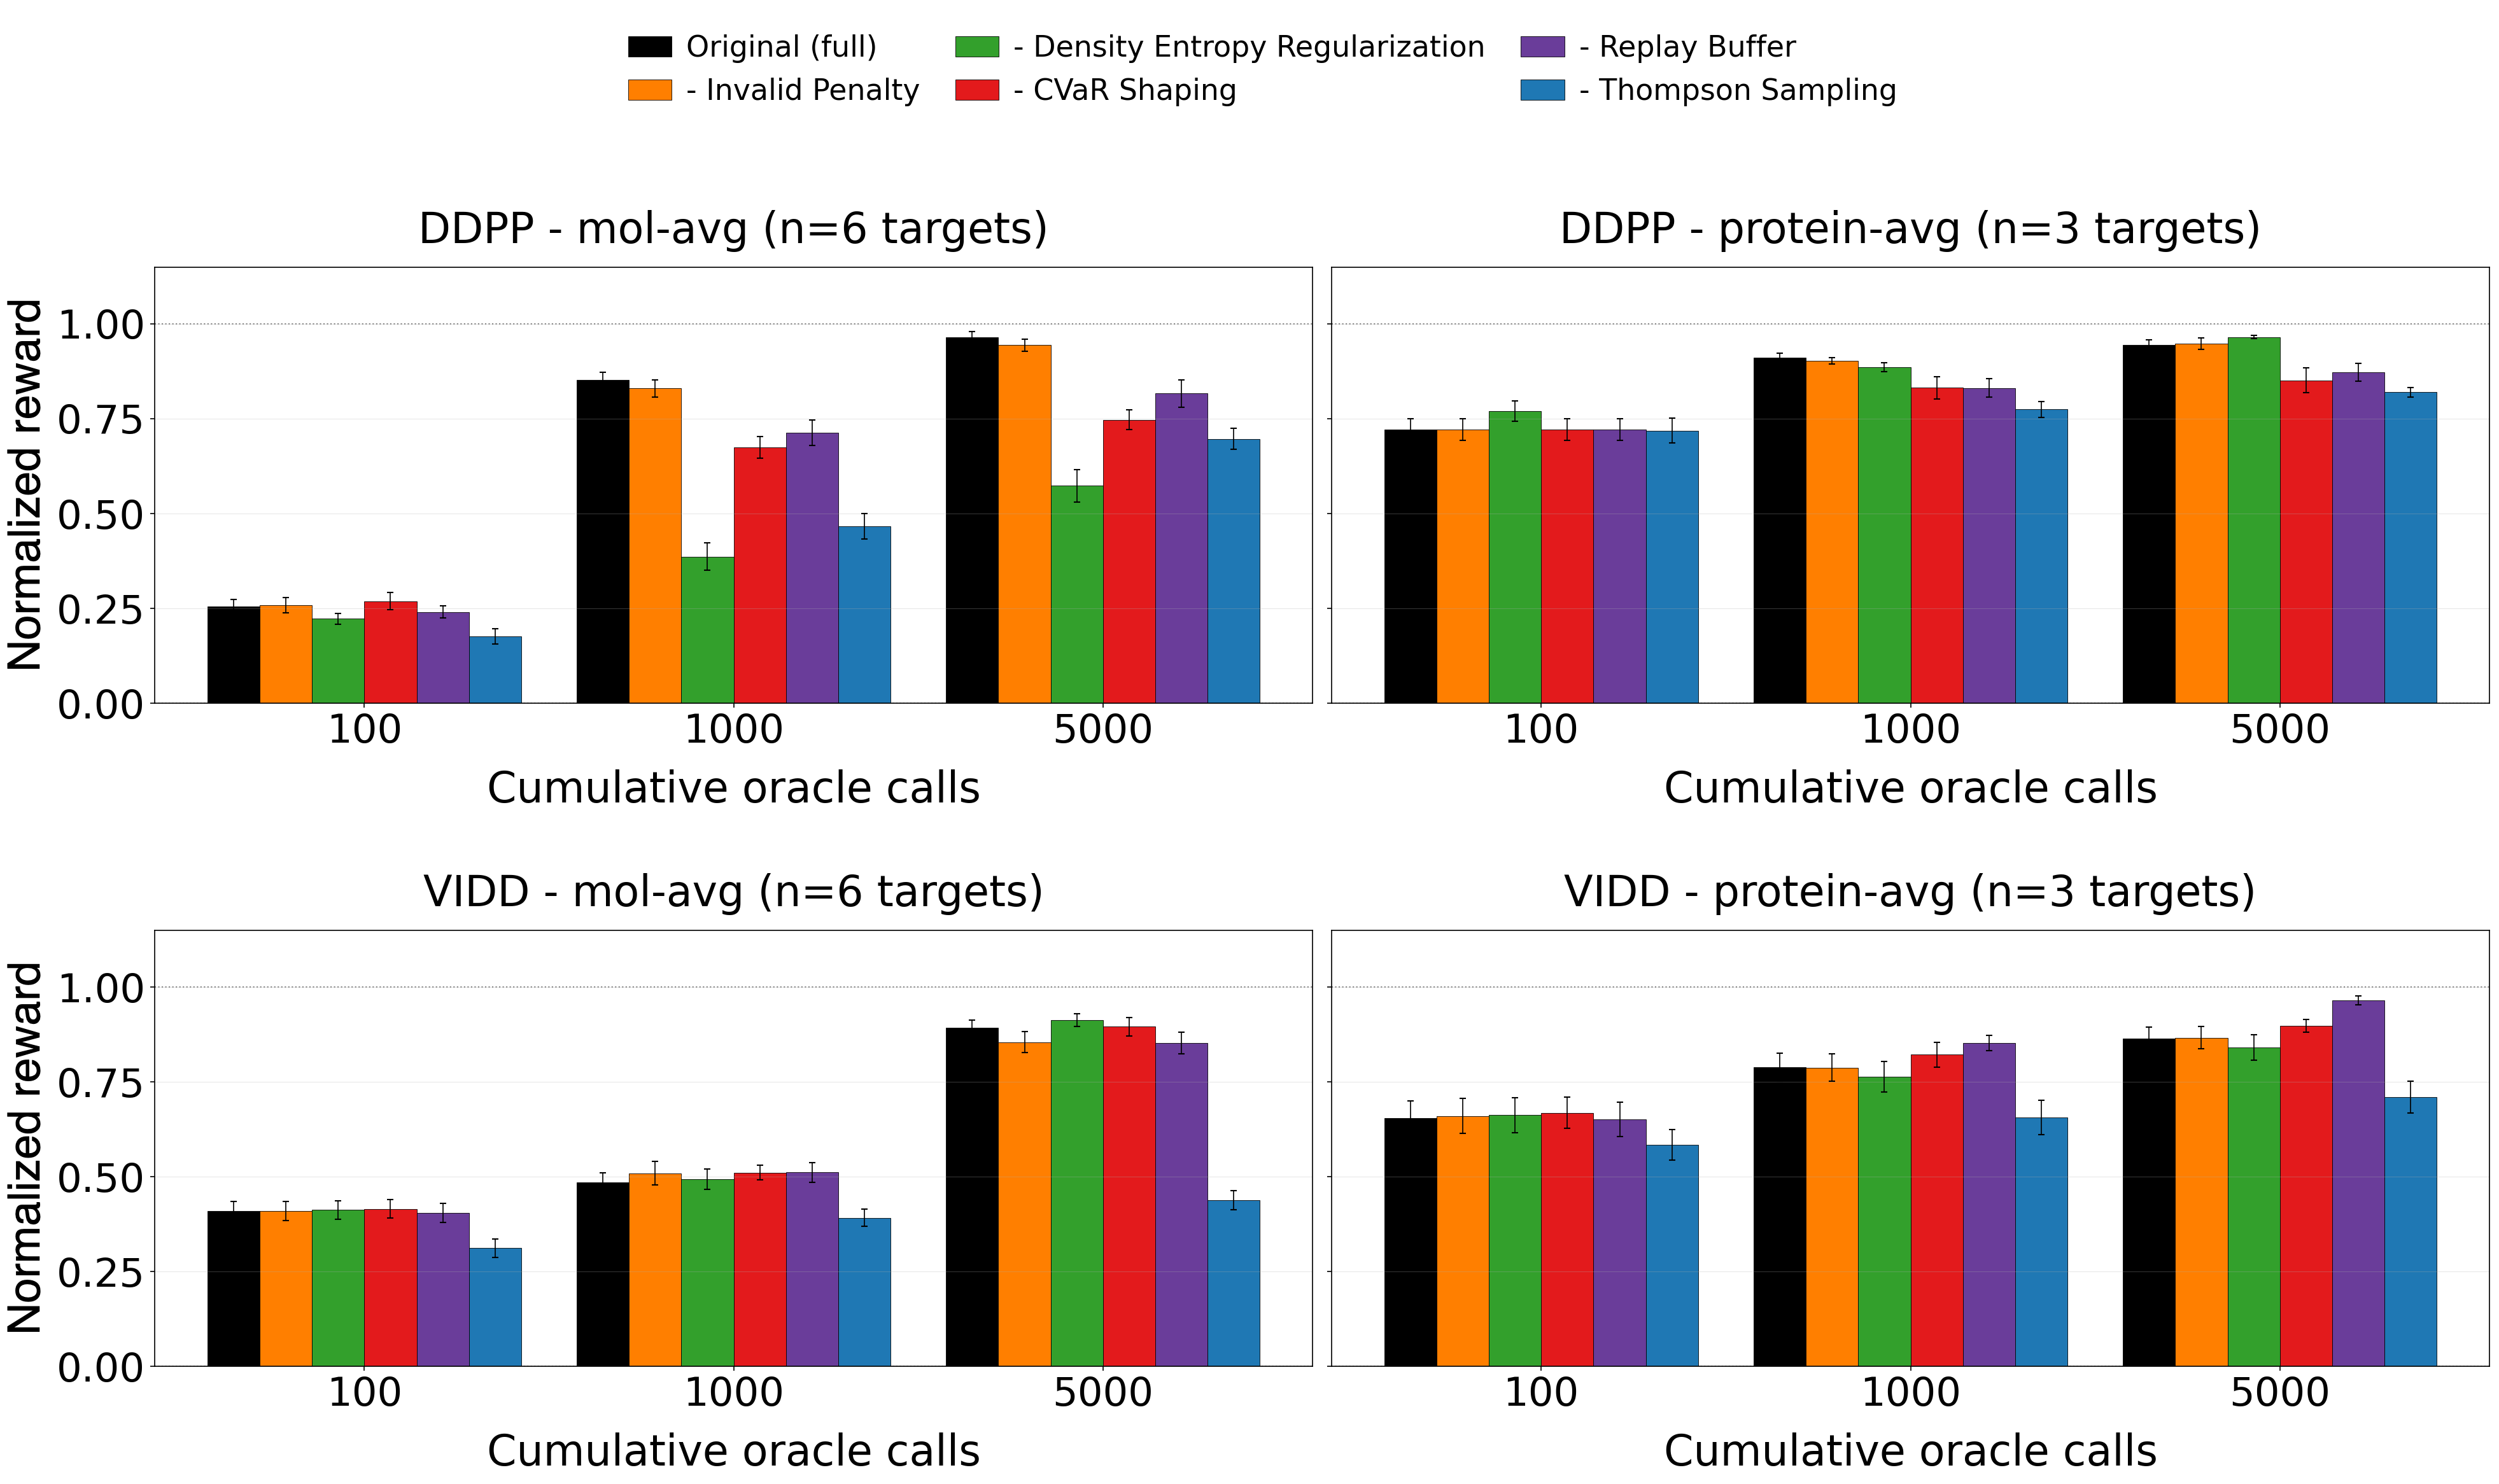
\includegraphics[width=0.90\textwidth]{figures/ablations/result1_combined_vs_baseline_1.png}
  % \vspace{-0.2in} % disabled to restore figure spacing
   \caption{\textbf{Leave-one-out ablations reveal complementary roles most clearly on small-molecule tasks.} Normalised reward at 100/1k/5k calls for DDPP-LB (top) and VIDD (bottom), averaged over molecule targets (left) and protein families (right). Small-molecule effects are strongest for Density Entropy Regularization; protein effects are weaker, with Thompson sampling clearest. Error bars: $\pm1$ SEM over target--seed runs; Appendix~\ref{app:knobs} gives tables.}
% Previous full caption retained for recovery.
% \caption{\textbf{Leave-one-out ablations reveal complementary roles most clearly on small-molecule tasks.} Each panel removes one component from the full online loop and reports normalised maximum reward after 100, 1k, and 5k oracle calls, for DDPP-LB (top) and VIDD (bottom), averaged over small-molecule targets (left) and protein families (right). At later budgets, small-molecule ablations diverge most strongly, with Density Entropy Regularization producing the largest drop; protein-fitness ablations are weaker, with Thompson sampling giving the clearest consistent gain. Error bars show $\pm 1$ SEM over target-seed runs. Reward is normalised per target before averaging; see Eq.~\ref{eq:lift}. Tabular values are reported in Appendix~\ref{app:knobs}.}
\label{fig:barplot_ablation}
    % \vspace{-0.1in} % disabled to restore figure spacing
\end{figure}

% \newpage % disabled to avoid the half-empty Results page
\subsection{Individual harness design components complement each other}\label{sec:results-method}


\textbf{Steering Design Choices.}
Thompson sampling gives the clearest acquisition-side gain in the main leave-one-out ablations (Fig.~\ref{fig:barplot_ablation}). In the isolated Thompson ablation, its strongest effect appears in the top-10\% mean rather than in top-1 alone, consistent with its role in diversifying which candidates receive oracle calls and shifting the generated distribution toward higher-reward modes (Appendix Fig.~\ref{fig:thompson_ablation}).
In contrast, adding inference-time search to the online loop (best-of-$N$, beam, MCTS, DFKC, or SMC) does not improve over plain online fine-tuning at fixed wall budget (Appendix Fig.~\ref{fig:tweedie_active}). The reason is primarily compute allocation: search proposes $L \times M$ candidates per round instead of $M$, and the extra forward passes needed to score and prune them dominate the wall budget, leaving little time for fine-tuning gradient steps (Appendix Figs.~\ref{fig:search_overhead}, \ref{fig:tweedie_active_compute}, \ref{fig:compute_breakdown}). Under this budget, each gradient step extracts more reusable signal from an oracle call than one-shot search does.

%Thompson sampling provides consistent and substantial increases the maximum reward achieved (Fig. \ref{fig:barplot_ablation}); its effect additionally concentrates on top-1 rather than top-10\% mean, consistent with its role at the acquisition step rather than at gradient computation (Appendix Fig.~\ref{fig:thompson_ablation}). Interestingly, augmenting online adaptation with search (best-of-$N$, beam, MCTS, DFKC, and SMC) does not outperform plain online finetuning at fixed wall budget (Appendix Fig.~\ref{fig:tweedie_active}). The reason largely comes down to compute allocation: per-phase wall-time decomposition (Appendix Figs.~\ref{fig:search_overhead}, \ref{fig:tweedie_active_compute}, \ref{fig:compute_breakdown}) shows that search produces $L \times M$ candidates per epoch instead of $M$, and the extra forward passes through $p_{\theta_t}$ to score and prune them dominate the wall budget, leaving little time for fine-tuning gradient steps. Each gradient step extracts more usable signal per oracle call than a one-shot search evaluation, so plain online finetuning wins the budget tradeoff. %Retroactively rescaling per-call oracle cost by $100\times$ (a Boltz-2-class regime) does not flip the conclusion (Appendix Fig.~\ref{fig:oracle_rescale}).

%\textbf{Adaptation Design Choices.} 
%CVaR reward shaping and Density Entropy Regularization provide the clearest reward gains on small-molecule tasks (Fig.~\ref{fig:barplot_ablation}). Appendix Fig.~\ref{fig:cvar_ablation} compares CVaR-on vs.\ CVaR-off across online and offline DDPP, while Appendix Fig.~\ref{fig:debiasing_ablation} isolates Density Entropy Regularization by holding CVaR off. The two effects are not additive. A full $2\times2\times2$ factorial over Density Entropy Regularization, CVaR, and Thompson sampling (Appendix~\ref{app:factorial}) shows that each component's marginal value grows once the others are active, with Density Entropy Regularization acting as a gate: with it off, the remaining knobs move the score little, while with it on they move it substantially. This is the sense in which we call the components complementary --- each component's marginal value depends on which others are active, and that dependence is positive --- rather than either additive or redundant. They nonetheless target different failure modes: CVaR focuses updates on the reward tail, while Density Entropy Regularization pushes exploration away from modes already occupied by the current generator. Sec.~\ref{sec:analysis} analyzes these distributional effects directly.

\textbf{Component Interactions.} The complete $2 \times 2 \times 2$ factorial in Table~\ref{tab:factorial} demonstrates that DER, CVaR, and Thompson acquisition exhibit compounding synergy rather than simple additivity. We interpret this pattern as a gating interaction: DER acts as a gate because Thompson and CVaR operate relative to the current generator's support $p_{\theta_t}$. Without DER, $p_{\theta_t}$ remains confined to high-density prior modes where surrogate disagreement is low and upper-quantile updates simply sharpen local modes. Conversely, DER alone disperses proposals broadly into low-likelihood regions without selective filtering. Once DER pushes $p_{\theta_t}$ into unfamiliar off-prior space, Thompson sampling is required to translate the resulting surrogate uncertainty into non-redundant oracle evaluations, while CVaR is required to suppress off-prior exploratory noise and concentrate gradient steps on the newly discovered upper tail.

\begin{table}[H]
\centering
\small
\begin{tabular}{@{}cccr@{}}
\toprule
DER & CVaR & Thompson & Score \\
\midrule
on  & on  & on  & $+1.13$ \\
on  & off & on  & $+0.54$ \\
on  & on  & off & $-0.20$ \\
on  & off & off & $-0.43$ \\
off & on  & on  & $-0.54$ \\
off & off & on  & $-0.80$ \\
off & on  & off & $-0.86$ \\
off & off & off & $-1.06$ \\
\bottomrule
\end{tabular}

\vspace{6pt}
\caption{\textbf{All eight combinations of DER, CVaR, and Thompson (DDPP-LB).} Mean best oracle score at $1{,}000$ oracle calls, averaged over $30$ target--seed pairs. Turned on alone from the all-off cell ($-1.06$), DER is worth $+0.63$, Thompson $+0.26$, and CVaR $+0.20$; their individual gains sum to $+1.09$, falling well short of the $+2.19$ joint improvement.}
\label{tab:factorial}
\end{table}
\vspace{-22pt}

%CVaR and Density Entropy Regularization both consistently improve performance for molecular optimization (Fig. \ref{fig:barplot_ablation}).   Appendix Fig.~\ref{fig:cvar_ablation} futher compares CVaR-on vs.\ CVaR-off across online and offline DDPP; Appendix Fig.~\ref{fig:debiasing_ablation} compares Density Entropy Regularization-on vs.\ -off with CVaR held off, isolating the debiasing effect. The two knobs appear close to additive on maximum reward, consistent with the independent-failure-mode framing in Sec.~\ref{sec:design-space}. Sec.~\ref{sec:analysis} provides a more in depth analysis of the effects of CVaR shaping and density entropy regularization on the fine-tuned generator's distribution.
\textbf{Objective-Mismatch Corrections.} 
Replay and invalid-output penalties have smaller and less uniform effects on top-1 reward (Fig.~\ref{fig:barplot_ablation}), but they stabilize failure modes induced by exploration. The replay buffer has its clearest effect on top-10\% mean (Appendix Fig.~\ref{fig:buffer_ablation}), consistent with aligning the gradient with the time-averaged distribution of evaluated data rather than only the current on-policy batch. The invalid-output penalty prevents a sharper failure: without a validity penalty ($r_{\text{inv}}{=}0$), validity collapses within the first hour as the model concentrates mass on out-of-distribution but high-surrogate-reward strings~\citep{wangFineTuningDiscreteDiffusion2024, ueharaELEGANT2024}. This collapse is driven primarily by the likelihood penalty in Density Entropy Regularization (Appendix~\ref{app:knobs}), so validity control is best viewed as a guardrail for aggressive exploration rather than as a standalone reward booster.
%The replay buffer and invalid output penalty play a less consistent role (Fig. \ref{fig:barplot_ablation}), but mode collapse on several examples. Interestingly, the buffer's effect on top-10\% mean is the largest of any single design component (Appendix Fig.~\ref{fig:buffer_ablation}), consistent with its role aligning the gradient with the time-averaged distribution of evaluated data rather than the on-policy batch. Without a validity penalty ($r_{\text{inv}}{=}0$), validity collapses within the first hour as the model concentrates mass on out-of-distribution but high-surrogate-reward molecules \citep{wangFineTuningDiscreteDiffusion2024, ueharaELEGANT2024}. The collapse is driven primarily by Density Entropy Regularization's likelihood penalty (Appendix~\ref{app:knobs}).
\begin{figure}[H]
  \centering
  % \vspace{-0.10in} % disabled to restore figure spacing
  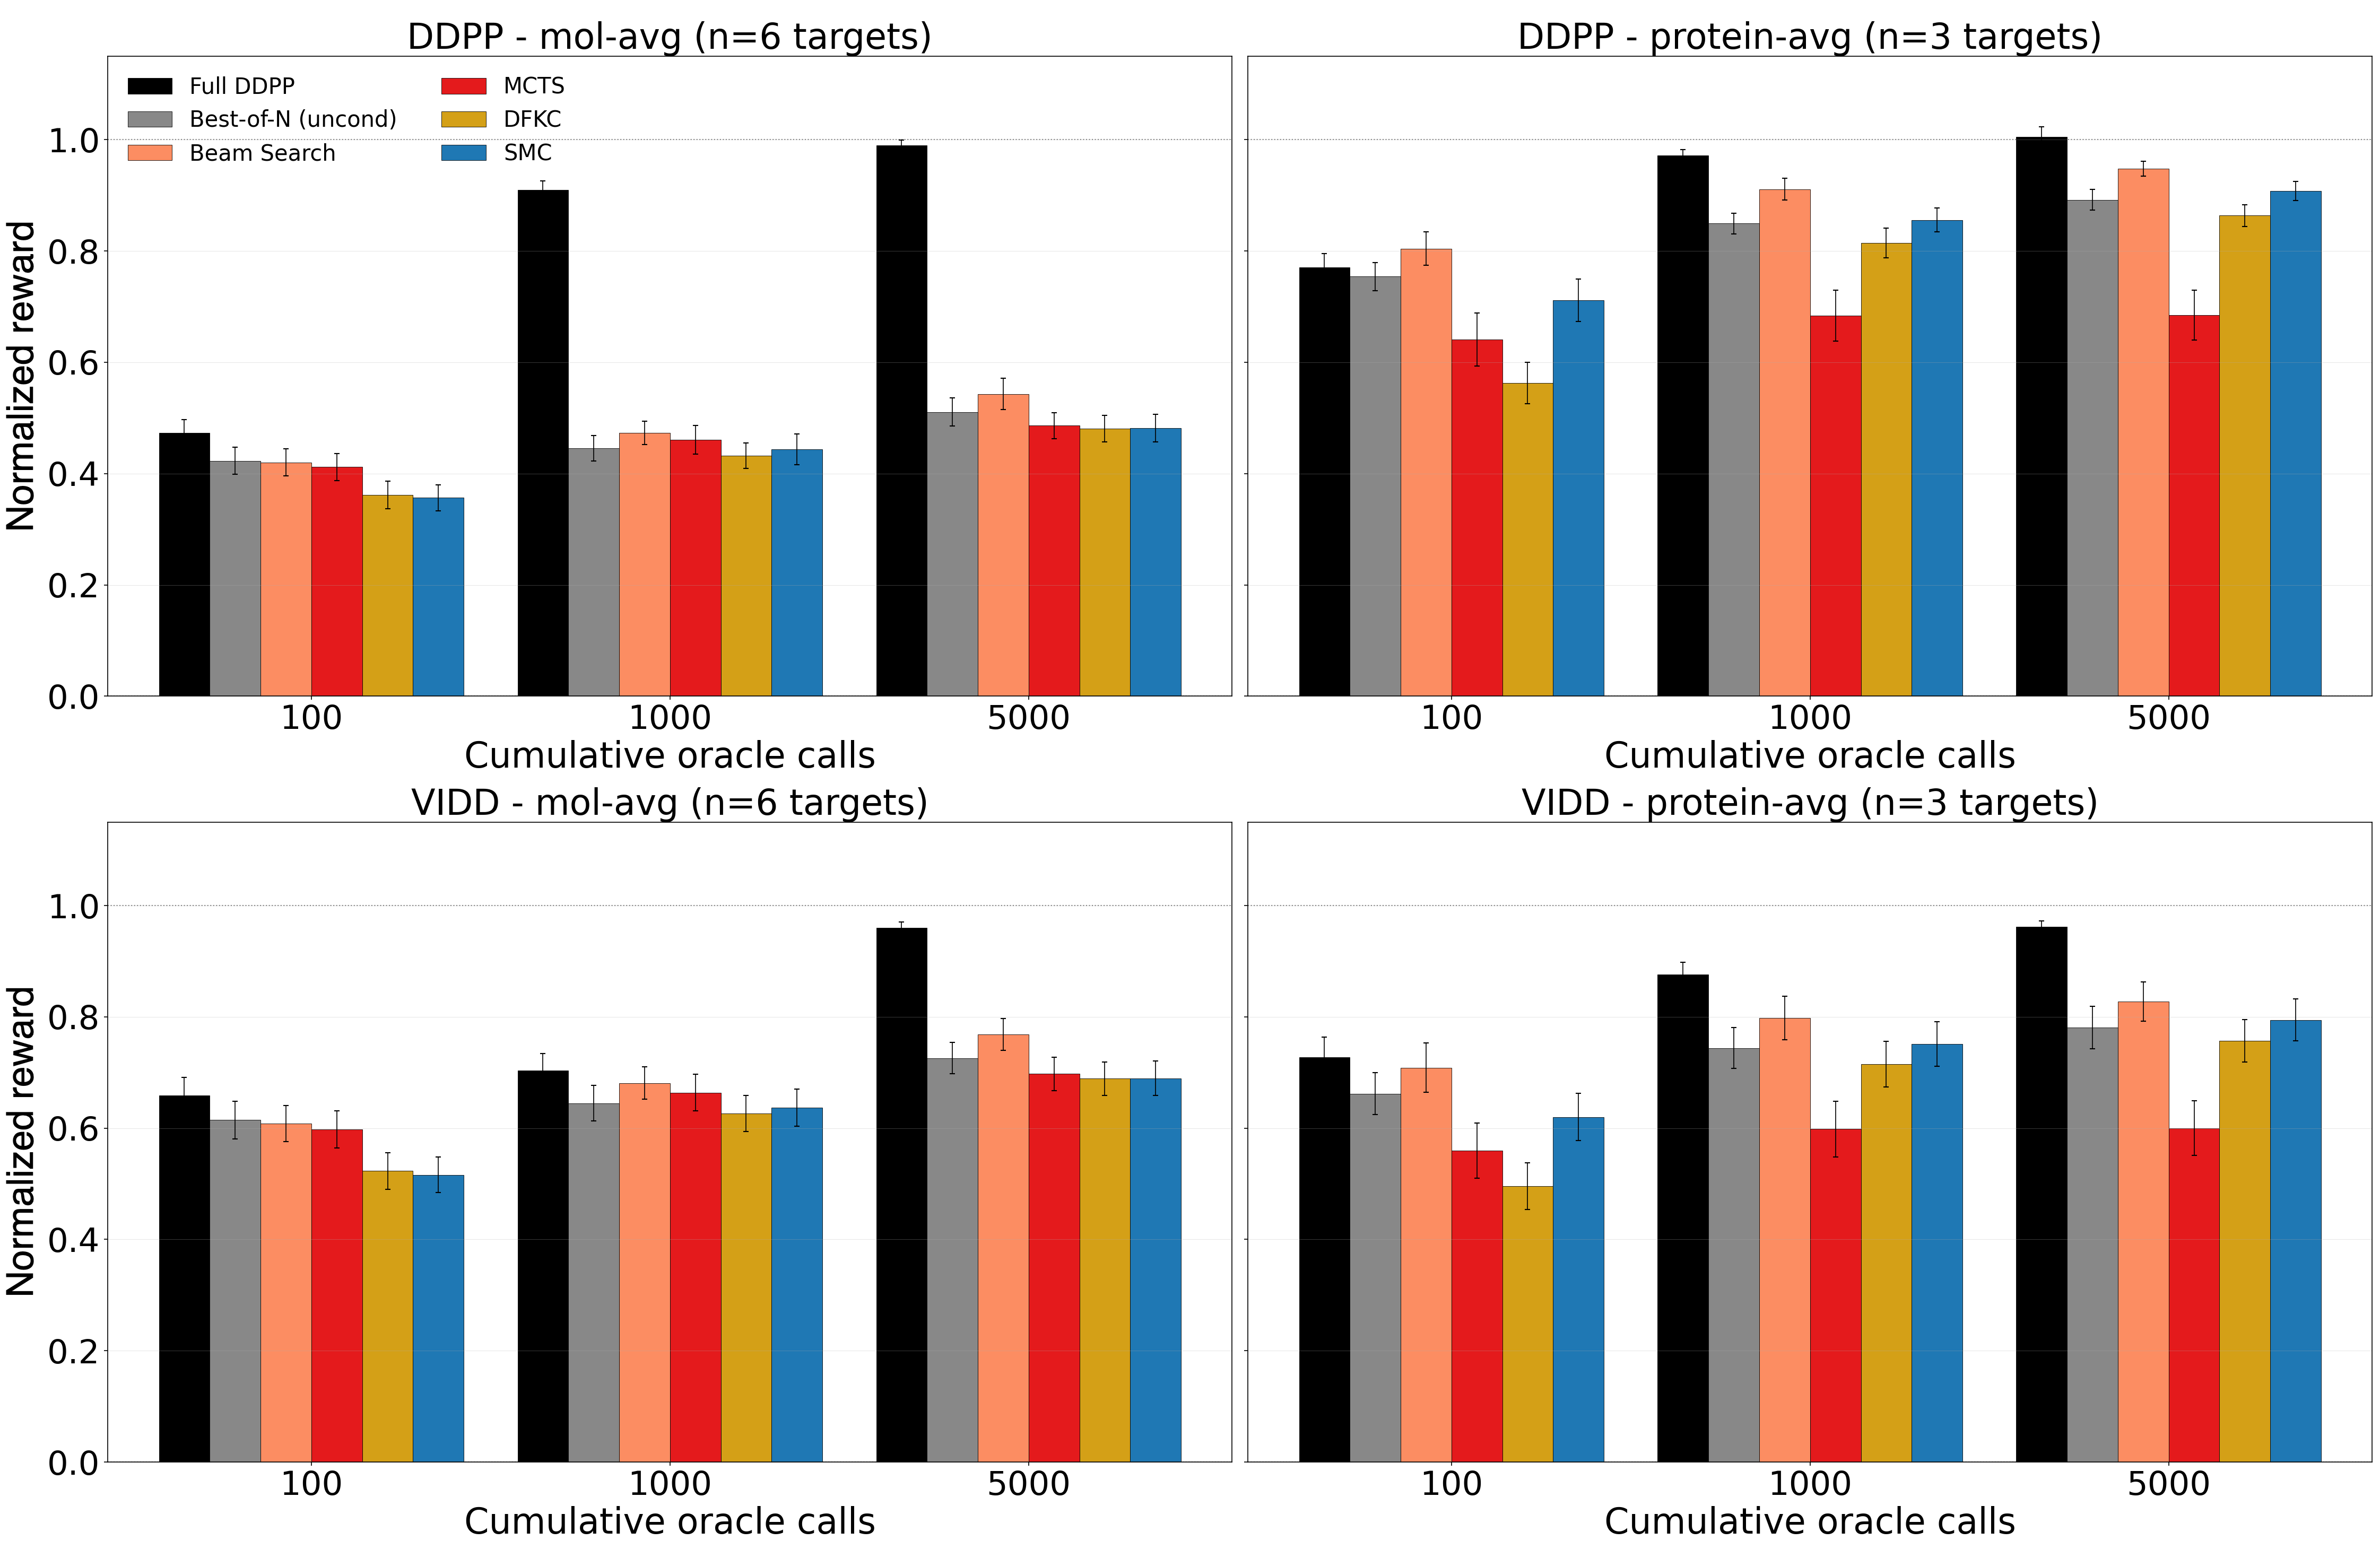
\includegraphics[width=0.90\textwidth]{figures/ablations/result2_combined_vs_search_1.png}
  % \vspace{-0.2in} % disabled to restore figure spacing
  \caption{\textbf{Online adaptation outperforms inference-time search most clearly on small-molecule tasks.} Full loop (black) versus five search baselines at matched oracle-call budgets. Protein terminal gaps are smaller despite a $16\times$ call-efficiency gain. Error bars: $\pm1$ SEM over target--seed runs; normalised reward per Eq.~\ref{eq:lift}.}
% Previous full caption retained for recovery.
% \caption{\textbf{Online adaptation outperforms inference-time search most clearly on small-molecule tasks.} Full loop (black) vs. five search baselines at 100/1k/5k calls, over molecule targets (left) and protein families (right). Note that modest terminal bar gaps on proteins coexist with a $16\times$ oracle speedup because bars compare scores at fixed budgets while speedup compares budgets to reach a fixed score (e.g., on TrpB, the full loop reaches beam search's $9{,}424$-call score of $1.666$ in just $738$ calls, a $12.8\times$ reduction despite a $0.026$ terminal difference at $10\text{k}$ calls). Error bars: ±1 SEM over (target, seed); normalised reward per Eq.~\ref{eq:lift}.}
  \label{fig:barplot_inference_search}
  % \vspace{-0.1in} % disabled to restore figure spacing
\end{figure}
% \vspace{-0.1in} % disabled to restore paragraph spacing
\textbf{Online Adaptation Outperforms Inference-Time Search.} 
Fig.~\ref{fig:barplot_inference_search} compares the full online harness against inference-time search baselines that keep the generator fixed during selection (best-of-$N$, beam, MCTS, DFKC, and SMC). The full loop dominates these baselines on small-molecule tasks because oracle feedback is reused through model updates rather than spent only on one-shot candidate selection. Averaged across the six small-molecule targets, the harness reaches the best search baseline's final score in $\approx 58\times$ fewer oracle calls; on protein-fitness tasks the corresponding speedup is $\approx 16\times$. Replacing DDPP-LB with VIDD as $\mathcal{L}_{\text{ft}}$ gives similar trends (Appendix~\ref{app:vidd-ablation}). 
Mechanistically, the advantage of online adaptation stems from resolving both the distributional and computational bottlenecks. Distributionally, inference-time search relies on lookahead rollouts or noisy discrete Tweedie estimates (Appendix Fig.~\ref{fig:tweedie_search}) to filter trajectories from a frozen prior $p_{\text{pre}}$; when high-affinity ligands reside far outside the prior's dominant modes, reweighting static samples cannot traverse the density gap, whereas gradient updates progressively shift the proposal distribution $p_{\theta_t}$ toward the high-reward basin. Computationally, while pure search discards feedback after each selection step, online adaptation amortizes each oracle query into persistent parameter updates, maintaining its advantage across $100\times$ oracle-cost rescalings and full Boltz-2 evaluations (Appendix Fig.~\ref{fig:boltz_surrogate}, Fig.~\ref{fig:boltz_oracle_1x}, Fig.~\ref{fig:oracle_rescale}).


%This speedup and the normalized-reward panels answer different questions, which is why a large speedup can coexist with a modest-looking bar. The normalised reward reads a budget-versus-score table \emph{down a column}: fix an oracle budget and compare scores, so a small terminal gap produces a small bar. The speedup reads the same table \emph{across a row}: fix a score and compare the budgets each method needed to reach it. On TrpB, for example, beam search ends at $1.666$ after $9{,}424$ calls while the full loop passes that score at $738$ calls, a $12.8\times$ gap, even though the two differ by only $0.026$ at the $10{,}000$-call budget. We keep normalised reward as the primary metric because the design objective is budgeted discovery, but the speedup is the more faithful summary of feedback efficiency. %Fig.~\ref{fig:barplot_inference_search} shows that the \textit{full method} of online adaptation outperforms baselines where only inference-time search methods (best-of-$N$, beam, MCTS, DFKC, SMC) are used (task-separated results in Fig.~\ref{fig:ablation_search}). Averaged across the six small molecules, the harness reaches the best search baseline's final score in $\approx 58\times$ fewer oracle calls; on the protein-fitness tasks the corresponding speedup is $\approx 16\times$.  Substituting VIDD for DDPP-LB as \mathcal{L}_{\text{ft}}$ results in similar trends (Appendix~\ref{app:vidd-ablation}).

\subsection{Understanding performance improvements through distribution shifts in \texorpdfstring{$p_{\theta_t}$}{p\_theta\_t}}\label{sec:analysis}
\begin{figure}[H]
  \centering
  % \vspace{-0.10in} % disabled to restore figure spacing
  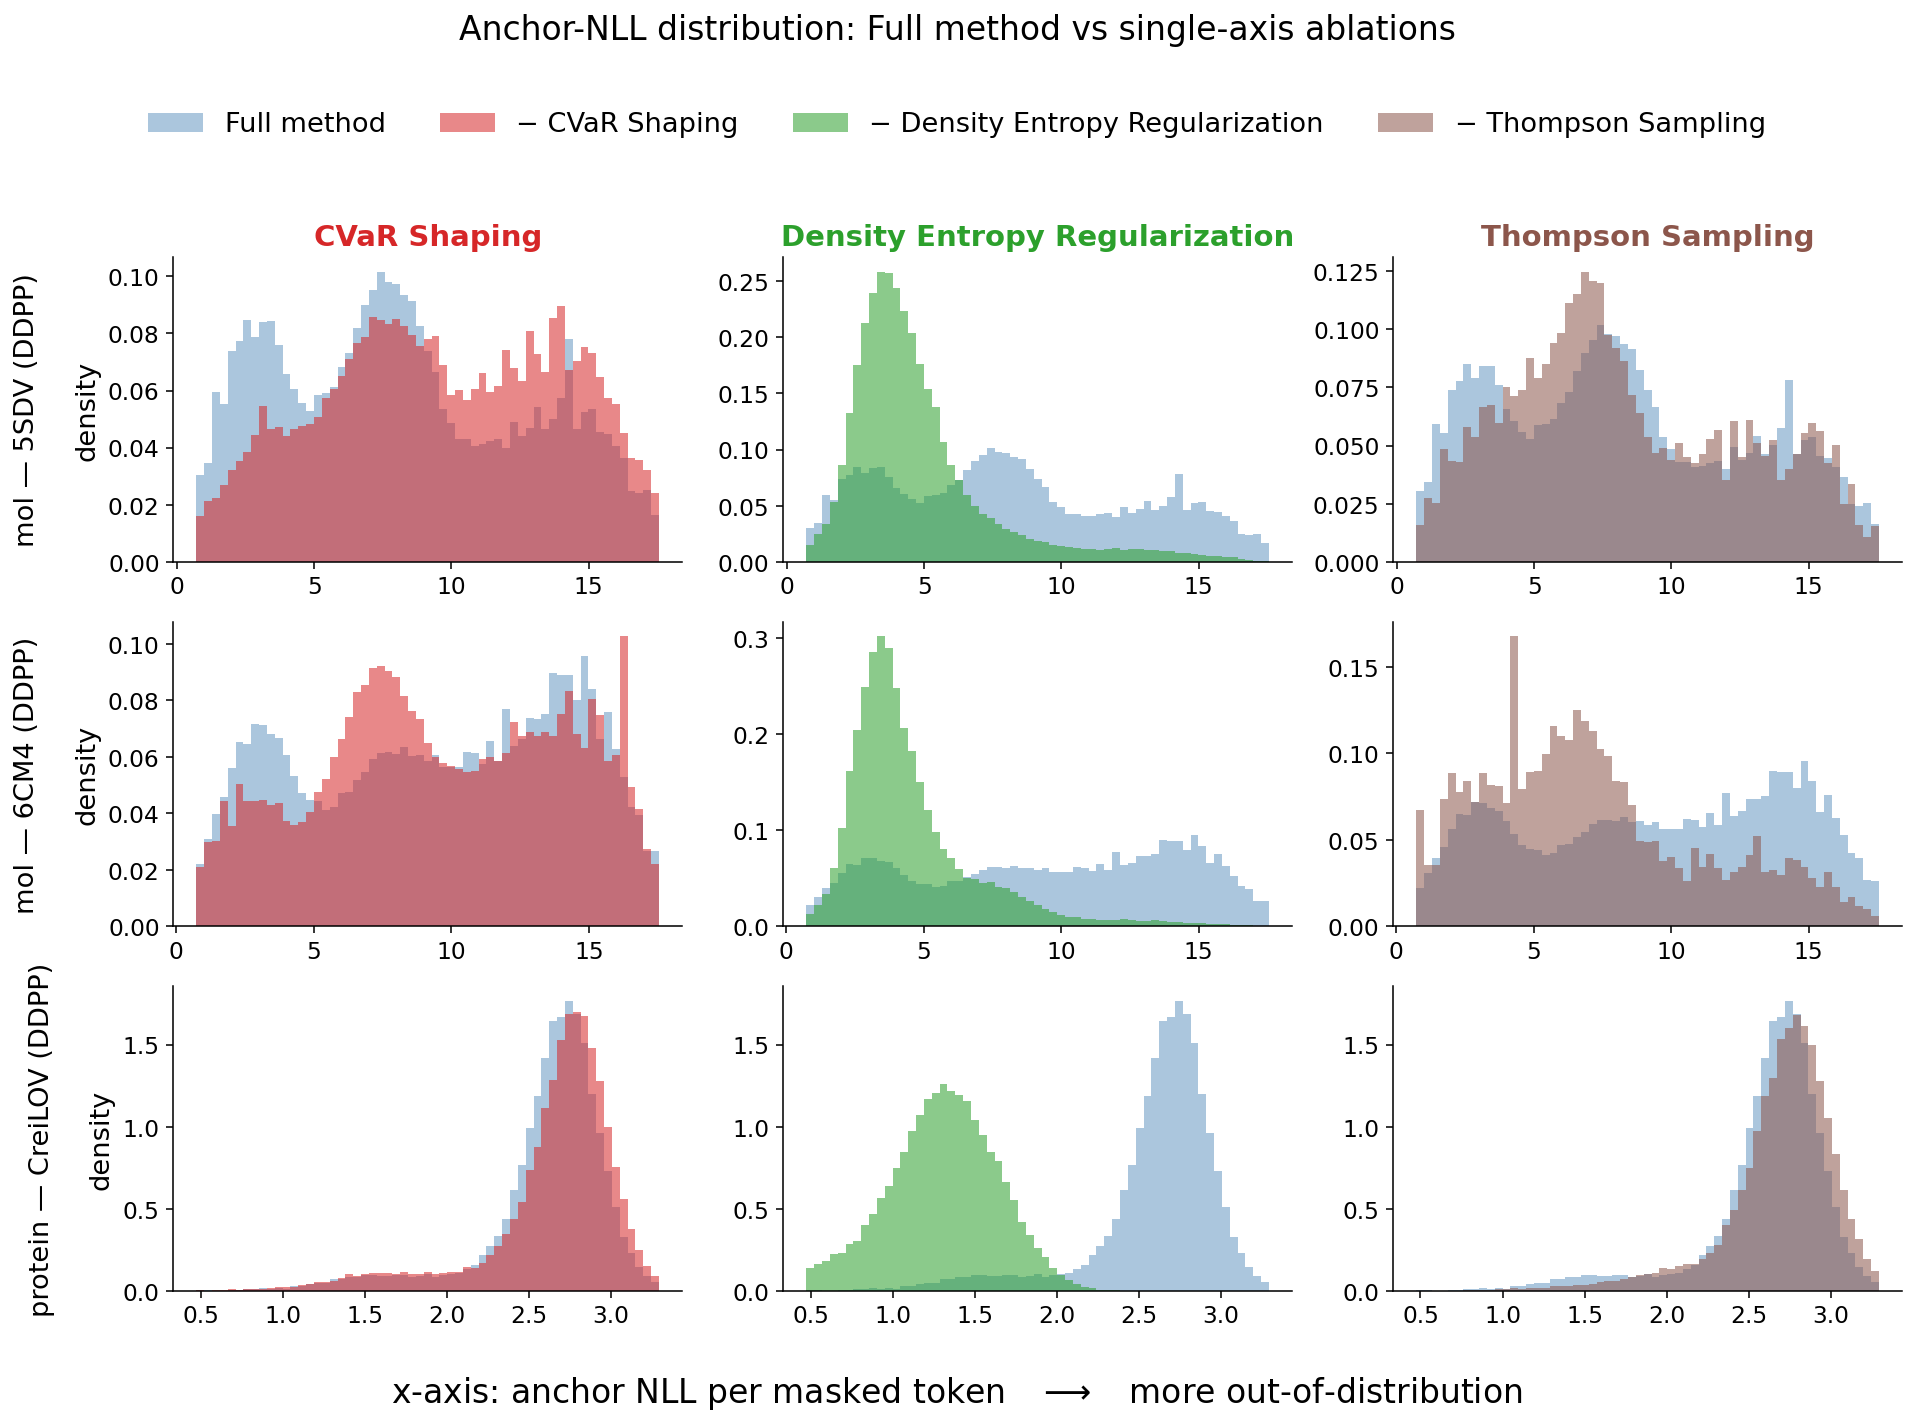
\includegraphics[width=0.90\textwidth]{figures_source/combined_NLL.png}
    % \vspace{-0.21in} % disabled to restore figure spacing
  \caption{\textbf{Distribution shifts in $p_{\theta_t}$ explain performance gains.} Run-end anchor-NLL for the full method versus leave-one-out ablations. Density Entropy Regularization produces the strongest off-prior shift, while protein shifts are weaker. Additional 2VT4R results appear in Appendix Fig.~\ref{fig:anchor_nll}.}
% Previous full caption retained for recovery.
% \caption{\textbf{Distribution shifts in $p_{\theta_t}$ explain performance gains for methods on tasks where high-reward molecular design solutions lie outside the original generative prior $p_{\theta_t}$.} Each panel overlays the run-end anchor-NLL density of the \emph{full method} (blue) against the corresponding leave-one-out \emph{ablation cell}; the x-axis ($-\log p_{\text{pre}}(x)$) measures how far each sample lies from the original generative prior. Density Entropy Regularization pushes mass away from the prior $p_{\theta_t}$. Overall, protein tasks experience weaker distribution shifts in $p_{\theta_t}$. Results for the additional small-molecule target 2VT4R are provided in Appendix Fig.~\ref{fig:anchor_nll}.}
  \label{fig:distribtuion_shift_main}
  % \vspace{-0.1in} % disabled to restore figure spacing
\end{figure}


The domain dependence in Fig.~\ref{fig:barplot_ablation} is largely explained by how far adaptation must move the generator away from its pretrained prior. Fig.~\ref{fig:distribtuion_shift_main} measures this shift using anchor NLL under the frozen pretrained model, $-\log p_{\text{pre}}(x)$. Density Entropy Regularization has the strongest and most direct effect on this distribution: removing it collapses mass back toward high-density regions of the pretrained prior. This matches its role in the objective, where the likelihood penalty discourages repeatedly reinforcing modes the current generator already occupies.
%Understanding why individual components complement each other largely boils down to how distribution shifts are handled. We study the effects in Fig.~\ref{fig:distribtuion_shift_main}.  Our main findings here are that: (1) Entropy regularization has a strong effect on the distribution shape, pushing the generator to produce more out-of-distribution samples. (2) Thompson sampling and CVaR shaping sometimes pull the generator more out-of-distribution, and sometimes less, showing that the a priori likelihood of high-reward regions are task-dependent. (3) The generating distribution for protein diffusion models are significantly less effected by CVaR shaping and Thompson sampling, providing evidence that the prior distribution already captures high-reward regions.

CVaR shaping and Thompson sampling affect distribution shift more conditionally. CVaR focuses the gradient on the upper reward tail, while Thompson sampling changes which uncertain candidates receive oracle calls. Either mechanism can move the generator farther from the prior when high-reward candidates lie in low-density regions, but neither has a fixed direction of shift. In Fig.~\ref{fig:distribtuion_shift_main}, the no-CVaR and full-method densities nearly overlap on protein-CreiLOV, where the prior already appears to cover the high-reward basin. On small-molecule targets such as 5SDV and 6CM4, removing CVaR or Thompson produces a visible change in the high-NLL tail, indicating that reward shaping and acquisition can help expose off-prior high-reward regions.
%CVaR shaping and Thompson sampling affect distribution shift more conditionally. CVaR focuses the gradient on the upper reward tail, while Thompson sampling changes which uncertain candidates receive oracle calls. Either mechanism can move the generator farther from the prior when high-reward candidates lie in low-density regions, but neither has a fixed direction of shift. In Fig.~\ref{fig:distribtuion_shift_main}, the no-CVaR and full-method densities nearly overlap on protein-CreiLOV, where the prior already appears to cover the high-reward basin. On small-molecule targets such as 5SDV and 6CM4, removing CVaR or Thompson produces a visible change in the high-NLL tail, indicating that reward shaping and acquisition can help expose off-prior high-reward regions.
%The three adaptation strategies (CVaR, Density Entropy Regularization, Thompson) act on the search in complementary ways: CVaR concentrates gradient on the upper tail, debiasing redistributes it off occupied modes, and Thompson diversifies which uncertain candidates pay an oracle call. While Density Entropy Regularization is by definition off-prior, Thompson sampling and CVaR shaping do not have a fixed sign of distribution shift. Depending on whether the high-reward region is already well-covered by the prior, they pull the generator more or less out-of-distribution. This is visible directly in Fig.~\ref{fig:distribtuion_shift_main}: the no-CVaR and full-method densities overlap almost exactly on protein-CreiLOV (where the prior already covers the high-reward mutant basin), while on mol-5SDV / mol-6CM4 removing CVaR or Thompson produces a small but visible drift in the high-NLL tail.

Once acquisition and reward shaping move $p_{\theta_t}$ into less prior-dense regions, the main failure mode shifts from insufficient exploration to target mismatch. A naive on-policy update trains only on the current batch, so earlier high-reward discoveries can stop influencing the generator. The replay buffer addresses this by aligning the gradient with the reward-tilted distribution over all evaluated data, not just the latest on-policy samples. A second mismatch appears when reward optimization moves probability mass off the valid molecular manifold. The invalid-SMILES penalty gives these failures a low-reward training signal, pulling $p_{\theta_t}$ back whenever exploration produces invalid strings. These components are therefore best understood as guardrails for the exploratory loop rather than as the main drivers of distribution shift.
%Once the shaping and acquisition components move $p_{\theta_t}$ into high-reward off-prior regimes, the main failure mode comes from not maintaining the right optimization target. A naive on-policy update discards historical data and pushes probability mass onto invalid-SMILES strings the penalty would have blocked. The two objective-mismatch corrections handle these failures separately. The buffer aligns the gradient with the reward-tilted posterior over all evaluated data, not just the current batch. The invalid-SMILES penalty pulls $p_{\theta_t}$ back whenever a sample lands off the SAFE manifold. Removing any single knob degrades one or more of the following metrics (top-1, top-10\%, or validity) (Fig. ~\ref{fig:barplot_ablation}. Against the strongest pure-search and normal online-finetuning baselines, the full assembled stack dominates under matched compute on the FA oracle (Appendix Fig.~\ref{fig:final_comparison}).

This distributional view explains why the ablation effects are stronger on small-molecule tasks and weaker on protein-fitness tasks. The small-molecule generator is a broader prior, so high-affinity candidates often require larger shifts away from its dominant modes. The protein generators are family-specific, so high-fitness variants appear closer to regions already covered by the pretrained prior. As a result, reward shaping and debiasing are less decisive on proteins, while acquisition can still help by allocating oracle calls more effectively. This also explains why search baselines and ablations converge more quickly on the protein tasks: when the prior already places mass near high-reward modes, adapting the generator and selecting from it become closer in effect.
%Fig.~\ref{fig:barplot_ablation} and Fig.~\ref{fig:barplot_inference_search} show that performance for protein tasks is less sensitive to design components than that of small-molecule tasks. An explanation is that proteins with high rewards lie more within distribution $p_{\theta_t}$, compared to molecules. We attribute this to the fact that optimal protein with high fitness is far more in-domain relative to its generative prior than the molecule with high binding affinity is to its prior. This is further evidenced by the fact that search baselines and ablations quickly converge to similar final scores because the prior already concentrates on the high-reward modes. x



\section{Conclusion}
This work studies how to use limited oracle feedback for molecular optimization with pretrained discrete diffusion models. Our main finding is that online adaptation benefits from combining components that act on different parts of the feedback loop. Acquisition, CVaR reward shaping, and Density Entropy Regularization provide the clearest reward gains on small-molecule tasks, while replay and invalid-output penalties stabilize the exploratory loop. Together, these components form a practical recipe that outperforms offline fine-tuning and inference-time search baselines under matched oracle-call budgets and GPU-hour accounting.

The results also clarify when this recipe is most useful. Small-molecule binding optimization often requires moving beyond high-density regions of a broad pretrained prior, so shaping and debiasing matter more. Protein-fitness tasks show weaker ablation effects, consistent with family-specific priors already covering high-fitness regions more closely; in that regime, acquisition remains useful because oracle-call allocation still matters, but large distribution shifts are less central. Future work should extend this recipe to settings with less reliable learned oracles, multi-objective design goals, and other discrete-generation domains with non-differentiable feedback. %The methods are dual-use in principle, but our experiments use standard binding-affinity and protein-fitness oracles and do not introduce harmful-property predictors.

\textbf{Limitations.} We treat the oracle as a faithful proxy for the property of interest, but aggressively optimizing learned oracles can exploit their biases rather than produce candidates that transfer to wet-lab validation. We also optimize a single scalar reward, whereas realistic molecular design is multi-objective and often seeks a Pareto frontier over potency, ADMET, synthesizability, novelty, and IP. Finally, we study biological design tasks with biology-style oracles; the same recipe may transfer to other discrete-generation domains with non-differentiable oracles, but we do not demonstrate that empirically. The methods are dual-use in principle, though our experiments use standard binding-affinity and protein-fitness oracles and do not introduce harmful-property predictors.

\begin{ack}
This work was primarily conducted by researchers at Caltech, who were supported in part by NSF \#2505096, and gifts from Genesis Therapeutics, Point72, and OpenAI. Jason Yang was supported in part by a Google Fellowship. Riccardo De Santi was supported by an ETH AI Center doctoral fellowship, the Swiss
National Science Foundation under NCCR Catalysis (grants 180544 \& 225147) and NCCR Automation (grant 51NF40 180545), and Centres of Competence in Research funded by the Swiss National Science Foundation.

\textbf{Competing interests.} Nate Gruver, Pranav Murugan, Alexander F.~G.~Goldberg, and Maruan Al-Shedivat are affiliated with Genesis Molecular AI.
\end{ack}

%This work studies how to efficiently allocate expensive evaluation resources in molecular optimization using generative models. We found that an online active finetuning loop combining CVaR upper-tail reweighting, model debiasing, Thompson sampling over an ensemble surrogate, a replay buffer, and an invalid penalty consistently dominates pure-search and untreated-online-finetuning baselines. Interestingly, the benefits are more pronounced when high-reward solutions lie further out of distribution, such as in the case of small molecule tasks, compared to the protein tasks studied here. This is likely explained by the fact that the generator for the small molecule, GenMol, is more general, whereas the generators used for protein tasks are trained on specific protein families, and therefore less exploration is required.


%Several limitations bound the scope of these claims. First, we treat the  oracle as a faithful proxy for the property of interest.  Aggressively optimizing such oracles may simply be exploiting their biases, leading to less effective wet lab experiments. Second, every run optimizes a single scalar reward, while realistic molecular design is multi-objective (potency must be balanced against ADMET, synthesizability, novelty, and IP) and the right answer is typically a Pareto frontier rather than a single best molecule; extending the recipe to multi-objective rewards is straightforward in principle but not evaluated here. Third, both task families we study are biology problems with biology-style oracles, so although the recipe only requires a discrete-diffusion prior and a non-differentiable oracle and should transfer to other discrete-generation domains (materials, code, structured combinatorial design), we do not demonstrate that transfer empirically.


%Several limitations bound the scope of these claims. We treat the oracle as a faithful proxy for the property of interest, but aggressively optimizing learned oracles can exploit their biases rather than produce candidates that transfer to wet-lab validation. We also optimize a single scalar reward, whereas realistic molecular design is multi-objective and often seeks a Pareto frontier over potency, ADMET, synthesizability, novelty, and IP. Finally, we study biological design tasks with biology-style oracles; the same recipe may transfer to other discrete-generation domains with non-differentiable oracles, but we do not demonstrate that empirically. The methods are dual-use in principle, though our experiments use standard binding-affinity and protein-fitness oracles and do not introduce harmful-property predictors.

%The same machinery could in principle be pointed at oracles that score for harmful molecules; we view this as a low marginal risk because (i) the bottleneck in producing such molecules is the oracle and the wet-lab synthesis, not the generative model, and (ii) the techniques we describe (CVaR shaping, model debiasing, Thompson sampling, replay buffer, invalid-output penalty) are generic active-learning patterns and not tied to any specific dangerous property predictor. %We do not release any oracle for harmful properties. We use only public, established binding-affinity oracles (FA, Boltz-2) on standard PDB targets, and the small-molecule outputs are at most candidate hypotheses that would still require independent evaluation before any wet-lab synthesis.

\newpage

\bibliographystyle{unsrtnat}
\bibliography{main}

%%%%%%%%%%%%%%%%%%%%%%%%%%%%%%%%%%%%%%%%%%%%%%%%%%%%%%%%%%%%

\newpage

\appendix

\section*{Guide to the Appendix}
The appendix follows the logic of the paper: definitions and reproducibility first, then method illustrations, controlled component evidence, search comparisons, task-level results, and finally the alternative-oracle and qualitative checks.
\begin{itemize}
\item \textbf{Experimental definitions and reproducibility (Appendix~\ref{app:method-details}).} Normalization, budget accounting, backbones and oracles, implementation details, hyperparameters, the reproduction recipe, and stochasticity.
\item \textbf{Method and baseline illustrations (Appendix~\ref{app:diagrams}).} The active loop, fine-tuning and exploration components, inference-time search families, and computational shortcuts.
\item \textbf{Component ablations and diagnostics (Appendix~\ref{app:component-analysis}).} Individual knobs, secondary metrics, distribution-shift diagnostics, the joint factorial, the untreated baseline, and cross-finetuner results.
\item \textbf{Search baselines and compute accounting (Appendix~\ref{app:search}).} Online versus offline adaptation, frozen-generator search, search inside the online loop, and oracle-cost sensitivity.
\item \textbf{Task-level and aggregate results (Appendix~\ref{app:results-detail}).} Per-task curves, domain aggregates, GPU-hour views, and pointers to the canonical main-text bar plots.
\item \textbf{Alternative oracle and qualitative examples (Appendix~\ref{app:external-validation}).} Boltz-2 experiments and representative valid molecules.
\end{itemize}

% Previous appendix guide retained for recovery.
% \section*{Guide to the Appendix}
% The appendix is organized around the questions addressed by the main experiments. Use the guide below to locate the corresponding evidence and implementation details.
% \begin{itemize}
% \item \textbf{Implementation and reproduction.} Appendix~\ref{app:method-details} defines normalization and compute accounting, documents the backbones and oracles, and gives hyperparameters and a reproduction recipe. Appendix~\ref{app:diagrams} illustrates the active loop, its components, and search baselines.
% \item \textbf{Do the components help individually and jointly?} Appendix~\ref{app:knobs} collects controlled single-component experiments and diagnostics. Appendix~\ref{app:factorial} gives the three-component factorial and the all-five-knobs-off comparison. Appendix~\ref{app:vidd-ablation} provides the DDPP-LB/VIDD numerical summary and VIDD trajectories.
% \item \textbf{How does adaptation compare with search?} Appendix~\ref{app:search} groups online/offline comparisons, search shortcuts, online search hybrids, and compute-cost sensitivity.
% \item \textbf{Where do effects vary across tasks and budgets?} Appendix~\ref{app:per-task-ablation} shows per-task oracle-call curves; Appendix~\ref{app:avg-ablation} aggregates them by domain; Appendix~\ref{app:gpuhrs-ablation} gives the GPU-hour counterparts. Appendix~\ref{app:per-target-grids} points to the canonical main-text bar plots.
% \item \textbf{Additional diagnostics and oracle.} Appendix~\ref{app:traces} reports validity, diversity, QED, SA, and anchor-NLL diagnostics. Appendix~\ref{app:boltz} reports experiments using the Boltz-2 oracle. Valid molecule examples follow those results.
% \end{itemize}

\clearpage

% Previous heading: \section{Method Details}\label{app:method-details}
\section{Experimental Definitions and Reproducibility}\label{app:method-details}

This appendix records implementation specifics that are not stated in the main body. Hyperparameter values are collected in Table~\ref{tab:hparams}.

\subsection{Normalised Reward}\label{app:lift-fraction}

The normalised reward is defined in Eq.~\ref{eq:lift} in Sec.~\ref{sec:exp-setup}. The target-specific endpoints $C_t$ and $F_t$ are computed over the figure-specific method set: component ablations together with \texttt{best\_of\_n} for Fig.~\ref{fig:barplot_ablation}, and the full configuration together with search baselines for Fig.~\ref{fig:barplot_inference_search}. Per-bar means and symmetric SEMs are pooled over target--seed draws.

% Previous appendix definition retained for recovery after moving the equation to the main text.
% \subsection{Normalised Reward}\label{app:lift-fraction}
% 
% Across the bar plots in Sec.~\ref{sec:results} and the appendix grids we report a per-target normalised reward, rescaling each target's scores to a common [0, 1] range.
% \begin{equation}
% \mathrm{lift}_t(x) \;=\; \frac{r_t(x) - C_t}{F_t - C_t},
% \label{eq:lift}
% \end{equation}
% where $r_t(x)$ is the score of method $x$ on target $t$ at a given slice, and $C_t$ / $F_t$ are the per-target $\min$ at call=1 and $\max$ at the run end, taken over a figure-specific method set: knobs $\cup$ \texttt{best\_of\_n} for Fig.~\ref{fig:barplot_ablation}, full method $\cup$ search baselines for Fig.~\ref{fig:barplot_inference_search}. Per-bar mean and symmetric SEM are pooled over (target, seed) draws of $\mathrm{lift}_t$.
% 
% 
\subsection{Wall-time accounting}

Wall time for a single run decomposes as
\begin{equation}
t_{\text{wall}} \;=\; N \cdot c_{\text{oracle}} + C_{\text{method}},
\label{eq:wall-decomp}
\end{equation}
where $N$ is the number of oracle calls, $c_{\text{oracle}}$ is the per-call oracle cost, and $C_{\text{method}}$ collects all method-side compute (generation, fine-tuning steps, surrogate updates). Reporting against both axes (oracle calls and GPU hours) reveals whether one technique dominates another regardless of oracle cost, or only past a threshold $c_{\text{oracle}}^\star$ at which the two curves cross. The retroactive $100\times$ oracle-cost rescaling used throughout the appendix figures simulates a switch from a fast oracle (FA) to a slow oracle (Boltz-2-class) by scaling $c_{\text{oracle}}$ in this decomposition without re-running the experiments.


\subsection{Backbone and oracle internals}

The GenMol checkpoint we use is the released MDLM-style masked discrete diffusion model over SAFE-tokenized SMILES \citep{noutahiGottaBeSAFE2023, sahoo2024mdlm} with vocabulary size 1882 (1880 SAFE tokens plus mask and end-of-sequence). The forward noise schedule and architecture are unchanged from the release; only the policy weights $\theta$ are updated. A FlashAffinity call decomposes as: parse the SMILES with RDKit; embed a 3D conformer with ETKDGv3 (one retry on failure); extract per-atom features with the FA torchdrug parser; score the (pocket, ligand) pair with the released FA checkpoint. Per-pocket ESM3 protein features are pre-computed once and cached. Each FA call takes tens of milliseconds on the A100; Boltz-2 calls take roughly $20$ seconds on the same hardware, two orders of magnitude slower.

\subsection{Run logs}

The compute-breakdown plots (Appendix Figs.~\ref{fig:search_overhead} and~\ref{fig:compute_breakdown}) and the retroactive $100\times$ oracle-cost rescaling are computed offline from two log files written during every run. \texttt{oracle\_timeline.jsonl} has one line per oracle call (cumulative call count, SMILES, score, best-so-far, elapsed seconds, RDKit-derived QED and SA, epoch index). \texttt{active\_loop\_log.jsonl} has one line per active-loop round (round number, top-1 best-so-far $f^\star$, mean ensemble disagreement $\sigma$, Spearman $\rho$ between ensemble and oracle on a held-out $20\%$ of the buffer, cumulative wall seconds, and per-phase wall times $t_{\text{gen}}, t_{\text{surrogate}}, t_{\text{oracle}}, t_{\text{ddpp}}, t_{\text{ensemble}}$).

\subsection{Implementation subtleties}

Three details are not derivable from Algorithm~\ref{alg:method} or Table~\ref{tab:hparams} and matter for reproducing our numbers.

\paragraph{Gradient detach in model debiasing.} $\log p_\theta(x)$ in Eq.~\ref{eq:debias} is treated as a constant: gradient is not propagated through the debiasing term. Passing gradient through it turns the loss into an entropy-regularized policy gradient and breaks the posterior-matching guarantee of DDPP-LB.

\paragraph{Thompson noise scope.} At acquisition we draw one $\varepsilon \sim \mathcal{N}(0, 1)$ per candidate, shared across all $J$ ensemble heads, not one per (candidate, head) pair. The per-candidate scalar acts on the ensemble disagreement $\sigma_i$ and is what produces the diversity push described in Sec.~\ref{sec:results}.

\paragraph{CVaR threshold refresh.} The threshold $\tau$ is recomputed once per active-loop epoch from the empirical $q$-quantile of buffer rewards, not per gradient step. Below-threshold samples remain in the gradient with their shaped reward floored at $\epsilon = 10^{-8}$, which under the DDPP log-reward becomes a strong negative signal that pushes $q_\theta$ away from them rather than dropping them entirely.

\subsection{Hyperparameters}

Table~\ref{tab:hparams} lists the hyperparameter values used throughout the controlled experiments and the final-comparison runs. Defaults follow the recommended settings from the original DDPP-LB and VIDD references where applicable; values for the active-loop wrappers ($M, K, G$, ensemble size and training schedule) follow our active-loop reference implementation. We did not run an exhaustive per-method hyperparameter sweep. The design space we ablate has thirteen-plus methods (Table~\ref{tab:methods}) crossed with five seeds and a two-hour FA budget per cell, and the cost grows by another order of magnitude under the Boltz-2 oracle; tuning each cell independently would multiply that cost by the size of the per-method search grid and would also confound the design-space comparison, since improvements would no longer be attributable to the knob under study versus to a more aggressive sweep on one cell than another. We instead control everything except the knob being ablated, hold all other hyperparameters at the active-loop reference defaults, and run every cell at the same wall budget. The trade-off is explicit: we measure the effect of each design choice at sensible-default settings rather than at each method's peak-tuned setting. Per-knob sensitivity to the hyperparameter most likely to matter (the invalid-SMILES penalty magnitude) is reported separately in Appendix Fig.~\ref{fig:penalty_sweep}.

\begin{table}[H]
\centering
\small
\begin{tabular}{@{}l l l@{}}
\toprule
\textbf{Group} & \textbf{Hyperparameter} & \textbf{Value} \\
\midrule
\multicolumn{3}{@{}l}{\textit{Wall budget and seeds}} \\
& Seeds                         & $\{0, 1, 2, 3, 42\}$ \\
& Wall budget per seed (FA)     & 2 hours \\
& Wall budget per seed (Boltz-2) & 10 hours \\
& Hardware                      & 1$\times$ NVIDIA A100 80GB \\
\midrule
\multicolumn{3}{@{}l}{\textit{Active loop}} \\
& Generation batch $M$          & 1000 \\
& Oracle batch $K$              & 25 \\
& Fine-tuning steps per round $G$ & 50 \\
& Buffer capacity               & 10\,000 \\
& Buffer eviction               & priority (lowest reward first) \\
& Fresh-fraction                & 0.25 \\
\midrule
\multicolumn{3}{@{}l}{\textit{Reward shaping}} \\
& CVaR quantile $q$             & 0.8 \\
& Reward floor                  & $10^{-8}$ \\
& Model-debiasing weight $\gamma$ & 1.0 \\
& Invalid-SMILES penalty $r_{\text{inv}}$ & $-5$ \\
\midrule
\multicolumn{3}{@{}l}{\textit{Surrogate ensemble (Thompson)}} \\
& Ensemble size $J$             & 10 \\
& Hidden width                  & 256 \\
& Training epochs / round  & 100 \\
& Learning rate                 & $10^{-3}$ \\
& Mini-batch size               & 256 \\
\midrule
\multicolumn{3}{@{}l}{\textit{Fine-tuning (DDPP-LB)}} \\
& Backbone learning rate        & $5 \times 10^{-5}$ \\
& LogZ head learning rate       & $5 \times 10^{-4}$ \\
& EMA decay                     & 0.999 \\
& Backbone warmup (LogZ-only steps) & 200 \\
\midrule
\multicolumn{3}{@{}l}{\textit{Search baselines (when used as a knob)}} \\
& Beam: $N$ beams, $L$ branches, $K$ steps & $N{=}8$, $L{=}4$, $K{=}5$ \\
& MCTS: $c_{\text{UCT}}$, $L$, $K$         & $1.0$, $4$, $5$ \\
& DFKC: particles, $\beta$, score\_start   & 8, 2.0, 0.5 \\
\bottomrule
\end{tabular}
\caption{\textbf{Hyperparameters used across all reported experiments.} Values are the active-loop reference defaults; only the knob being ablated is varied within a comparison.}
\label{tab:hparams}
\end{table}

\begin{table}[H]
\centering
\small
\begin{tabular}{@{}llrr@{}}
\toprule
\textbf{Hyperparameter} & \textbf{Values tested} & \textbf{Best score} & \textbf{Top-100} \\
\midrule
Ensemble size $J$ & 3, 5, \textbf{10} & $0.20$ & $0.07$ \\
Invalid penalty $r_{\text{inv}}$ & 0, $-1$, $-3$, $\mathbf{-5}$, $-7$ & $0.36$ & $0.38$ \\
Buffer capacity & 100, 1000, \textbf{unlimited} & $0.13$ & $0.21$ \\
CVaR quantile $q$ & 0.60, 0.70, \textbf{0.80}, 0.90 & $0.14$ & $0.16$ \\
Oracle batch $K$ & 10, \textbf{25}, 50 & $0.25$ & $0.32$ \\
Debias weight $\gamma$ & 0.25, 0.5, \textbf{1.0}, 2.0 & $1.02$ & $1.01$ \\
\bottomrule
\end{tabular}
\caption{\textbf{Hyperparameter sensitivity.} Largest absolute change relative to the default (bold) in best score and top-$100$ mean, averaged over $3$ targets with $3$ runs per value per target. The sweep's default cell runs an unbounded buffer; this matches the $10{,}000$ capacity of Table~\ref{tab:hparams} in effect, because no run evaluates more than $8{,}750$ candidates, so the cap never binds and never evicts. The mean within-cell standard deviation is $0.22$, so the five small effects are of the same order as run-to-run variation. The debiasing weight is the exception, and it sets a threshold rather than requiring tuning: the score rises from $\gamma{=}0.25$ to $\gamma{=}1.0$ and does not rise further at $\gamma{=}2.0$, so any $\gamma \ge 1$ is equivalent --- consistent with $\gamma{=}1$ putting $\log r$ and $\log p_\theta$ on the same scale. $K$ is set by the ratio $K/M$ of oracle batch to generation batch rather than by tuning: performance is flat from $K{=}10$ to $K{=}25$ and drops at $K{=}50$, where the surrogate is barely filtering the pool.}
\label{tab:hpsens}
\end{table}

These sweeps do consume oracle calls. They were run on $3$ targets at $3$ seeds and were \emph{not} used to retune per-target settings: the configuration reported in Table~\ref{tab:hparams} is held fixed across all six molecular targets, all three protein families, and all seeds, so the reported results do not benefit from per-target tuning.


\subsection{End-to-end reproduction recipe}\label{app:repro-recipe}

This subsection lists, in order, every concrete asset and step required to reproduce one cell of our experimental table; combined with Algorithm~\ref{alg:method} (the abstract loop) and Table~\ref{tab:hparams} (the numerical settings), this is sufficient to rebuild the environment and re-run.

\paragraph{Software environment.} Python 3.10. PyTorch 2.x with CUDA 12.x. RDKit 2024.x (used for SAFE encoding/decoding, validity checking via \texttt{MolFromSmiles}, and ETKDGv3 conformer embedding). NumPy 1.x. Hydra for configuration. \textbf{boltz} package version 2.2.1 (PyPI) for the Boltz-2 oracle path.

\paragraph{Pretrained assets (downloaded once, cached locally).} (i) The \textbf{GenMol} masked discrete-diffusion checkpoint from \citet{leeGenMolDrugDiscovery2025} (ICML 2025; arXiv:2501.06158), released by the authors at \url{https://github.com/NVIDIA-BioNeMo/genmol}; we use the second-vocab-fix release shipped as \texttt{model\_v2.ckpt} (1397\,MB, vocabulary $1882$ = $1880$ SAFE tokens plus mask and end-of-sequence). Forward noise schedule and architecture are unchanged from the release; only the policy weights $\theta$ are updated. The model was pretrained on the \textbf{SAFE dataset V2} (\url{https://huggingface.co/datasets/datamol-io/safe-drugs}); we do not retrain. (ii) The \textbf{FlashAffinity} (FA) affinity-regression checkpoint
\texttt{FlashAffinity/checkpoints/value\_2.ckpt}
from \citet{jiangFlashAffinityBridgingAccuracySpeed},
together with its torchdrug-style featurizer; we use the regression
(value) head, apply the released molecular-weight correction,
and negate the corrected prediction. (iii) For Boltz-2 oracle runs, the released Boltz-2 weights downloaded via the \texttt{boltz} package's bootstrap (structure checkpoint \texttt{boltz2\_conf.ckpt} + affinity head \texttt{boltz2\_aff.ckpt}), \citet{passaro2025boltz2}. (iv) Per-pocket \textbf{ESM3} protein-feature tensors, computed once per PDB target and cached to disk (\texttt{FlashAffinity/data/protein\_test/repr/esm3.lmdb}) so that no oracle call recomputes them.

\paragraph{Per-target inputs.} Each PDB target (2VT4, 5SDV, 6CM4, 7BKC, 7C7M, 7YLL) contributes the receptor structure plus the binding-pocket specification used by the FA / Boltz-2 oracle. We use the publicly released coordinates without modification.

\paragraph{Seed handling.} A run is identified by \texttt{(method, target, seed)} with seed $\in \{0, 1, 2, 3, 42\}$. At process start the seed is propagated to: \texttt{torch.manual\_seed}, \texttt{torch.cuda.manual\_seed\_all}, \texttt{numpy.random.seed}, Python's built-in \texttt{random.seed}, and the RDKit conformer-embedding seed passed to \texttt{ETKDGv3}.

\paragraph{Per-cell launcher.} Each cell is dispatched by a single launcher that takes \texttt{(method, target, seed, wall\_budget\_sec)} as arguments. The launcher loads the GenMol checkpoint, attaches the configured component slots from Sec.~\ref{sec:design-space} (acquisition rule, reward-shape modifier, replay strategy, validity penalty, finetuning objective), opens the two log files described in App.~\ref{app:method-details} (\texttt{oracle\_timeline.jsonl} and \texttt{active\_loop\_log.jsonl}), and runs the loop in Algorithm~\ref{alg:method}.

\paragraph{Per-round step counts.} Each active-loop epoch generates $M{=}1000$ candidate molecules from the current $q_\theta$, scores them with the surrogate ensemble, picks the top-$K{=}25$ for oracle evaluation under Thompson sampling, evaluates them, pushes each $(x, r)$ pair into the buffer (with $r{=}r_{\text{inv}}$ for RDKit-failed candidates), refreshes the CVaR threshold $\tau$ from the buffer's current $q$-quantile, and runs $G{=}50$ DDPP-LB gradient steps on stratified mini-batches drawn from the buffer with fresh-fraction $0.25$. The ensemble surrogate is refit at the end of each epoch on all accumulated $(x, r)$ pairs for $100$ inner training epochs at learning rate $10^{-3}$ and mini-batch size $256$.

\paragraph{Wall-budget enforcement.} A monotonic clock is checked after each round. If the elapsed wall time exceeds the configured \texttt{wall\_budget\_sec} (2~h for FA, 10~h for Boltz-2; a $4$-h cap was applied to the small-molecule batch1 runs documented in our latest data drop), the loop terminates after writing one final \texttt{active\_loop\_log.jsonl} entry and a \texttt{results.json} summary. If the runner is killed externally, only the per-epoch and per-call log files are guaranteed to be flushed; the partial-summary case is described in App.~\ref{app:method-details}.

\paragraph{Output artifacts.} Every cell produces a directory \texttt{<TARGET>/<METHOD>\_s<SEED>/} containing exactly three files: \texttt{results.json} (post-run summary or partial stub), \texttt{active\_loop\_log.jsonl} (one JSON line per epoch), and \texttt{oracle\_timeline.jsonl} (one JSON line per oracle call). All paper figures are produced from these three file types alone; no additional artifacts are needed for plot regeneration.

\subsection{Sources of stochasticity beyond the seed}\label{app:stochasticity}

Setting the seed described above pins all explicitly-RNG-driven sampling decisions: which $M$ candidates the diffusion sampler draws each epoch, the Thompson noise $\varepsilon$ at acquisition, mini-batch composition during fine-tuning, ensemble weight initialization, and the conformer seed handed to RDKit. Several other sources of variation are \emph{not} pinned by the seed, and we list them here so that bit-level reproducibility is not expected even between two runs with identical \texttt{(method, target, seed)}.

\paragraph{GPU floating-point nondeterminism.} cuBLAS / cuDNN convolution and matmul algorithms make algorithm-selection decisions based on workspace memory and tensor shapes, and several reduction kernels (e.g., \texttt{scatter\_add\_}) use atomic adds whose summation order is not deterministic across kernel launches. We do not enable \texttt{torch.use\_deterministic\_algorithms(True)} because doing so would substitute slower kernels and change the wall-time profile that our compute-breakdown plots are measured against. The practical effect is small bit-level drift in $q_\theta$'s logits across nominally-identical runs, which can cascade into different sampled $x$ at later epochs.

\paragraph{ETKDGv3 conformer embedding.} The RDKit conformer-embedding routine has its own random restart policy when the first attempt fails to converge. We pass a fixed embedding seed (derived from the run seed), but the number of restarts and the resulting conformer can still differ across re-evaluations of the same SMILES if the underlying force-field convergence is borderline. Most molecules are unaffected; a small fraction (typically $<1\%$) yield slightly different FA scores on re-evaluation.

\paragraph{Async oracle ordering.} Oracle calls are issued in batches of $K$ but completed asynchronously when the oracle is GPU-bound (Boltz-2 in particular). The order in which $(x, r)$ pairs land in the buffer therefore depends on per-call latency, not just on the order they were dispatched. This affects: (i) the buffer's priority-eviction tie-breaks (lowest reward first; ties broken by arrival order), (ii) the empirical $q$-quantile that the CVaR threshold refresh uses (since the threshold is computed from buffer state at refresh time), and (iii) which candidates appear in which mini-batch under stratified sampling.

\paragraph{Wall-clock-driven decisions.} The active loop is wall-budget-bounded, not round-count-bounded. Two runs with the same seed on different hardware (or on the same hardware under different system load) will execute a different number of epochs before the budget cutoff fires, and therefore terminate at different points along the $q_\theta$ trajectory. The 4-hour cap on the small-molecule batch1 runs makes this effect visible directly in the per-target completion table reported in App.~\ref{app:knobs}.

\paragraph{DataLoader worker ordering.} When the buffer's mini-batch sampler runs with PyTorch \texttt{DataLoader} workers $> 0$, the order in which prefetched batches arrive at the training loop depends on worker-process scheduling. We use a single-worker loader for the fine-tuning step to remove this source, but the surrogate-ensemble retraining loop uses multiple workers for throughput; ensemble outputs are therefore not bit-exact across runs.

\paragraph{Practical implication.} For all reported metrics in the paper (top-1, top-10\%, validity, etc.) we average across five seeds and report $95\%$ CI bands. The bit-level drift above is dominated by the seed-driven variation in every comparison we have inspected; the conclusions in Sec.~\ref{sec:results} (which knobs are complementary, where the failure modes fire) are stable under the level of nondeterminism listed here. We surface these sources nonetheless because anyone trying to bit-match a single curve from our logs will not be able to, even with the seed and full hyperparameter set in hand.

\clearpage

% Previous heading: \section{Method and concept illustrations}\label{app:diagrams}
\section{Method and Baseline Illustrations}\label{app:diagrams}

This appendix collects schematic diagrams for the methods and concepts introduced in Sec.~\ref{sec:design-space} and Sec.~\ref{sec:results}. Each diagram is referenced from the body where the corresponding concept is first introduced; this section serves as a single place to look up the visual.

\subsection{Active loop}

\begin{figure}[H]
  \centering
  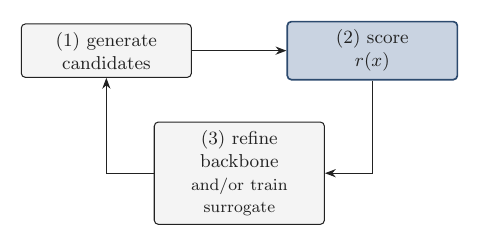
\includegraphics[width=0.55\textwidth]{figures/diagram_active_loop.png}
  \caption{\textbf{Active loop.} The high-level structure shared by every fine-tuning method we evaluate: generate candidates, score them under the oracle, then refine the backbone $p_\theta$ and/or the surrogate before generating again.}
  \label{fig:diag_active}
\end{figure}

{\begin{algorithm}[H]
\caption{Online active loop with the five composable knobs (finetuner-agnostic). Schematic in Fig.~\ref{fig:test_time_feedback}.}
\label{alg:method}
\begin{algorithmic}[1]
\Require Pretrained $p_{\text{pre}}$, oracle $r(\cdot)$, fine-tuning loss $\mathcal{L}_{\text{ft}}$, wall budget $T_{\text{wall}}$
\Require Generation batch $M$, oracle batch $K$, fine-tuning steps per round $G$
\Require Reward-shape: CVaR quantile $q$, debiasing $\gamma$, invalid penalty $r_{\text{inv}}$; ensemble size $J$
\State Initialize $p_{\theta_0} \leftarrow p_{\text{pre}}$;~ buffer $\mathcal{B} \leftarrow \emptyset$;~ ensemble $\{\hat{r}_{\phi_j}\}_{j=1}^{J}$ random
\While{wall time $< T_{\text{wall}}$}
    \State $C_t \leftarrow$ sample $M$ candidates from $p_{\theta_t}$
    \State $(\mu_i, \sigma_i) \leftarrow$ ensemble mean/std on $x_i \in C_t$
    \State $\hat r_i \sim \mathcal{N}(\mu_i, \sigma_i^2)$ \Comment{\emph{(4) Thompson sampling}}
    \State $S_t \leftarrow$ top-$K$ of $C_t$ by $\hat r_i$
    \For{$x \in S_t$}
        \State $r_x \leftarrow r_{\text{inv}}$ if $x$ fails RDKit parse \textbf{else} $r(x)$ \Comment{\emph{(3) invalid-SMILES penalty}}
        \State $\mathcal{B} \leftarrow \mathcal{B} \cup \{(x, r_x)\}$ \Comment{\emph{(5) replay buffer}}
    \EndFor
    \State $\tau \leftarrow Q_q(\{r : (\cdot, r) \in \mathcal{B}\})$
    \For{$g = 1, \ldots, G$}
        \State sample mini-batch $\mathcal{B}_b \subset \mathcal{B}$
        \State $r^*(x) \leftarrow (r_x - \tau)_+ / (1-q)$ \Comment{\emph{(1) CVaR shaping}}
        \State $\log \tilde{r}(x) \leftarrow \log r^*(x) - \gamma \log p_{\theta_t}(x)$ \Comment{\emph{(2) model debiasing}}
        \State update $p_{\theta_t}$ via $\mathcal{L}_{\text{ft}}$ on $\mathcal{B}_b$ using $\log \tilde{r}$ as the per-sample reward
    \EndFor
    \State refit ensemble $\{\hat{r}_{\phi_j}\}$ on $\mathcal{B}$
\EndWhile
\State \Return $\arg\max_{x \in \mathcal{B}} r_x$
\end{algorithmic}
\end{algorithm}}

\subsection{Fine-tuning objective and exploration knobs}

\begin{figure}[H]
  \centering
  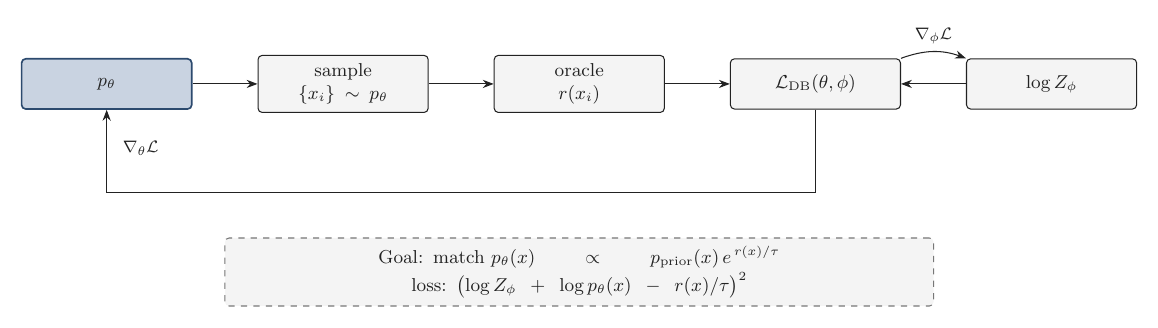
\includegraphics[width=0.95\textwidth]{figures/diagram_ddpp.png}
  \caption{\textbf{DDPP-LB loss.} Trajectory-balance squared residual matching $q_\theta$ to the reward-tilted posterior $p^\star \propto p_{\text{pre}} \cdot r$, with a learned partition-function head $\hat{Z}_\phi$ trained jointly with $\theta$.}
  \label{fig:diag_ddpp}
\end{figure}

\begin{figure}[H]
\centering
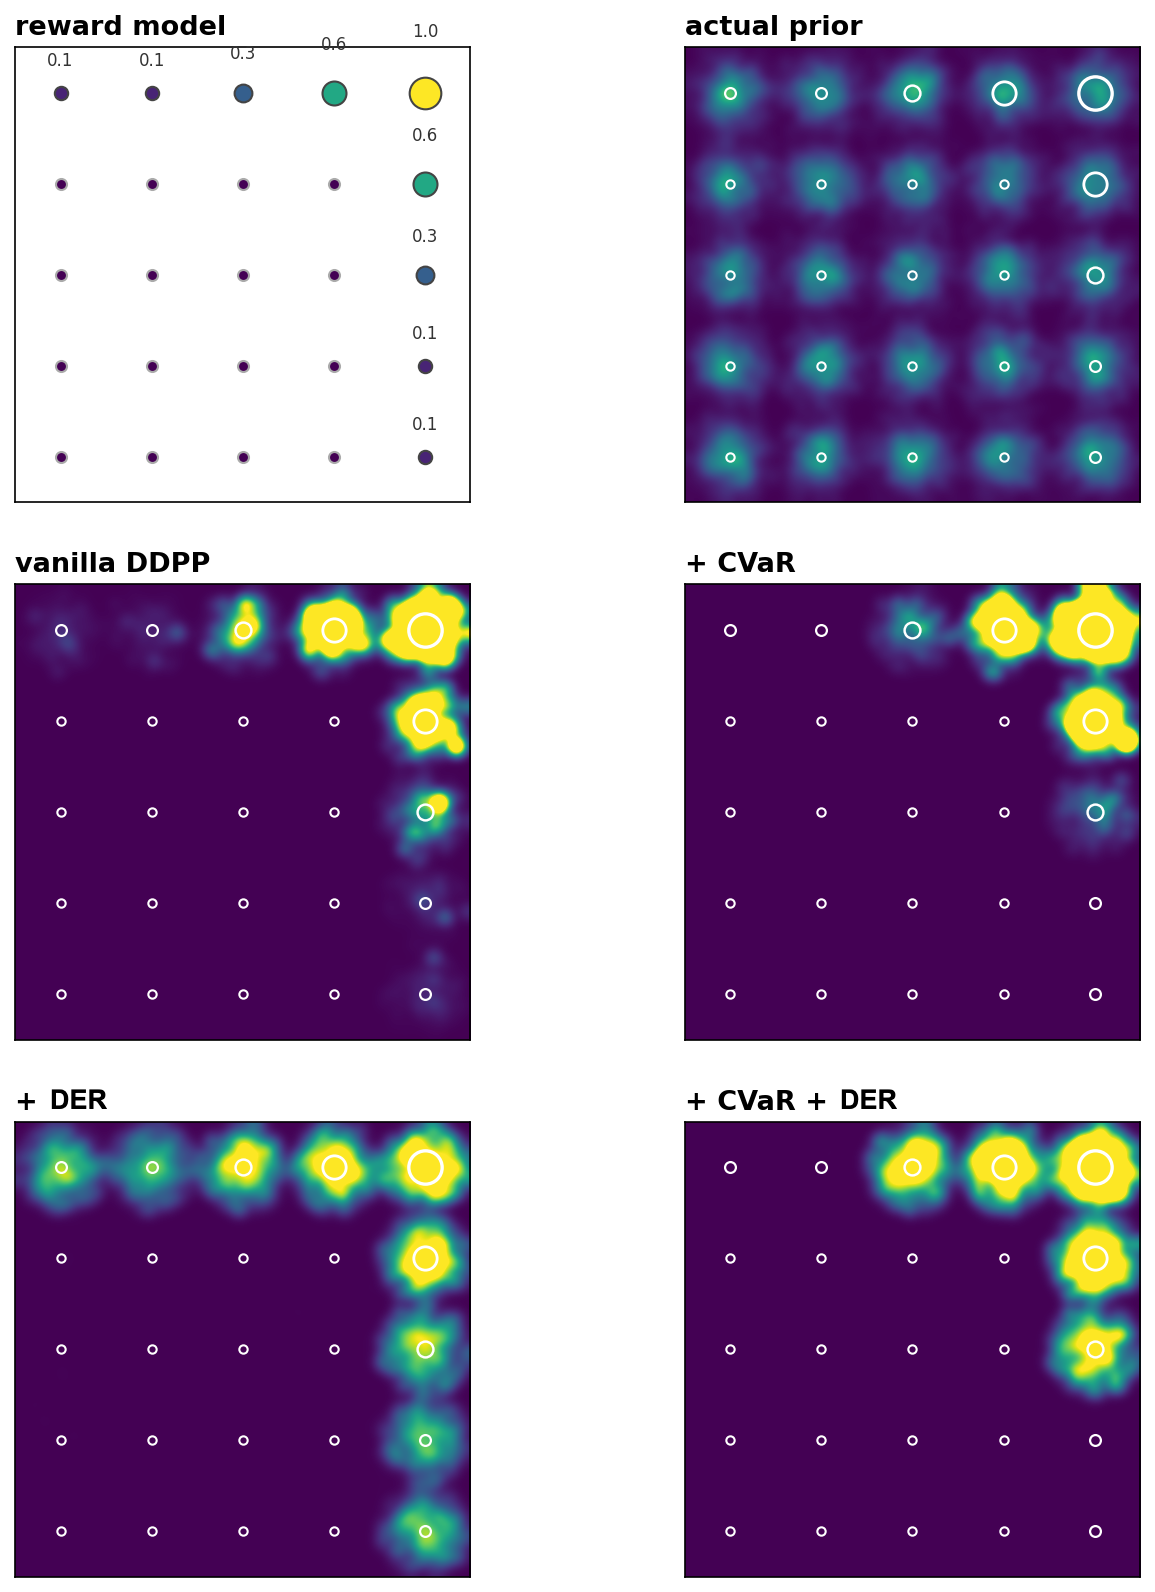
\includegraphics[width=0.85\textwidth]{figures/synthetic_distribution_evolution.png}
\caption{\textbf{Reward shapes on a synthetic 25-mode landscape.} (a) Prior $p_{\text{anchor}}$: 25 roughly Gaussian modes. (b) Each mode is assigned a score in $[0,1]$. (c) Vanilla DDPP-LB with raw reward $r(x)$ puts mass on modes proportional to their reward weight (ideal under unlimited sampling, but compute-inefficient under limited oracle calls). (d) CVaR shaping concentrates most mass on the $r \geq 0.3$ modes, enabling deeper search of the top-reward modes. (e) Model debiasing $\log \tilde r(x)=\log \tilde r_{\mathrm{cvar}}(x) - \gamma \log p_{\theta_t}(x)$ flattens probability mass across rewarded modes, allowing rare high-scoring molecules in less-likely modes to be discovered. (f) CVaR $+$ model debiasing yields a roughly uniform distribution over the top-$\tau$ modes, preventing CVaR's early collapse while preserving its tail focus.}
\label{fig:synth_dist_evolution}
\end{figure}

\begin{figure}[H]
  \centering
  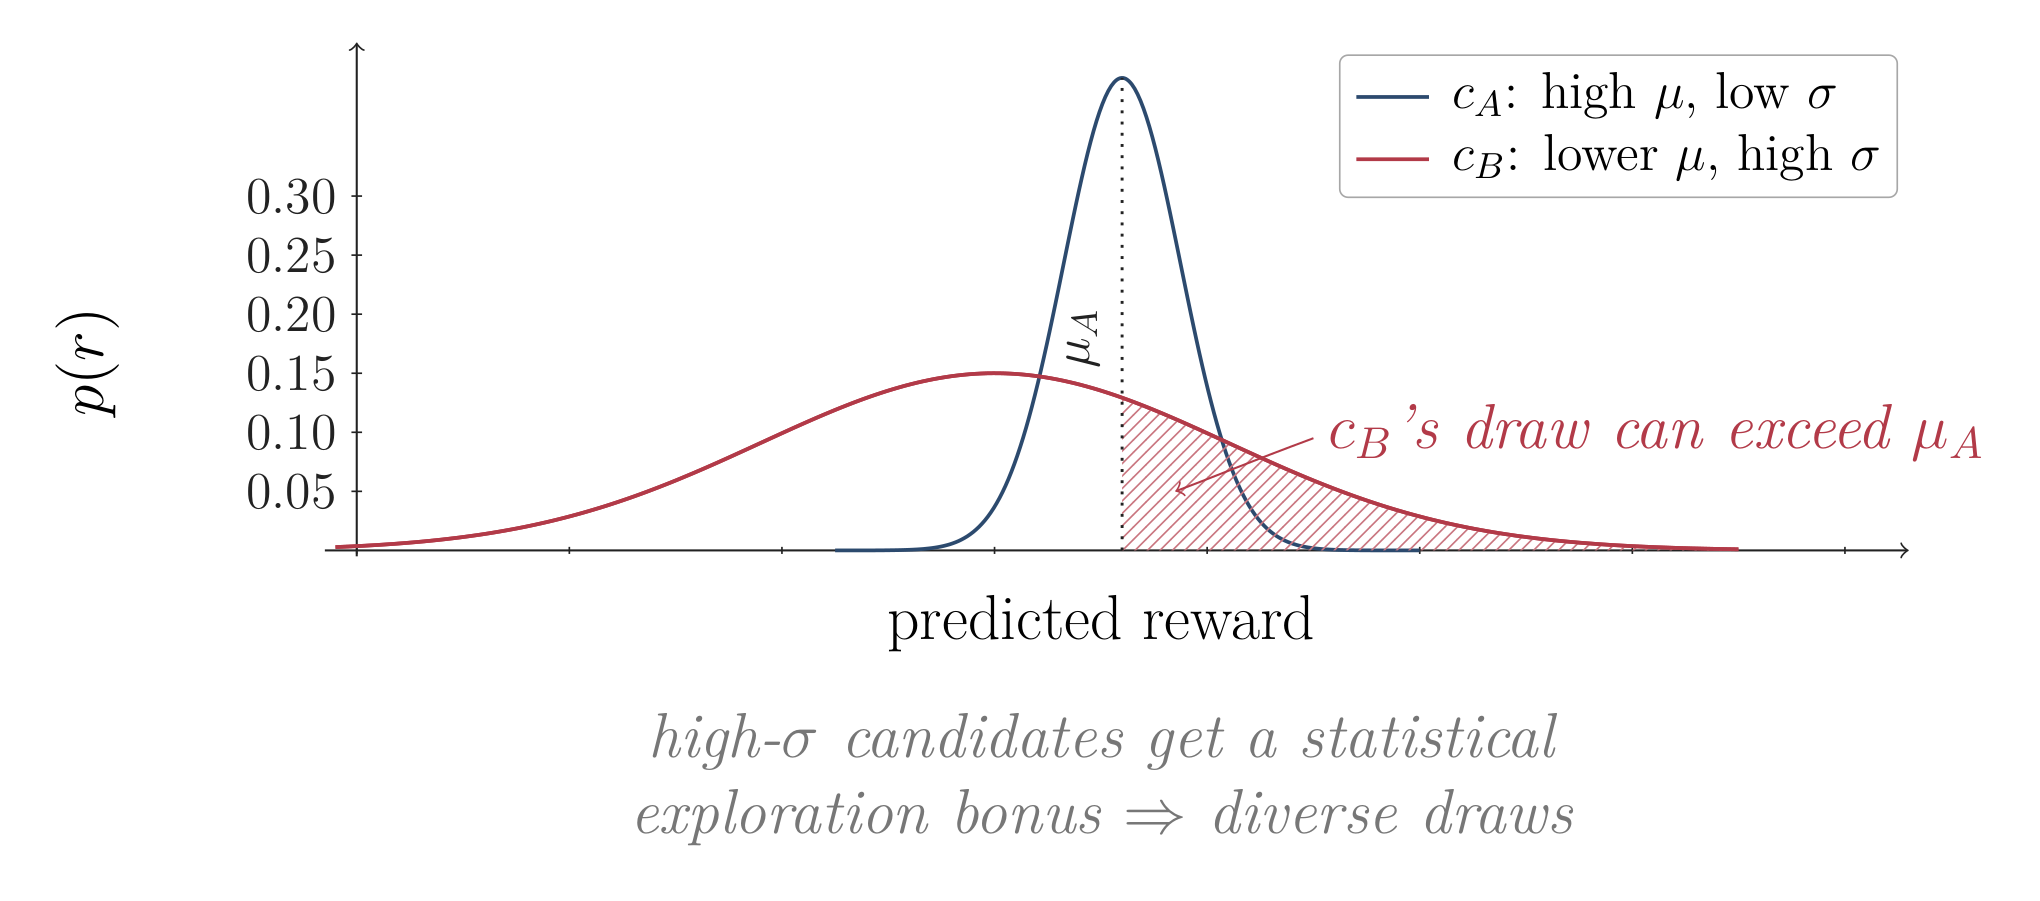
\includegraphics[width=0.65\textwidth]{figures/diagram_thompson.png}
  \caption{\textbf{Thompson sampling.} Acquisition rule: a per-candidate sampled surrogate reward $\hat r_i = \mu_i + \varepsilon_i \sigma_i$ over the ensemble's mean/disagreement, oracle-evaluating the top-$K$ by $\hat r_i$. Different draws of $\varepsilon$ favor different molecular regions.}
  \label{fig:diag_thompson}
\end{figure}

\begin{figure}[H]
  \centering
  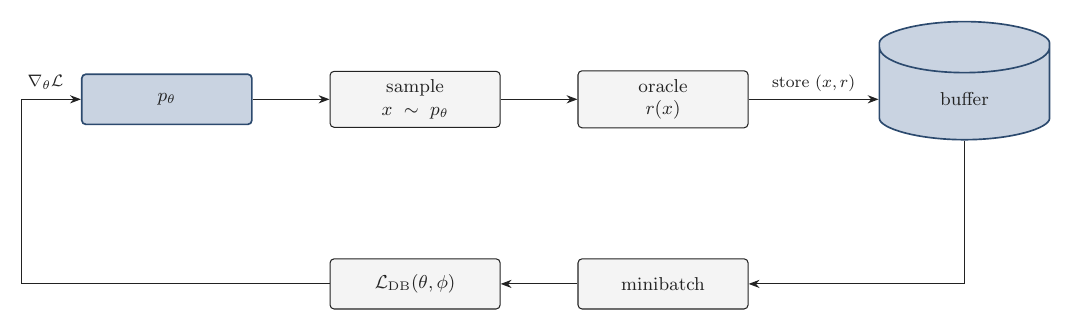
\includegraphics[width=0.95\textwidth]{figures/diagram_buffer.png}
  \caption{\textbf{Replay buffer.} Each generated $(x, r)$ pair is stored in a fixed-capacity buffer with priority eviction; mini-batches are drawn from the buffer (with a fixed fresh-fraction) so the gradient sees a time-averaged version of the policy distribution rather than the sharp on-policy one.}
  \label{fig:diag_buffer}
\end{figure}

\subsection{Inference-time search families}

\begin{figure}[H]
  \centering
  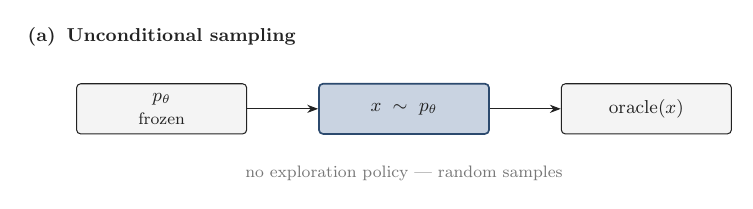
\includegraphics[width=0.55\textwidth]{figures/diagram_uncond.png}
  \caption{\textbf{Unconditional sampling.} The simplest baseline: sample from $p_\theta$ and score every sample under the oracle, with no exploration policy.}
  \label{fig:diag_uncond}
\end{figure}

\begin{figure}[H]
  \centering
  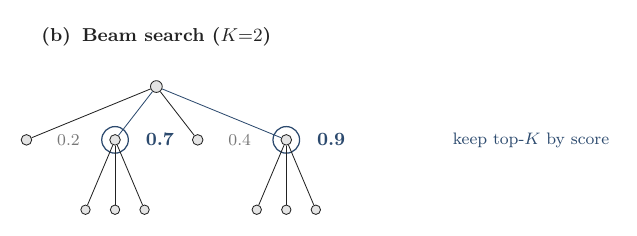
\includegraphics[width=0.7\textwidth]{figures/diagram_beam.png}
  \caption{\textbf{Beam search.} At each denoising step, the top-$K$ partial trajectories by score are kept and expanded; the rest are pruned.}
  \label{fig:diag_beam}
\end{figure}

\begin{figure}[H]
  \centering
  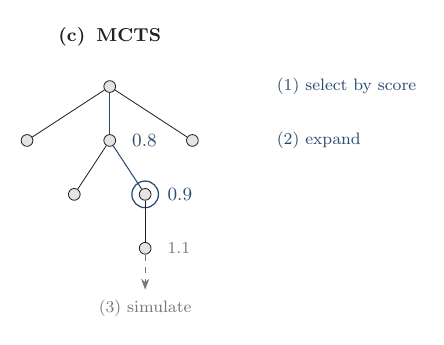
\includegraphics[width=0.7\textwidth]{figures/diagram_mcts.png}
  \caption{\textbf{Monte Carlo Tree Search.} Each node is a partial denoising state; UCB selects the next expansion based on visit counts and value estimates from rollouts.}
  \label{fig:diag_mcts}
\end{figure}

\begin{figure}[H]
  \centering
  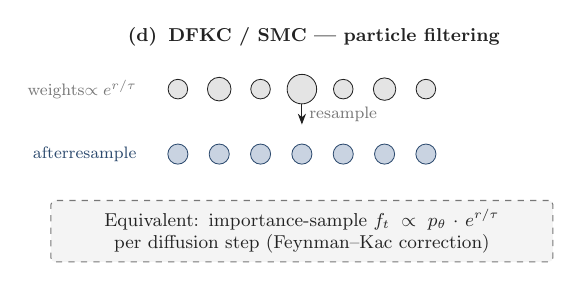
\includegraphics[width=0.7\textwidth]{figures/diagram_dfkc.png}
  \caption{\textbf{Discrete Feynman-Kac correctors (DFKC) / SMC.} A particle population is reweighted at each denoising step by a tilt proportional to the (estimated) reward, then resampled when effective sample size drops below threshold.}
  \label{fig:diag_dfkc}
\end{figure}

\subsection{Surrogate and Tweedie shortcuts}

\begin{figure}[H]
  \centering
  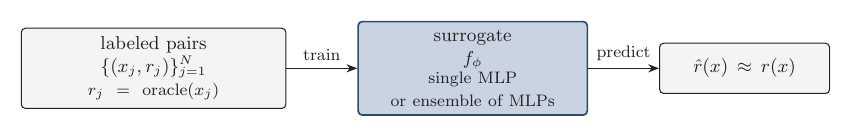
\includegraphics[width=0.7\textwidth]{figures/diagram_surrogate.png}
  \caption{\textbf{Surrogate screening.} A cheap learned surrogate $\hat{r}(x_t)$ scores intermediate states in place of the expensive oracle, reducing per-output oracle cost from $O(L)$ to $O(1)$.}
  \label{fig:diag_surrogate}
\end{figure}

\begin{figure}[H]
  \centering
  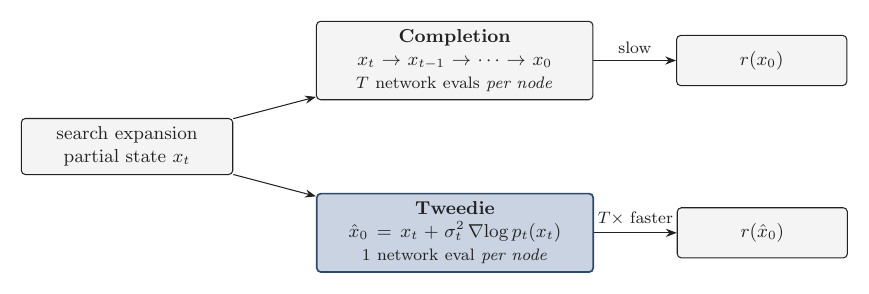
\includegraphics[width=0.7\textwidth]{figures/diagram_tweedie.png}
  \caption{\textbf{Tweedie estimator.} The posterior-mean denoised state $\hat{x}_0 = \mathbb{E}[x_0 \mid x_t]$ is computed in a single denoising pass and scored directly, replacing a full rollout \citep{efron2011tweedie, chung2023dps}.}
  \label{fig:diag_tweedie}
\end{figure}

\clearpage

\section{Component Ablations and Diagnostics}\label{app:component-analysis}

This section moves from controlled single-component comparisons to diagnostics, joint effects, and transfer across fine-tuning objectives.

% Previous heading: \subsection{Knob interactions: acquisition vs.\ reward shaping}\label{app:knob-interactions}
\subsection{Roles of Acquisition and Reward Shaping}\label{app:knob-interactions}

This subsection collects the longer descriptions of how Thompson-sampling acquisition and model-debiasing reward shaping individually act on the loop, moved here from Sec.~\ref{sec:design-explore} for brevity.

\paragraph{Thompson sampling vs.\ deterministic top-$\mu$ selection.} The contrast with deterministic top-$\mu$ selection is sharp (Fig.~\ref{fig:diag_thompson_body}): under deterministic selection a candidate $c_B$ with $\mu_B < \mu_A$ never gets oracle-evaluated, no matter how uncertain it is, so the training data $(x, r(x))$ that downstream finetuning sees is concentrated on the current surrogate argmax. As the ensemble disagreement $\sigma_B$ grows away from zero, the Thompson rule smoothly transitions from this hard-greedy regime to a stochastic exploration bonus, the standard way to guard against local optima \citep{chapelle2011empirical}. The acquisition step is itself modifying which samples from $p_{\theta_t}$ enter the evaluated set and therefore which data the gradient computes against. Fig.~\ref{fig:thompson_acquisition} measures this directly: against a reward bar set by unconditional sampling rather than by either method, Thompson acquisition clears the bar with $4.5$--$7\times$ more distinct molecules, and the threshold-free view shows why --- greedy selection spends roughly $40\%$ of its oracle budget re-evaluating molecules it has already scored.

\paragraph{Model debiasing as training-dynamics shaping.} At the outer-loop level, $x$ names the candidate being trained on; inside the diffusion objective, this term may be evaluated on the noised or partially denoised state used by the loss. Model debiasing therefore acts on the diffusion training dynamics rather than introducing a separate density estimator over completed molecules. This term favors candidates that are high reward but not already high likelihood under the current generator. It therefore complements Thompson sampling rather than replacing it: Thompson sampling explores uncertainty in the reward surrogate before oracle evaluation, while model debiasing reshapes the training signal after oracle evaluation to avoid repeatedly reinforcing the generator's current modes. Fig.~\ref{fig:diag_debiasing_body} illustrates the redistribution: under the unshaped reward the dominant prior mode keeps absorbing gradient mass; with debiasing the smaller modes get lifted above their prior heights.


% Previous heading: \section{Per-knob individual controlled experiments}\label{app:knobs}
\subsection{Individual Component Ablations}\label{app:knobs}

Each figure isolates one design-choice knob from group~(iii) of Table~\ref{tab:methods}, holding the other knobs at their reference defaults (Table~\ref{tab:hparams}). Every figure is a $3 \times 2$ grid: rows are top-1 best-so-far, top-10 mean, and top-10\% mean; columns are cumulative oracle calls (left) and GPU hours (right).

\paragraph{Reading the top-10\% row.} For inference-time search comparisons (Appendix~\ref{app:search}, e.g.\ Figs.~\ref{fig:surrogate_search} and~\ref{fig:tweedie_search}) the underlying generative distribution is fixed and only the selection procedure changes. Top-10\% mean in those figures reflects sampling efficiency from a static distribution and saturates as the upper tail of $p_{\text{pre}}$ is exhausted. In the active ablations below the policy $q_\theta$ is itself updated, so a continued rise in top-10\% mean is direct evidence that the sampling distribution is shifting --- not just that we are picking better samples from the same distribution.

% Previous heading: \subsection{CVaR reward shaping}
\subsubsection{CVaR reward shaping}

\begin{figure}[H]
  \centering
  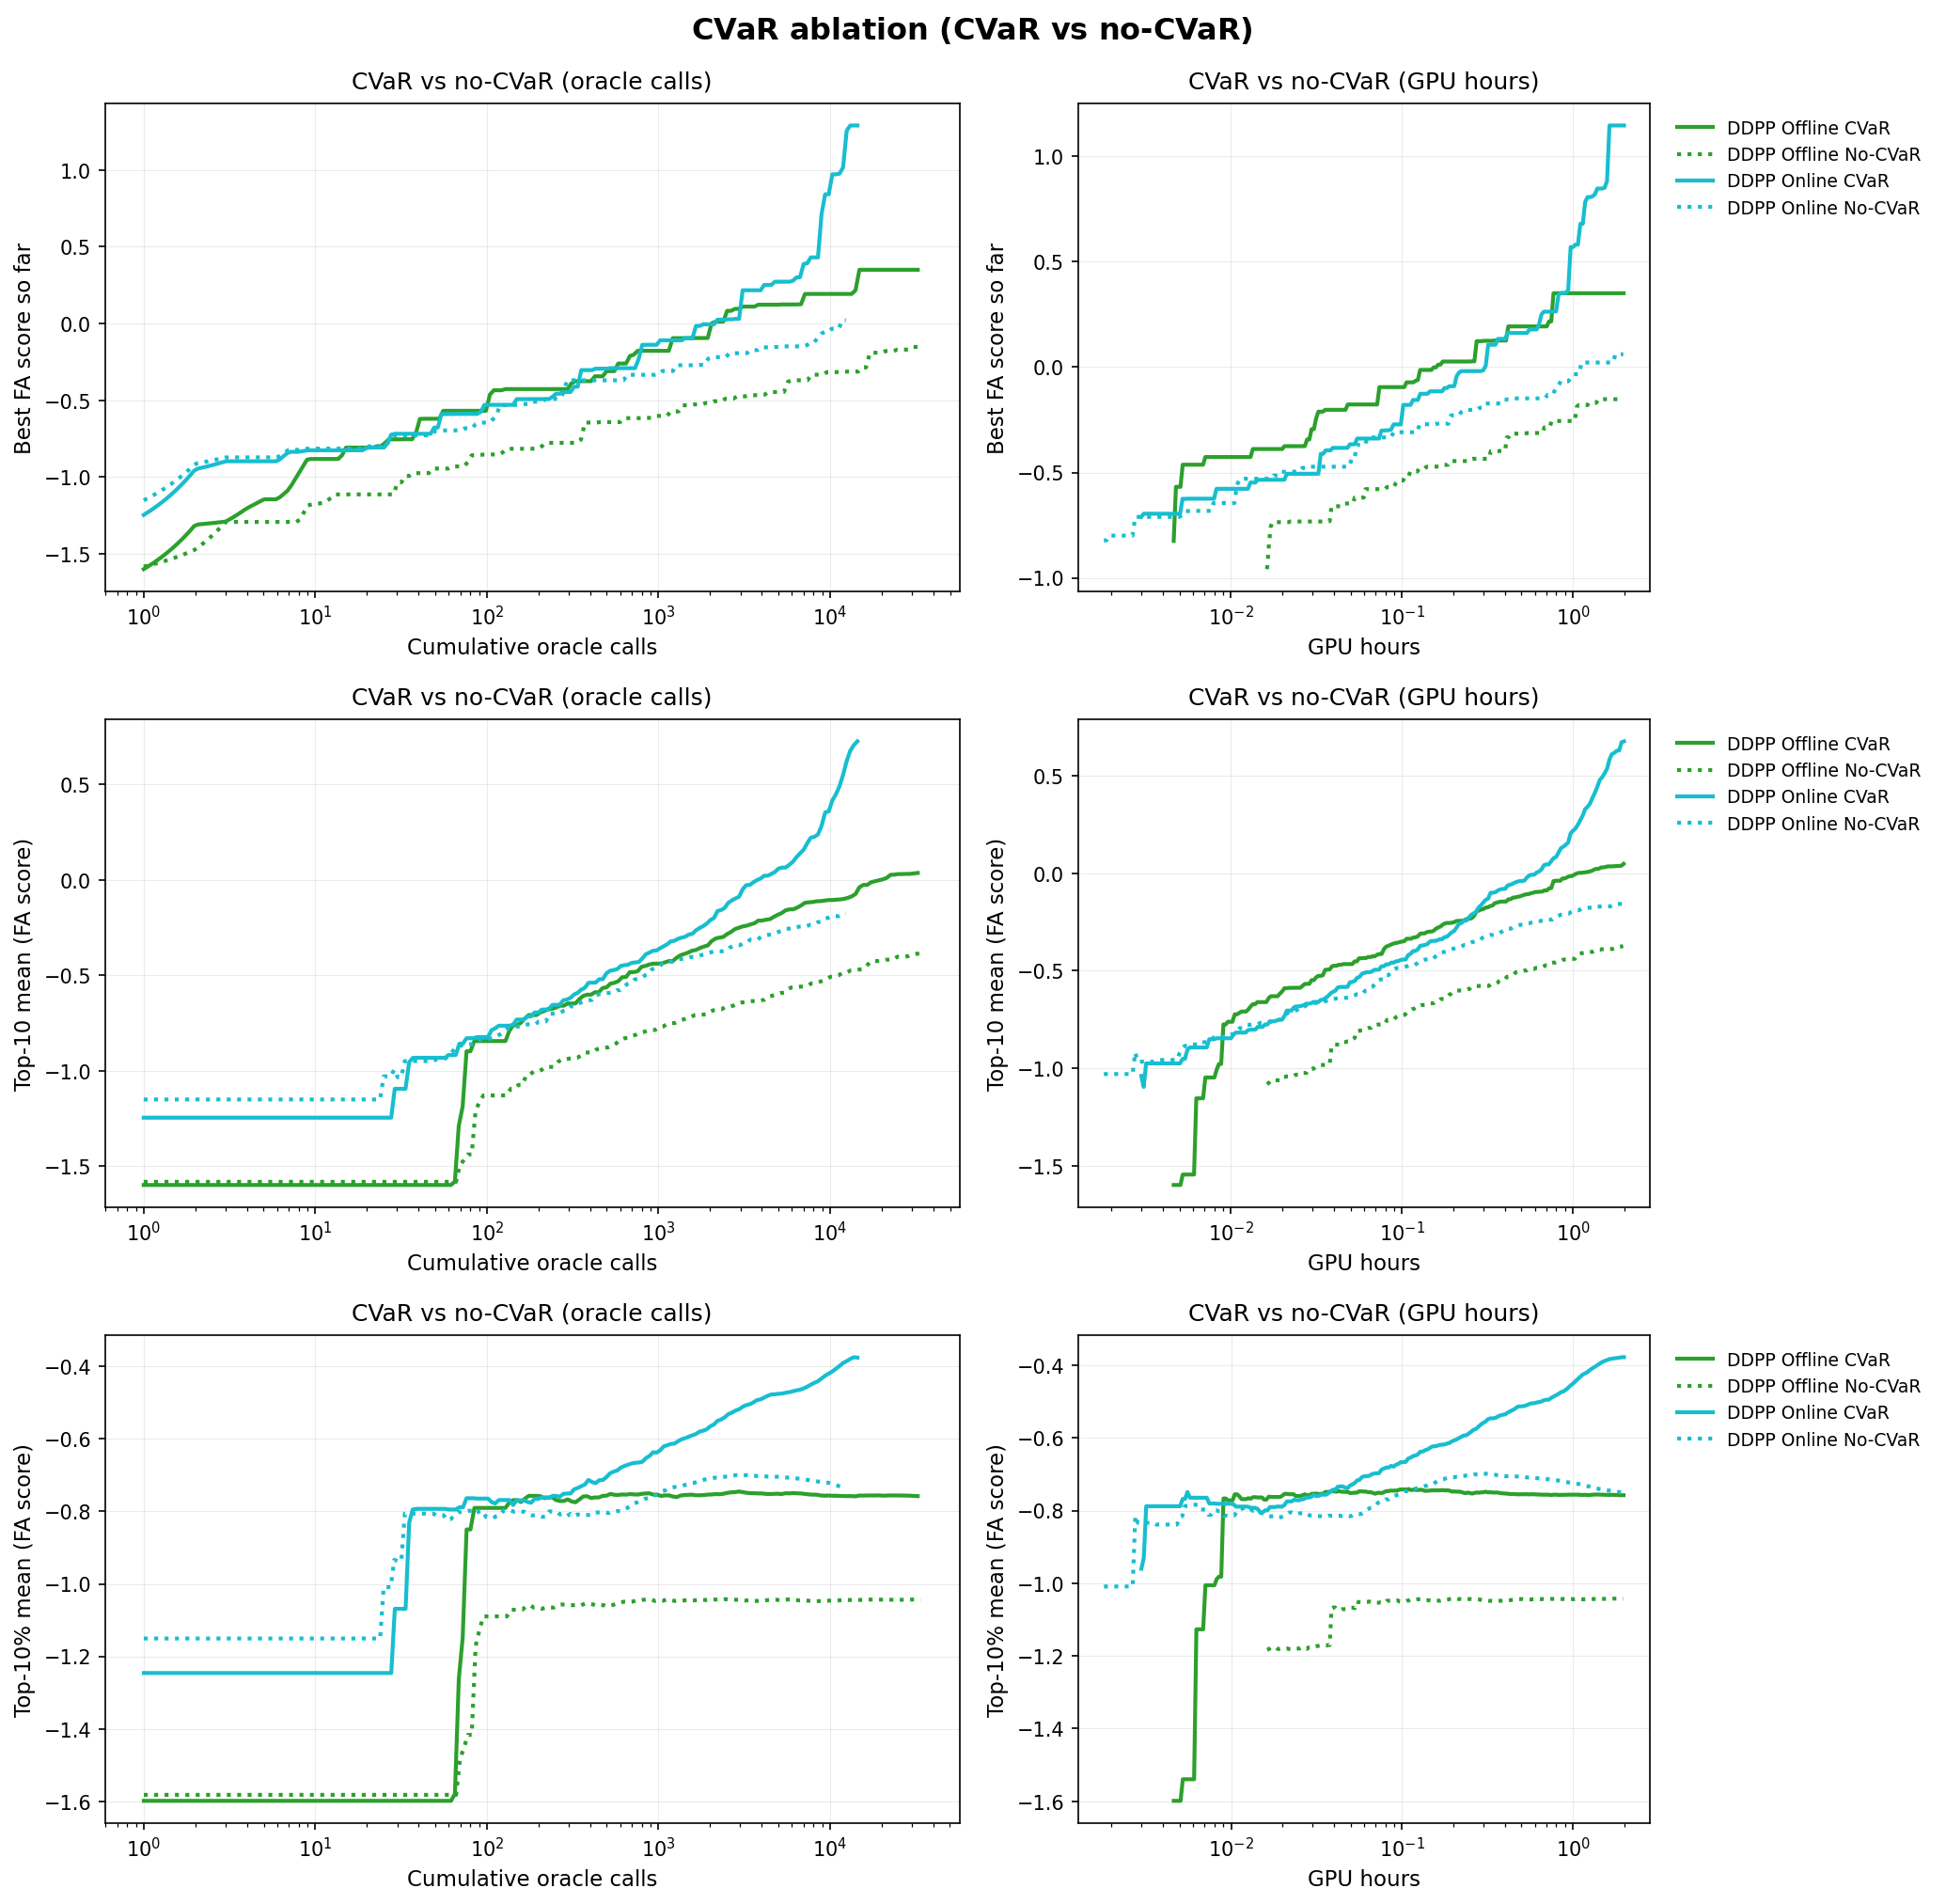
\includegraphics[width=0.95\textwidth]{figures/fig_cvar_3x2.png}
  \caption{\textbf{CVaR ablation.} Four cells on DDPP-LB: solid = CVaR-on, dotted = CVaR-off; green = offline, teal = online. Seed-averaged ($n{=}5$) with $\pm 1$ std bands. CVaR lifts all three metrics in both regimes; the gain on top-10\% mean (bottom row) for the online~$+$~CVaR cell --- which continues to climb to $\sim 0.5$ rather than saturating --- confirms that the CVaR-shaped gradient shifts the policy distribution itself rather than only re-ranking samples from a fixed distribution.}
  \label{fig:cvar_ablation}
\end{figure}

% Previous heading: \subsection{Density Entropy Regularization}
\subsubsection{Density Entropy Regularization}

\begin{figure}[H]
  \centering
  % Previous arXiv-unsafe filename retained for recovery:
% 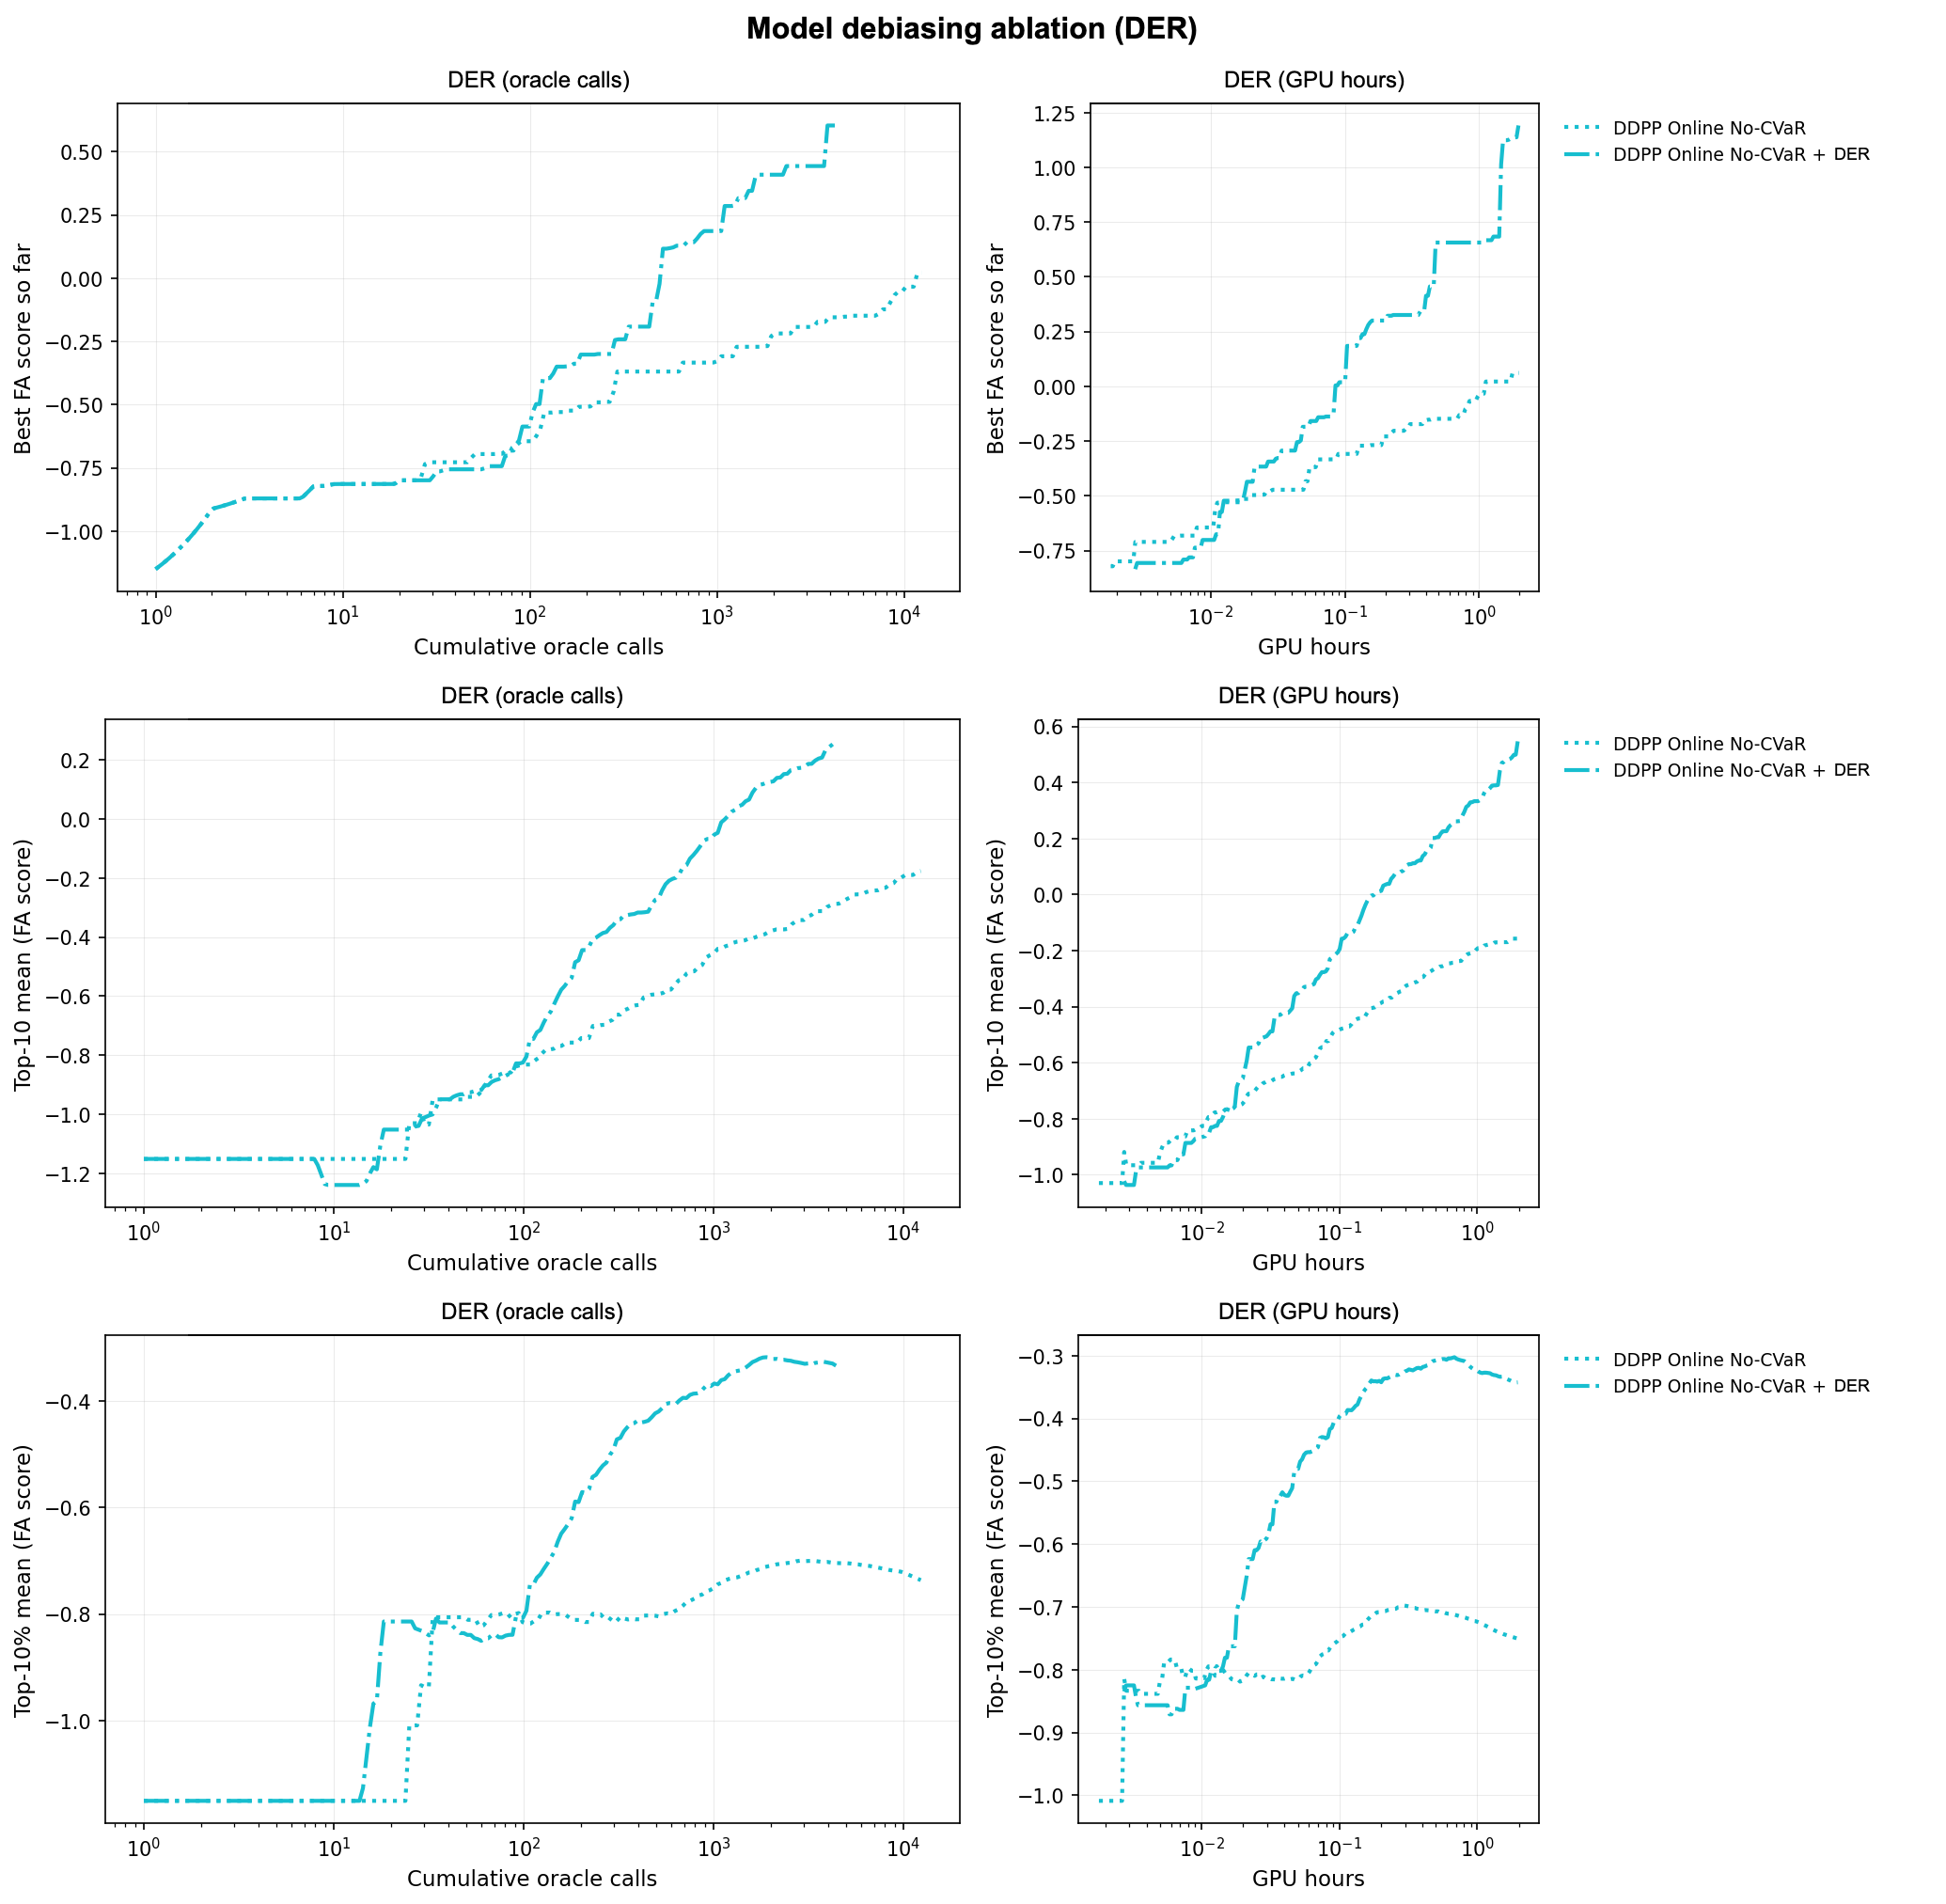
\includegraphics[width=0.95\textwidth]{figures/fig_debiasing_3x2 (1).png}
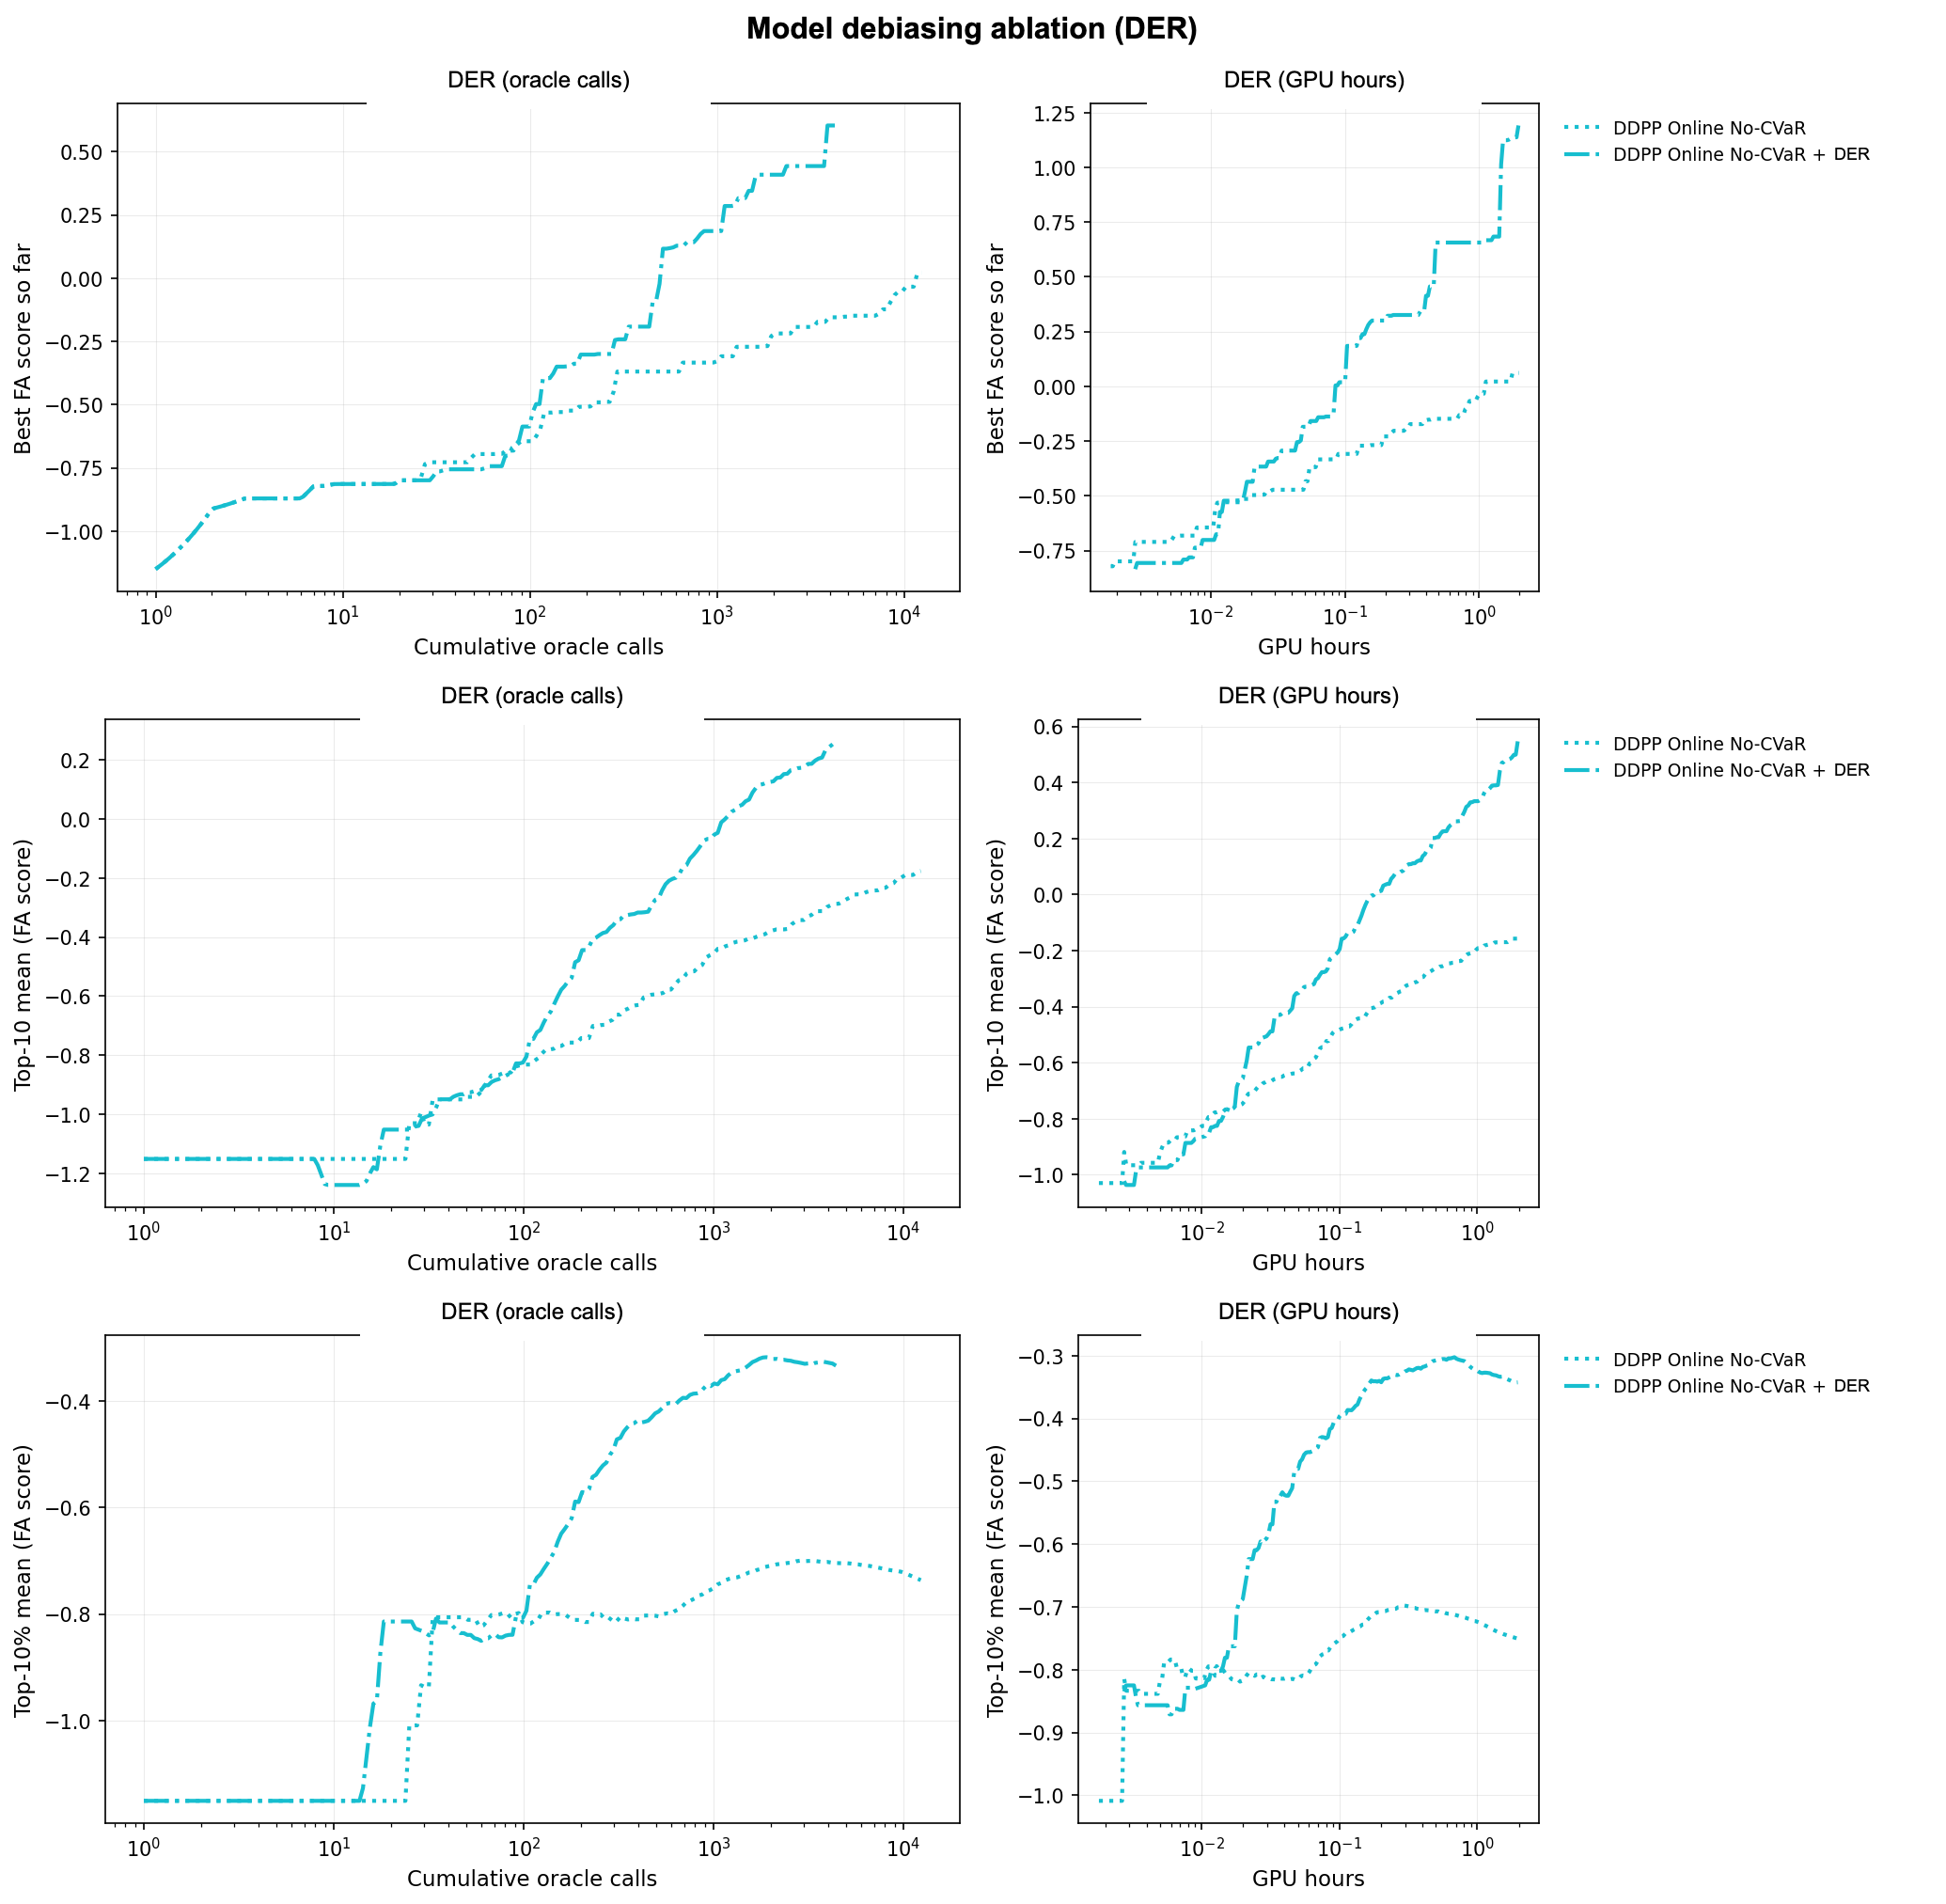
\includegraphics[width=0.95\textwidth]{figures/fig_debiasing_3x2.png}
  \caption{\textbf{Model-debiasing ablation.} Two cells, both online DDPP-LB with CVaR off: solid (with debiasing) vs.\ dotted (without). Seed-averaged ($n{=}5$). Holding CVaR off isolates the debiasing knob from the upper-tail reweighting in Fig.~\ref{fig:cvar_ablation}. Debiasing lifts top-1 by $\sim +0.6$ and top-10\% mean by a comparable margin, again indicating a genuine shift in $q_\theta$ and not just better sample selection.}
  \label{fig:debiasing_ablation}
\end{figure}

% Previous heading: \subsection{Replay buffer}
\subsubsection{Replay buffer}

\begin{figure}[H]
  \centering
  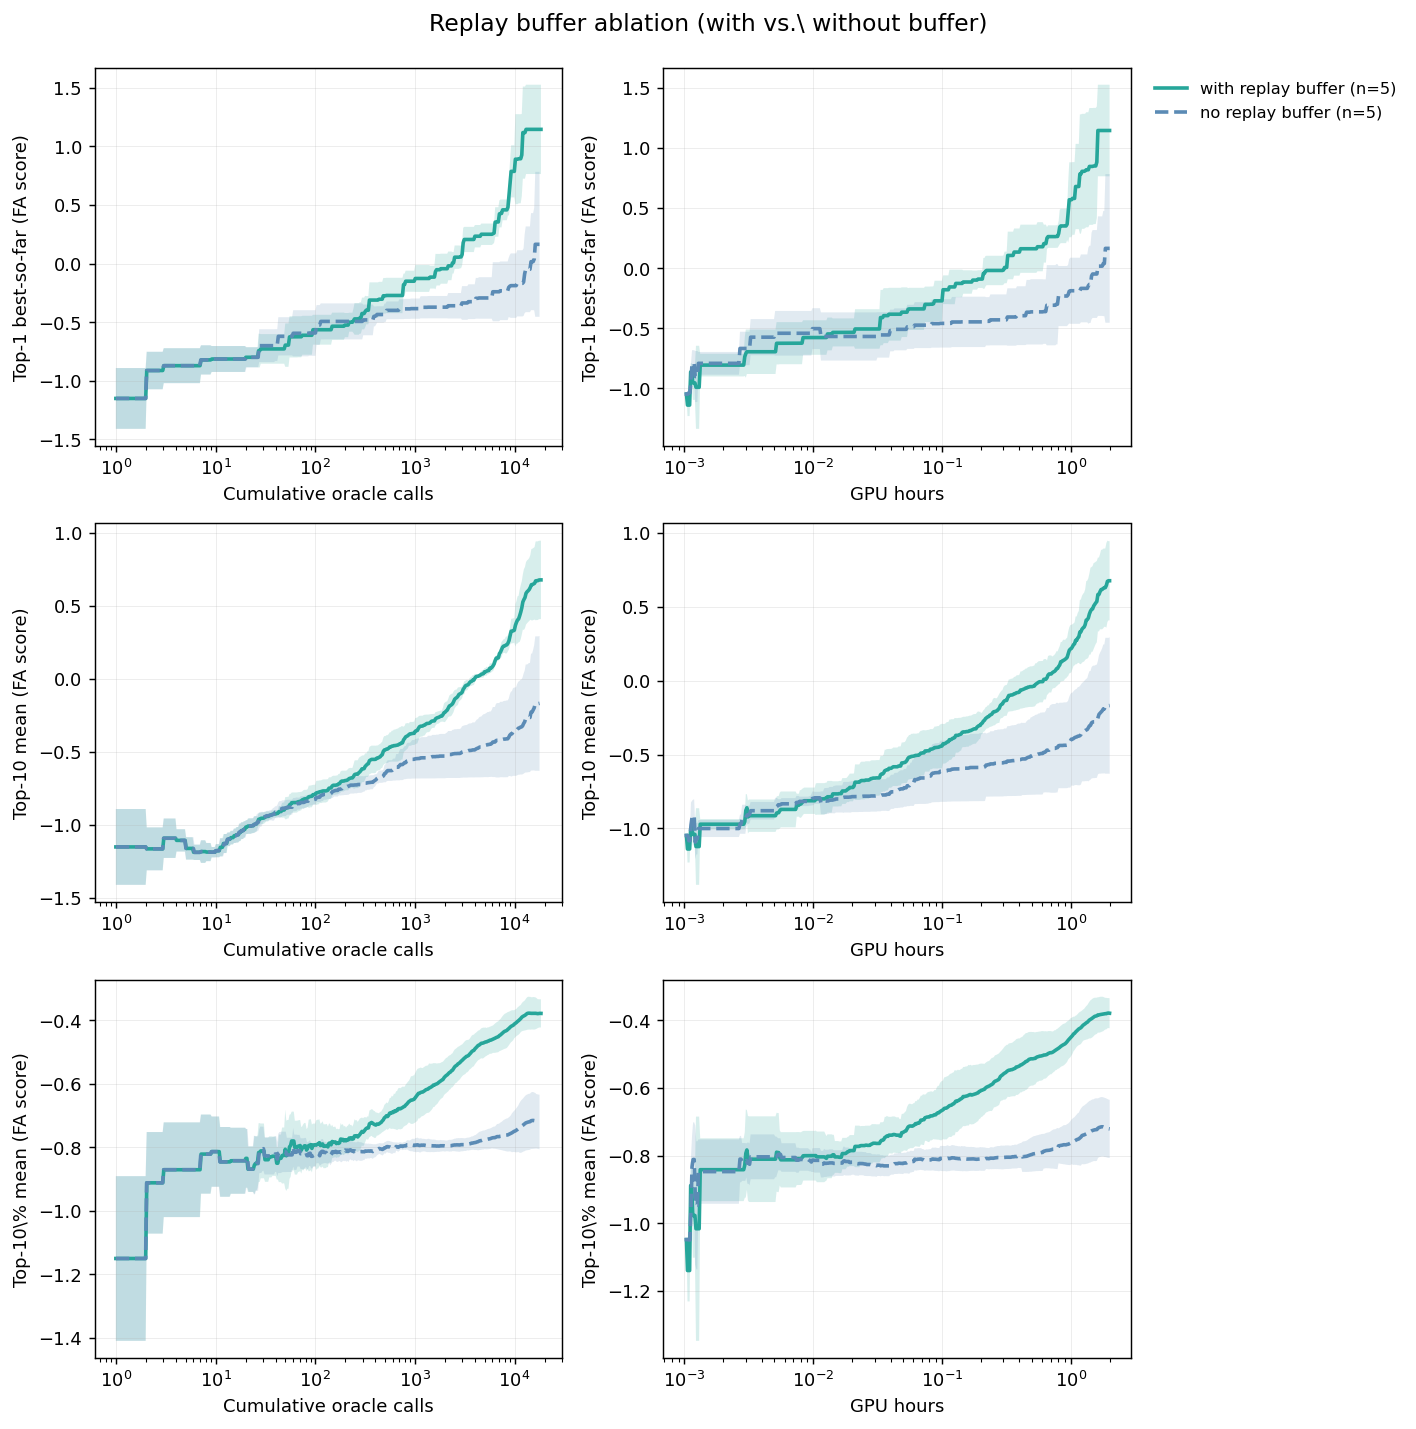
\includegraphics[width=0.95\textwidth]{figures/fig_buffer_2line_3x2.png}
  \caption{\textbf{Replay-buffer ablation.} Two cells, both online DDPP-LB$+$CVaR: solid (with replay buffer) vs.\ dashed (no buffer). Seed-averaged ($n{=}5$). Top-1 separates the cells modestly. The clearest signal is in top-10\% mean (bottom row), where the buffer-on cell continues to climb past $-0.4$ while the buffer-off cell plateaus near $-0.7$. The buffer is shifting where the policy puts mass over the run, not merely re-presenting a fixed set of samples to the gradient.}
  \label{fig:buffer_ablation}
\end{figure}

% Previous heading: \subsection{Thompson acquisition}
\subsubsection{Thompson acquisition}

\begin{figure}[H]
  \centering
  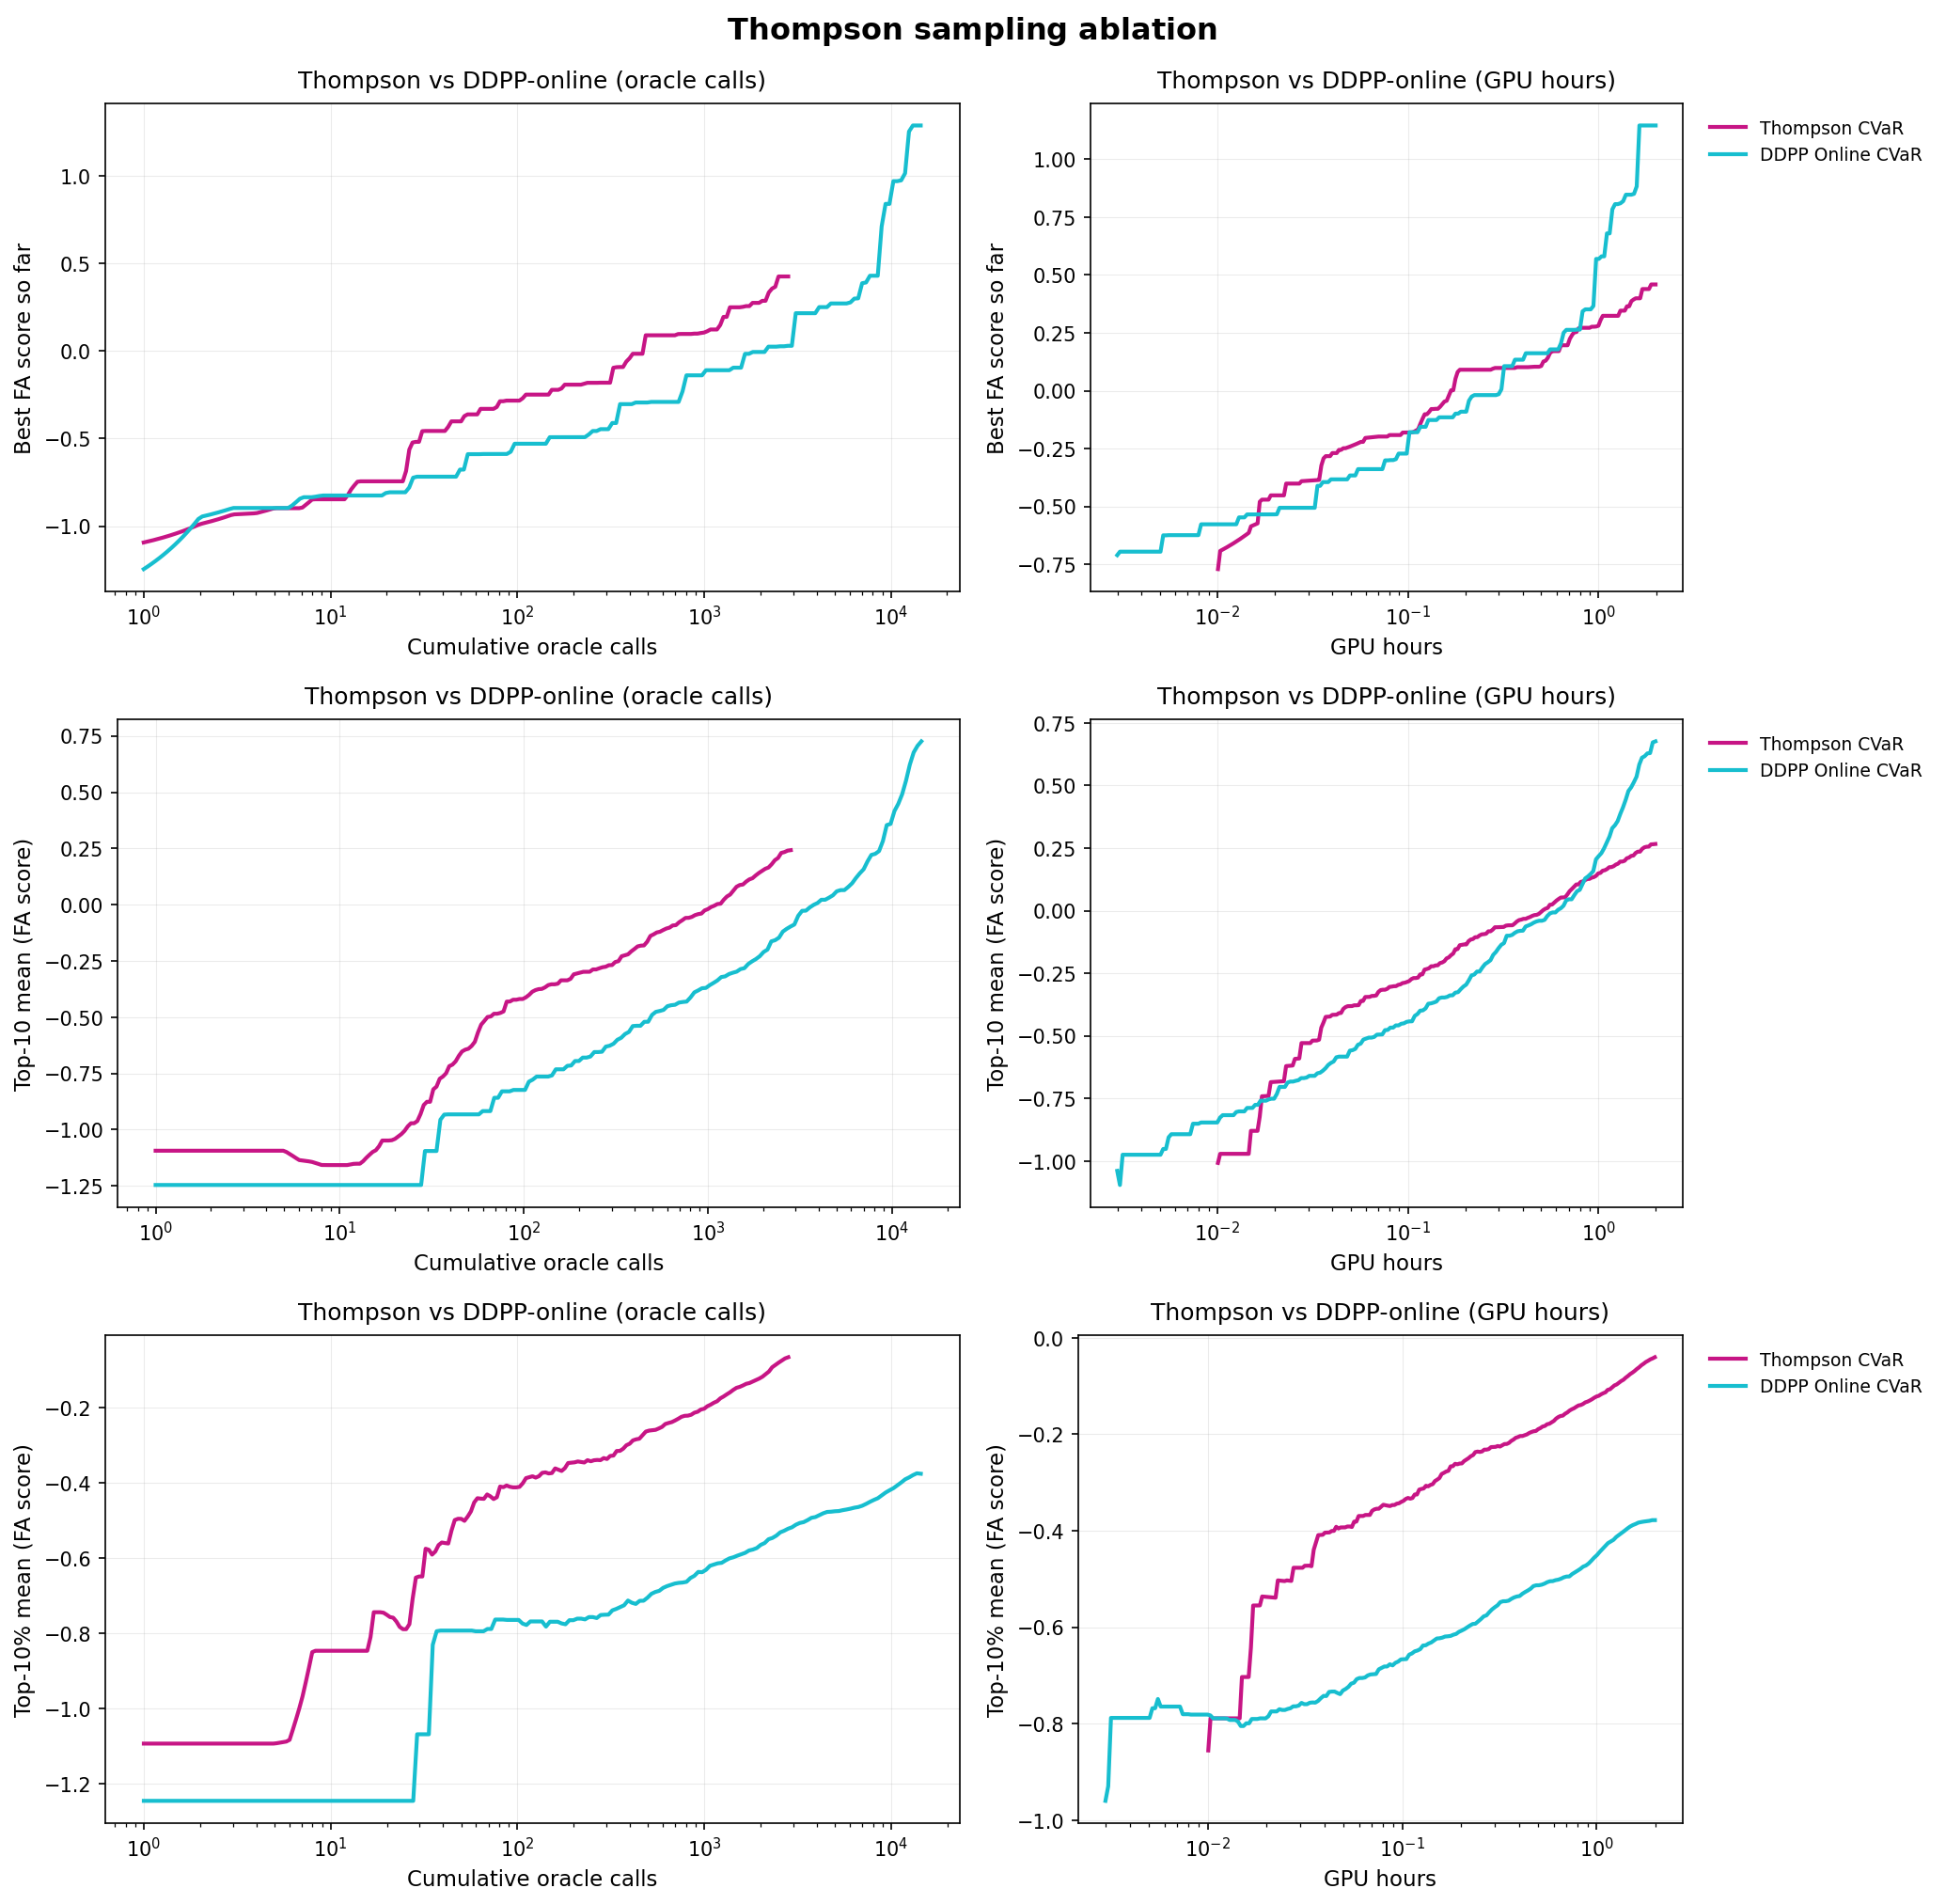
\includegraphics[width=0.95\textwidth]{figures/fig_thompson_3x2.png}
  \caption{\textbf{Thompson-sampling ablation.} Pink: Thompson on top of online DDPP-LB$+$CVaR. Cyan: same configuration with deterministic top-$K$ selection by ensemble mean instead of Thompson draws. Seed-averaged ($n{=}5$). Top-1 is comparable; top-10\% mean (bottom row) is where the contrast is sharpest --- Thompson reaches $\sim -0.05$ vs.\ $\sim -0.4$ for deterministic selection, a clear distribution shift toward higher-reward modes that comes from Thompson diversifying which candidates the oracle is spent on rather than from any change to the gradient itself.}
  \label{fig:thompson_ablation}
\end{figure}

\begin{figure}[H]
  \centering
  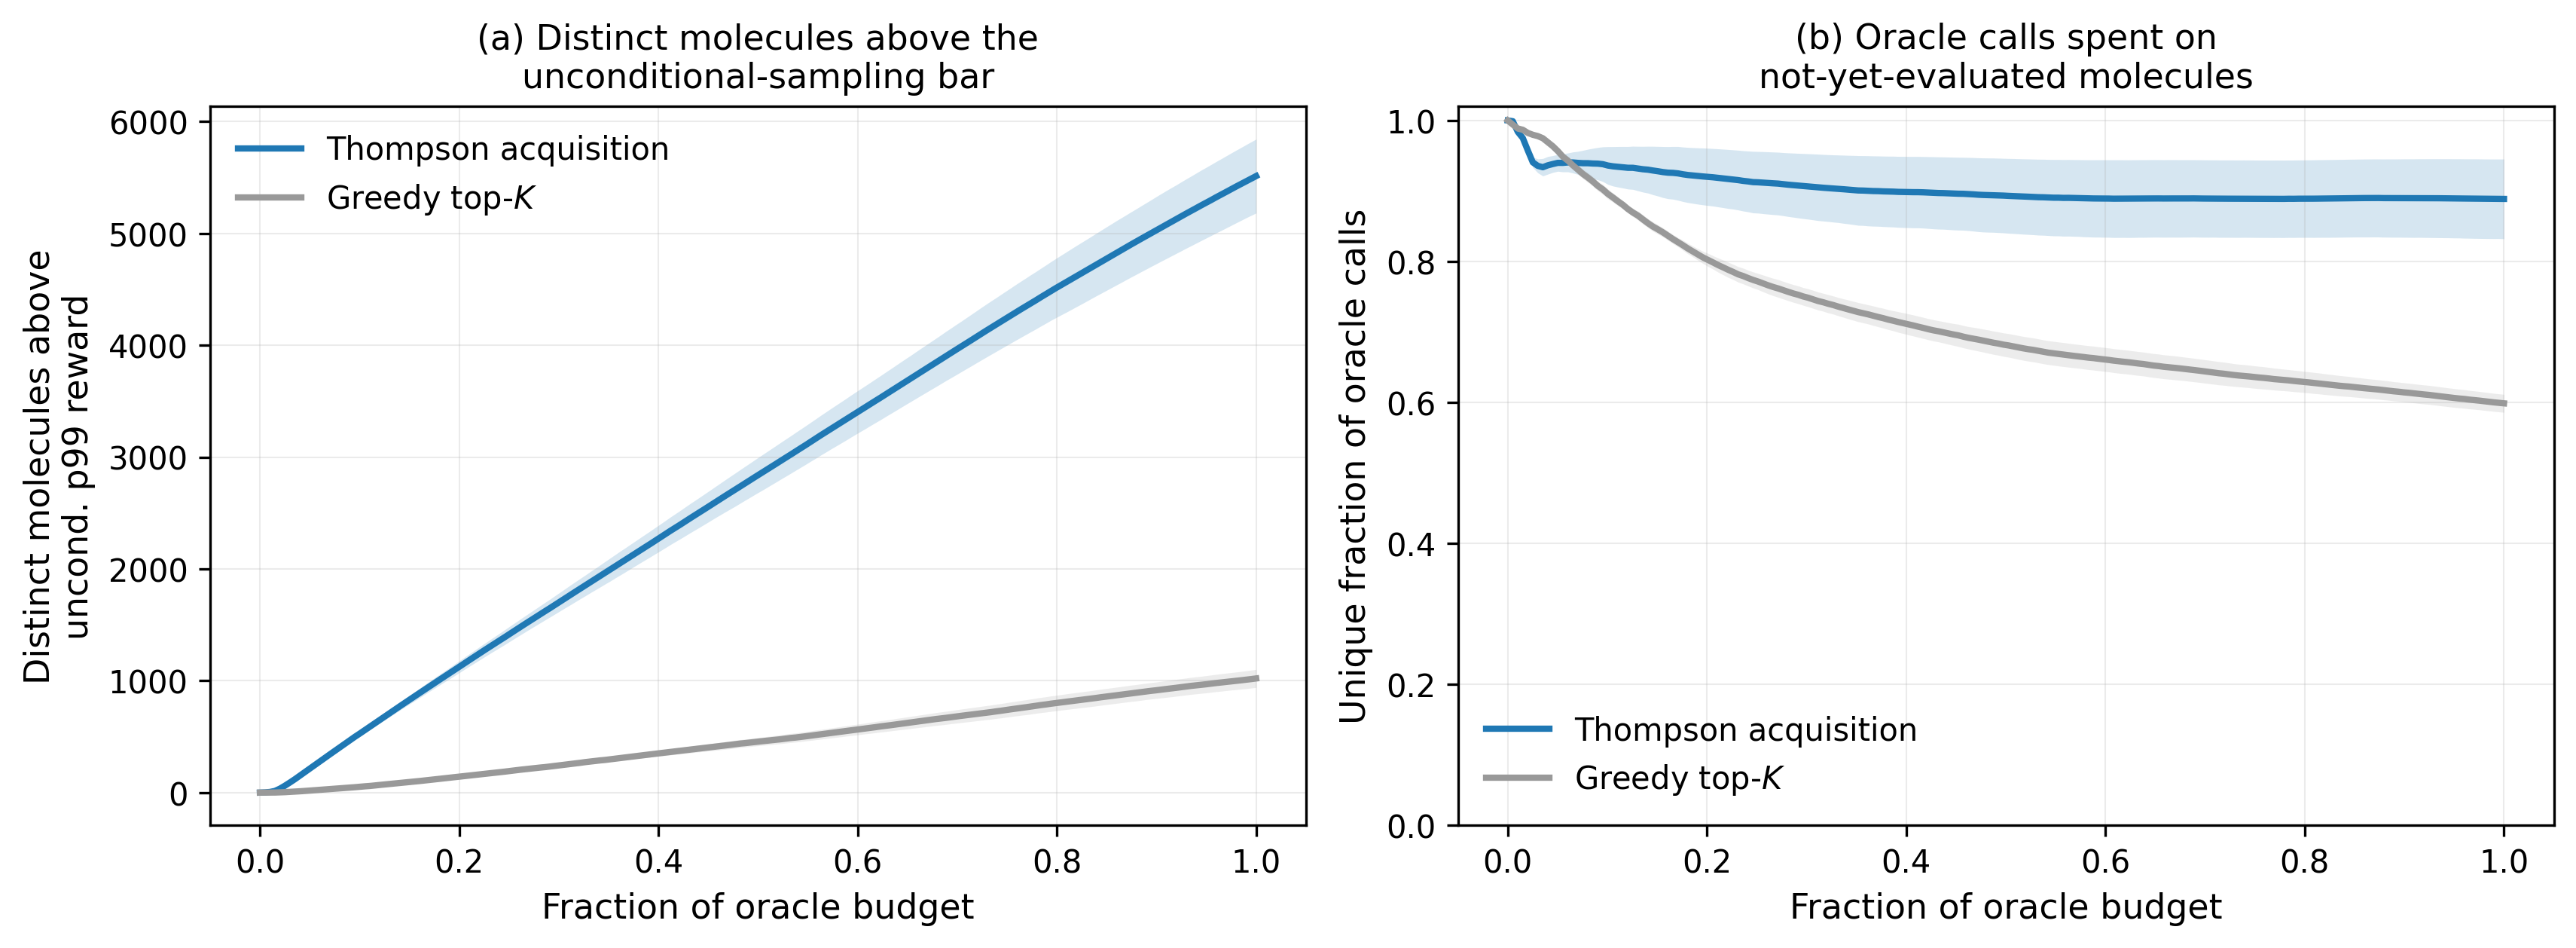
\includegraphics[width=0.95\textwidth]{figures/diagram_thompson_acquisition.png}
  \caption{\textbf{What the uncertainty bonus buys at the acquisition step.} Full DDPP-LB loop (Thompson acquisition) vs.\ the same loop with Thompson disabled, which falls back to greedy top-$K$ by the surrogate's predicted mean; everything else is identical, so the contrast isolates the acquisition rule. Mean over six small-molecule targets $\times$ five seeds, shaded band $\pm 1$ SEM over targets. \textbf{(a)} Distinct molecules found above a per-target bar set by the $99$th percentile of everything the unconditional best-of-$N$ baseline ever evaluated on that target; the bar is external to both methods being compared, so it does not flatter either. Thompson finds $4.5$--$7\times$ more such molecules at the shared final budget. \textbf{(b)} Fraction of oracle calls spent on molecules not already evaluated, which needs no threshold at all. Greedy acquisition keeps re-querying its current favourites and spends roughly $40\%$ of its budget on repeats ($55$--$64\%$ unique, vs.\ $65$--$99.7\%$ for Thompson), which is the mechanism behind the gap in (a).}
  \label{fig:thompson_acquisition}
\end{figure}

% Previous heading: \subsection{Invalid-output penalty}
\subsubsection{Invalid-output penalty}

\begin{figure}[H]
  \centering
  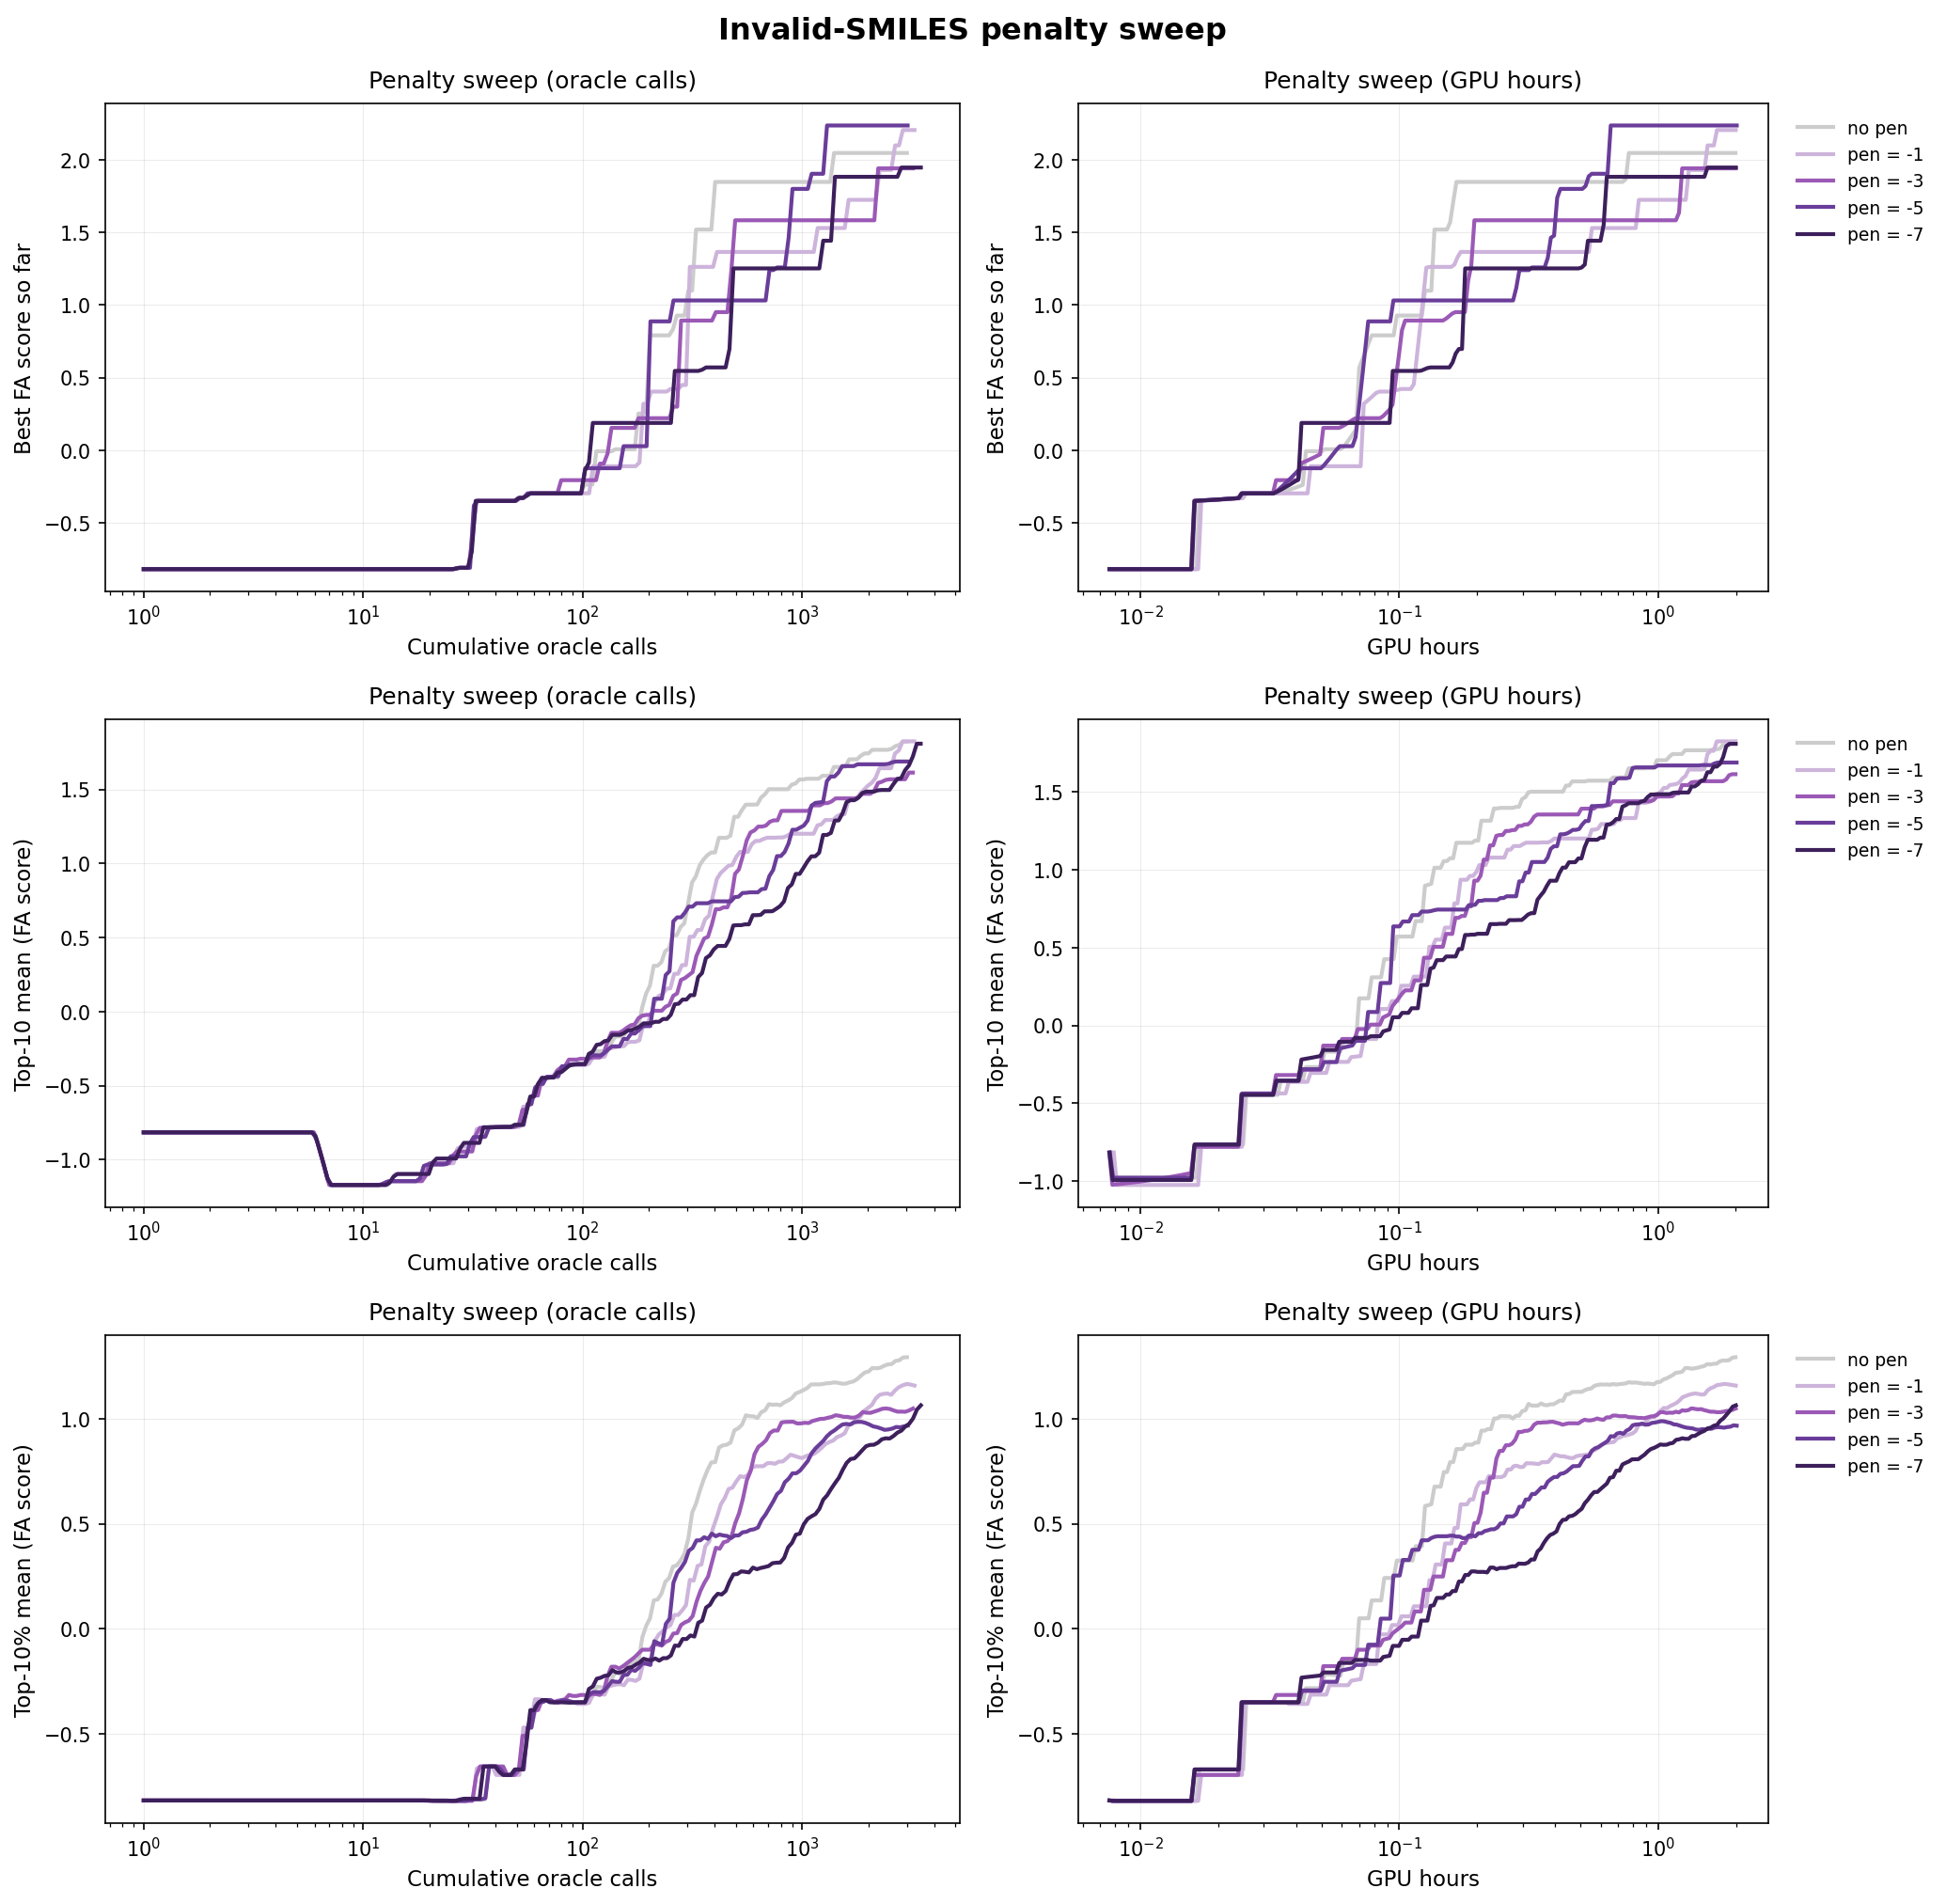
\includegraphics[width=0.95\textwidth]{figures/fig_penalty_3x2.png}
  \caption{\textbf{Invalid-SMILES penalty sweep $r_{\text{inv}} \in \{0, -1, -3, -5, -7\}$.} On top of Approach~A $+$ Thompson. Light-to-dark purple = increasing penalty magnitude. Top-1 and top-10 narrow the gap between cells over time; top-10\% mean separates them most clearly, with smaller penalties ($-1$, $-3$) reaching slightly higher upper-tail FA but at the cost of validity (Fig.~\ref{fig:penalty_sweep}). $r_{\text{inv}} = -5$ achieves the best validity / top-1 FA trade-off across the sweep. Effect is not very signifcant on regular DDPP-LB but becomes much more significant with other exploratory methods, as seen in the ablation figures.}
  \label{fig:penalty_ablation}
\end{figure}

\begin{figure}[H]
  \centering
    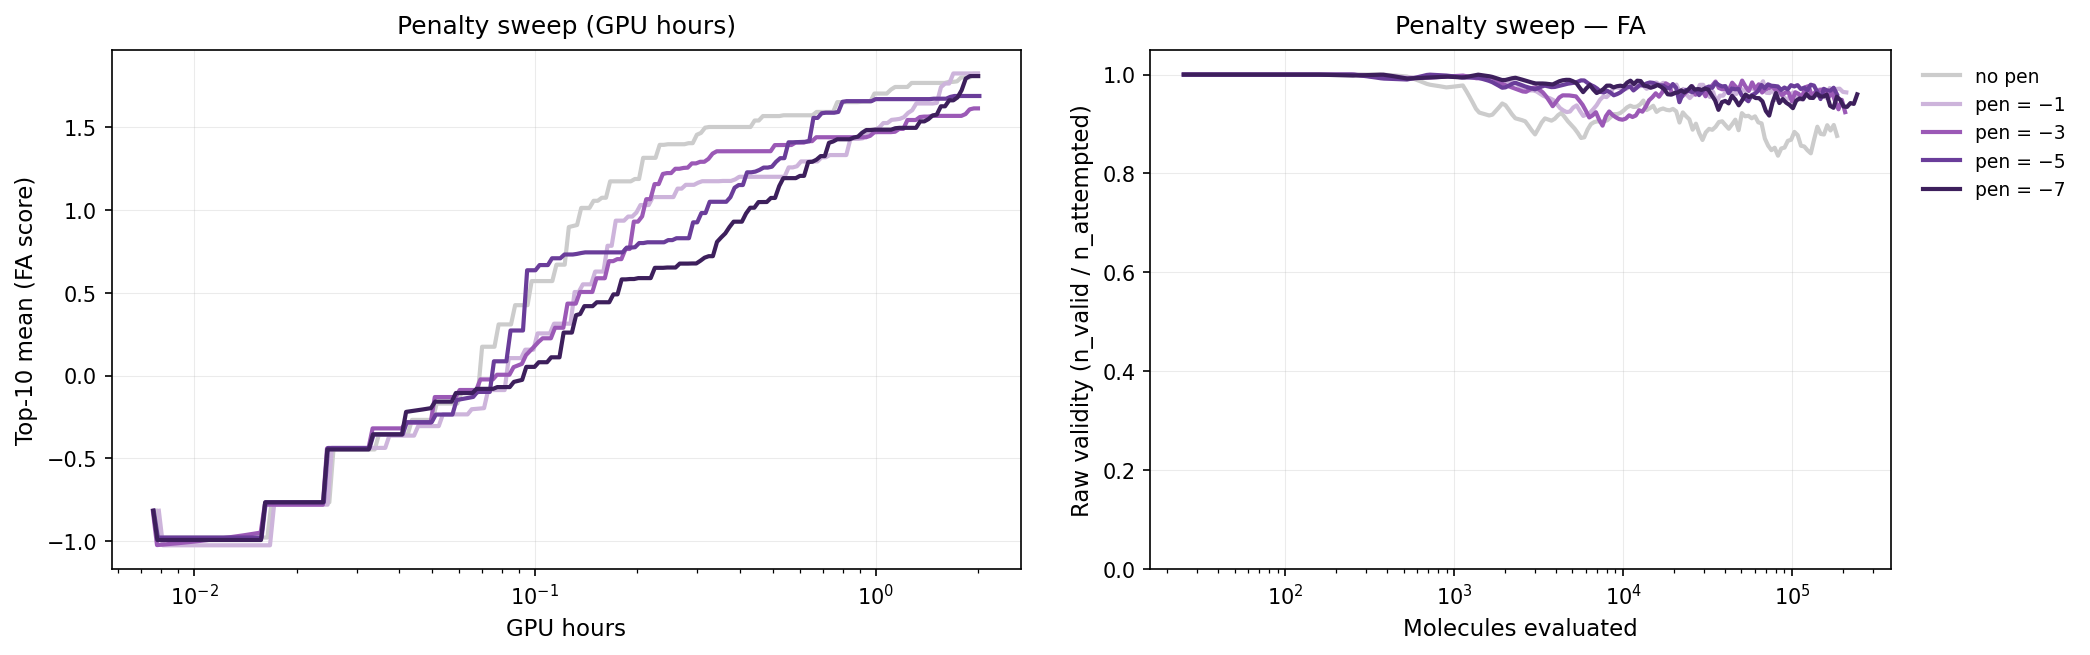
\includegraphics[width=0.85\textwidth]{figures/fig17_FA__b_h.png}
  \caption{Validity panel paired with top-1 FA for the same penalty sweep as Fig.~\ref{fig:penalty_ablation}, used in the body to motivate the choice of $r_{\text{inv}} = -5$. The $r_{\text{inv}}{=}0$ line shows grammar collapse; all non-zero penalties restore validity.}
  \label{fig:penalty_sweep}
\end{figure}

% Previous heading: \subsection{Per-family protein ablations} Table~\ref{tab:protein_knobs} reports the leave-one-out effect per protein family, which the aggregated protein panels of Fig.~\ref{fig:barplot_ablation} average over.
\subsubsection{Per-family protein ablations}
Table~\ref{tab:protein_knobs} reports the leave-one-out effect per protein family, which the aggregated protein panels of Fig.~\ref{fig:barplot_ablation} average over.

\begin{table}[H]
\centering
\small
\begin{tabular}{@{}lrrr@{}}
\toprule
\textbf{Component removed} & \textbf{GB1} & \textbf{TrpB} & \textbf{CreiLOV} \\
\midrule
Thompson acquisition   & $+1.038$ & $+0.279$ & $+0.090$ \\
CVaR shaping           & $+1.037$ & $+0.042$ & $+0.014$ \\
Replay buffer          & $+0.694$ & $+0.085$ & $+0.042$ \\
Density Entropy Reg.\  & $+0.179$ & $+0.035$ & $-0.184$ \\
Invalid-output penalty & $ 0.000$ & $-0.006$ & $ 0.000$ \\
\bottomrule
\end{tabular}
\caption{\textbf{Per-family leave-one-out effects on protein tasks.} Loss in best fitness from removing each component. Positive means the component helps. Only Thompson acquisition helps on all three families. The invalid-output penalty never fires: the protein sampler emits fixed-length sequences over the canonical amino acids, so invalid sequences cannot occur.}
\label{tab:protein_knobs}
\end{table}

The ordering is per-family rather than per-domain, and tracks prior coverage rather than modality. GB1 behaves like the small-molecule regime --- large gains from Thompson, CVaR, and replay --- and it is also the family whose prior is by far the least diverse, with only $35$ sequence clusters at $80\%$ identity in the training split against $33{,}851$ for TrpB and $185{,}774$ for CreiLOV. Density Entropy Regularization is the weakest knob throughout and turns negative on CreiLOV, which is what the prior-coverage account predicts: DER pushes sampling away from sequences the model already finds likely, and that pays off only when high-fitness sequences are ones the prior considers unlikely. Here the opposite holds --- scored under the frozen prior, high-fitness sequences are the \emph{more} typical ones on all three families (reward--NLL correlations $-0.24$ to $-0.74$) --- so pushing off-prior moves the search away from fitness.

% Previous heading: \subsection{Molecular length under Density Entropy Regularization}
\subsubsection{Molecular length under Density Entropy Regularization}
DER is not length-neutral for molecules. Table~\ref{tab:derlen} shows that the full method shifts evaluated candidates toward longer tokenized strings, especially early in the run, and that the shift persists within matched reward ranges, so it is not merely a by-product of reaching higher-reward regions.

\begin{table}[H]
\centering
\small
\begin{tabular}{@{}lrr@{}}
\toprule
\textbf{Window} & \textbf{Full (DER)} & \textbf{No-DER} \\
\midrule
First $20\%$ of oracle calls & $54.4$ & $39.4$ \\
Last $20\%$ of oracle calls  & $49.6$ & $41.2$ \\
\midrule
\multicolumn{3}{@{}l}{\textit{By FA reward range, last $20\%$}} \\
$<-2$        & $47.0$ & $39.4$ \\
$[-2,-1)$    & $41.1$ & $40.0$ \\
$[-1,0)$     & $45.1$ & $39.7$ \\
$[0,1)$      & $54.3$ & $43.9$ \\
$[1,2)$      & $57.5$ & $56.8$ \\
$\ge 2$      & $55.0$ & $41.9$ \\
\bottomrule
\end{tabular}
\caption{\textbf{Molecule token length under Density Entropy Regularization.} Mean tokenized SMILES length of oracle-evaluated candidates.}
\label{tab:derlen}
\end{table}

This does not by itself indicate a failure mode. DER is intended to improve top-molecule discovery, and the full method does find better top-scoring molecules. Length also \emph{decreases} from the first to the last $20\%$ of oracle calls ($54.4 \to 49.6$), so DER does not simply keep inflating length; it expands the searched molecular regime early and then shapes the sampling posterior within that regime. For proteins the mechanism does not apply at all, since sequence length is fixed by family.

% Previous heading: \subsection{Density estimator comparison}
\subsubsection{Density estimator comparison}
{\paragraph{Cheap estimator vs.\ LLaDA-Alg.\,3.}
We compare five density-entropy-regularization variants: the single-pass cheap estimator and LLaDA-Alg.\,3 with $n_{\text{mc}} \in \{1, 4, 8, 16\}$, for both DDPP-LB and VIDD on FA/2VT4. Fig.~\ref{fig:negscore_estimator_curves} shows best-so-far oracle score per oracle call and per GPU hour. The cheap estimator matches or exceeds all LLaDA variants on oracle-call efficiency and is substantially faster per GPU hour due to requiring only a single forward pass. Fig.~\ref{fig:negscore_nll_dist} shows the distribution of NLL under the pretrained model for the top-200 discovered molecules per variant, evaluated post-hoc via LLaDA-Alg.\,3 ($n_{\text{mc}}{=}32$). The cheap estimator induces at least as much off-prior shift as the LLaDA variants, confirming that the single-pass approximation is a computationally sound substitute.}

\begin{figure}[H]
  \centering
  {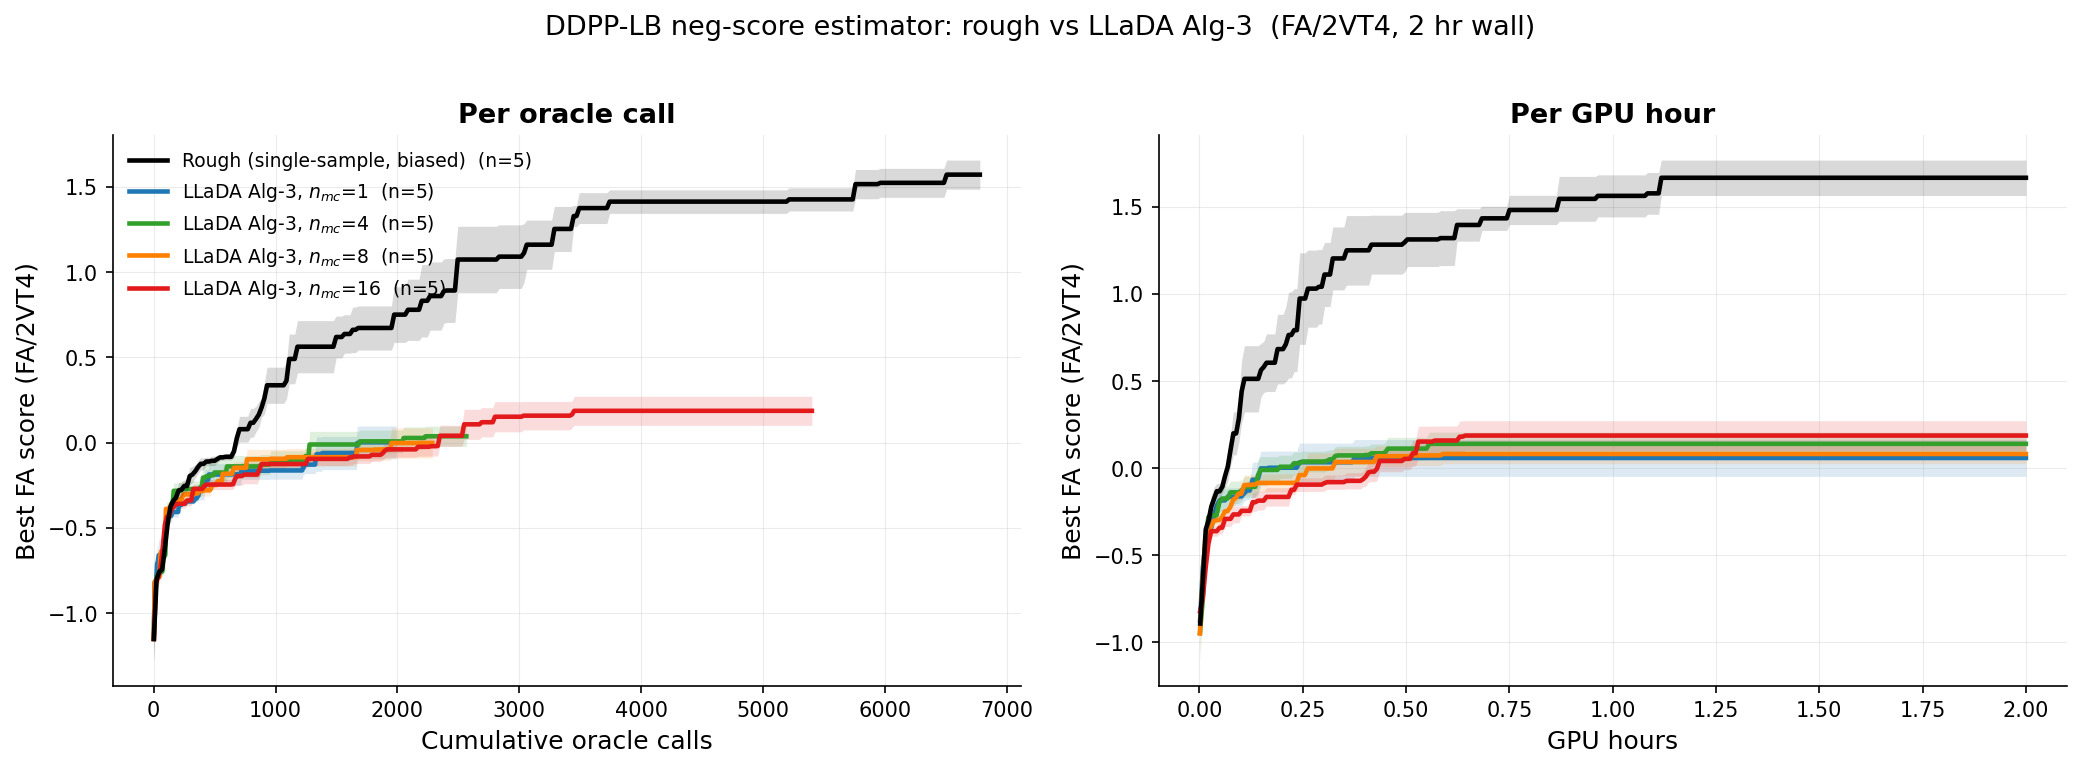
\includegraphics[width=\textwidth]{figures/negscore_estimator_ddpp.png}}\\[4pt]
  {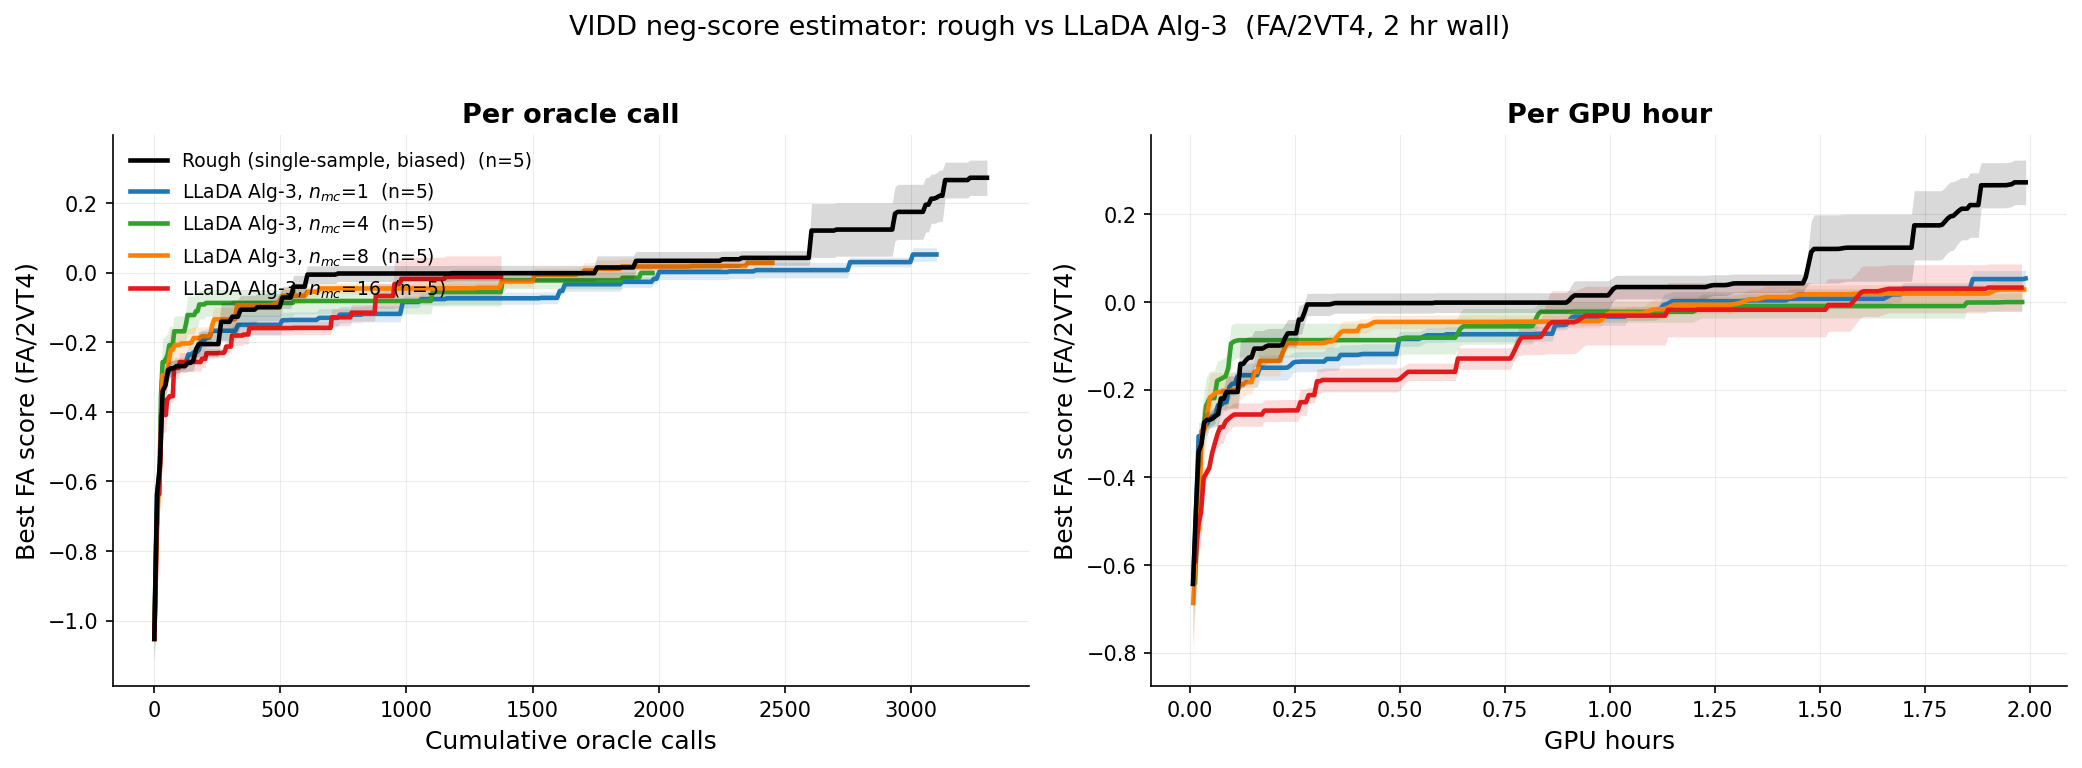
\includegraphics[width=\textwidth]{figures/negscore_estimator_vidd.png}}
  \caption{{\textbf{Best-so-far oracle curves: cheap estimator vs.\ LLaDA-Alg.\,3 variants (FA/2VT4, 2 hr wall).} Each subplot shows best FA score per oracle call (left) and per GPU hour (right) for five density-entropy-regularization variants: single-pass cheap estimator (black) and LLaDA-Alg.\,3 with $n_{\text{mc}} \in \{1,4,8,16\}$ (colored). \textbf{Top:} DDPP-LB. \textbf{Bottom:} VIDD. The cheap estimator matches or exceeds LLaDA variants on oracle calls and is far more or at least equally efficient per GPU hour.}}
  \label{fig:negscore_estimator_curves}
\end{figure}

\begin{figure}[H]
  \centering
  {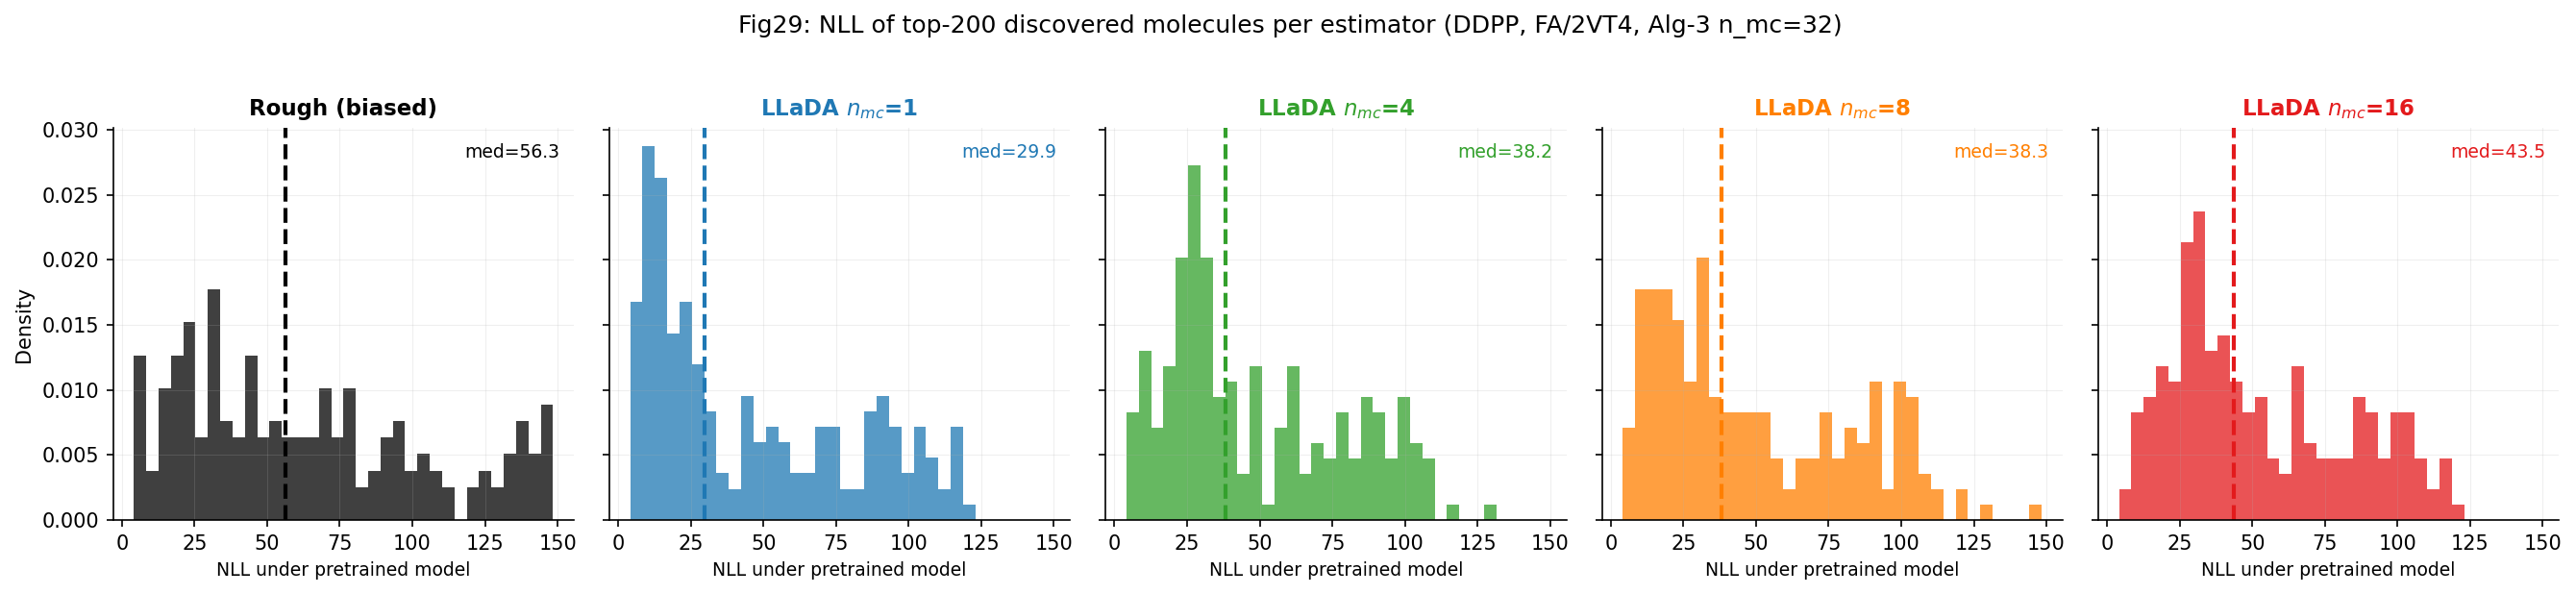
\includegraphics[width=\textwidth]{figures/negscore_nll_dist_ddpp.png}}\\[4pt]
  {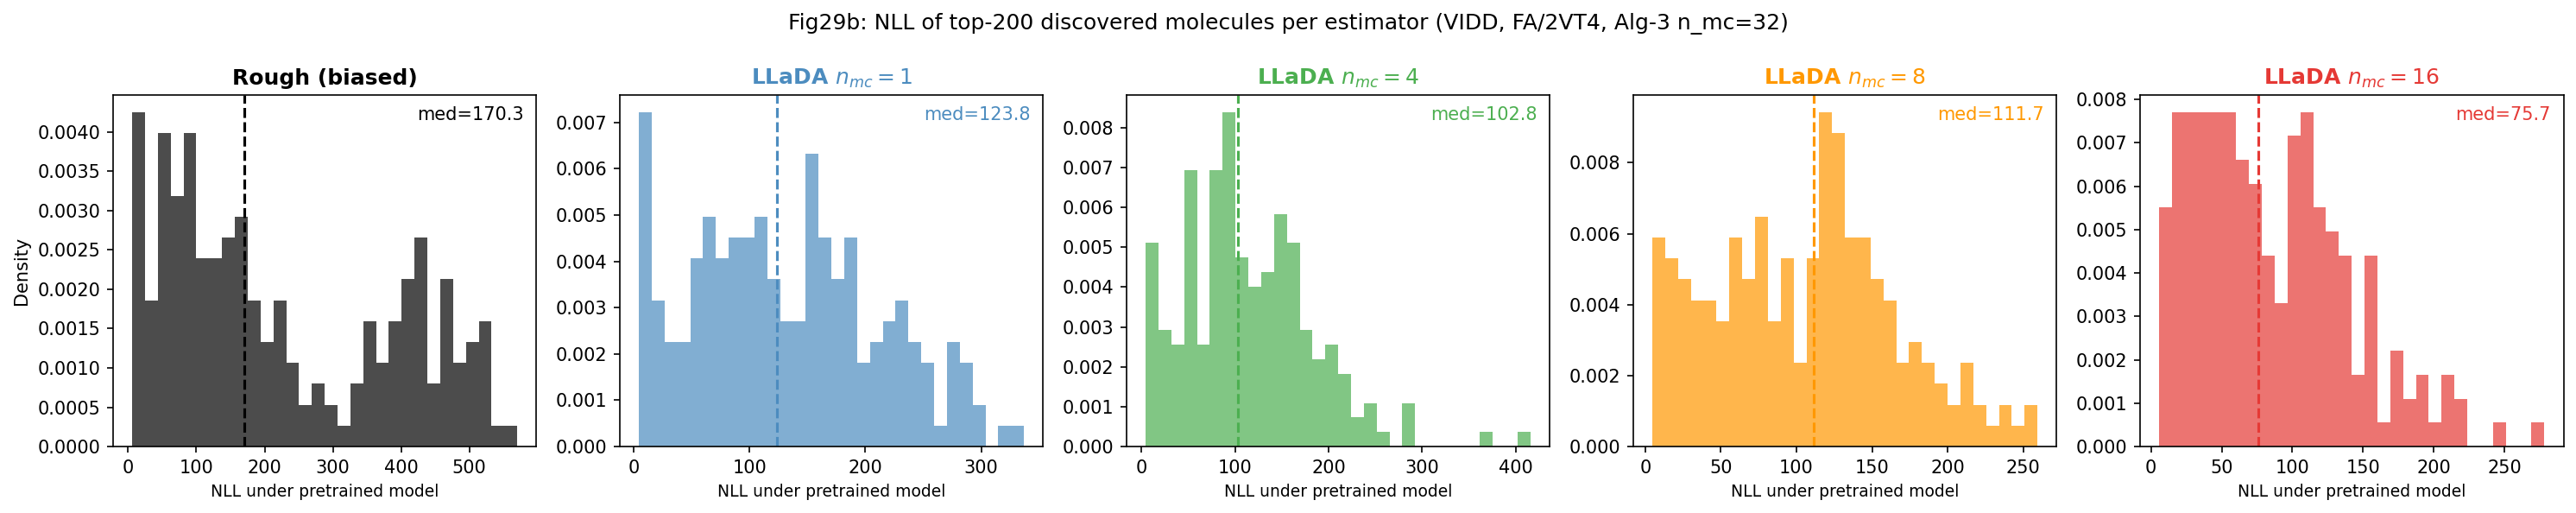
\includegraphics[width=\textwidth]{figures/negscore_nll_dist_vidd.png}}
  \caption{{\textbf{NLL under the pretrained model for the top-200 discovered molecules, per estimator (FA/2VT4).} NLL evaluated post-hoc via LLaDA-Alg.\,3 ($n_{\text{mc}}{=}32$); dashed line = median. \textbf{Top:} DDPP-LB. \textbf{Bottom:} VIDD. The cheap estimator produces distributions shifted at least as far off the prior as the LLaDA variants, validating that the single-pass approximation achieves the intended exploration pressure.}}
  \label{fig:negscore_nll_dist}
\end{figure}

% Previous heading: \section{Per-cell secondary-metric traces}\label{app:traces}
\subsection{Secondary Metrics and Distribution-Shift Diagnostics}\label{app:traces}

These panels report sliding-window means of pairwise Tanimoto diversity, QED, SA, and SMILES validity for the per-knob ablation cells of Appendix~\ref{app:knobs}. Window size 300, stride 200; one curve per cell, x-axis = molecules evaluated.

\begin{figure}[H]
  \centering
  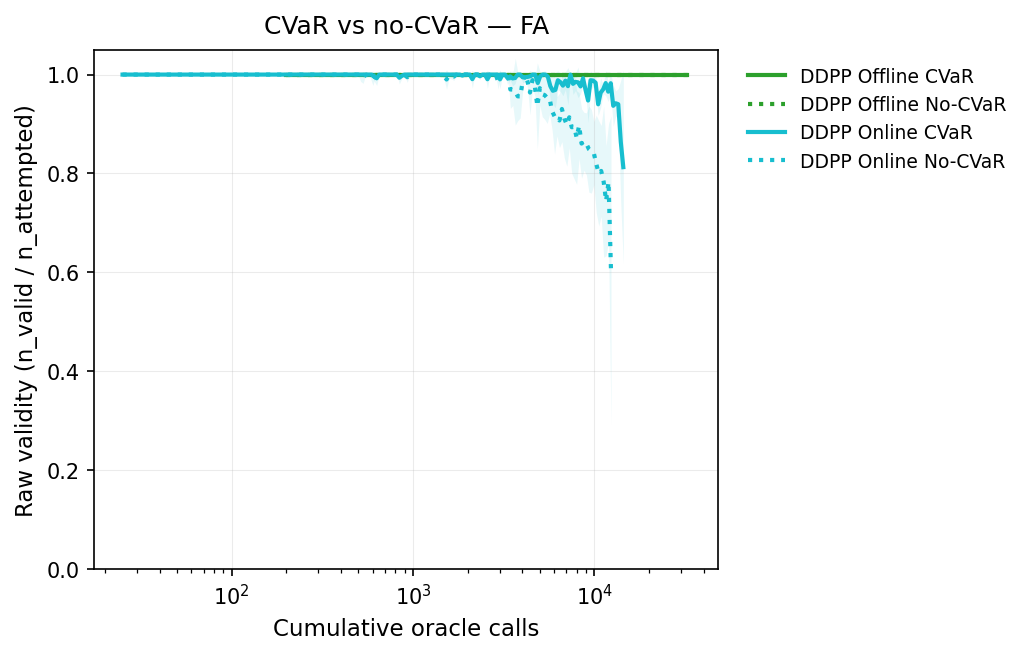
\includegraphics[width=0.49\textwidth]{figures/aux_rewardshape_validity.png}\hfill
  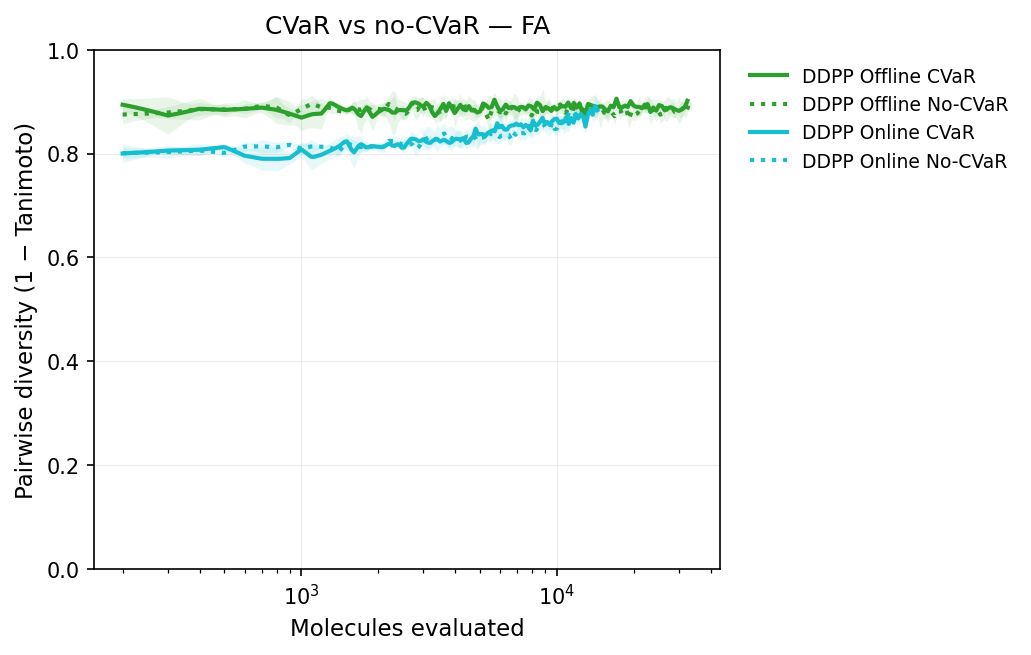
\includegraphics[width=0.49\textwidth]{figures/aux_rewardshape_tanimoto.png}\\[0.5ex]
  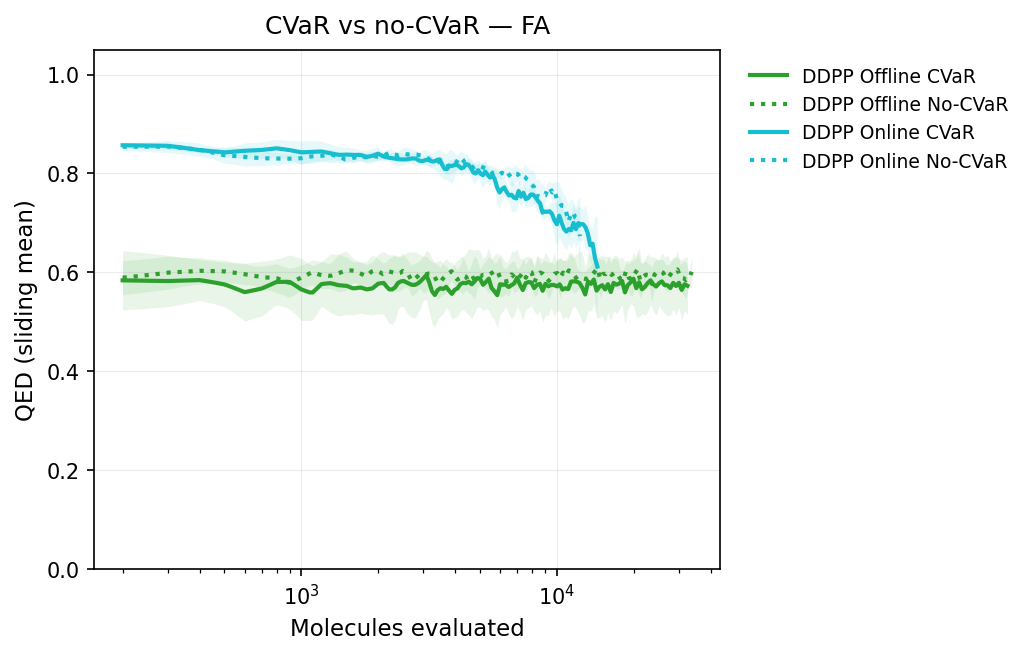
\includegraphics[width=0.49\textwidth]{figures/aux_rewardshape_qed.png}\hfill
  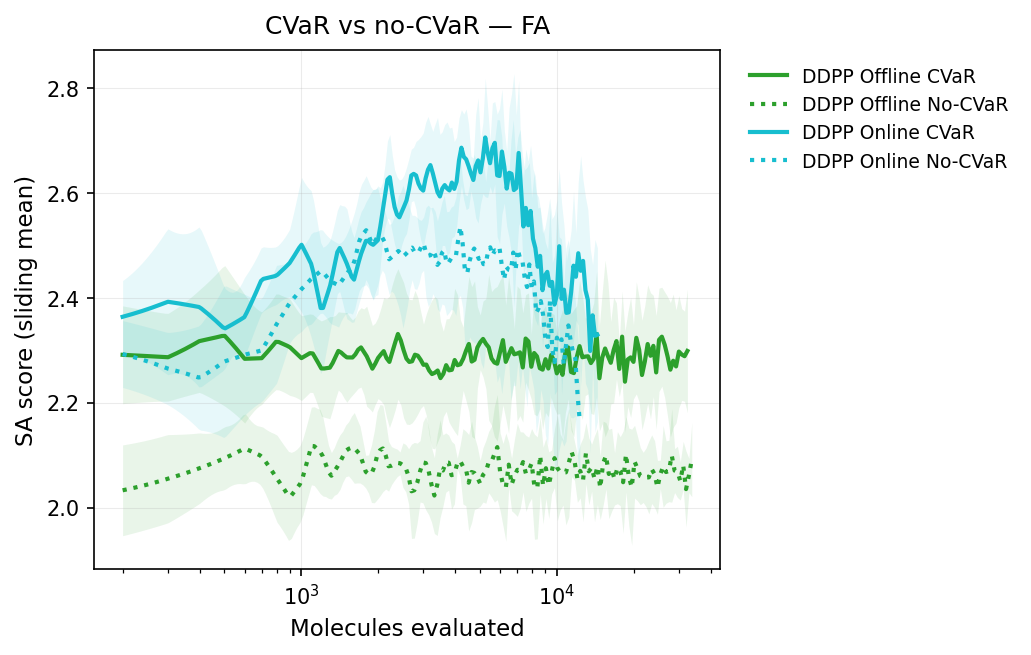
\includegraphics[width=0.49\textwidth]{figures/aux_rewardshape_sa.png}
  \caption{\textbf{CVaR ablation, secondary metrics.} Same four cells as Fig.~\ref{fig:cvar_ablation} (offline / online $\times$ CVaR-on / CVaR-off). Top-left: validity. Top-right: Tanimoto diversity. Bottom-left: QED. Bottom-right: SA. The top-1 FA gains in Fig.~\ref{fig:cvar_ablation} are not accompanied by validity collapse or QED/SA degradation, ruling out reward hacking on the CVaR knob.}
  \label{fig:traces_cvar}
\end{figure}

\begin{figure}[H]
  \centering
  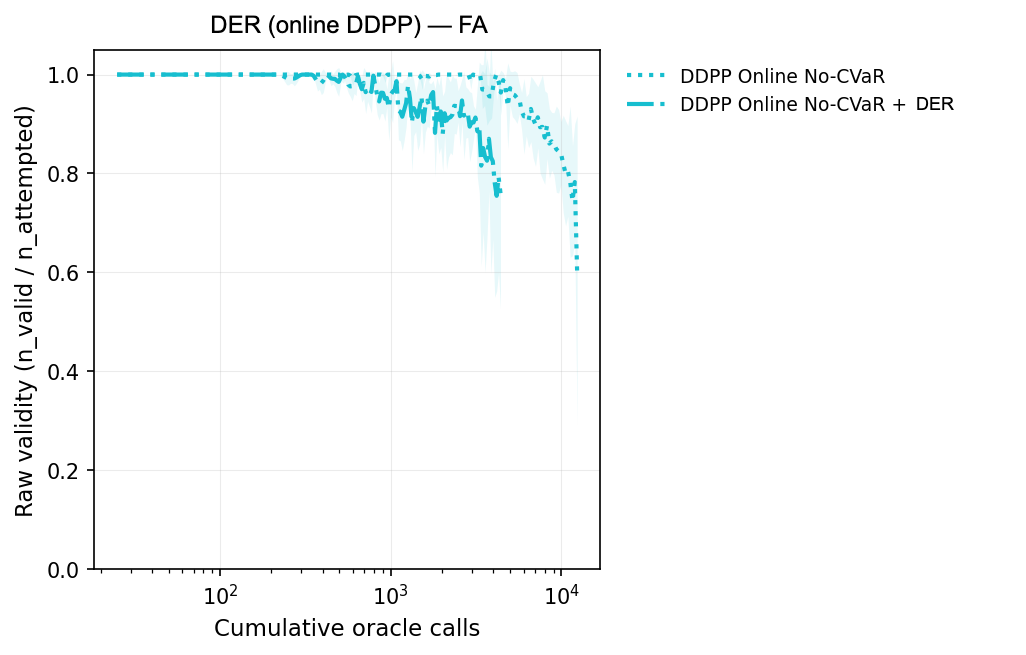
\includegraphics[width=0.49\textwidth]{figures/aux_debiasing_validity.png}\hfill
  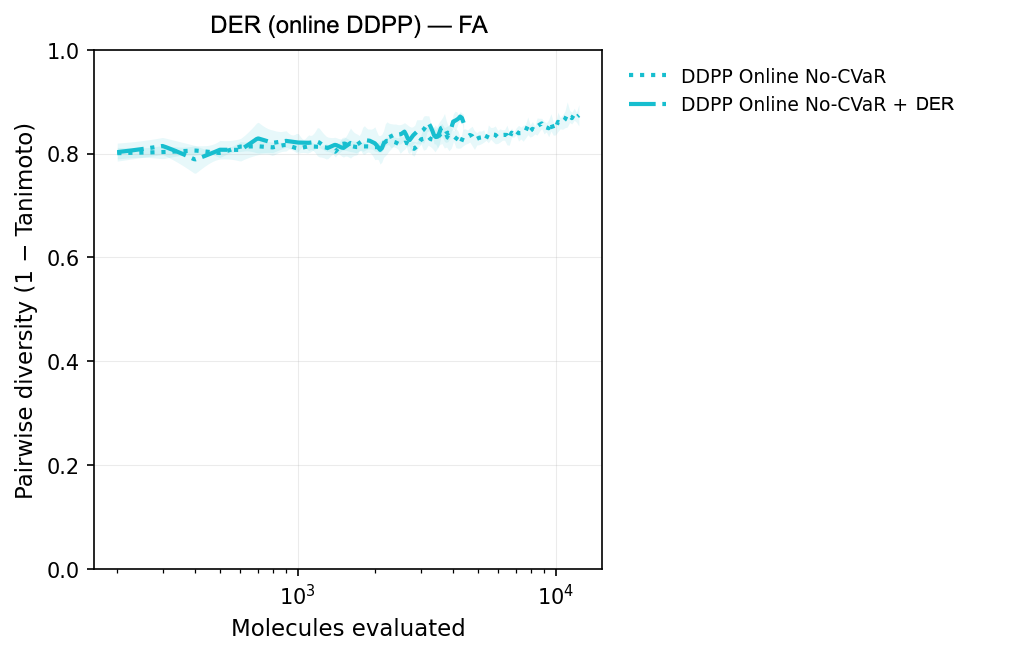
\includegraphics[width=0.49\textwidth]{figures/aux_debiasing_tanimoto.png}\\[0.5ex]
  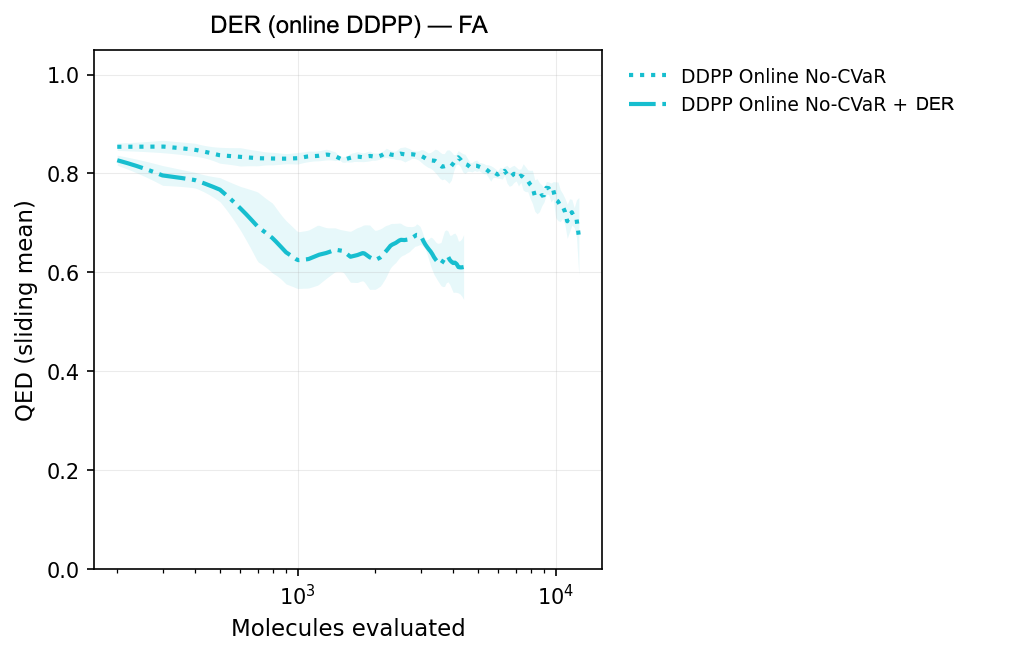
\includegraphics[width=0.49\textwidth]{figures/aux_debiasing_qed.png}\hfill
  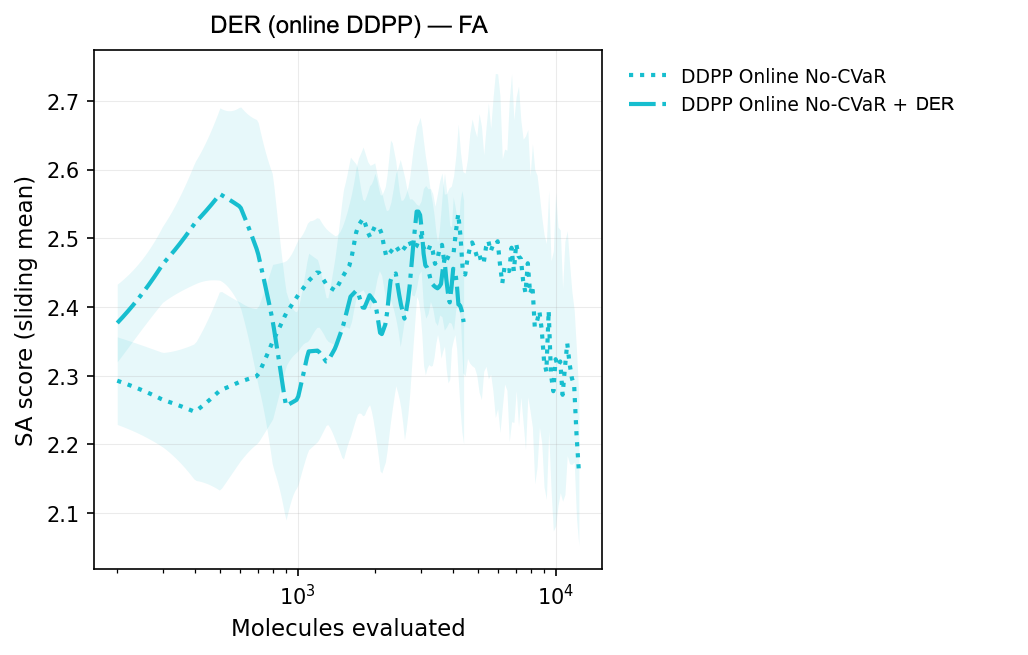
\includegraphics[width=0.49\textwidth]{figures/aux_debiasing_sa.png}
  \caption{\textbf{Model-debiasing ablation, secondary metrics.} Same two cells as Fig.~\ref{fig:debiasing_ablation} (online no-CVaR with vs.\ without Density Entropy Regularization). Same panel layout as above. The top-1 FA gain from debiasing is not accompanied by validity or QED/SA degradation.}
  \label{fig:traces_debiasing}
\end{figure}

\begin{figure}[H]
  \centering
  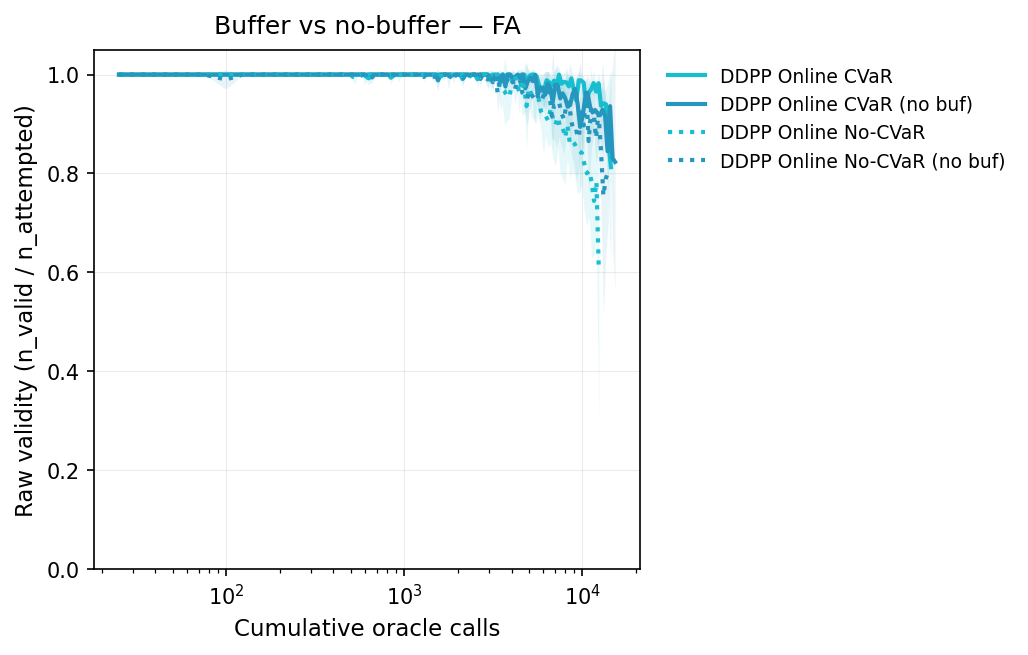
\includegraphics[width=0.49\textwidth]{figures/aux_buffer_validity.png}\hfill
  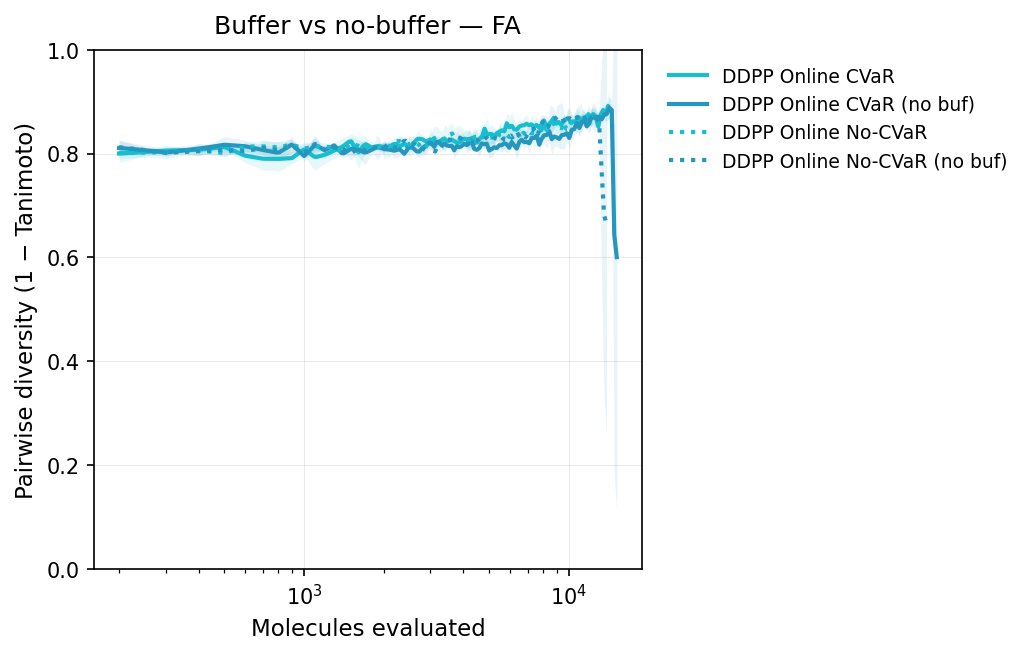
\includegraphics[width=0.49\textwidth]{figures/aux_buffer_tanimoto.png}\\[0.5ex]
  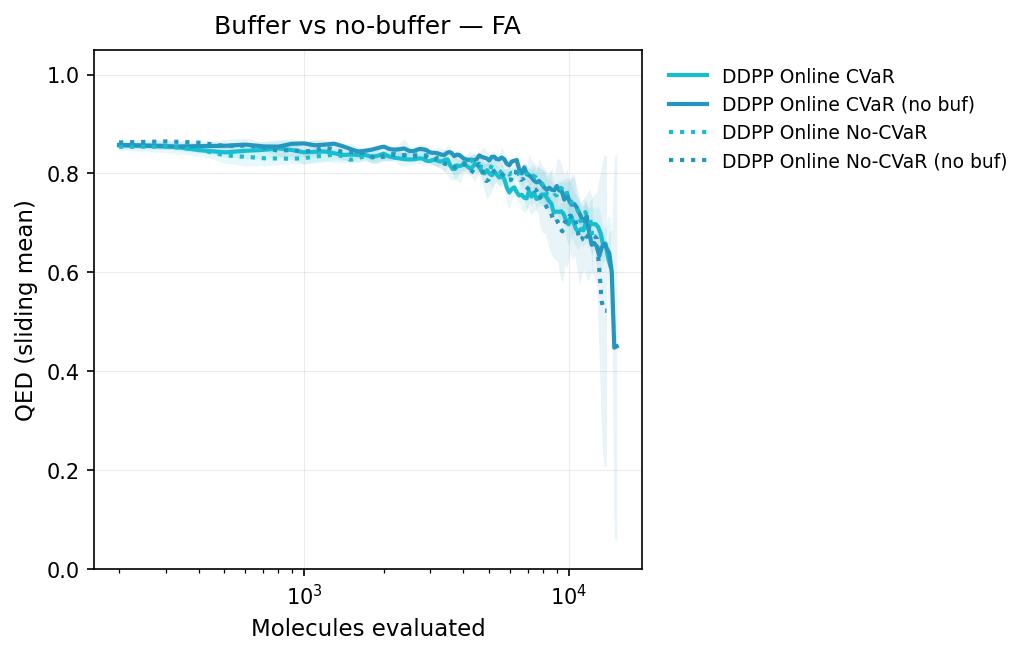
\includegraphics[width=0.49\textwidth]{figures/aux_buffer_qed.png}\hfill
  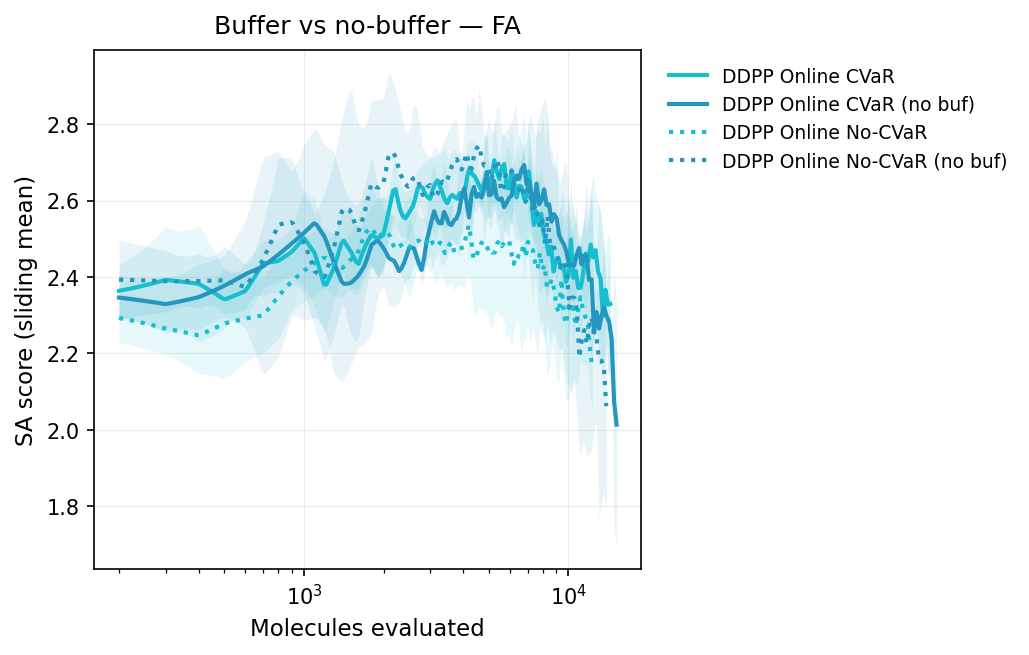
\includegraphics[width=0.49\textwidth]{figures/aux_buffer_sa.png}
  \caption{\textbf{Replay-buffer ablation, secondary metrics.} Same four cells as Fig.~\ref{fig:buffer_ablation} (buffer~$\times$~CVaR). Top-left: validity. Top-right: Tanimoto diversity. Bottom-left: QED. Bottom-right: SA. The buffer-on cells preserve diversity and SA more reliably than the buffer-off cells, consistent with the buffer's role as an implicit normalizer over the historical sample distribution (Sec.~\ref{sec:results}).}
  \label{fig:traces_buffer}
\end{figure}

The validity panel for the invalid-SMILES penalty sweep is reported directly in Fig.~\ref{fig:penalty_sweep}; per-cell QED/SA/Tanimoto for that sweep are not informative because the cells differ only in the validity-restoration penalty.

\paragraph{Run-end anchor-NLL distribution.} The per-knob traces above measure how the secondary metrics evolve over time. A complementary view is the end-of-run snapshot of how far each cell's policy $q_\theta$ has drifted from the frozen prior $p_{\text{pre}}$, measured by the anchor NLL $-\log p_{\text{pre}}(x_0 \mid x_t)$ averaged over masked tokens (Fig.~\ref{fig:anchor_nll}). Cells here are the leave-one-out variants from Section~\ref{sec:results} (full method minus one knob at a time), not the per-knob composition cells of Appendix~\ref{app:knobs}.

\begin{figure}[H]
  \centering
  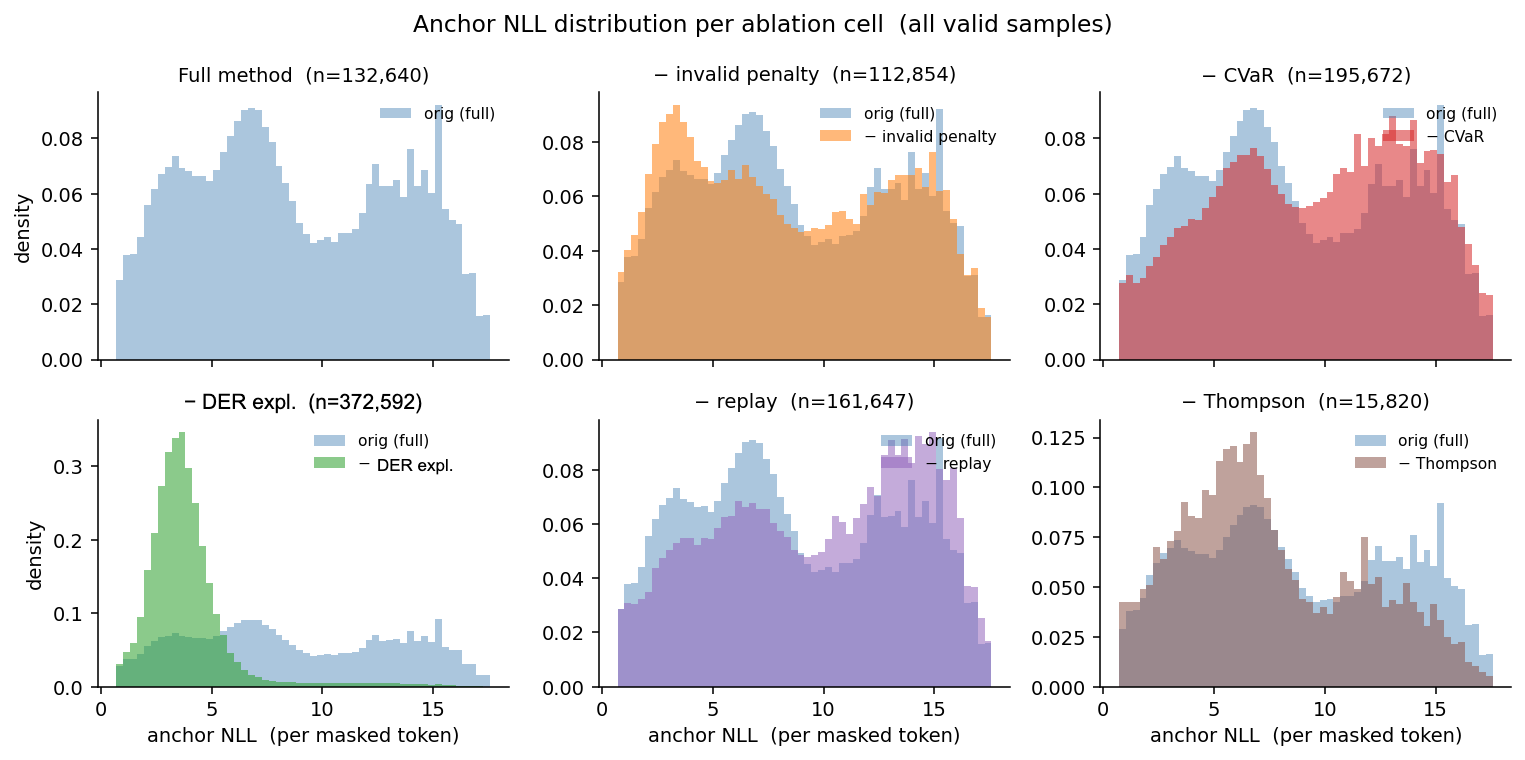
\includegraphics[width=\textwidth]{figures/anchor_nll_per_cell.png}
  \caption{\textbf{Anchor-NLL distribution per leave-one-out ablation cell.} Histogram of per-token anchor NLL $-\log p_{\text{pre}}(x_0 \mid x_t)$ at run end, computed over all valid samples (n in title). Top-left is the full method; the other five panels each remove one knob and overlay the resulting distribution against the full-method reference (blue). Removing the density entropy regularization / debiasing knob (bottom-left) collapses mass back toward the prior (low anchor NLL) far more than removing any other knob, identifying debiasing as the primary driver of distribution shift away from $p_{\text{pre}}$. Removing CVaR (top-right) reduces the high-NLL tail, consistent with CVaR's role in pushing the policy toward the upper-reward region of the distribution. The remaining knobs (invalid penalty, replay buffer, Thompson) leave the bimodal shape qualitatively intact.}
  \label{fig:anchor_nll}
\end{figure}

% Previous heading: \section{Multi-knob ablation: DER; CVaR; Thompson Sampling}\label{app:factorial}
\subsection{Joint Component Effects and the Untreated Baseline}\label{app:factorial}

Table~\ref{tab:factorial} in the main text reports the complete $2\times2\times2$ factorial over Density Entropy Regularization (DER), CVaR shaping, and Thompson acquisition. Leave-one-out ablations alone cannot separate additivity from redundancy, because they measure only the marginal effect of removing a component from the full configuration; the factorial resolves this.

% Duplicate of the main-text factorial table; retained below for recovery.
% \begin{table}[H]
% \centering
% \small
% \begin{tabular}{@{}cccr@{}}
% \toprule
% DER & CVaR & Thompson & Score \\
% \midrule
% on  & on  & on  & $+1.13$ \\
% on  & off & on  & $+0.54$ \\
% on  & on  & off & $-0.20$ \\
% on  & off & off & $-0.43$ \\
% off & on  & on  & $-0.54$ \\
% off & off & on  & $-0.80$ \\
% off & on  & off & $-0.86$ \\
% off & off & off & $-1.06$ \\
% \bottomrule
% \end{tabular}
% \caption{\textbf{All eight combinations of DER, CVaR, and Thompson (DDPP-LB).} Mean best oracle score at $1{,}000$ oracle calls, averaged over $30$ target--seed pairs. Turned on alone from the all-off cell, DER is worth $+0.63$, Thompson $+0.26$, and CVaR $+0.20$.}
% \label{tab:factorial-appendix}
% \end{table}

The components are neither purely additive nor redundant. DER acts as a gate: with DER off, all four cells sit between $-1.06$ and $-0.54$ regardless of what CVaR and Thompson do, whereas with DER on those same two knobs move the score from $-0.43$ to $+1.13$. CVaR's marginal value is $+0.20$ with DER and Thompson both off, $+0.26$ with Thompson on but DER off, and $+0.59$ with DER on; Thompson shows the same pattern. No component's marginal value falls to zero given the others, which rules out redundancy. This is the operational sense of \emph{complementary} used in Sec.~\ref{sec:results-method}: each component's marginal value depends on which others are active, and that dependence is positive. The pattern is consistent with the distribution-shift analysis of Sec.~\ref{sec:analysis} --- CVaR and Thompson concentrate effort on the upper tail of whatever region the generator currently occupies, so if the policy has not been pushed off the prior's dominant modes there is little tail to concentrate on, and DER is what opens that headroom.

\paragraph{Comparison against the untreated (all-knobs-off) baseline.} Table~\ref{tab:allknobs} compares the full harness against the untreated online DDPP-LB configuration defined in Sec.~\ref{sec:exp-setup}, at a matched budget of $4{,}000$ oracle calls.

\begin{table}[H]
\centering
\small
\begin{tabular}{@{}lrrrrr@{}}
\toprule
 & \textbf{Best} & \textbf{Top-10} & \textbf{Top-100} & \textbf{Median} & \textbf{Mean of all} \\
\midrule
All five knobs on  & $+1.15$ & $+0.89$ & $+0.46$ & $-0.96$ & $-1.09$ \\
All five knobs off & $-0.49$ & $-0.73$ & $-1.55$ & $-2.65$ & $-2.66$ \\
\bottomrule
\end{tabular}
\caption{\textbf{Full harness vs.\ the untreated all-knobs-off baseline (DDPP-LB).} Averaged over $3$ targets at $4{,}000$ oracle calls. The measured top-$100$ gap of $+2.01$ is roughly $7\times$ the mean within-cell standard deviation.}
\label{tab:allknobs}
\end{table}

The gap is not a transient early advantage that more oracle calls would close: the untreated baseline never improves. Averaging the score of newly sampled molecules over successive blocks of $1{,}000$ calls gives $-2.68$, $-2.67$, $-2.65$, $-2.65$ for the all-off configuration against $-1.40$, $-0.94$, $-1.00$, $-1.06$ for the full method, so the all-off block mean is flat across the whole run while the full method rises. On 2VT4 specifically the same per-block comparison gives $-1.21$, $-1.23$, $-1.22$, $-1.22$ for all-off against $+0.10$, $+0.32$, $+0.25$, $+0.22$ for the full configuration.

\begin{figure}[ht]
    \centering
    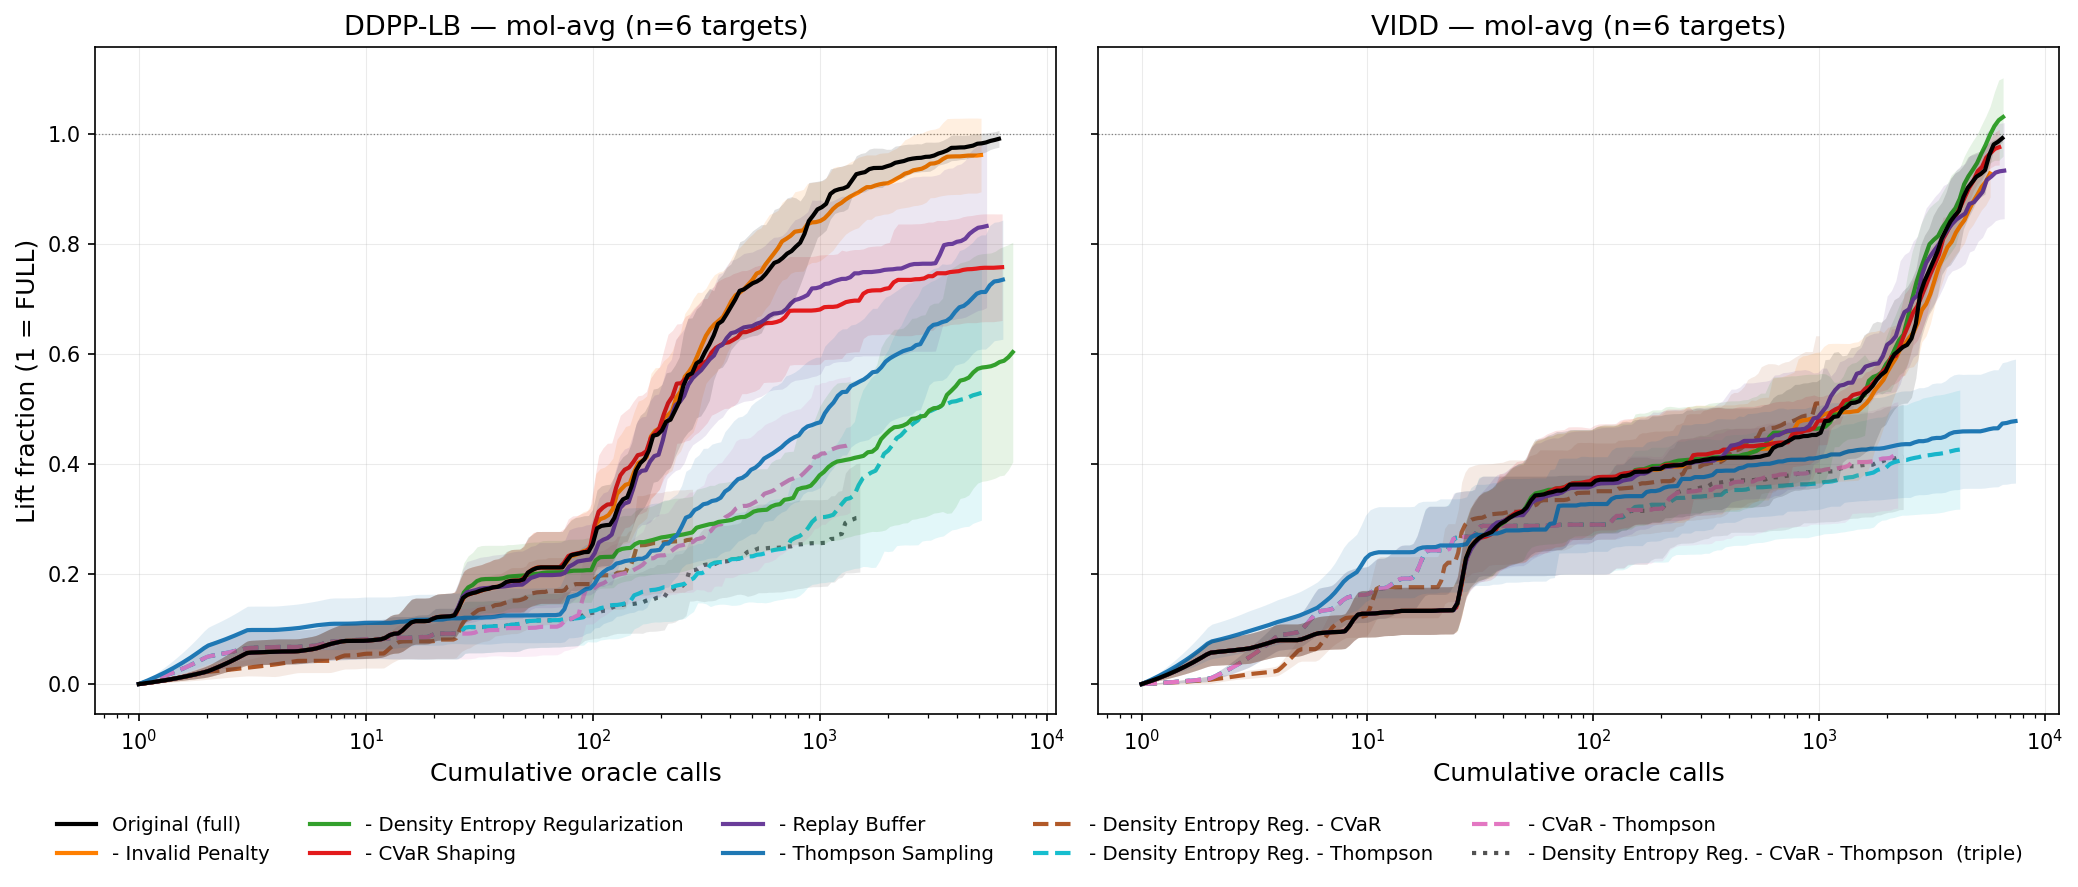
\includegraphics[width=\linewidth]{figures/ablations/multiknob_ablation_lift_curves.png}
    \caption{\textbf{Multi-knob ablation: normalised-reward trajectories.} Normalised reward ($1=$ FULL final) vs.\ cumulative oracle calls, averaged across the six FA-oracle small-molecule targets and five seeds; pair removals dashed, triple removal dotted. Removing additional exploration / shaping knobs degrades lift roughly monotonically the triple sits lowest at every budget on DDPP-LB, with VIDD showing the same ordering at compressed spread.}
    \label{fig:multiknob_lift_curves}
\end{figure}

\begin{figure}[ht]
    \centering
    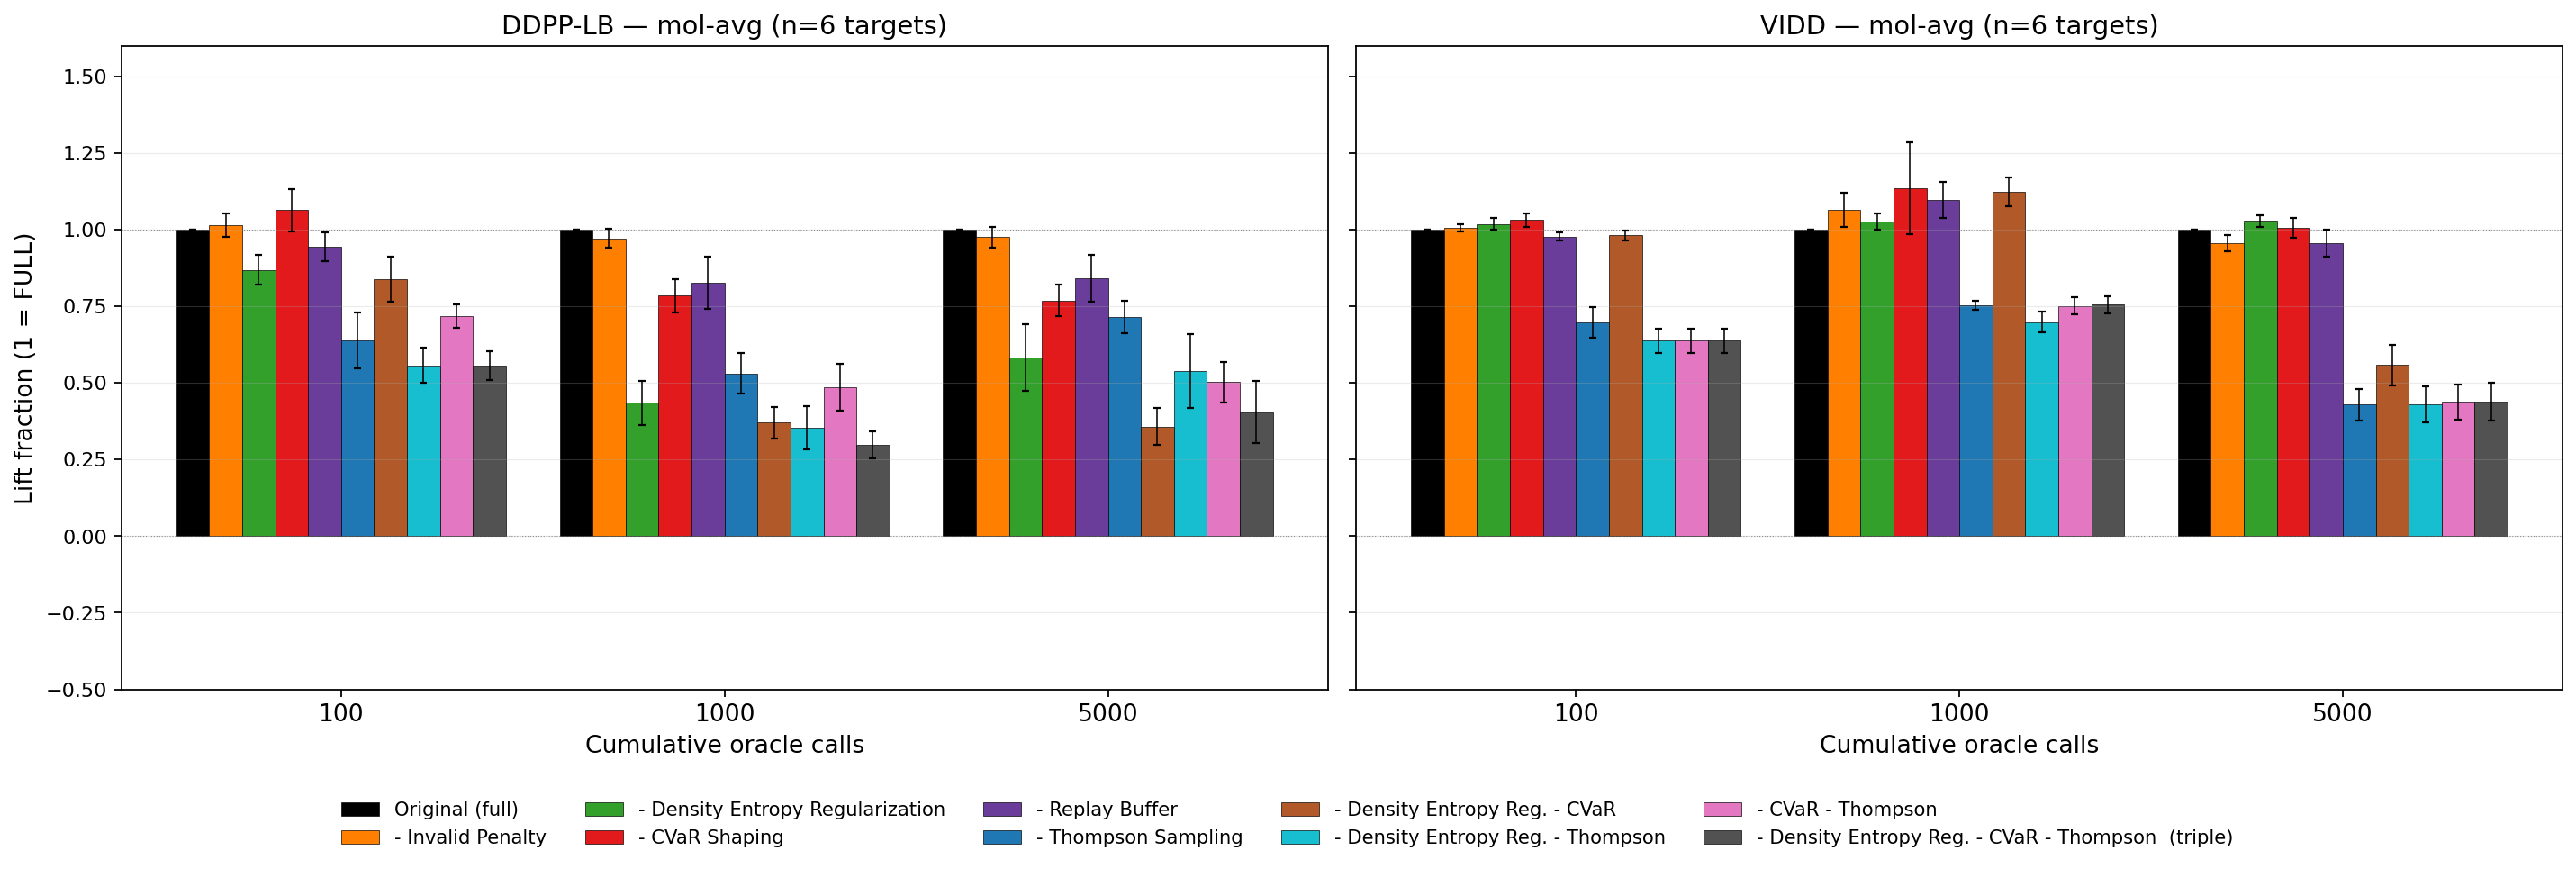
\includegraphics[width=\linewidth]{figures/ablations/multiknob_ablation_lift_bars.png}
    \caption{\textbf{Multi-knob ablation: normalised reward at oracle-call slices.} Same normalization as Fig.~\ref{fig:barplot_ablation}; six FA-oracle targets averaged, error bars $\pm 1$ SEM across targets. No pair removal sits above either of its constituent single removals at the 5\,000-call slice joint losses compound rather than substitute.}
    \label{fig:multiknob_lift_bars}
\end{figure}

\begin{figure}[ht]
    \centering
    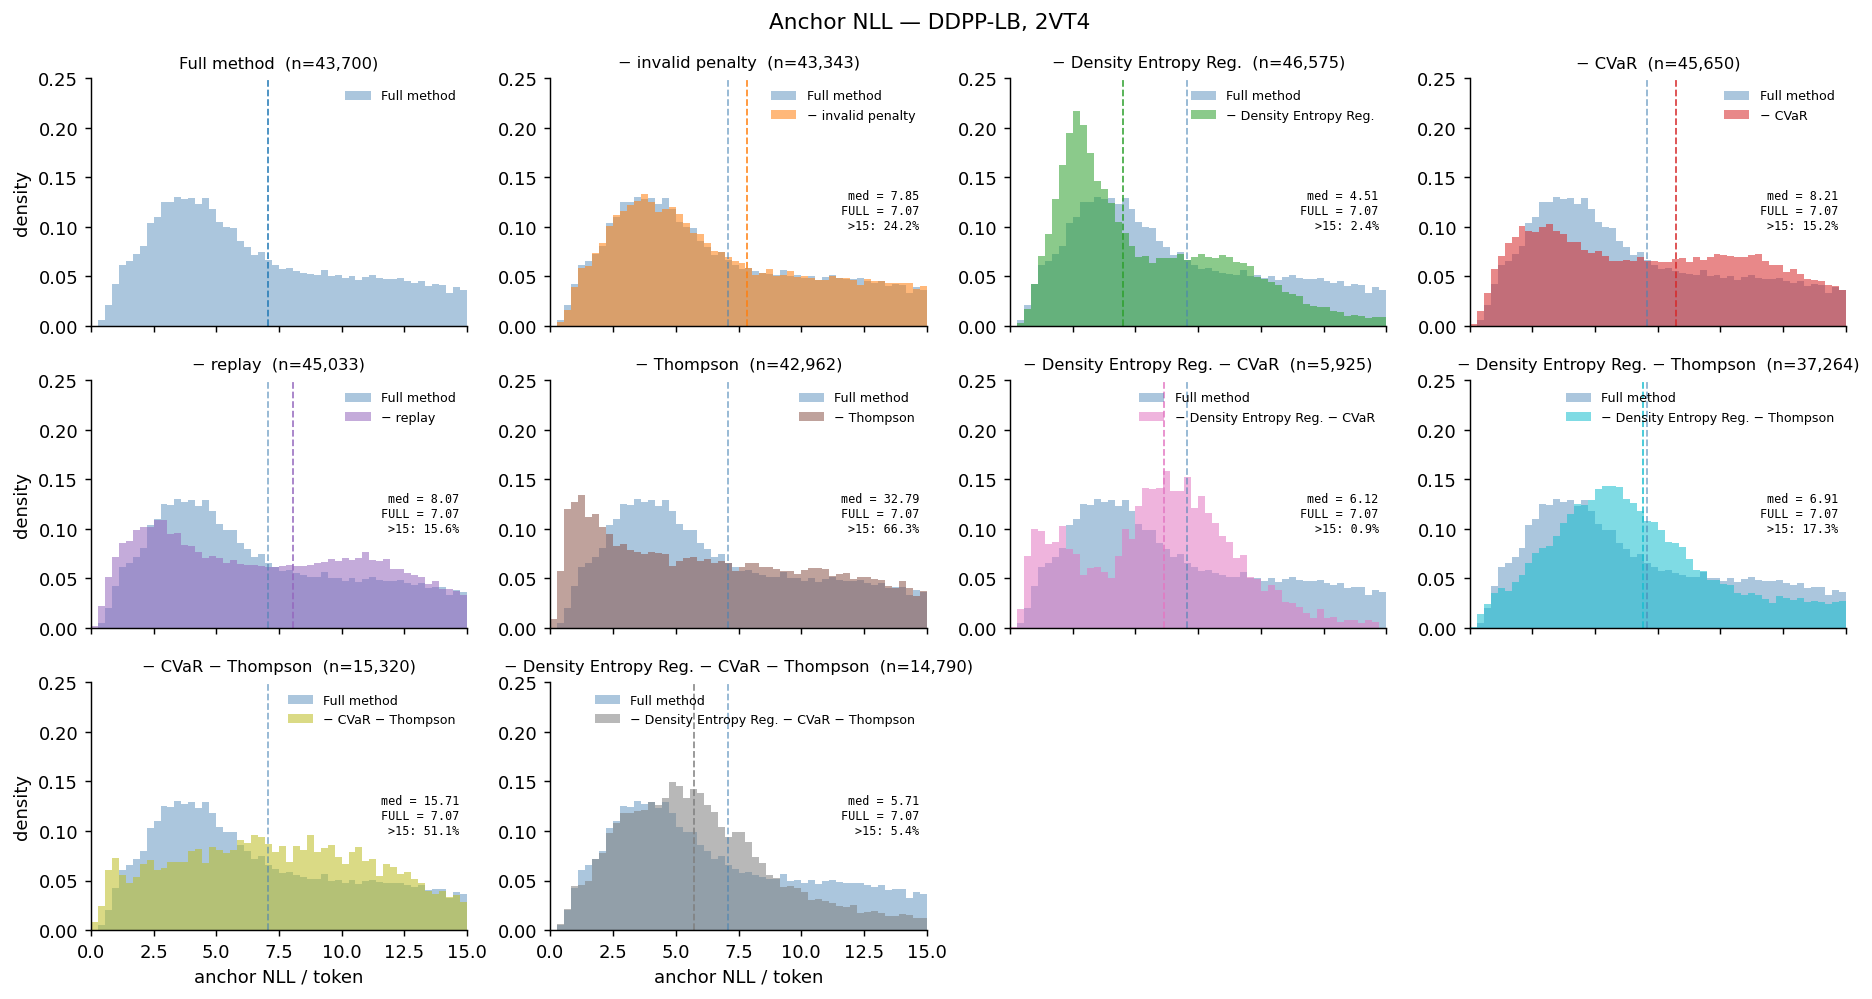
\includegraphics[width=\linewidth]{figures/ablations/multiknob_ablation_anchor_nll_2vt4_ddpp.png}
    \caption{\textbf{Anchor-NLL distribution per multi-knob ablation cell (DDPP-LB, 2VT4).} Per-token anchor NLL $-\log p_{\text{pre}}(x_0 \mid x_t)$ under the frozen pretrained generator on all oracle-evaluated SMILES (5 seeds), rough estimator with $T=10$ random-mask MC averaging; FULL (steelblue) overlaid as reference. Every cell with Density Entropy Regularization removed collapses mass back toward the prior, identifying DE as the dominant driver of distribution shift away from $p_{\text{pre}}$ regardless of the other knobs.}
    \label{fig:multiknob_anchor_nll}
\end{figure}

\clearpage

% Previous heading: \section{Cross-finetuner ablations: DDPP-LB and VIDD}\label{app:vidd-ablation}
\subsection{Cross-Finetuner Ablations: DDPP-LB and VIDD}\label{app:vidd-ablation}

% Previous heading: \subsection{Numerical summary across tasks}
\subsubsection{Numerical summary across tasks}

\begin{table}[t]
\centering
\footnotesize
\setlength{\tabcolsep}{4.5pt}
\caption{\textbf{Ablation normalised reward (mean $\pm$ s.e.).} Each row removes one design choice from the full method. Values are averaged across 6 molecular targets (Mol) and 3 protein families (Prot), normalised by the per-target range $[C_t, F_t]$ shared with the bar chart in Fig.~\ref{fig:barplot_ablation}.}
\label{tab:ablation_numbers}
\begin{tabular}{@{}lrcccc@{}}
\toprule
 & & \multicolumn{2}{c}{\textbf{DDPP}} & \multicolumn{2}{c}{\textbf{VIDD}} \\
\cmidrule(lr){3-4}\cmidrule(lr){5-6}
\textbf{Ablation} & \textbf{Calls} & \textbf{Mol} & \textbf{Prot} & \textbf{Mol} & \textbf{Prot} \\
\midrule
\multirow{3}{*}{Full method}
  & 100   & $.25{\pm}.02$ & $.72{\pm}.03$ & $.41{\pm}.03$ & $.66{\pm}.05$ \\
  & 1k    & $.85{\pm}.02$ & $.91{\pm}.01$ & $.49{\pm}.03$ & $.79{\pm}.04$ \\
  & 5k    & $.97{\pm}.01$ & $.94{\pm}.01$ & $.89{\pm}.02$ & $.87{\pm}.03$ \\
\midrule
\multirow{3}{*}{$-$ Invalid Pen.}
  & 100   & $.26{\pm}.02$ & $.72{\pm}.03$ & $.41{\pm}.03$ & $.66{\pm}.05$ \\
  & 1k    & $.83{\pm}.02$ & $.90{\pm}.01$ & $.51{\pm}.03$ & $.79{\pm}.04$ \\
  & 5k    & $.94{\pm}.02$ & $.95{\pm}.02$ & $.86{\pm}.03$ & $.87{\pm}.03$ \\
\midrule
\multirow{3}{*}{$-$ CVaR Shaping}
  & 100   & $.27{\pm}.02$ & $.72{\pm}.03$ & $.42{\pm}.02$ & $.67{\pm}.04$ \\
  & 1k    & $.67{\pm}.03$ & $.83{\pm}.03$ & $.51{\pm}.02$ & $.82{\pm}.03$ \\
  & 5k    & $.75{\pm}.03$ & $.85{\pm}.03$ & $.90{\pm}.03$ & $.90{\pm}.02$ \\
\midrule
\multirow{3}{*}{$-$ Density Entr.\ Reg.}
  & 100   & $.22{\pm}.01$ & $.77{\pm}.03$ & $.41{\pm}.02$ & $.66{\pm}.05$ \\
  & 1k    & $.39{\pm}.04$ & $.89{\pm}.01$ & $.49{\pm}.03$ & $.76{\pm}.04$ \\
  & 5k    & $.57{\pm}.04$ & $.97{\pm}.01$ & $.91{\pm}.02$ & $.84{\pm}.03$ \\
\midrule
\multirow{3}{*}{$-$ Replay Buffer}
  & 100   & $.24{\pm}.02$ & $.72{\pm}.03$ & $.41{\pm}.03$ & $.65{\pm}.05$ \\
  & 1k    & $.71{\pm}.03$ & $.83{\pm}.02$ & $.51{\pm}.03$ & $.85{\pm}.02$ \\
  & 5k    & $.82{\pm}.04$ & $.87{\pm}.02$ & $.85{\pm}.03$ & $.97{\pm}.01$ \\
\midrule
\multirow{3}{*}{$-$ Thompson Samp.}
  & 100   & $.18{\pm}.02$ & $.72{\pm}.03$ & $.31{\pm}.02$ & $.58{\pm}.04$ \\
  & 1k    & $.47{\pm}.03$ & $.78{\pm}.02$ & $.39{\pm}.02$ & $.66{\pm}.05$ \\
  & 5k    & $.70{\pm}.03$ & $.82{\pm}.01$ & $.44{\pm}.03$ & $.71{\pm}.04$ \\
\bottomrule
\end{tabular}
\end{table}


% Previous heading: \subsection{Per-task VIDD trajectories}
\subsubsection{Per-task VIDD trajectories}

\begin{figure}[H]
  \centering
  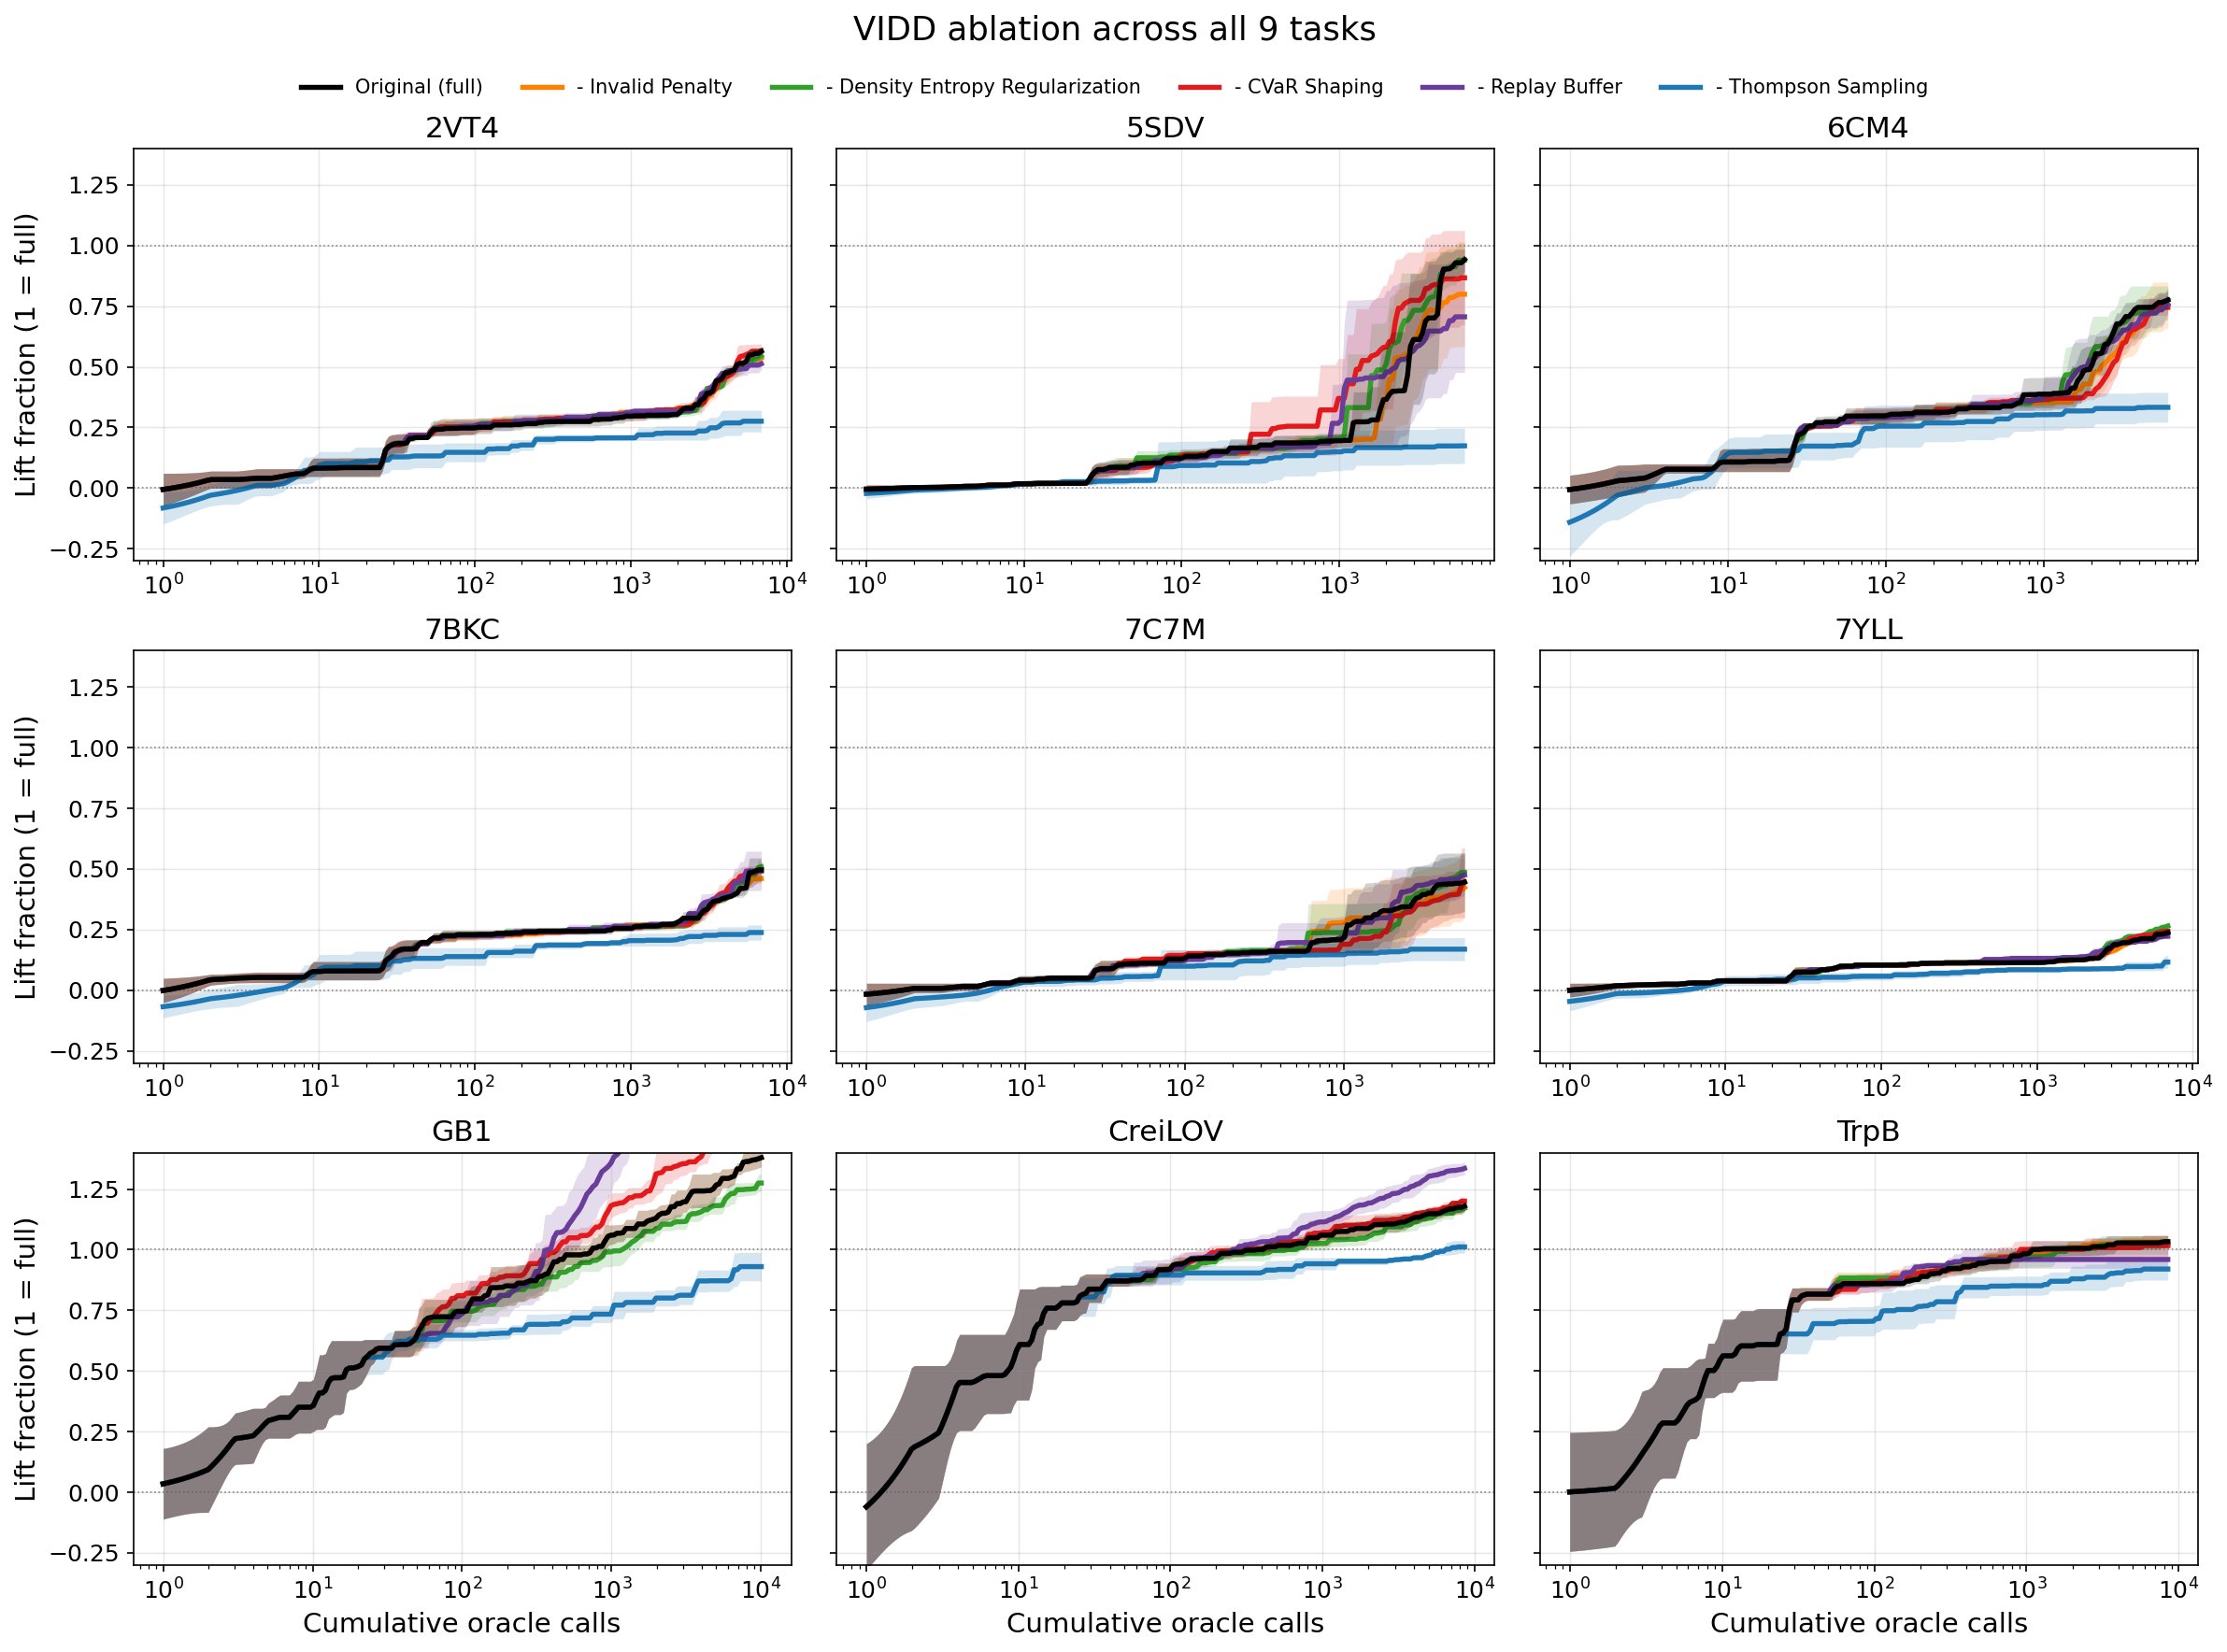
\includegraphics[width=0.95\textwidth]{figures/ablations/vidd_only_grid_norm.png}
  \caption{\textbf{VIDD harness ablation across all $9$ tasks.} Mirror of Fig.~\ref{fig:ablation_ddpp} with VIDD substituted for DDPP-LB as the finetuning objective $\mathcal{L}_{\text{ft}}$ in the harness; normalised reward is per-target $(1 =$ full VIDD$)$. Knob ordering matches DDPP-LB on most targets, supporting the harness claim of Sec.~\ref{sec:design-space} that knob intent transfers across finetuners. Spread between ablation cells is consistently smaller under VIDD: the student-teacher distillation step damps the policy drift that the exploration / objective-mismatch knobs amplify under DDPP-LB, so each knob's marginal contribution is also damped.}
  \label{fig:ablation_vidd}
\end{figure}

\clearpage

% Previous heading: \section{Search comparisons and compute breakdowns}\label{app:search}
\section{Search Baselines and Compute Accounting}\label{app:search}

This section separates comparisons of optimization strategies from their computational cost. Each performance comparison reports both cumulative oracle calls and GPU hours.

\subsection{Online adaptation and search baselines}

\begin{figure}[H]
  \centering
  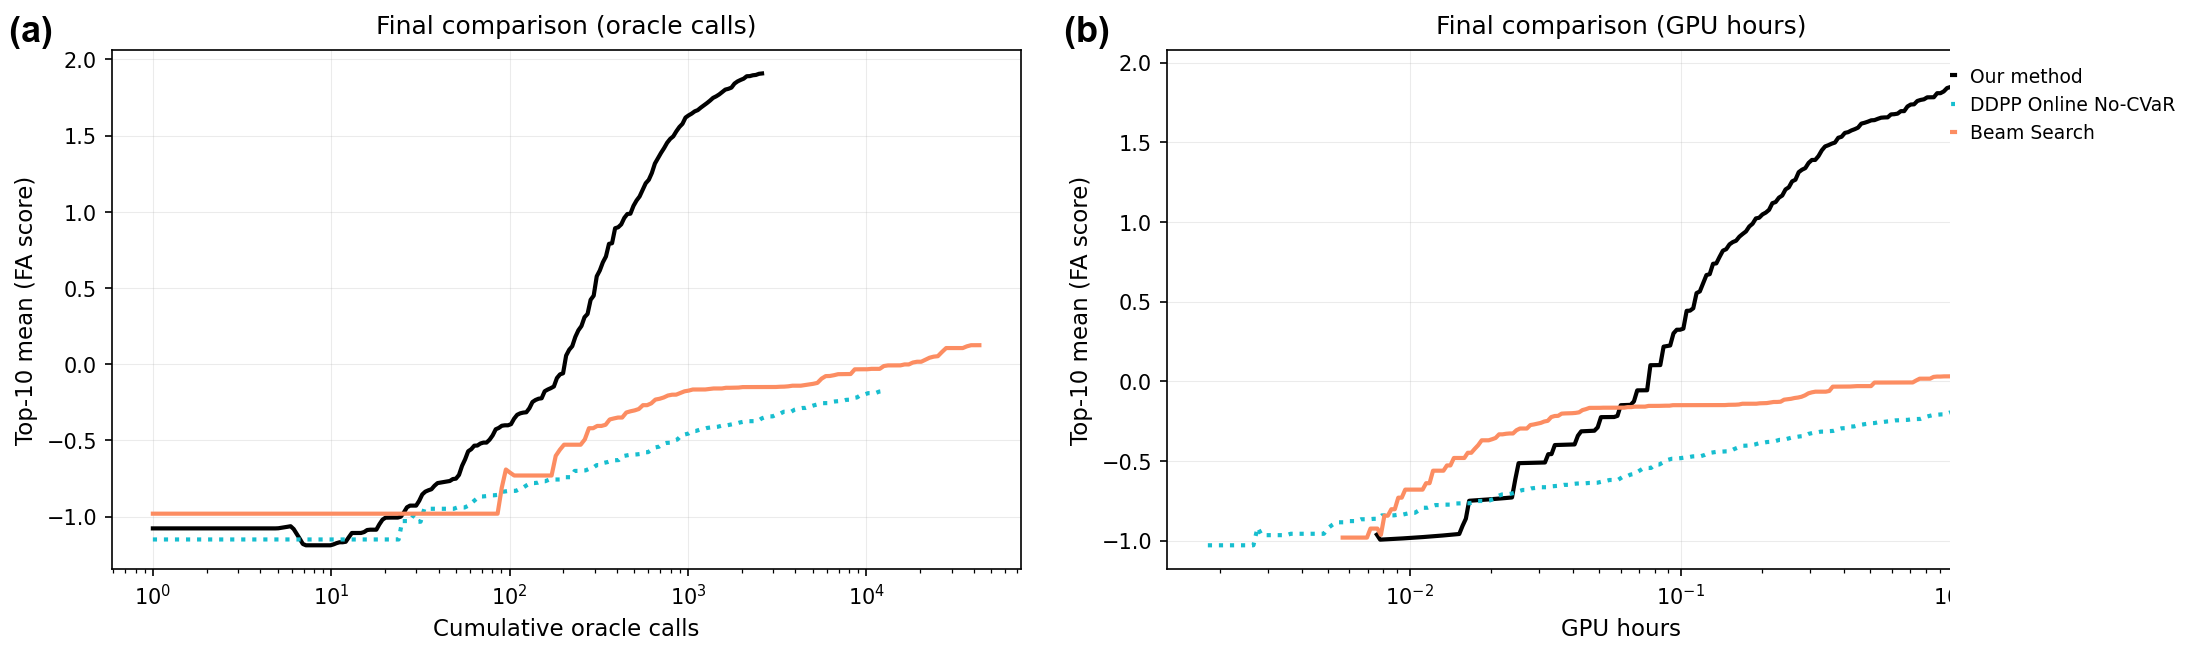
\includegraphics[width=\textwidth]{figures/final_comparison.png}
  \caption{\textbf{Final comparison.} Top-10 mean FA score vs.\ (a) cumulative oracle calls and (b) GPU hours, comparing the full online active loop (Our method: DDPP-LB $+$ CVaR $+$ debiasing $+$ Thompson $+$ buffer $+$ invalid penalty) against the strongest pure-search baseline (Beam Search) and untreated online finetuning (DDPP Online No-CVaR). The full stack dominates both baselines under matched compute on the FA oracle.}
  \label{fig:final_comparison}
\end{figure}

\begin{figure}[H]
  \centering
  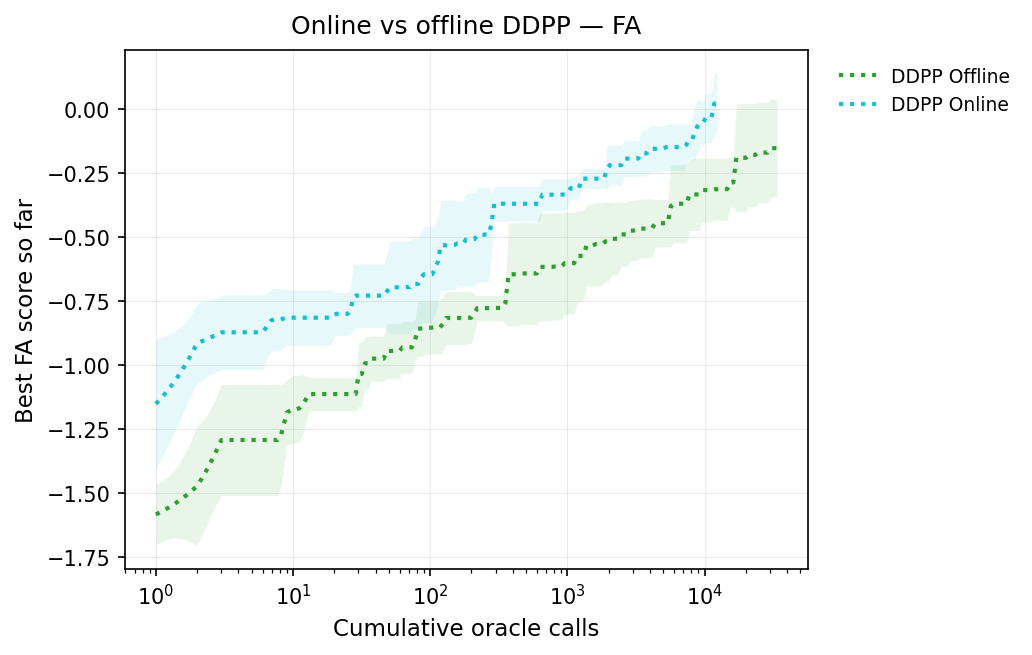
\includegraphics[width=0.49\textwidth]{figures/online_offline_a.png}\hfill
  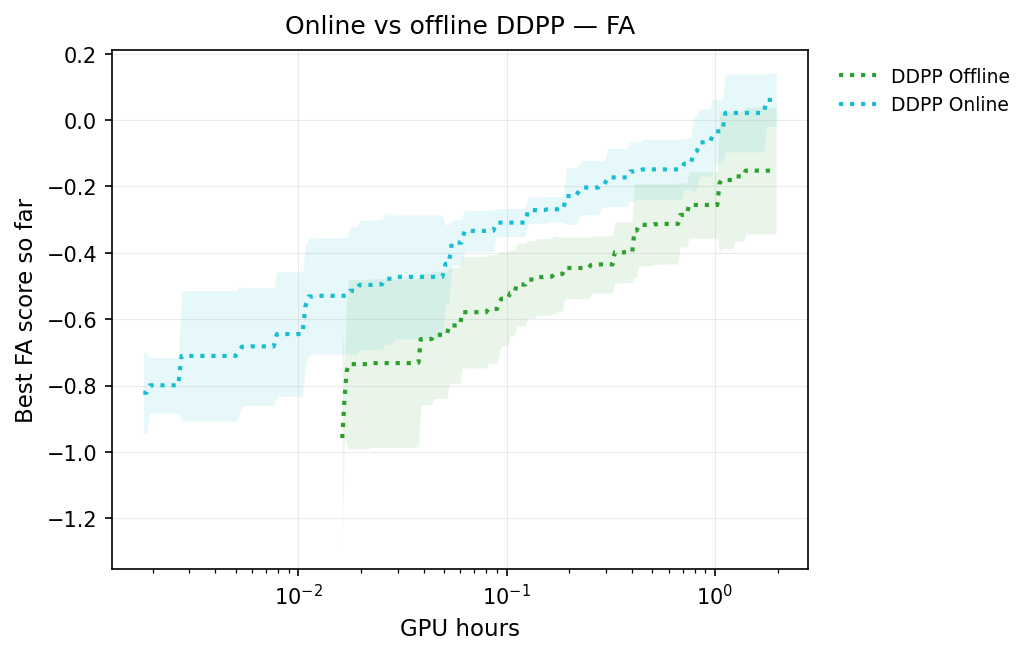
\includegraphics[width=0.49\textwidth]{figures/online_offline_b.png}
  \caption{\textbf{Online vs.\ offline DDPP-LB} on top-1 best FA score so far, against cumulative oracle calls (left) and GPU hours (right). Both runs use the same DDPP-LB loss and no reward shaping; the only difference is whether the buffer of $(x, r(x))$ pairs is collected up front and trained on once (offline) or refreshed continuously by the current $q_\theta$ between gradient steps (online). Seed-averaged ($n{=}5$) bands. Online dominates on both axes: the larger number of gradient updates and the larger volume of policy-correlated data pushed through them push the sampling distribution closer to $p^\star$ than a one-shot offline schedule does.}
  \label{fig:online_vs_offline}
\end{figure}

\subsection{Surrogate screening and Tweedie shortcuts in frozen-generator search}

\begin{figure}[H]
  \centering
  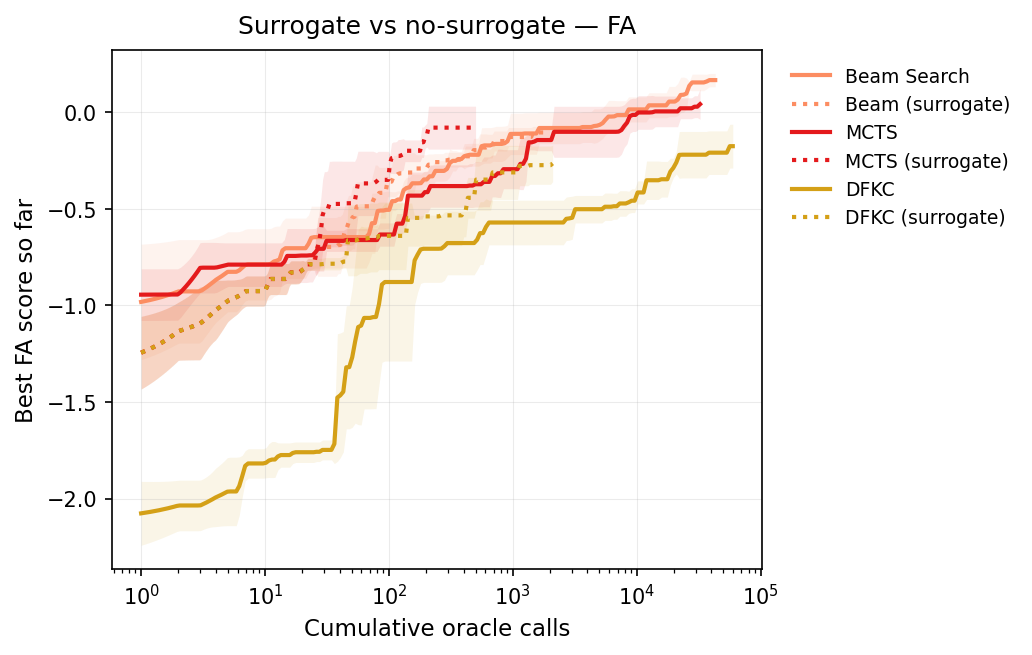
\includegraphics[width=0.49\textwidth]{figures/surrogate_search_a.png}\hfill
  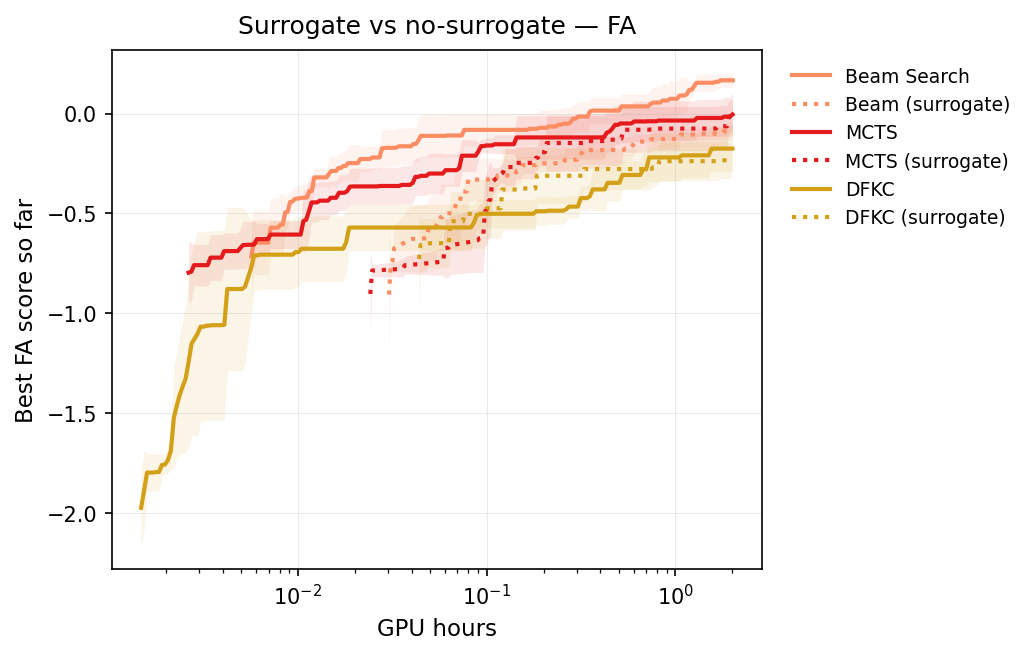
\includegraphics[width=0.49\textwidth]{figures/surrogate_search_b.png}
  \caption{\textbf{Surrogate screening on inference-time search.} Beam, MCTS, and DFKC each compared against their surrogate-pre-filter variant (cheap MLP scores all candidates, oracle only sees the top-$K$). Solid: oracle-on-everything. Dashed: surrogate pre-filter. Seed-averaged ($n{=}5$) top-1 best FA against cumulative oracle calls (left) and GPU hours (right). Surrogate screening dominates plain search on both axes across all three families: each oracle call is spent on a candidate that already cleared the cheap filter, so the per-call yield is higher.}
  \label{fig:surrogate_search}
\end{figure}

\begin{figure}[H]
  \centering
  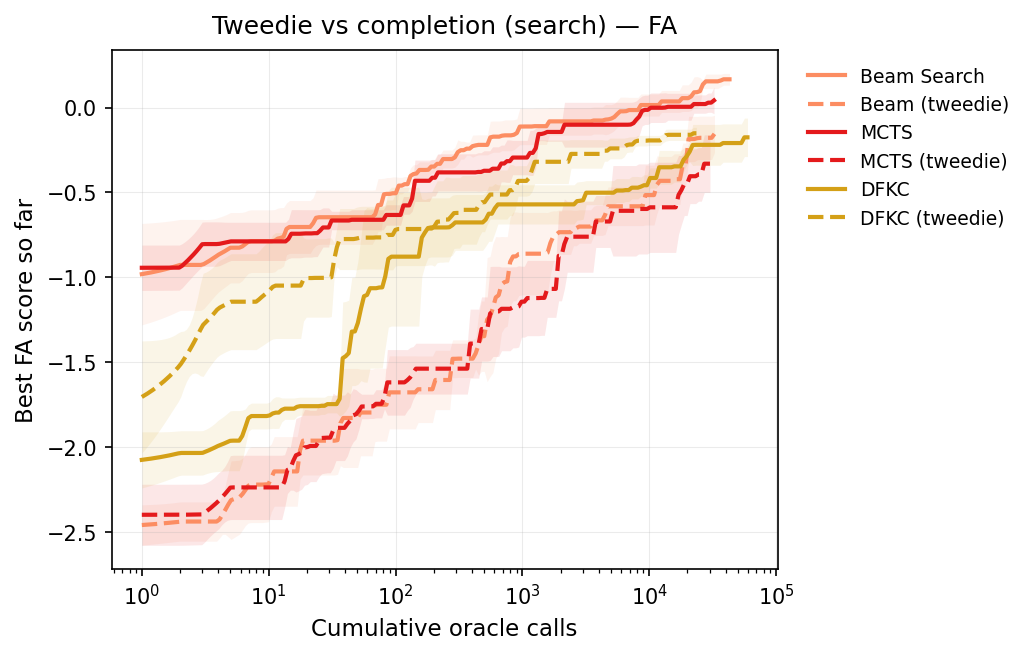
\includegraphics[width=0.49\textwidth]{figures/tweedie_search_a.png}\hfill
  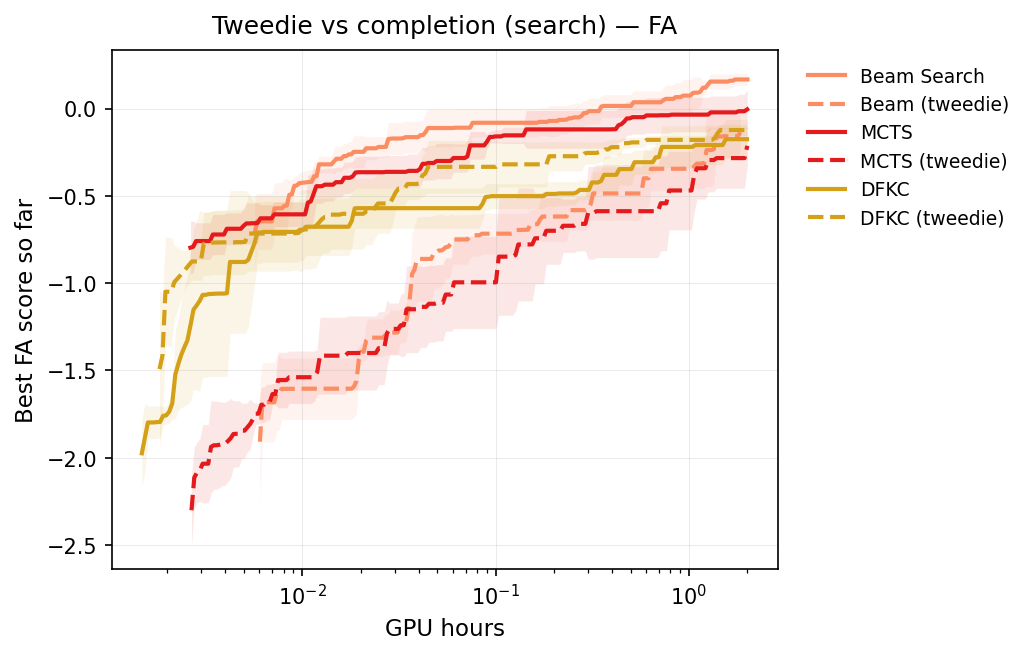
\includegraphics[width=0.49\textwidth]{figures/tweedie_search_b.png}
  \caption{\textbf{Tweedie vs.\ completion (inference-time search).} Same beam/MCTS/DFKC families as above. Solid: completion (full denoising rollout to score). Dashed: Tweedie posterior-mean estimate $\hat{x}_0 = \mathbb{E}[x_0 \mid x_t]$ in place of the rollout. Seed-averaged ($n{=}5$). The Tweedie estimator's noise in the discrete setting is reflected directly in score: every Tweedie variant underperforms its completion counterpart, and the gap is largest for DFKC. The diffusion-pass savings do not translate into top-1 oracle score because the per-step score estimate is too noisy to steer the search.}
  \label{fig:tweedie_search}
\end{figure}

\begin{figure}[H]
  \centering
  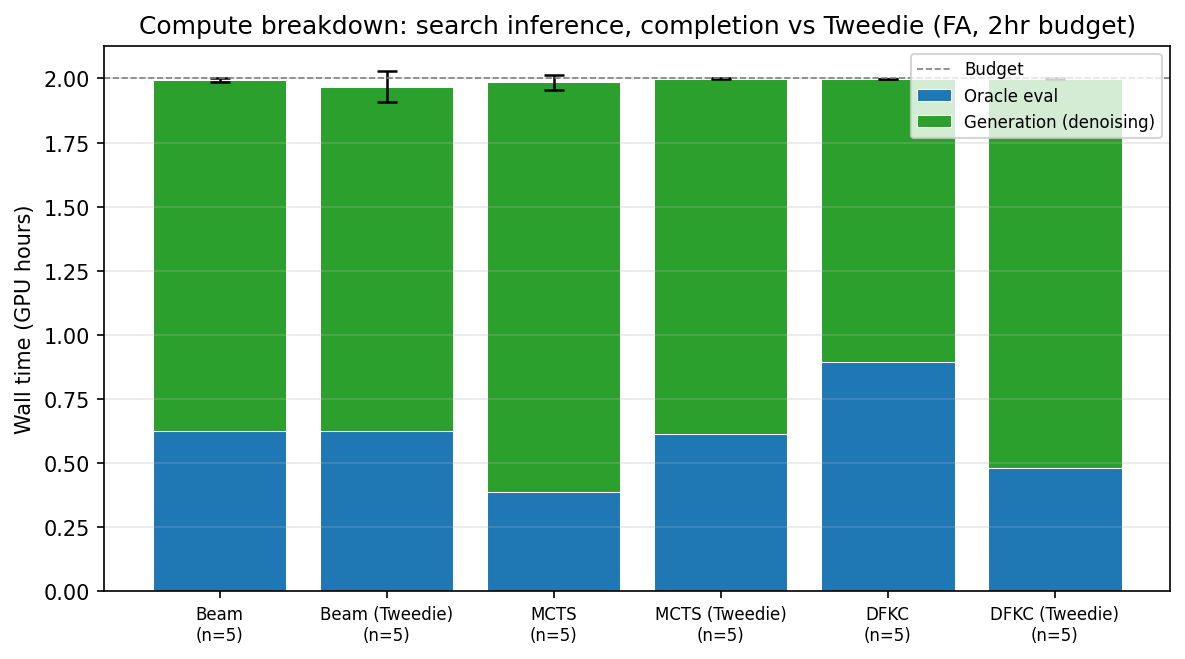
\includegraphics[width=0.85\textwidth]{figures/fig_tweedie_inference_compute.png}
  \caption{\textbf{Compute breakdown for inference-time search, completion vs.\ Tweedie.} Stacked bars are seed-averaged ($n{=}5$) wall-clock spend at the $2$-hour FA budget; oracle compute is estimated as $n_{\text{calls}} \times c_{\text{FA}}$ with $c_{\text{FA}} \approx 50$\,ms (matched to the per-phase log on the active runs). Tweedie shifts the per-family balance but does not recover enough wall time to compensate for the score loss in Fig.~\ref{fig:tweedie_search}: for MCTS it produces more oracle calls in the same budget, for DFKC it produces fewer. Generation dominates total wall time in every cell.}
  \label{fig:tweedie_inference_compute}
\end{figure}

\subsection{Search inside the online adaptation loop}

\begin{figure}[H]
  \centering
  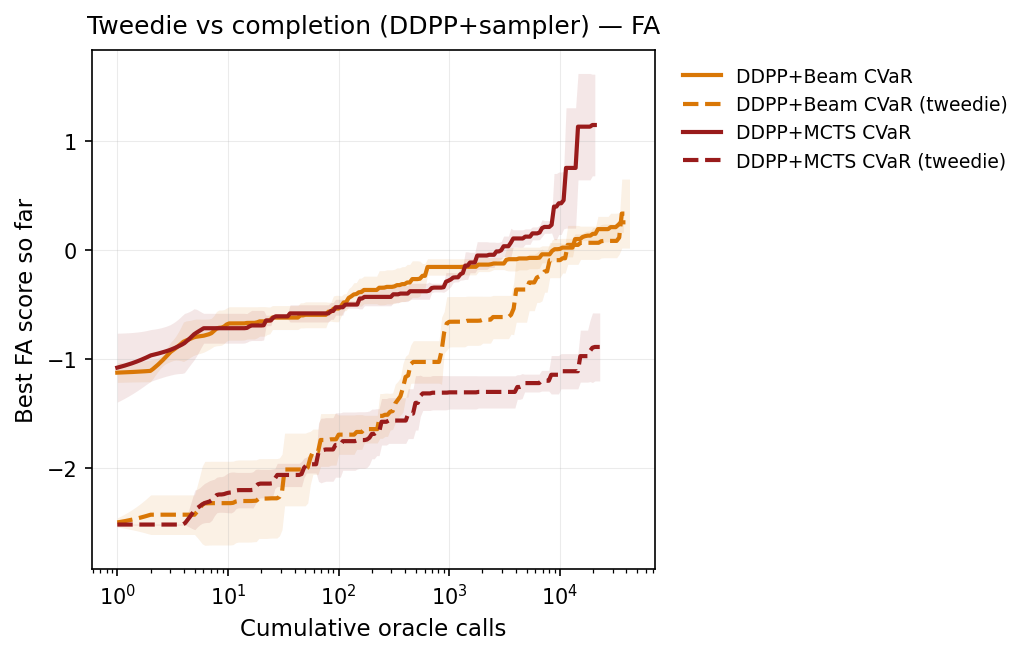
\includegraphics[width=0.49\textwidth]{figures/tweedie_active_a.png}\hfill
  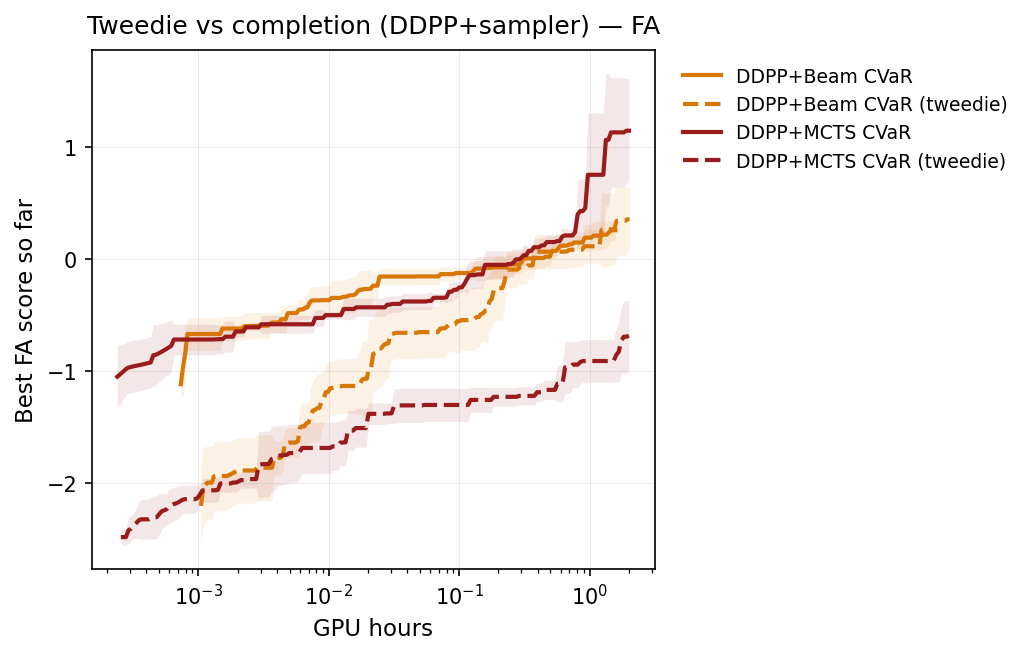
\includegraphics[width=0.49\textwidth]{figures/tweedie_active_b.png}
  \caption{\textbf{Tweedie vs.\ completion (active hybrids).} Same Tweedie/completion comparison but applied inside the online DDPP-LB hybrids of Sec.~\ref{sec:results} (beam and MCTS only; DFKC is not paired here). Solid: completion. Dashed: Tweedie. Seed-averaged ($n{=}5$). The Tweedie variants underperform their completion counterparts here as well, despite the saved generation passes nominally freeing time for fine-tuning.}
  \label{fig:tweedie_active}
\end{figure}

\begin{figure}[H]
  \centering
    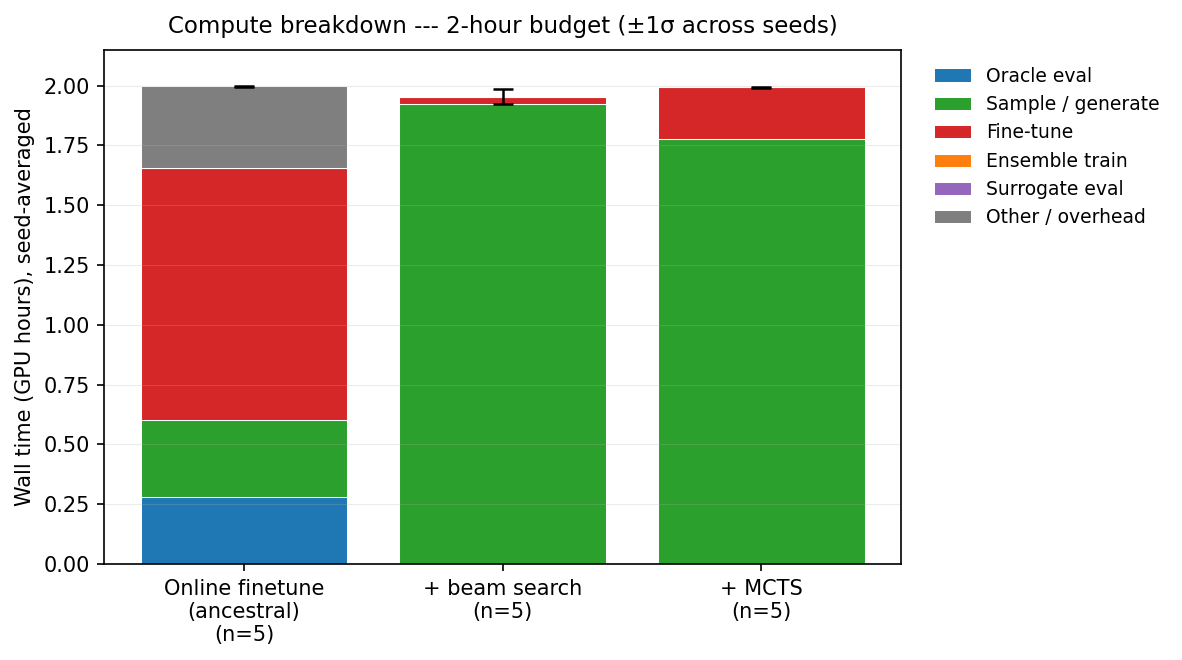
\includegraphics[width=0.85\textwidth]{figures/fig_search_overhead.png}
  \caption{Compute breakdown under a 2-hour wall budget for plain online finetuning (left) versus online finetuning augmented with beam search (middle) or MCTS (right). All numbers are seed-averaged ($n{=}5$). Plain online finetune spends roughly half its budget on fine-tuning ($\sim$1.0\,hr); both search variants spend almost the entire budget on candidate generation, leaving nearly no time for fine-tuning gradient steps ($\sim$0.04\,hr for beam, $\sim$0.21\,hr for MCTS). The reduction in fine-tuning wall time is the proximate reason search-augmented online finetuning fails to improve over the plain variant.}
  \label{fig:search_overhead}
\end{figure}

\begin{figure}[H]
  \centering
  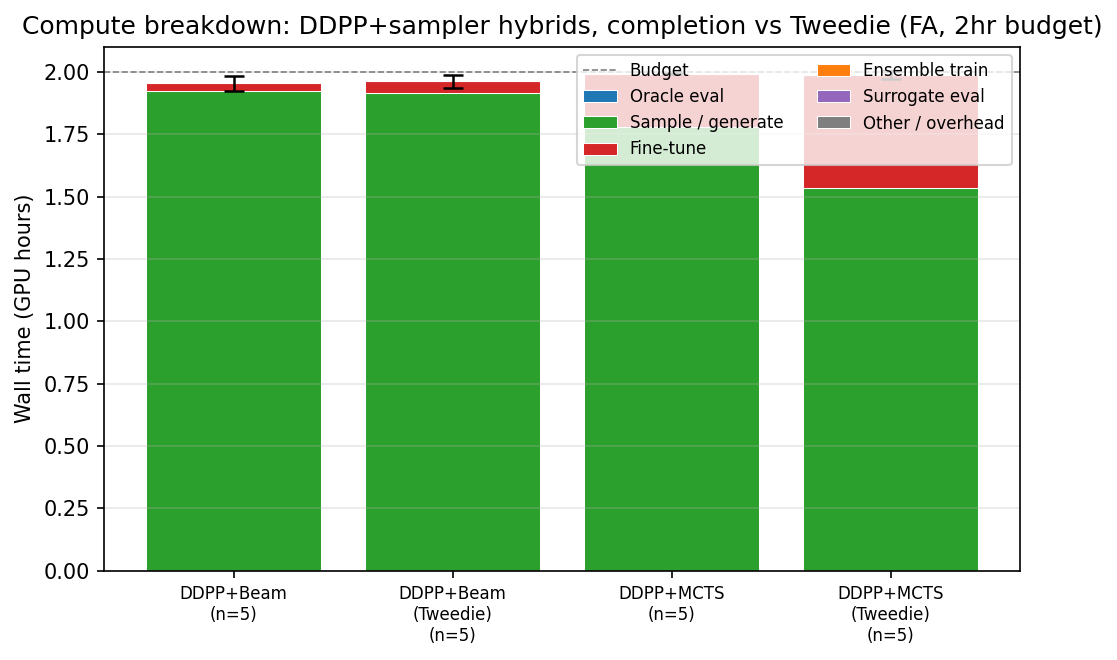
\includegraphics[width=0.85\textwidth]{figures/fig_tweedie_active_compute.png}
  \caption{\textbf{Compute breakdown for active hybrids, completion vs.\ Tweedie.} Per-phase wall times pulled from \texttt{active\_loop\_log.jsonl}; seed-averaged ($n{=}5$). Generation dominates for both completion and Tweedie variants, leaving very little wall time for fine-tuning ($\leq 0.1$\,hr) regardless of whether the search uses the Tweedie shortcut or completion. The fine-tuning budget reduction observed for completion-based hybrids in Fig.~\ref{fig:search_overhead} is not relieved by the Tweedie shortcut.}
  \label{fig:tweedie_active_compute}
\end{figure}

\subsection{Compute accounting and oracle-cost sensitivity}

To pull apart why test-time finetuning beats inference-time search, it helps to look at where each method actually spends its wall-clock budget. We log per-call elapsed time alongside the oracle score in every run (Sec.~\ref{sec:exp-setup}), which lets us decompose each method's wall time into the components of Eq.~\ref{eq:wall-decomp}: oracle evaluation ($N \cdot c_{\text{oracle}}$), candidate generation, fine-tuning gradient steps, surrogate ensemble training, and bookkeeping. The same per-call timeline supports a retroactive cost analysis: scaling the per-call oracle cost $c_{\text{oracle}}$ by $100\times$ simulates a switch from a fast oracle (FA) to a slow oracle (Boltz-2-class) without re-running anything. Appendix Fig.~\ref{fig:compute_breakdown} shows the resulting breakdowns side-by-side.

The takeaway is that finetuning's advantage over search comes mostly from not spending the budget on oracle calls. Each gradient step extracts more usable signal per oracle call than a one-shot search evaluation does, so the same oracle budget does more work. The advantage widens further as the oracle gets more expensive: the $100\times$ panel is closer to where Boltz-2-class oracles actually live, and there the full-loop compute breakdown is dominated by generation and surrogate training rather than oracle evaluation.

\begin{figure}[H]
  \centering
  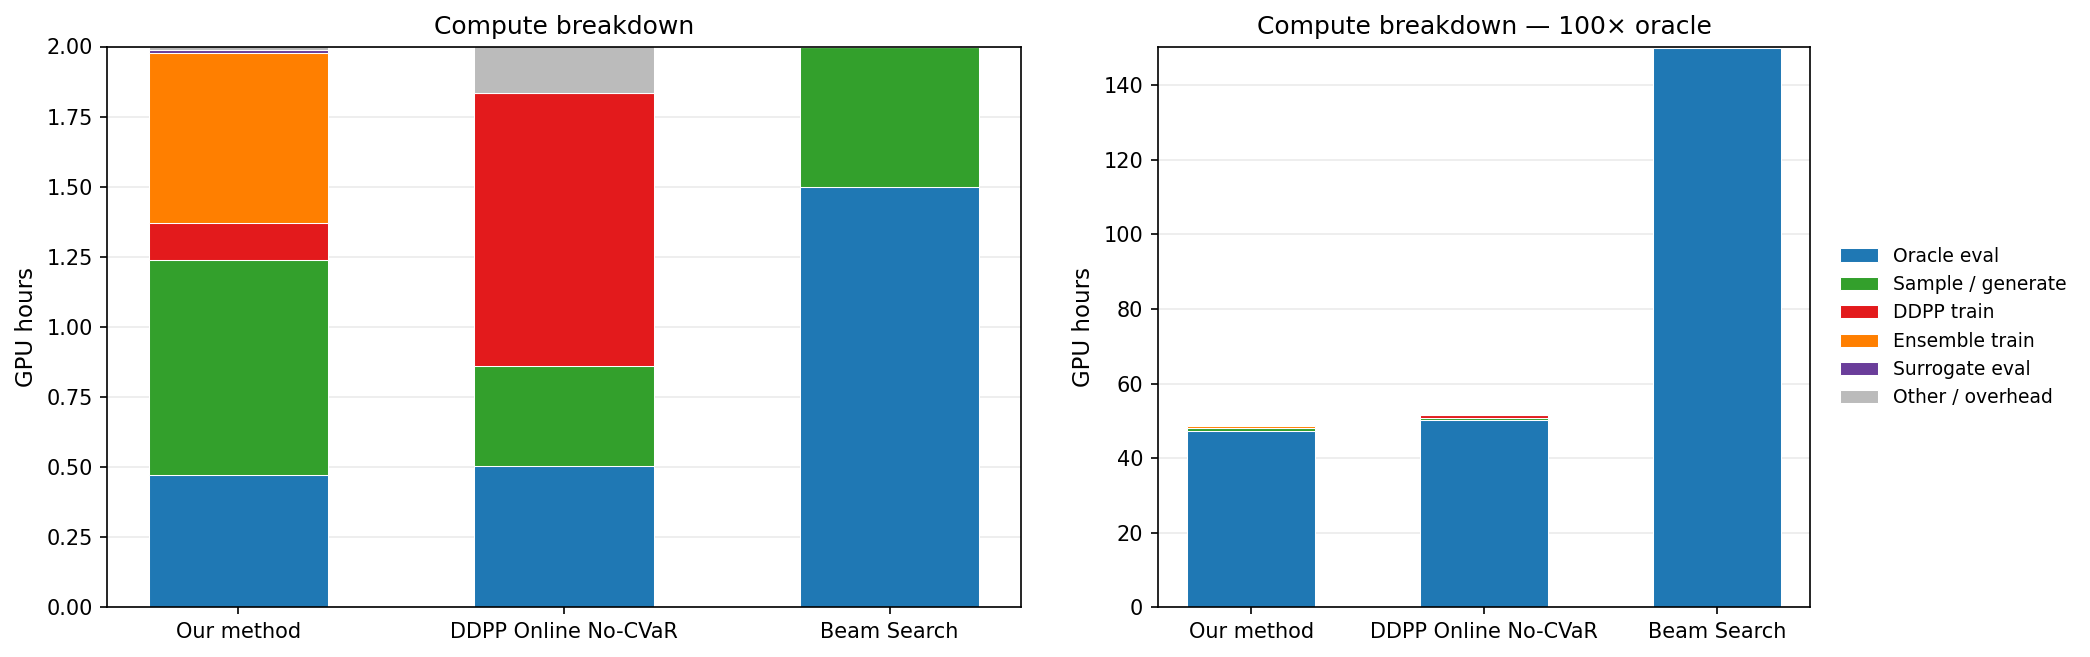
\includegraphics[width=\textwidth]{figures/fig9_ab.png}
  \caption{\textbf{Compute breakdown.} Per-method decomposition of wall-clock spend at standard FA oracle cost (left, $1\times$) and under a retroactive $100\times$ oracle-cost rescaling (right). Pure search spends almost all of its budget on oracle calls, so its absolute compute scales nearly linearly with $c_{\text{oracle}}$. Online finetuning amortizes generation and gradient updates across the same oracle budget, so its share of oracle compute is smaller and the absolute compute under the $100\times$ rescaling grows much less.}
  \label{fig:compute_breakdown}
\end{figure}

\begin{figure}[H]
  \centering
  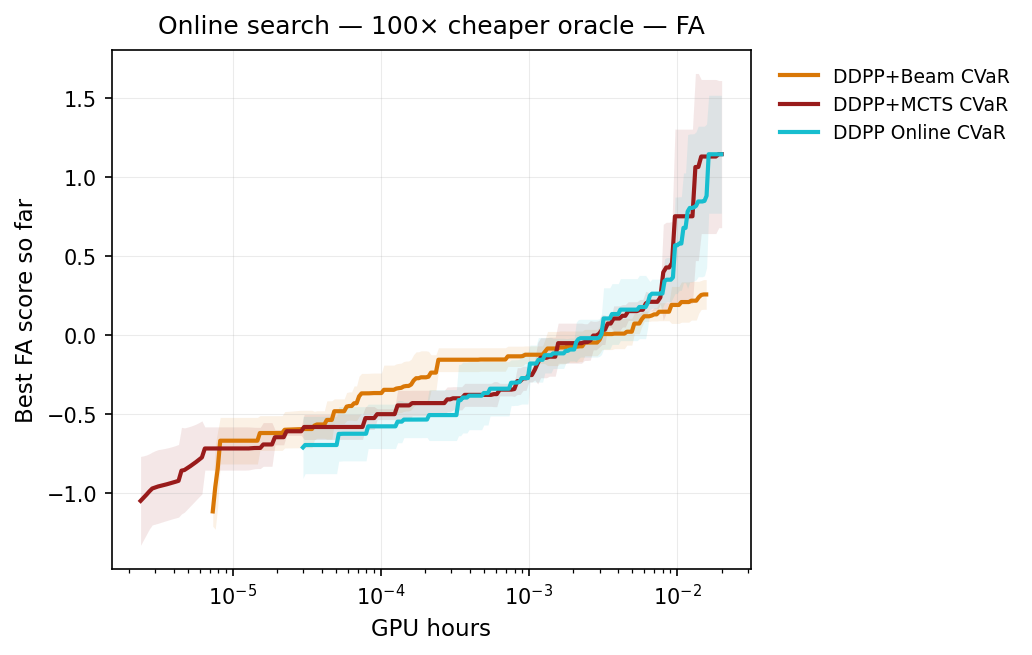
\includegraphics[width=0.49\textwidth]{figures/oracle_rescale_cheaper.png}\hfill
  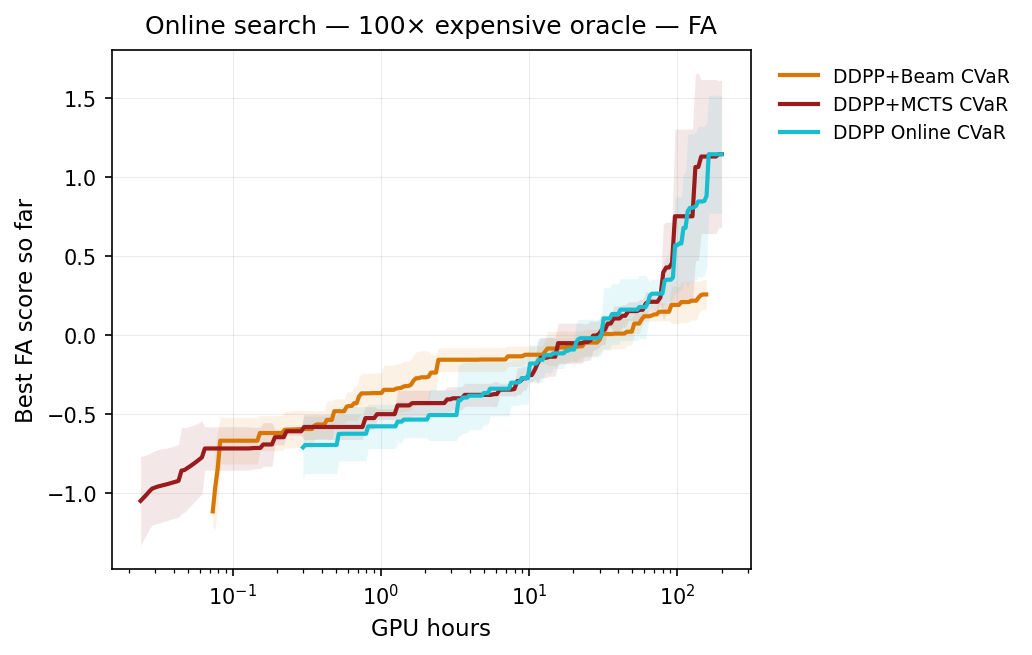
\includegraphics[width=0.49\textwidth]{figures/oracle_rescale_expensive.png}
  \caption{\textbf{Retroactive oracle-cost rescaling on online search hybrids.} Same three online methods (\texttt{ddpp\_online\_cvar} vs.\ \texttt{ddpp\_beam\_cvar} vs.\ \texttt{ddpp\_mcts\_cvar}) plotted on the GPU-hours axis with the per-call oracle cost rescaled by $1/100$ (left) and by $100$ (right). Rescaling shifts the GPU-hours axis by four orders of magnitude in either direction without altering the relative ordering: plain online DDPP-LB matches or exceeds both search-augmented variants under both regimes, supporting the claim in Sec.~\ref{sec:results} that the marginal value of inference-time search on top of online finetuning is robust to oracle expense.}
  \label{fig:oracle_rescale}
\end{figure}

\clearpage

\section{Task-Level and Aggregate Results}\label{app:results-detail}

This section first preserves target-specific variation and then aggregates the same comparisons across domains and compute axes.

% Previous heading: \section{Per-task side-by-side ablation grids}\label{app:per-task-ablation}
\subsection{Per-Task Side-by-Side Ablation Grids}\label{app:per-task-ablation}

The main-text figures (Fig.~\ref{fig:ablation_ddpp}, Fig.~\ref{fig:ablation_search}, and Fig.~\ref{fig:ablation_vidd} in Appendix~\ref{app:vidd-ablation}) hold the finetuner / search-family fixed and step through the $9$ tasks. The figures below transpose that view: each $3 \times 3$ grid groups rows by task and places DDPP-LB, VIDD, and search-only baselines side by side per task. Same normalised-reward definition and conventions as Sec.~\ref{sec:exp-setup}.

\begin{figure}[H]
  \centering
  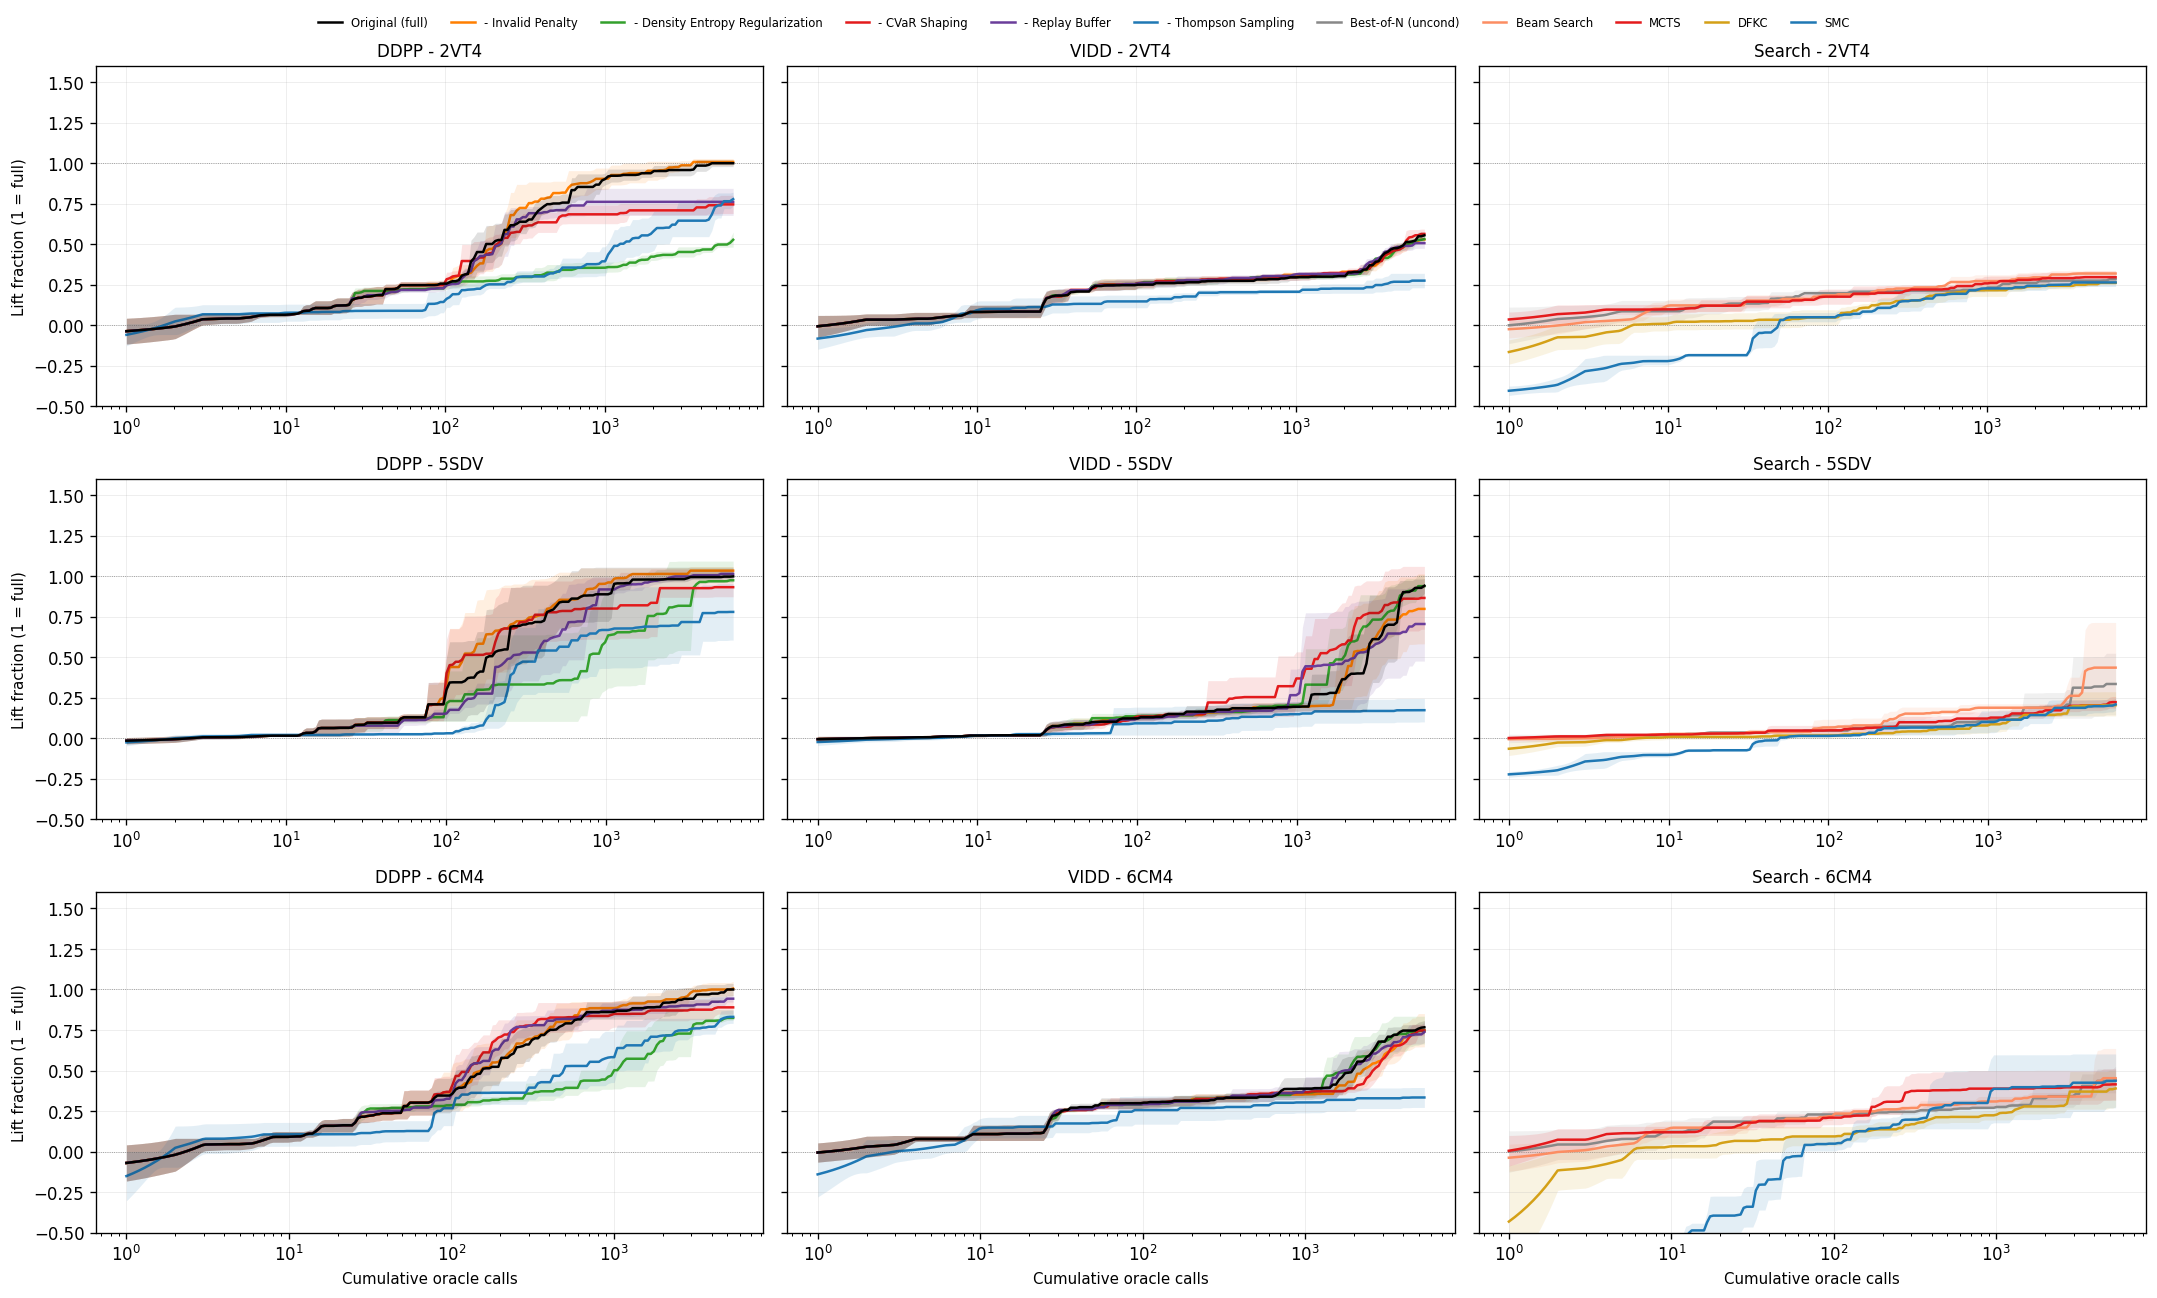
\includegraphics[width=0.95\textwidth]{figures/ablations/mol_ablations_grid_set1_norm.png}
  \caption{\textbf{Per-task ablation, small molecules (set 1: 2VT4, 5SDV, 6CM4).} Rows are FA-oracle targets; columns are DDPP-LB ablations (left), VIDD ablations (centre), search baselines (right). The VIDD column is consistently more compressed than DDPP-LB on the same target, matching the cross-finetuner observation in Fig.~\ref{fig:ablation_vidd}.}
  \label{fig:per_task_mol_set1}
\end{figure}

\begin{figure}[H]
  \centering
  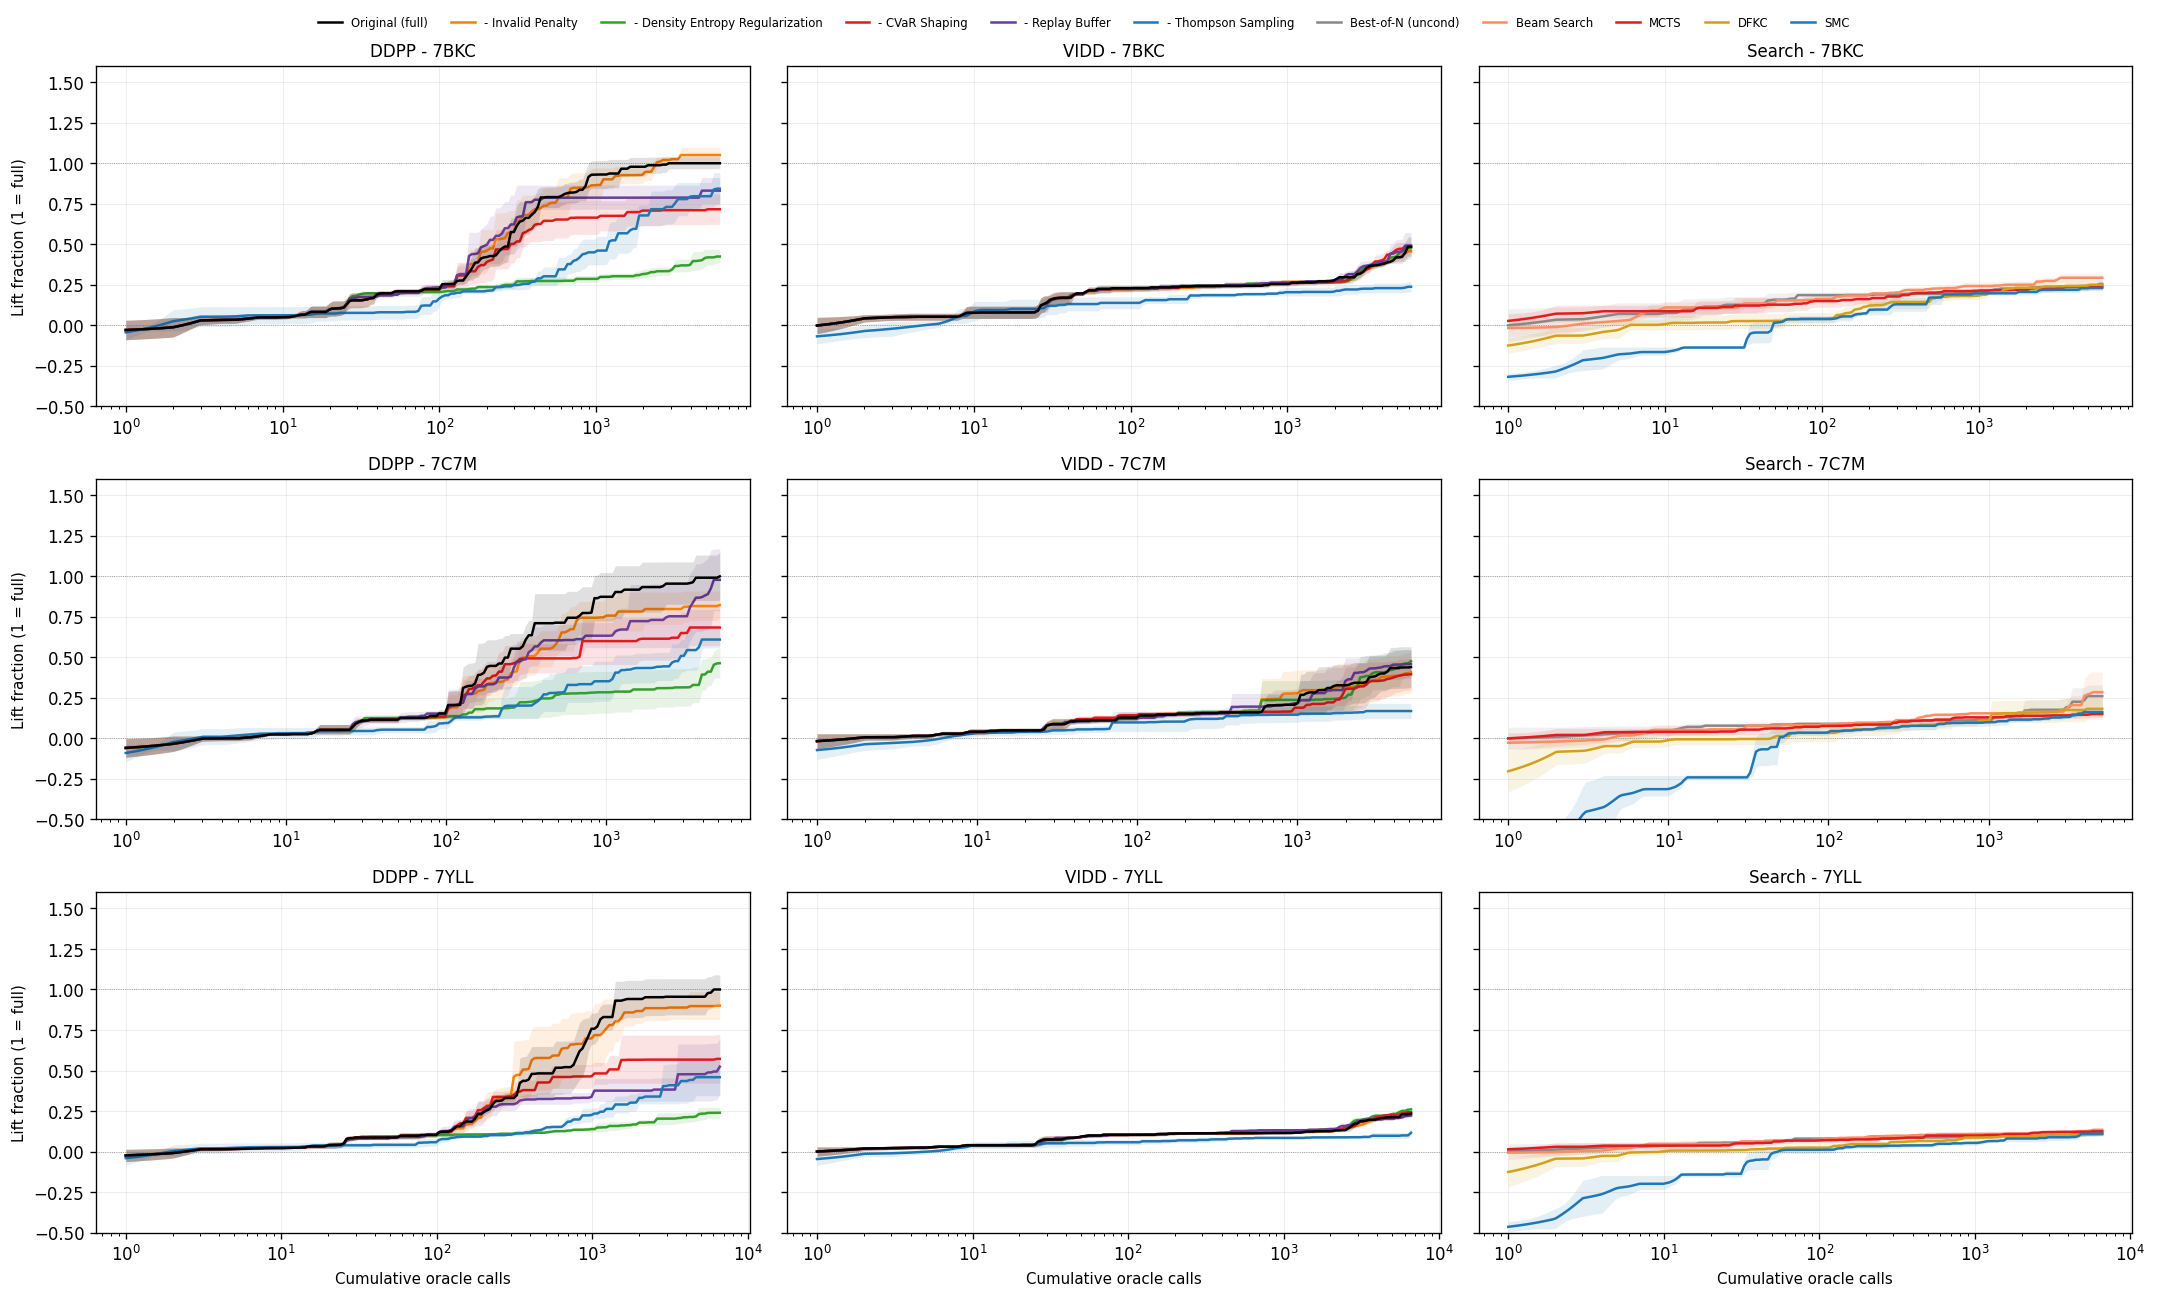
\includegraphics[width=0.95\textwidth]{figures/ablations/mol_ablations_grid_set2_norm.png}
  \caption{\textbf{Per-task ablation, small molecules (set 2: 7BKC, 7C7M, 7YLL).} Continuation of Fig.~\ref{fig:per_task_mol_set1} for the remaining three FA-oracle targets. The 7C7M row is extreme: removing \textit{- density entropy regularization} drops DDPP-LB to a small fraction of the full method, while the same removal under VIDD has a much smaller effect --- consistent with the student-teacher damping of policy drift discussed in Appendix~\ref{app:vidd-ablation}.}
  \label{fig:per_task_mol_set2}
\end{figure}

\begin{figure}[H]
  \centering
  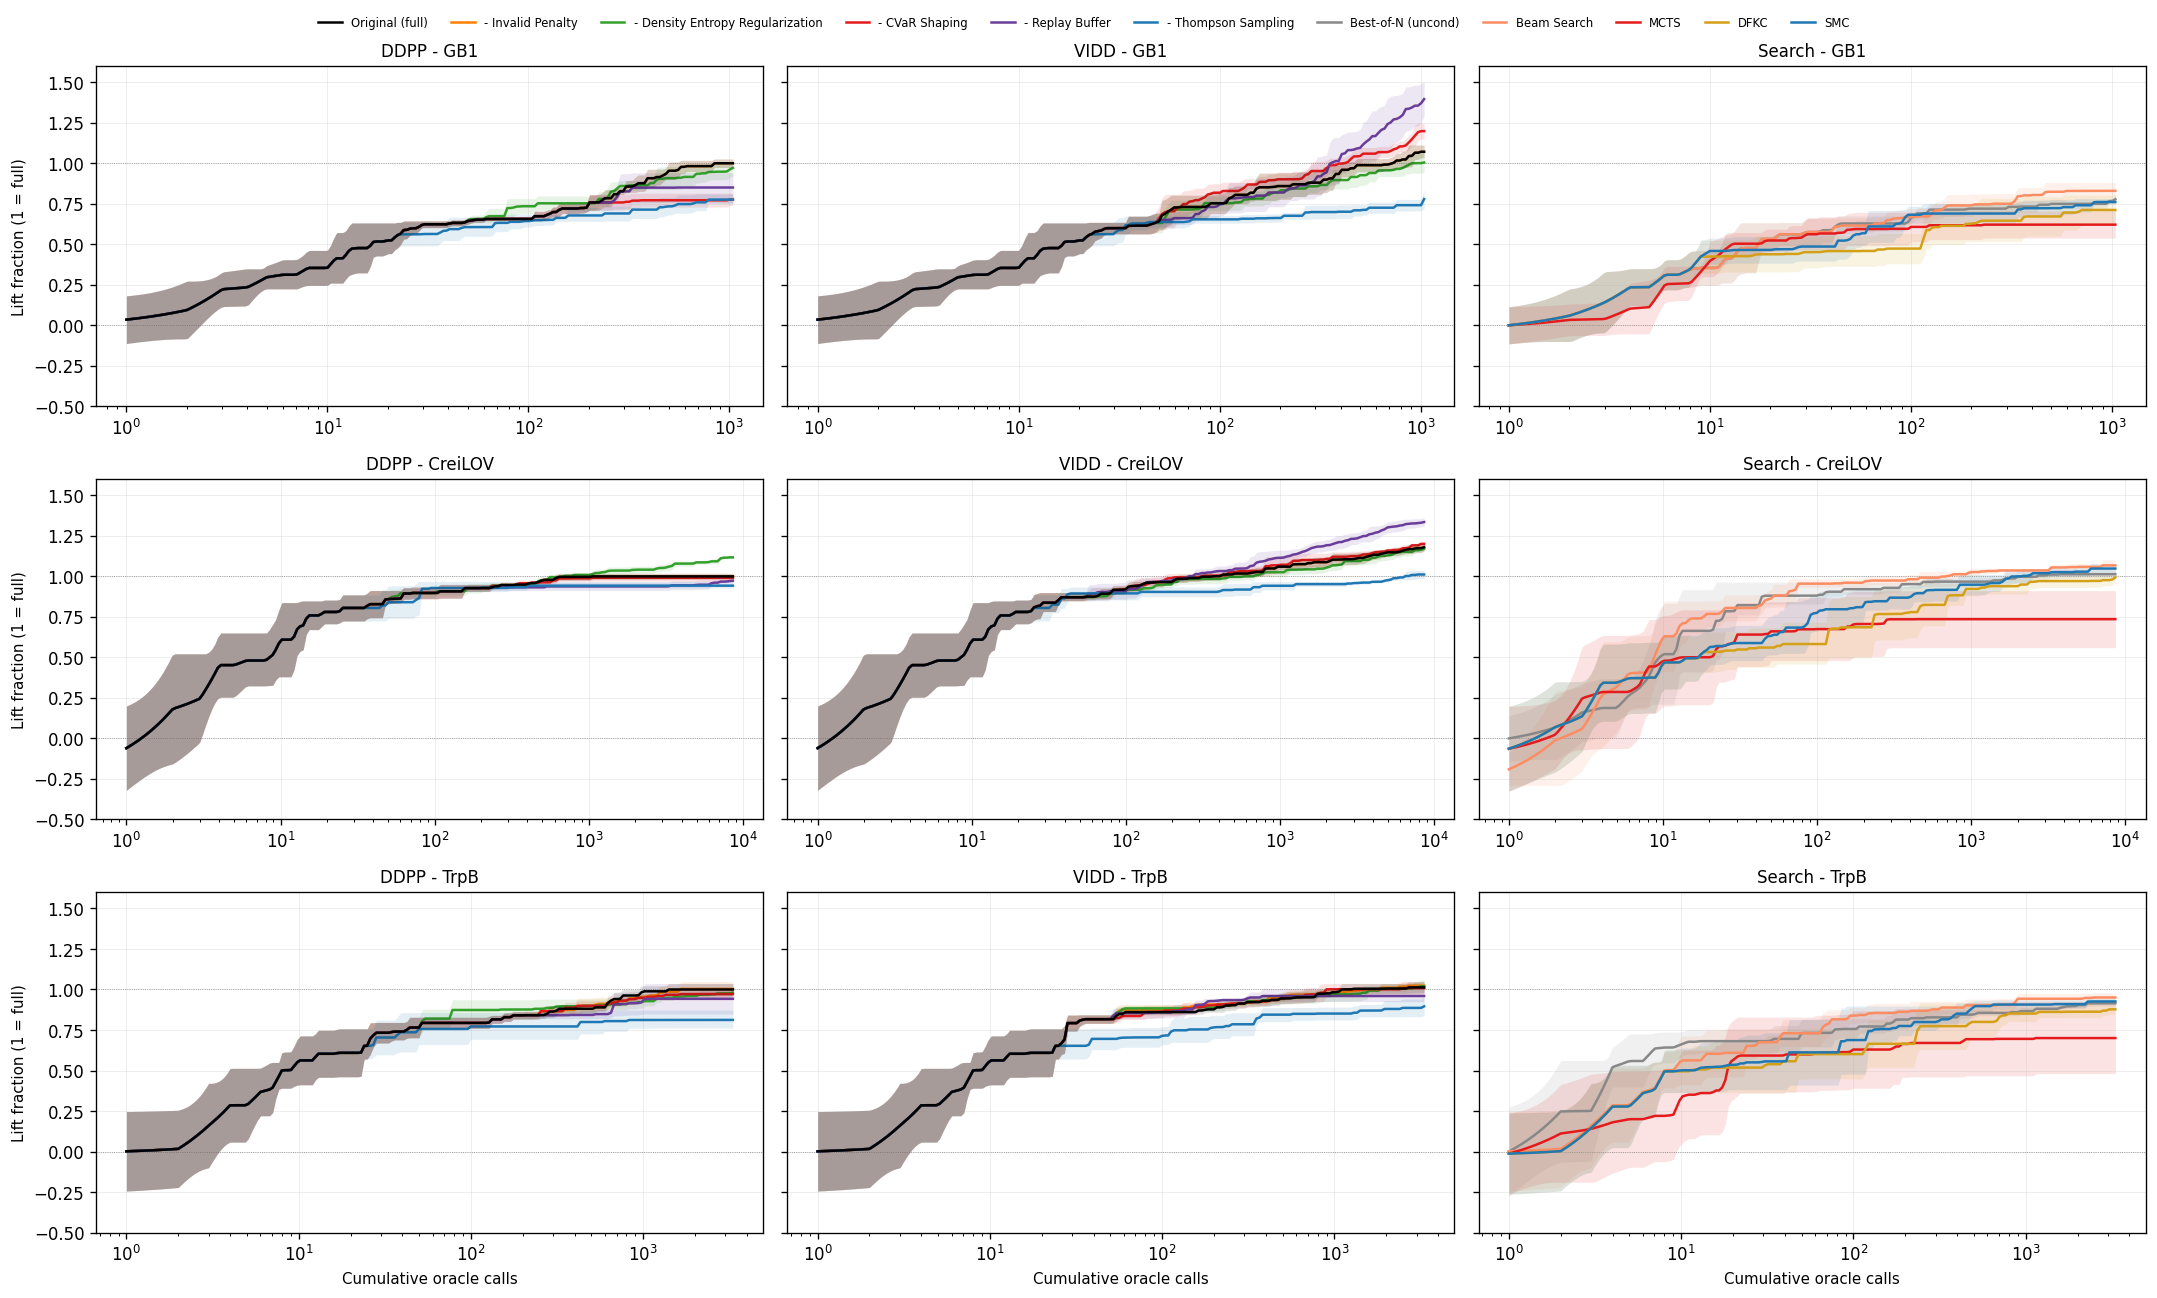
\includegraphics[width=0.95\textwidth]{figures/ablations/protein_ablations_grid_norm.png}
  \caption{\textbf{Per-task ablation, protein-fitness targets (GB1, CreiLOV, TrpB).} Rows are protein-fitness families; columns match Fig.~\ref{fig:per_task_mol_set1}. CI bands are wider than the small-molecule rows because each family has a single trained surrogate / generator pair (no within-family pooling).}
  \label{fig:per_task_protein}
\end{figure}

\begin{figure}[H]
  \centering
  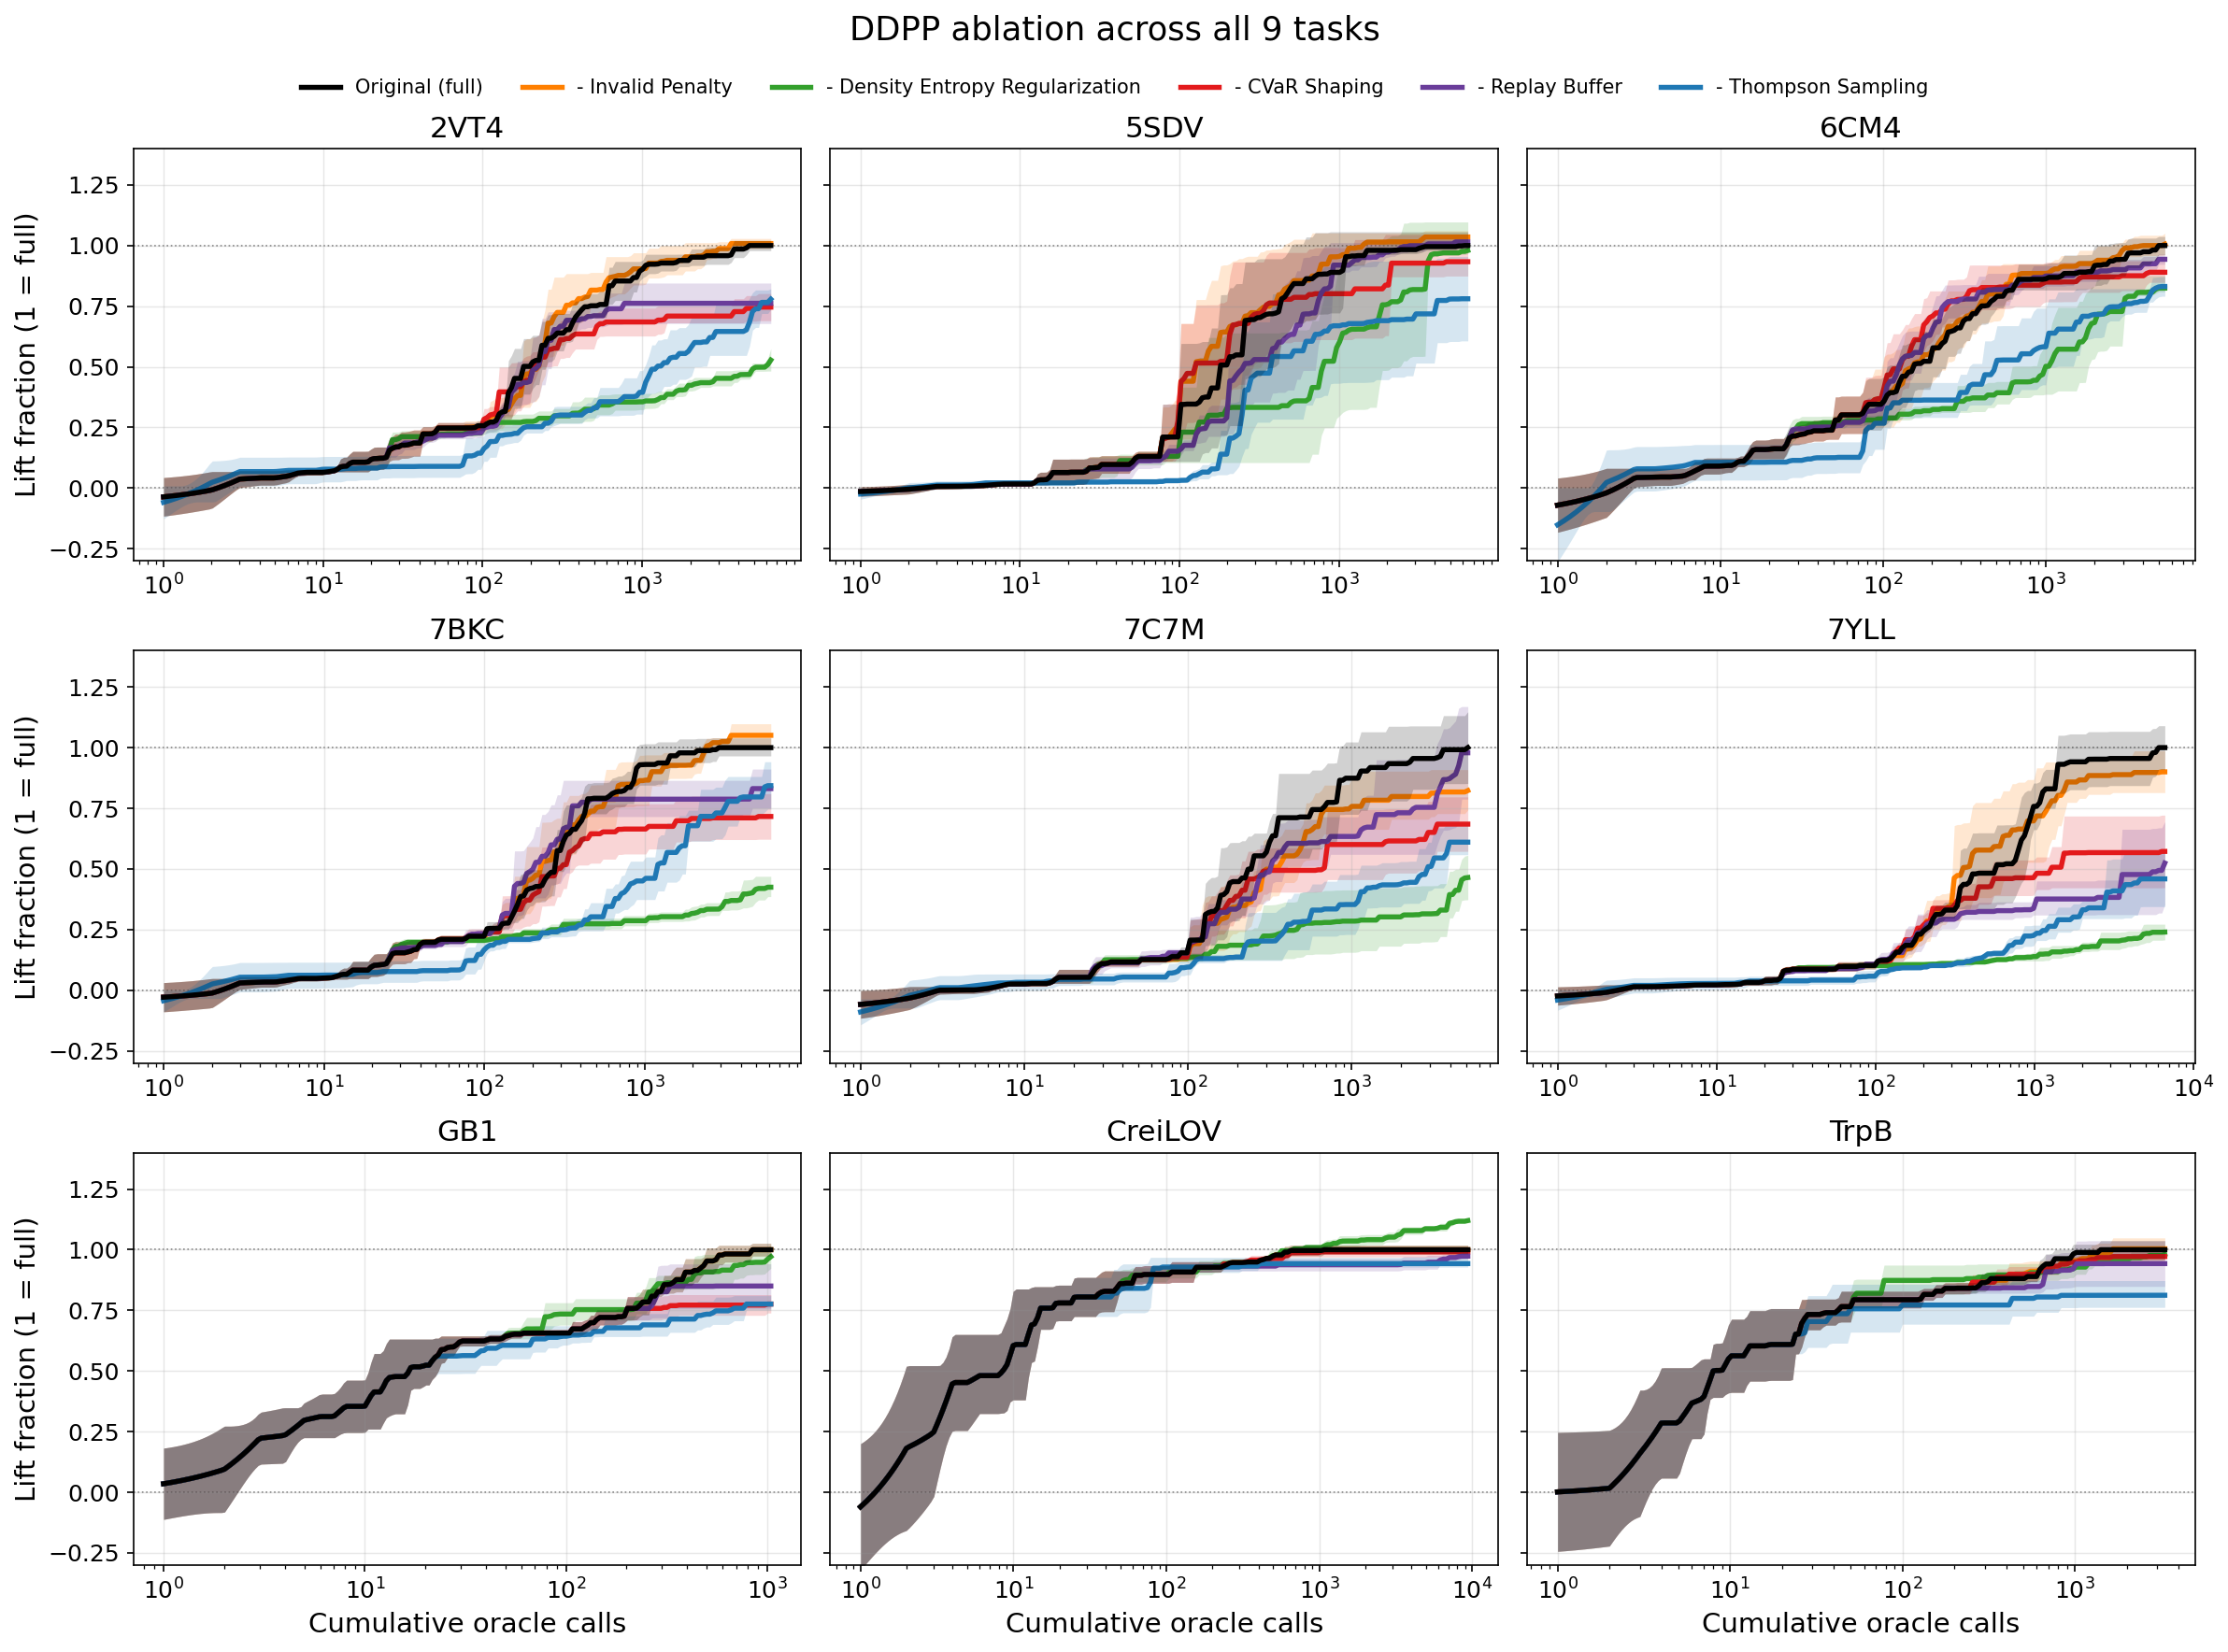
\includegraphics[width=\textwidth]{figures/ablations/ddpp_only_grid_norm.png}
  \caption{\textbf{DDPP-LB harness ablation across all $9$ tasks.} Normalised reward $(1 =$ full DDPP-LB on that target$)$ for each leave-one-out ablation of the knobs in Table~\ref{tab:methods}; six FA-oracle small molecules (top two rows) and three protein-fitness families (bottom row). Seeds, CI bands, and budget cap follow Sec.~\ref{sec:exp-setup}. Each knob's contribution varies across tasks, but knob ordering is broadly preserved across targets. VIDD twin: Appendix~\ref{app:vidd-ablation}. Per-task side-by-side: Appendix~\ref{app:per-task-ablation}.}
  \label{fig:ablation_ddpp}
\end{figure}

\begin{figure}[H]
  \centering
  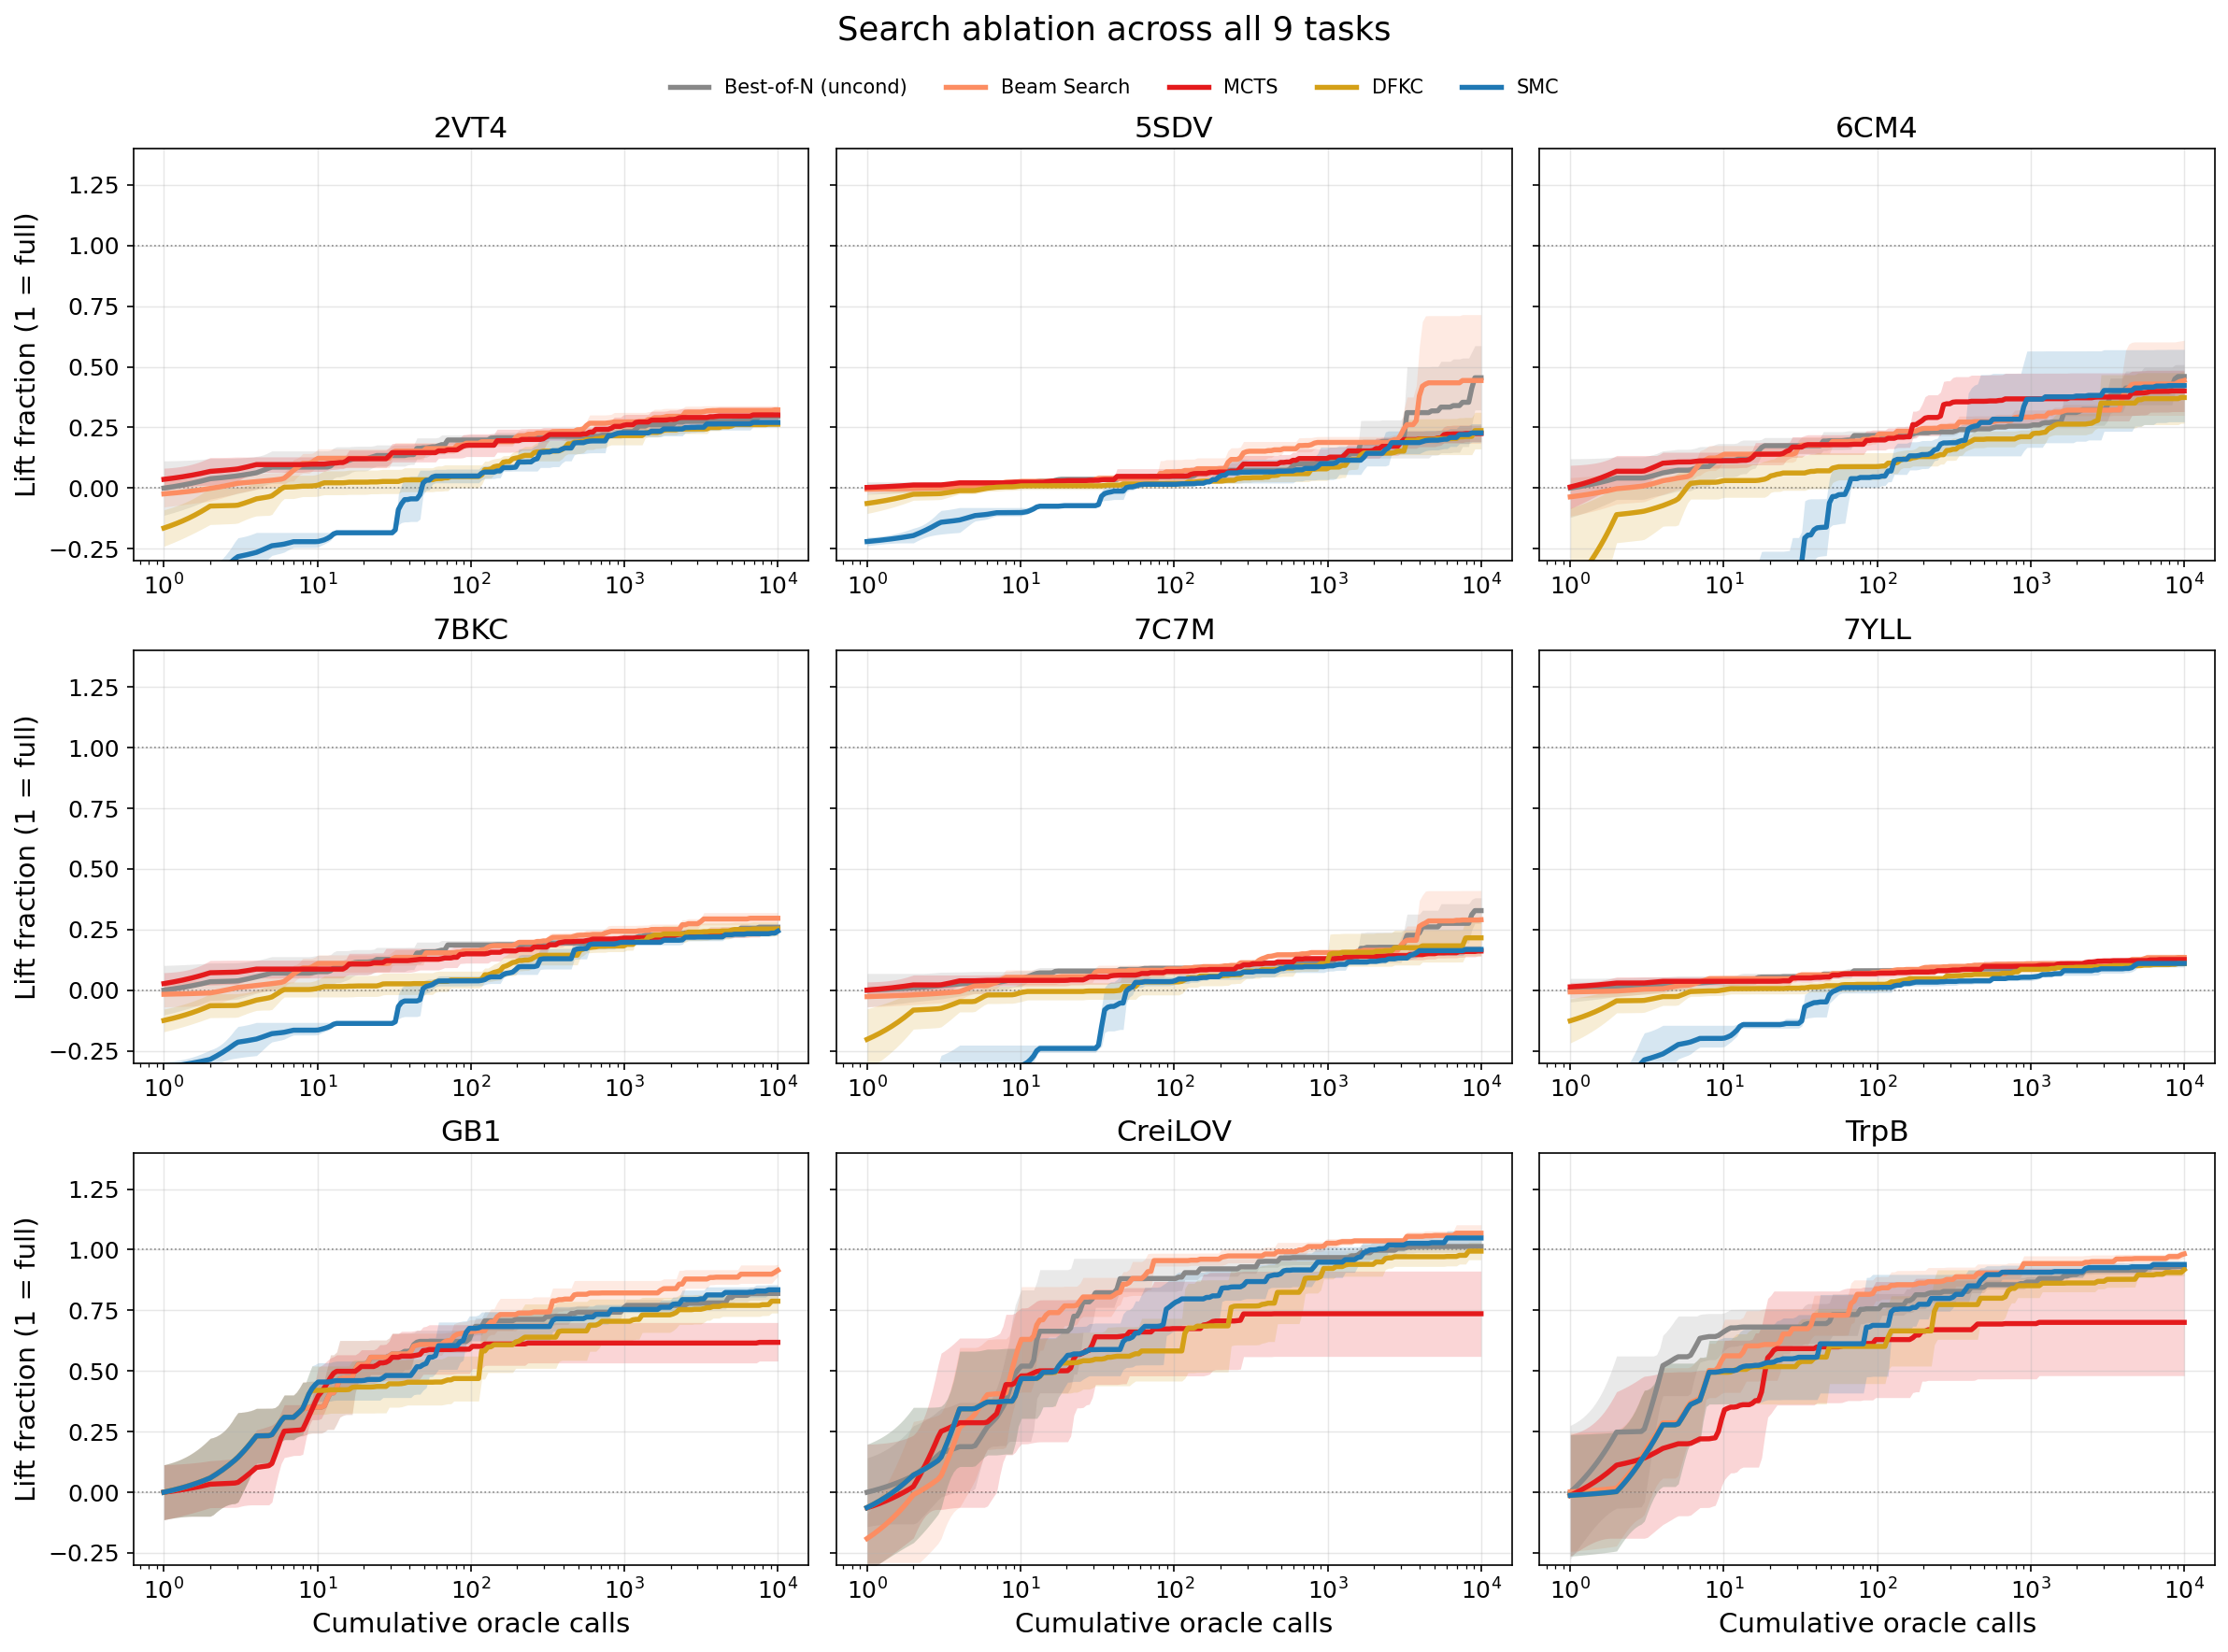
\includegraphics[width=\textwidth]{figures/ablations/search_only_grid_norm.png}
  \caption{\textbf{Inference-time search-only baselines across all $9$ tasks.}} Same normalised-reward definition as Fig.~\ref{fig:ablation_ddpp} applied to the search-only methods (best-of-$N$, beam, MCTS, DFKC, SMC) at matched cumulative-oracle budget.
  \label{fig:ablation_search}
\end{figure}

% Previous heading: \section{Aggregated ablation grids}\label{app:avg-ablation}
\subsection{Aggregated Ablation Grids}\label{app:avg-ablation}

The per-task figures above retain the cross-target spread that motivates the manifold / mode-density discussion in Sec.~\ref{sec:results}. The figures below collapse that spread by averaging the normalised-reward curves across the $6$ FA-oracle small molecules (top row) and across the $3$ protein-fitness families (bottom row), giving a single curve per knob per axis-type. CI bands are across-target ($\pm 1.96 \cdot \mathrm{SEM}$), so they reflect target-level rather than seed-level variability.

\begin{figure}[H]
  \centering
  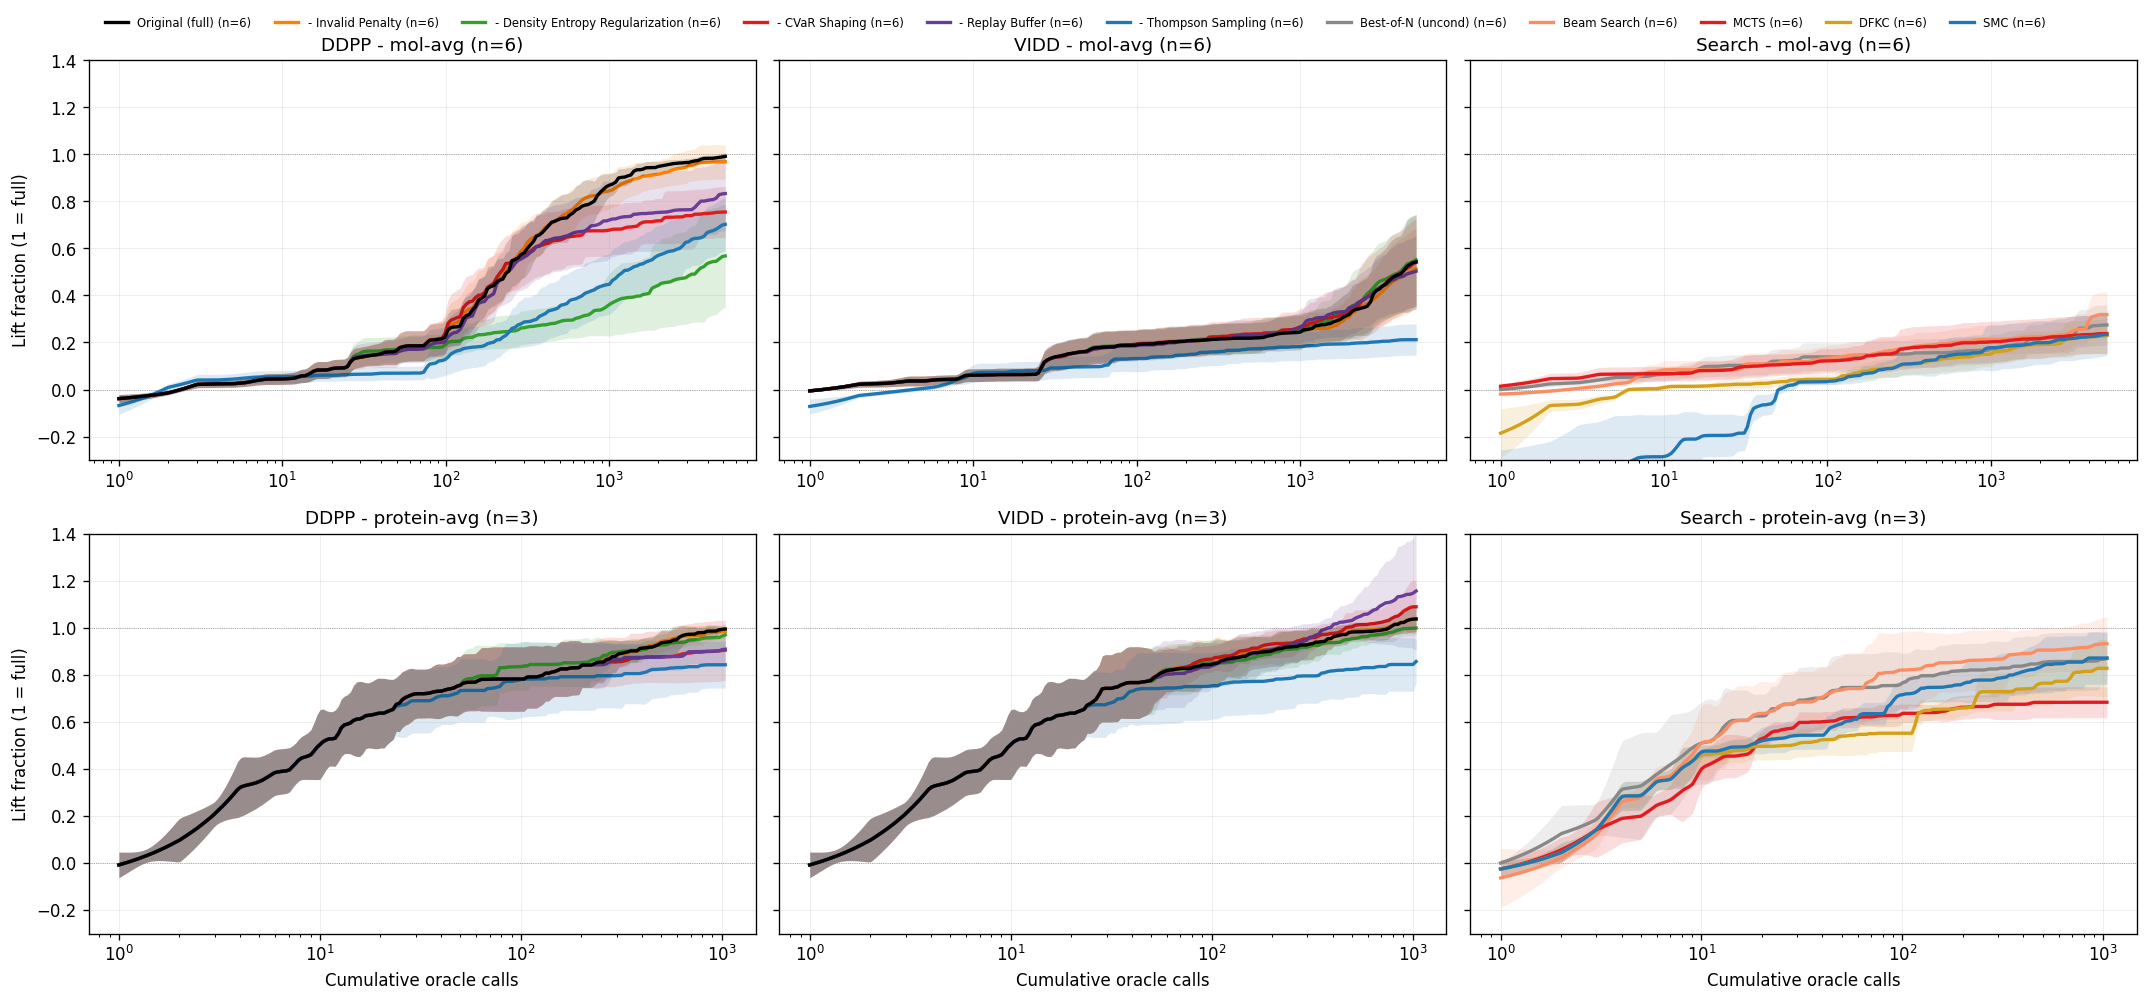
\includegraphics[width=0.95\textwidth]{figures/ablations/avg_grid_norm.png}
  \caption{\textbf{Aggregated ablation grid, oracle-call view.} $2 \times 3$ grid: row $1$ averages over all six FA-oracle small molecules, row $2$ averages over the three protein-fitness families; columns are DDPP-LB ablations, VIDD ablations, and search-only baselines. Same normalised-reward definition as Fig.~\ref{fig:ablation_ddpp}. Across-target CI bands (target-level variability) are wider than the per-target seed bands in the figures above.}
  \label{fig:avg_ablation_calls}
\end{figure}

\begin{figure}[H]
  \centering
  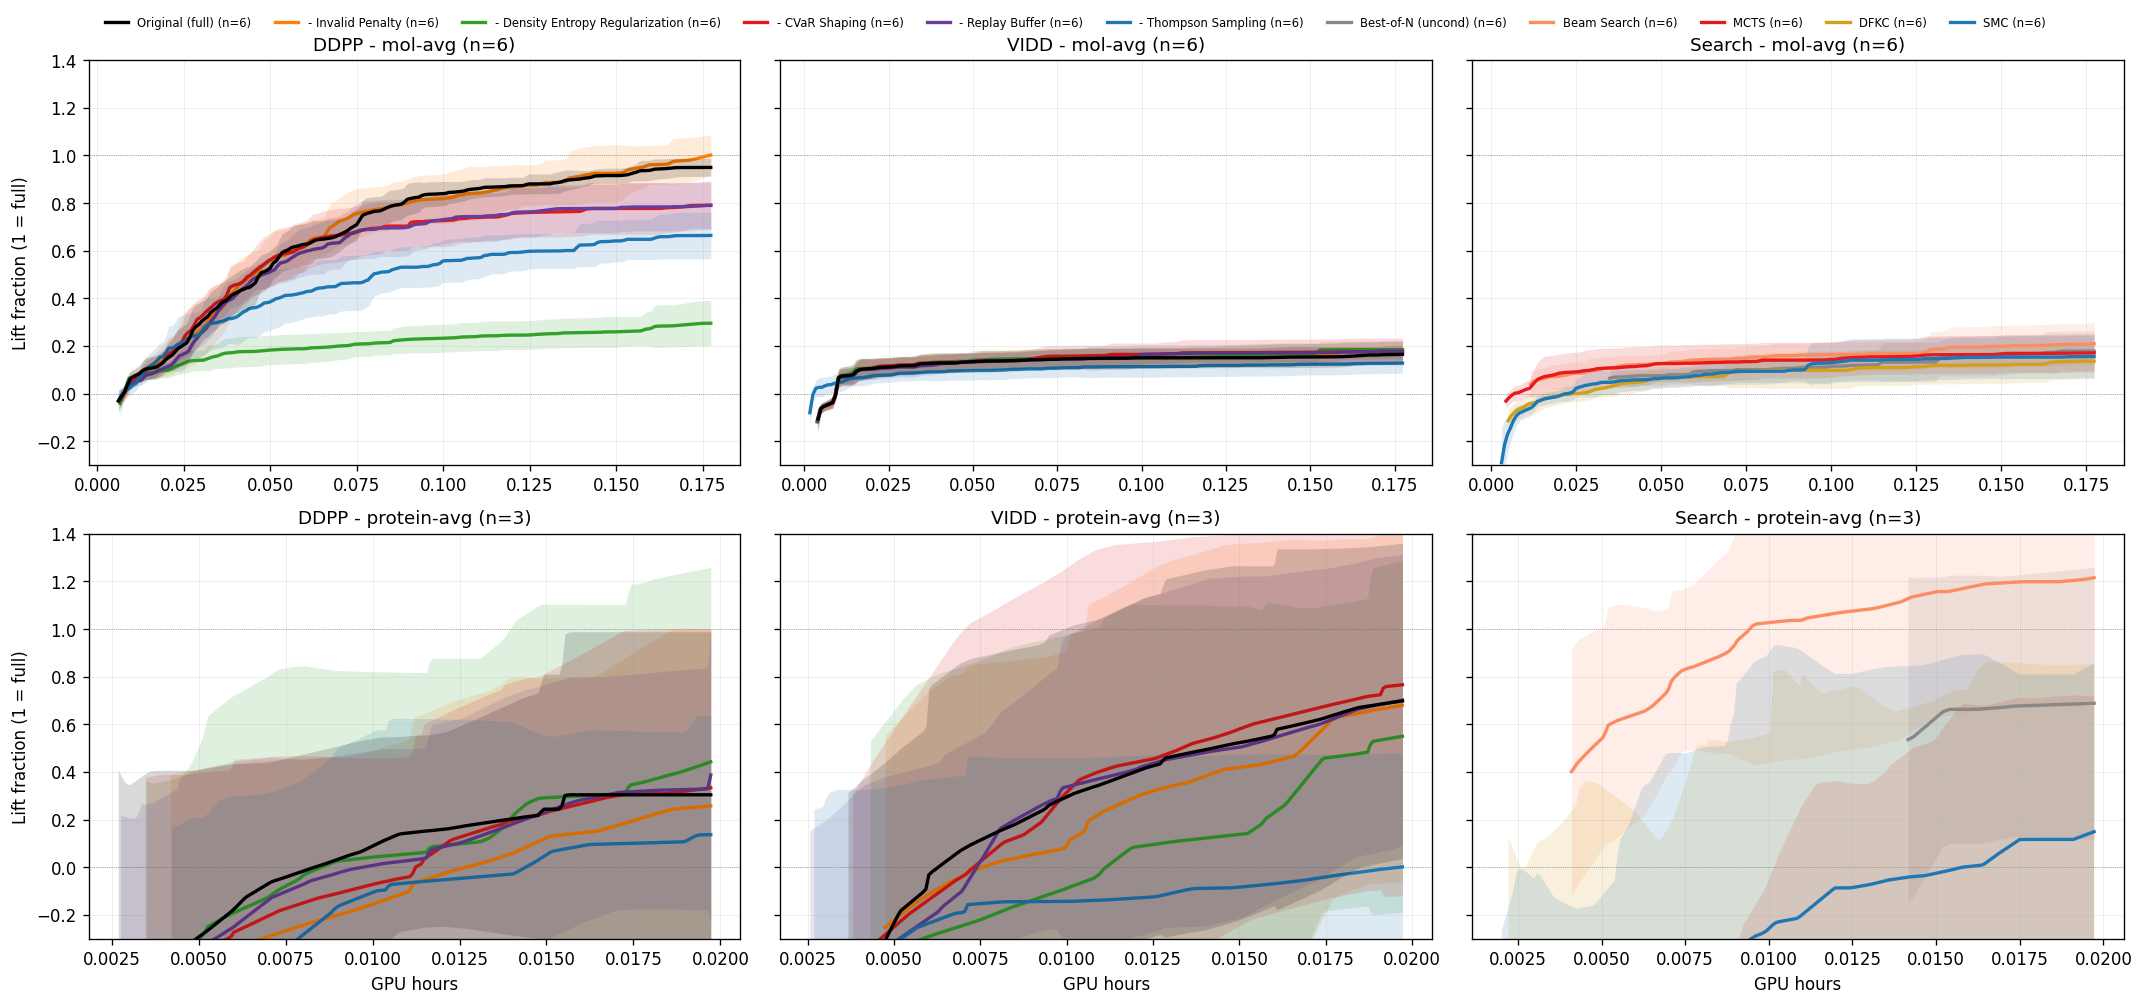
\includegraphics[width=0.95\textwidth]{figures/ablations/avg_grid_norm_gpuhrs.png}
  \caption{\textbf{Aggregated ablation grid, GPU-hours view.} GPU-hours twin of Fig.~\ref{fig:avg_ablation_calls}; same averaging.}
  \label{fig:avg_ablation_gpuhrs}
\end{figure}

% Previous heading: \section{GPU-hour view of the ablation grids}\label{app:gpuhrs-ablation}
\subsection{GPU-Hour View of the Ablation Grids}\label{app:gpuhrs-ablation}

The main-text and per-task ablation grids (Figs.~\ref{fig:ablation_ddpp}, \ref{fig:ablation_search}, \ref{fig:ablation_vidd}, \ref{fig:per_task_mol_set1}, \ref{fig:per_task_mol_set2}, \ref{fig:per_task_protein}) use cumulative oracle calls on the x-axis to isolate feedback efficiency. This appendix replots the same data against GPU hours, including method-side cost (generation, scoring, surrogate update, finetuning); see Sec.~\ref{sec:exp-setup} for the motivation. Same normalised-reward definition throughout.

\begin{figure}[H]
  \centering
  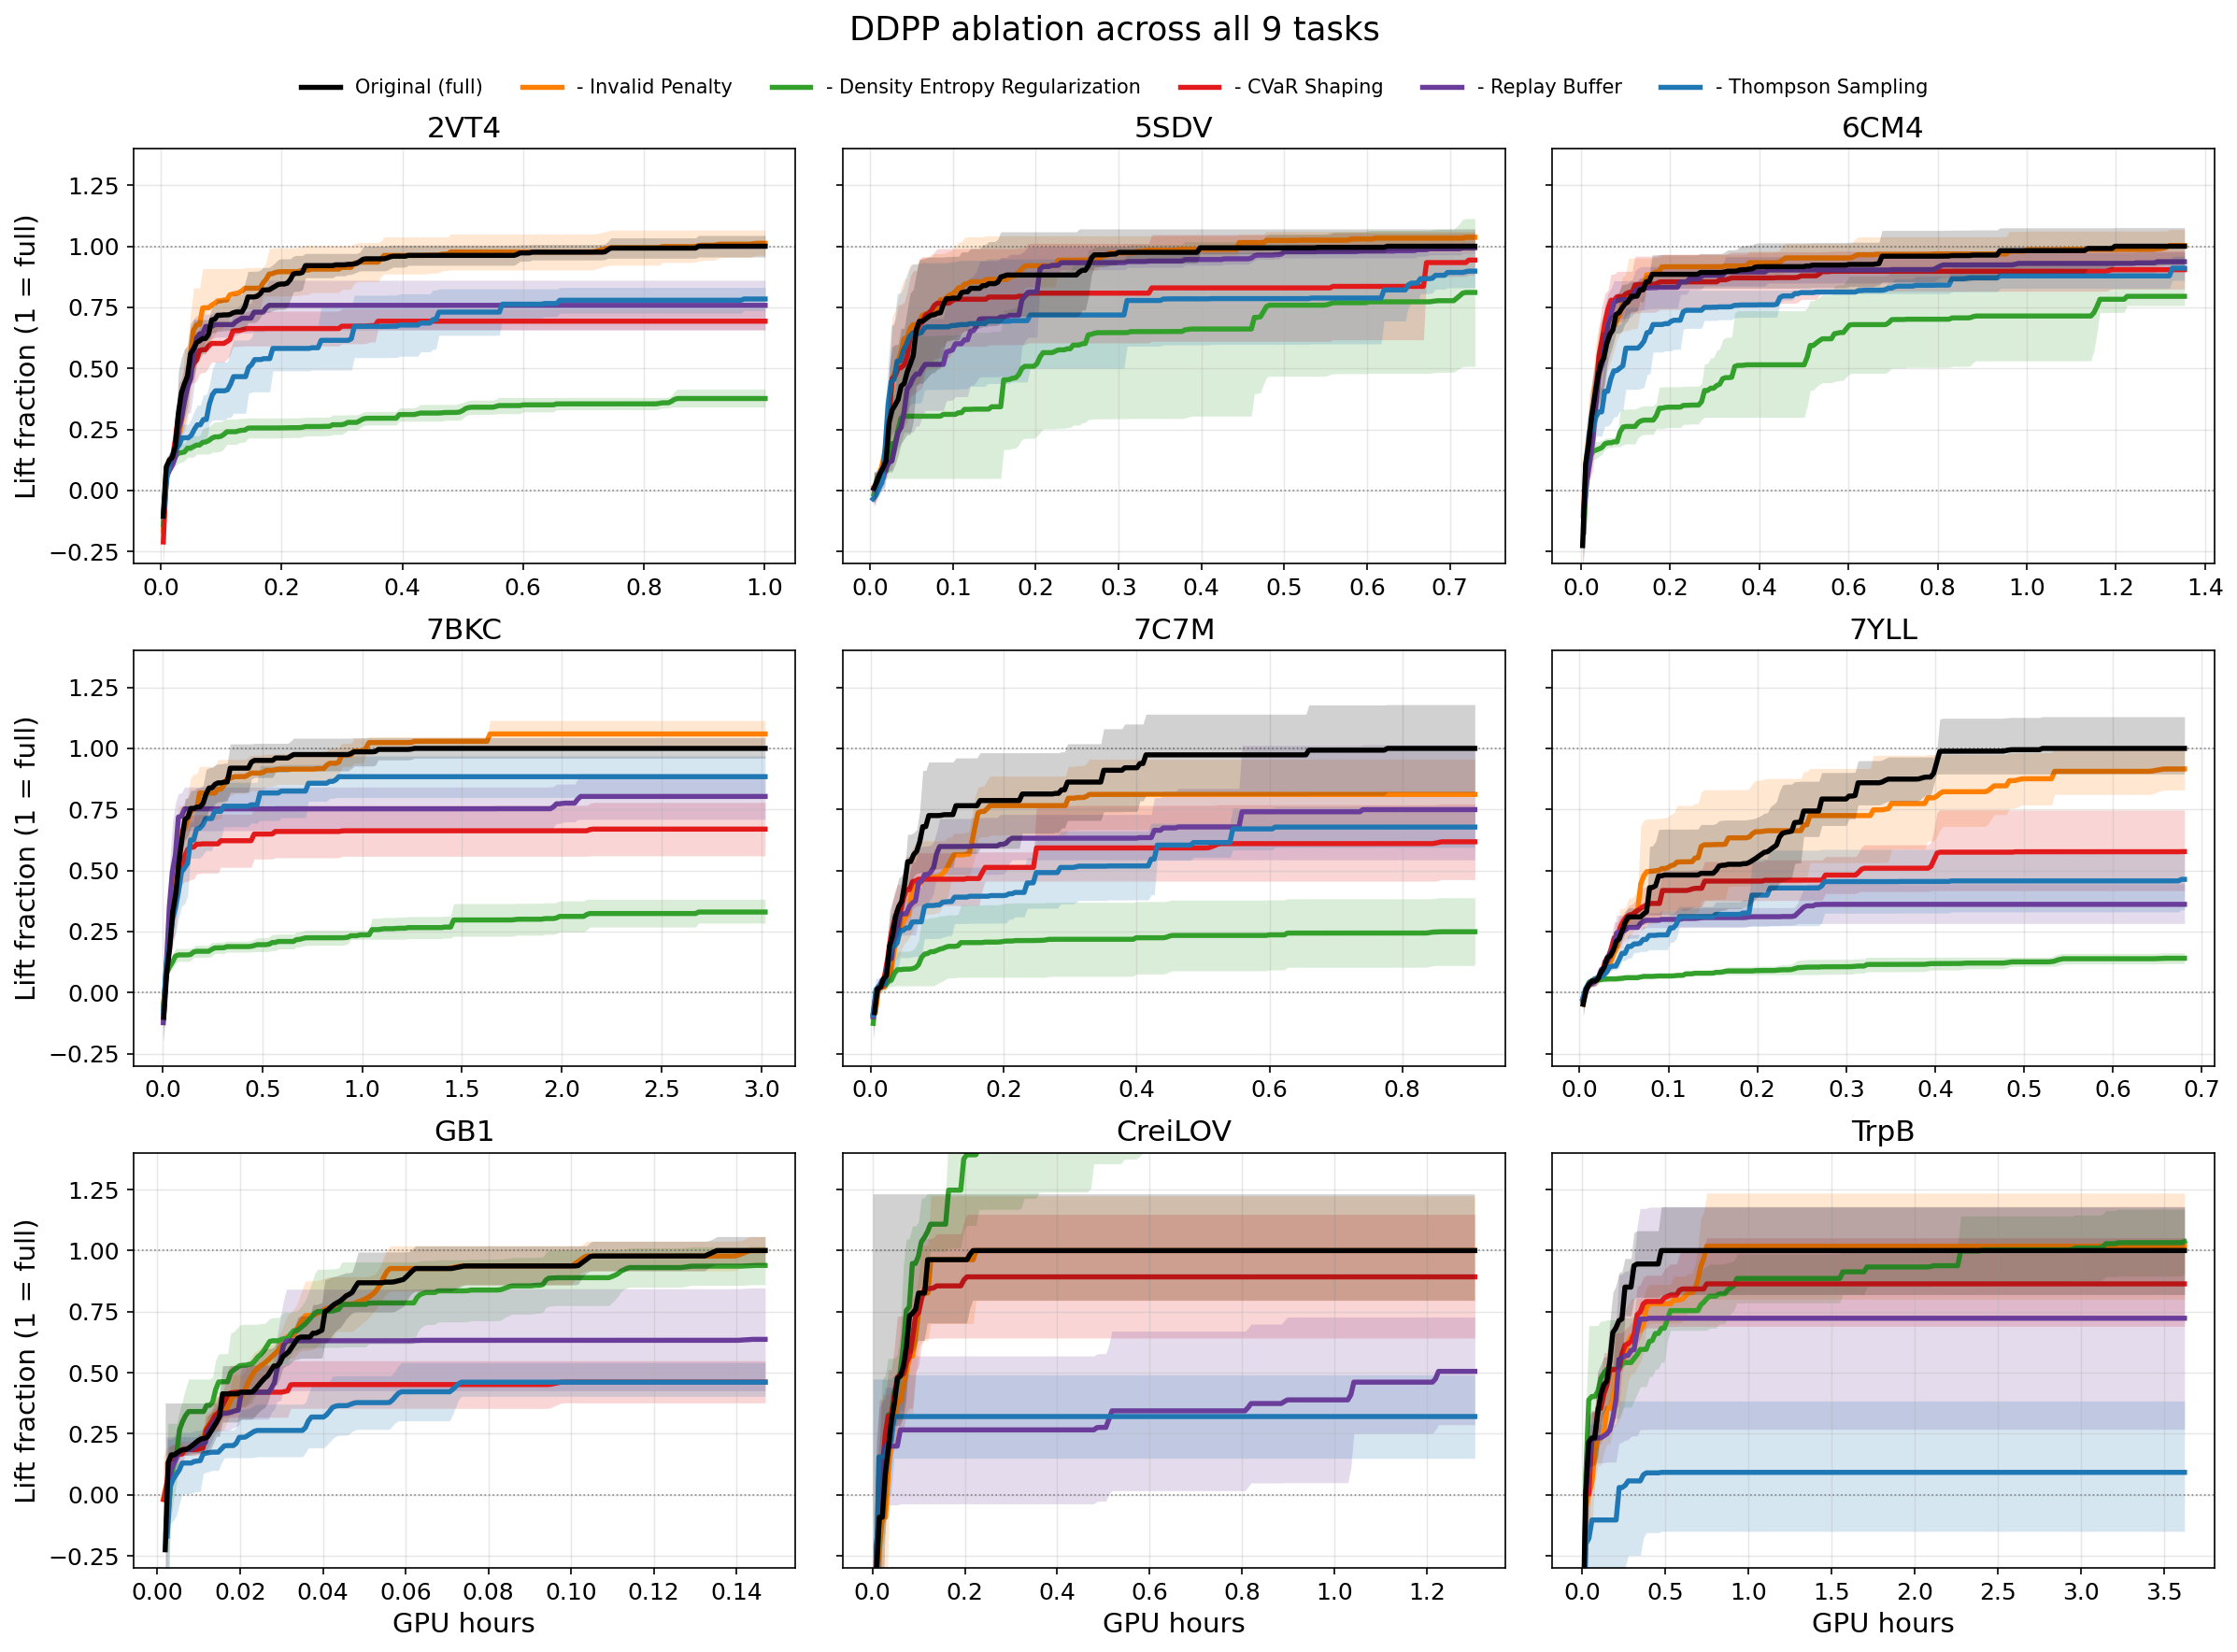
\includegraphics[width=0.95\textwidth]{figures/ablations/ddpp_only_grid_norm_gpuhrs.png}
  \caption{\textbf{DDPP-LB harness ablation, GPU-hours view.} GPU-hours twin of Fig.~\ref{fig:ablation_ddpp}. Knob ordering is largely preserved, but the gap between the full method and \textit{- Thompson sampling} narrows in wall time --- the Thompson step adds non-trivial method-side cost.}
  \label{fig:ablation_ddpp_gpuhrs}
\end{figure}

\begin{figure}[H]
  \centering
  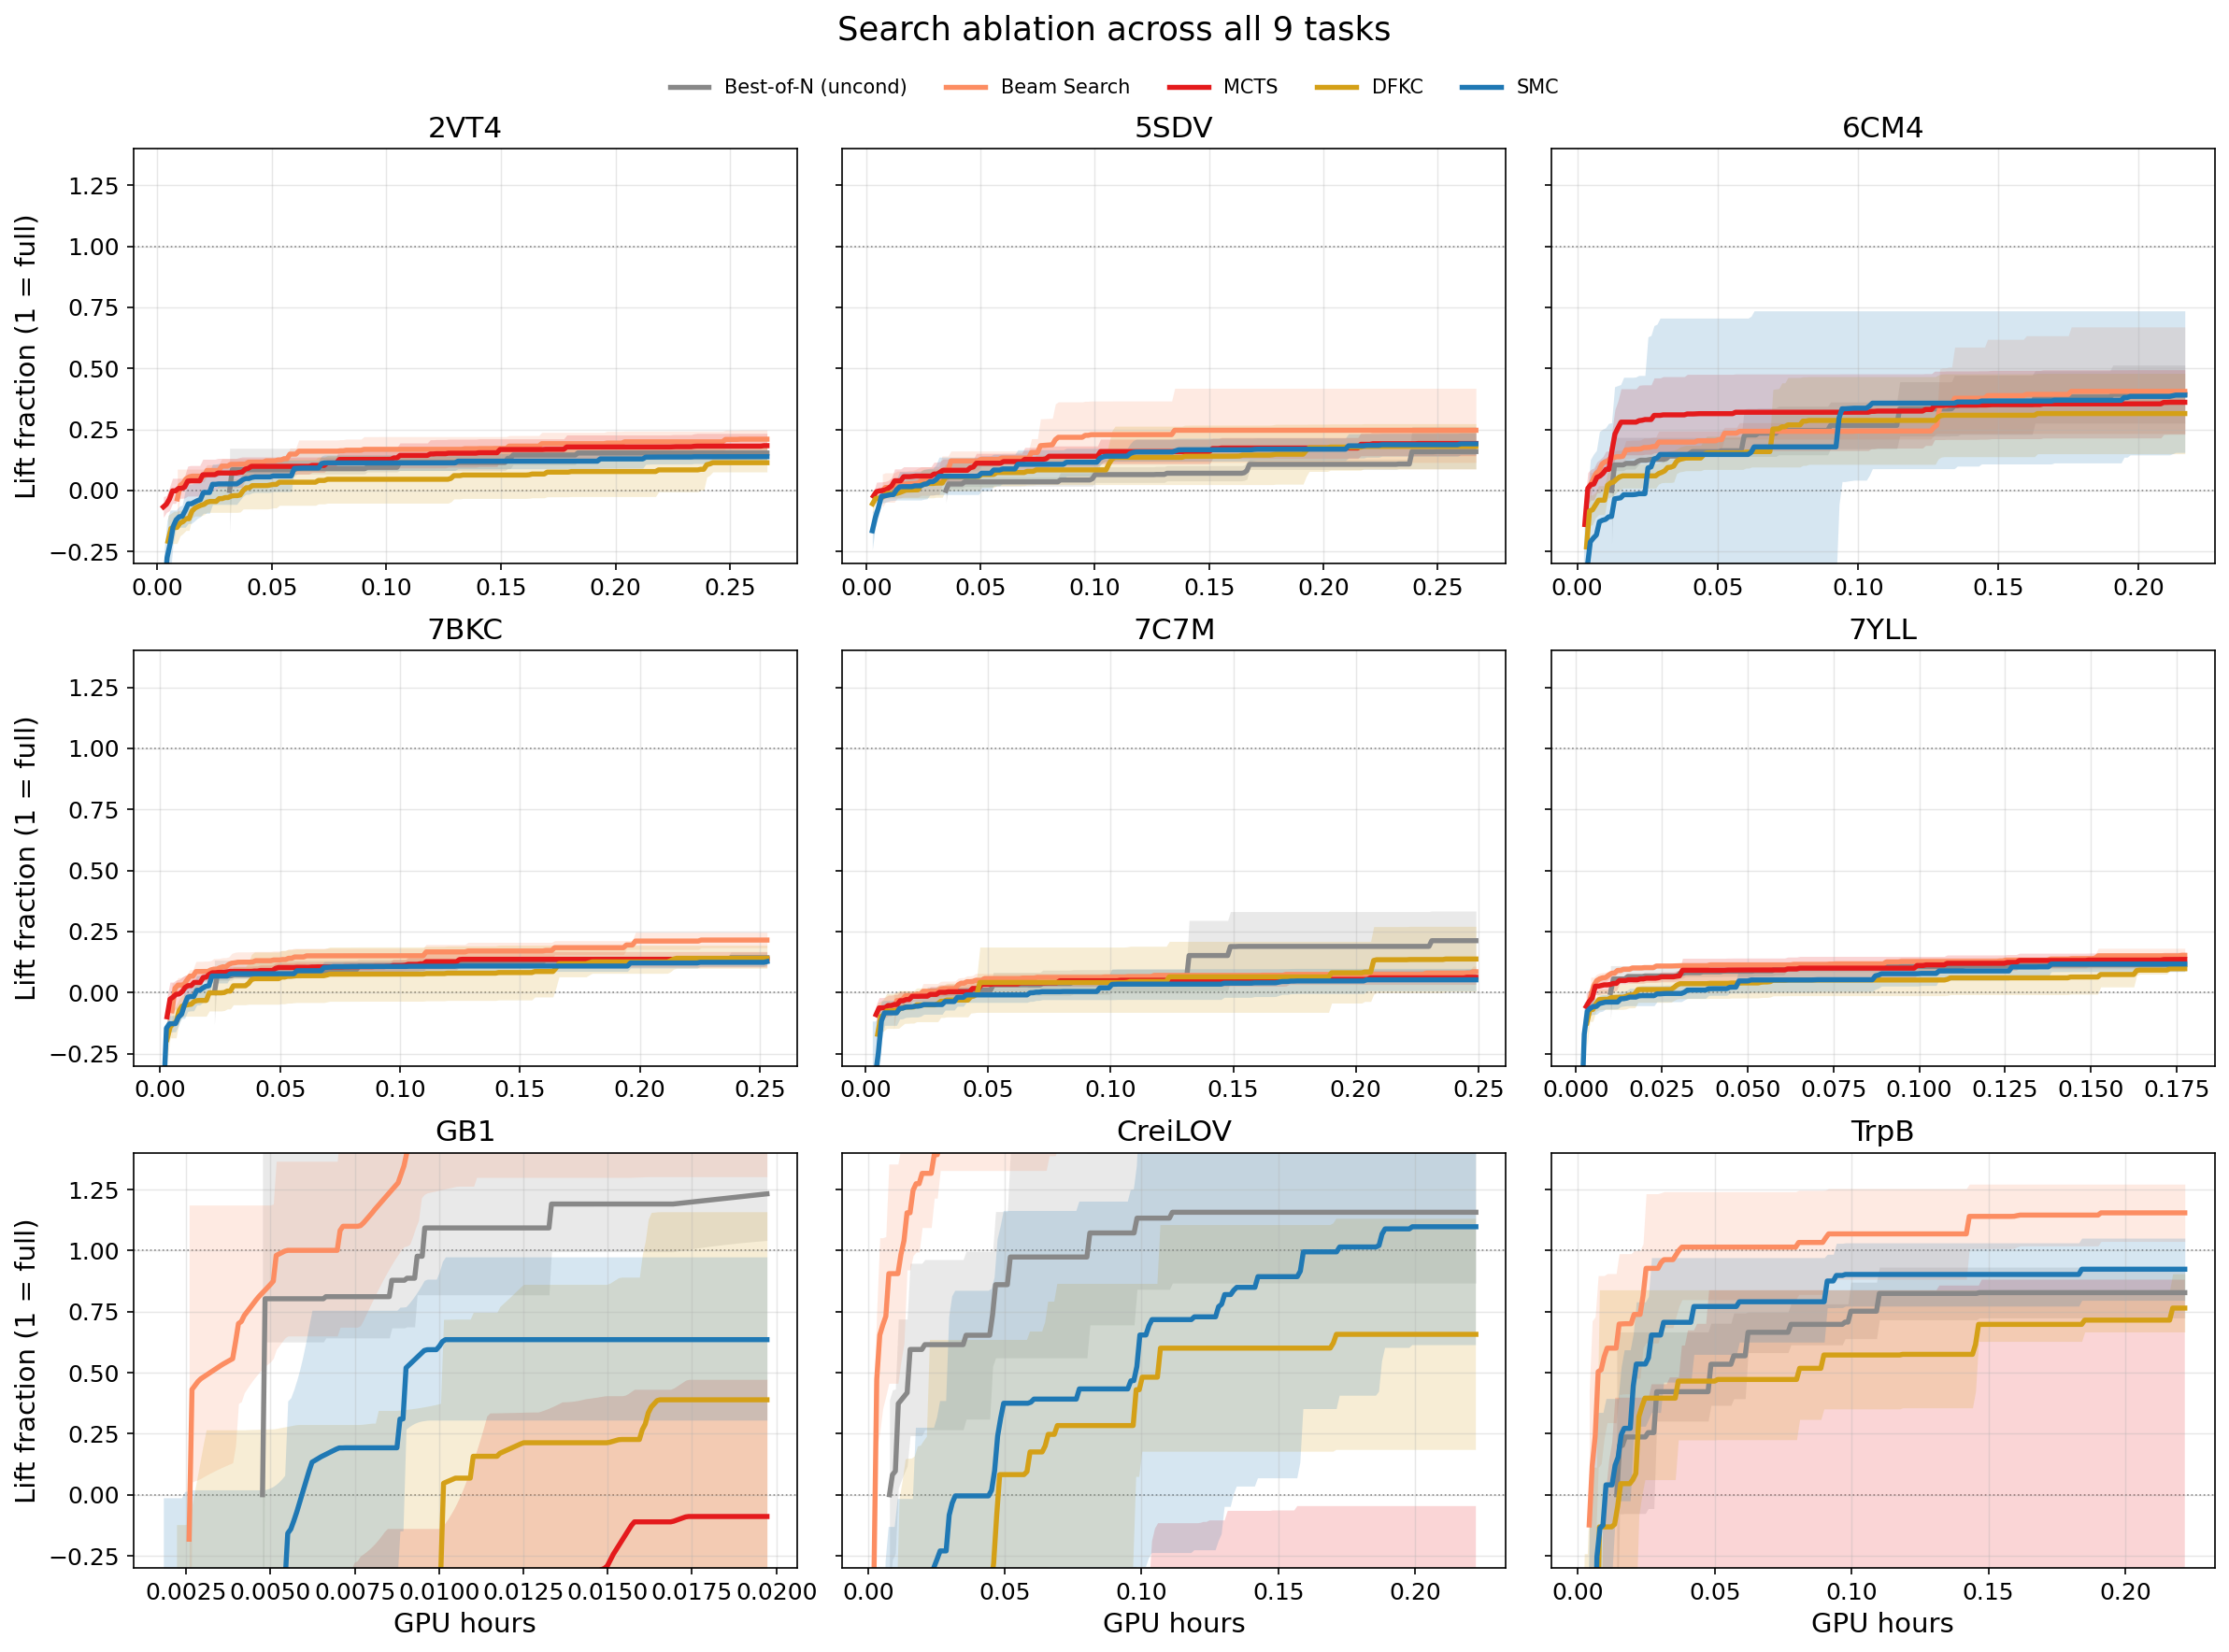
\includegraphics[width=0.95\textwidth]{figures/ablations/search_only_grid_norm_gpuhrs.png}
  \caption{\textbf{Search-only baselines, GPU-hours view.} GPU-hours twin of Fig.~\ref{fig:ablation_search}. Plain best-of-$N$ wins on wall time more often than on oracle-call efficiency --- no per-call surrogate / search overhead.}
  \label{fig:ablation_search_gpuhrs}
\end{figure}

\begin{figure}[H]
  \centering
  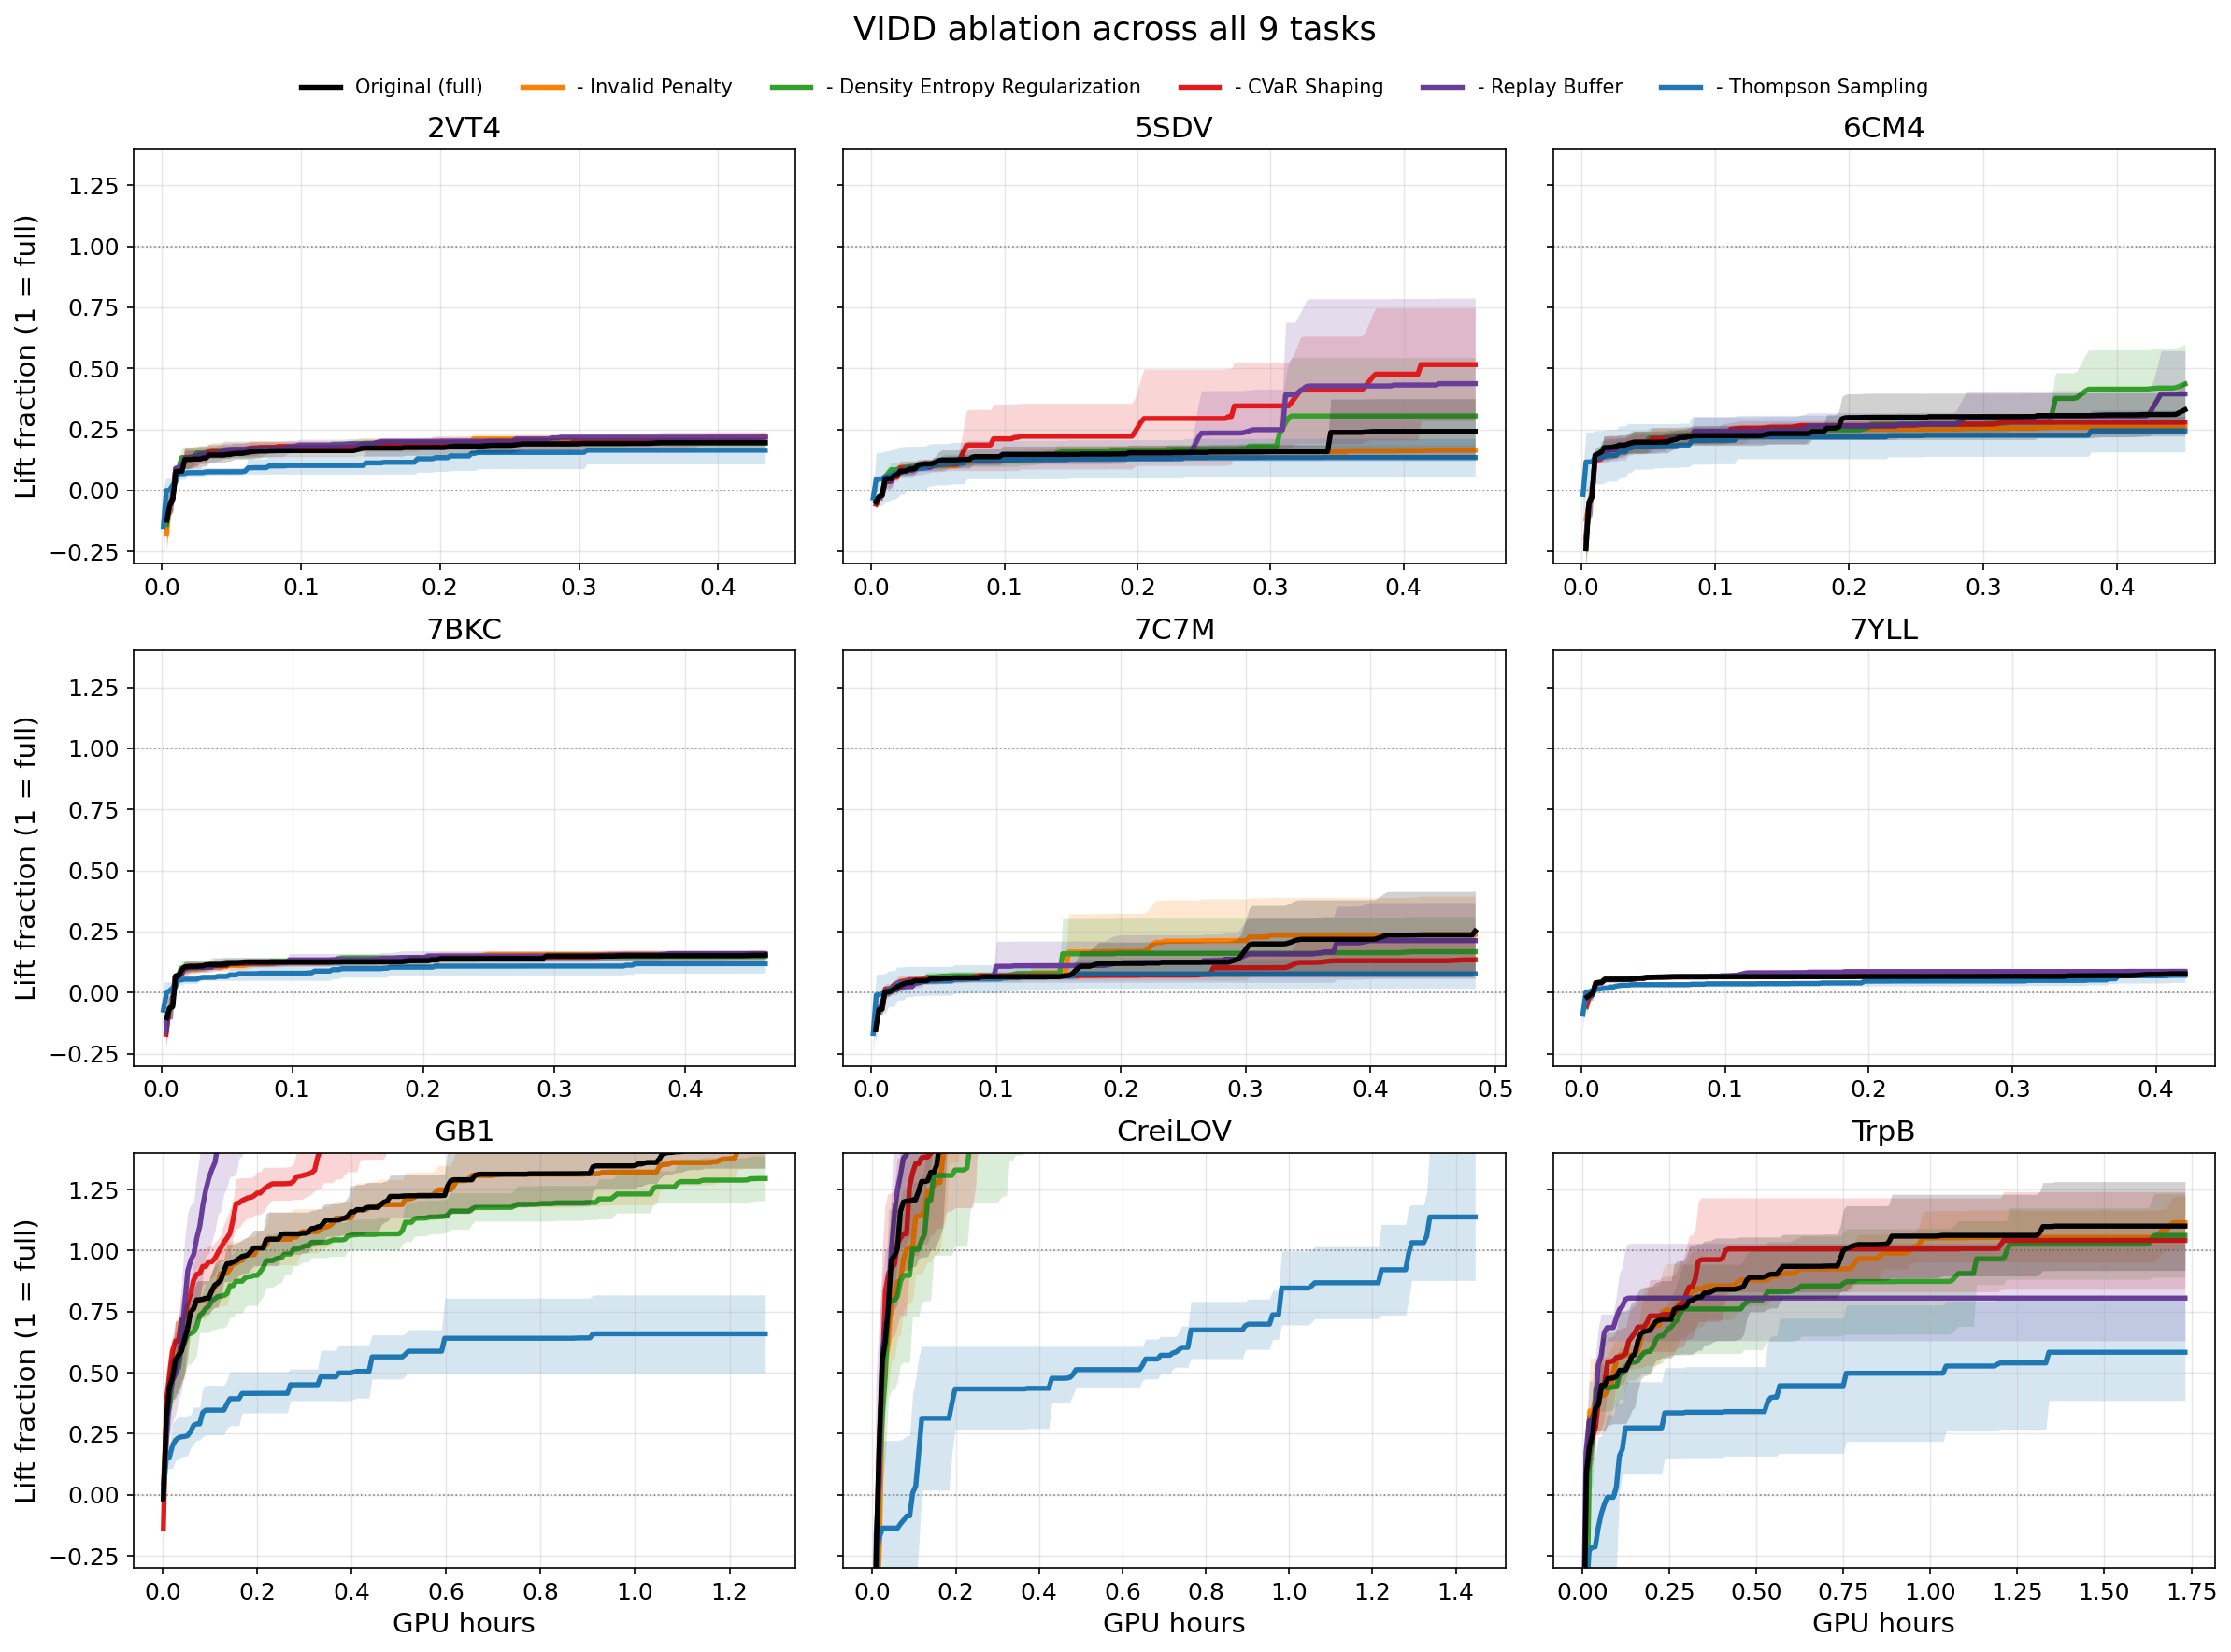
\includegraphics[width=0.95\textwidth]{figures/ablations/vidd_only_grid_norm_gpuhrs.png}
  \caption{\textbf{VIDD harness ablation, GPU-hours view.} GPU-hours twin of Fig.~\ref{fig:ablation_vidd}. The distillation step adds a fixed per-round cost, so GPU-hour caps are tighter than the corresponding DDPP-LB caps on the same target; knob ordering is unchanged.}
  \label{fig:ablation_vidd_gpuhrs}
\end{figure}

\begin{figure}[H]
  \centering
  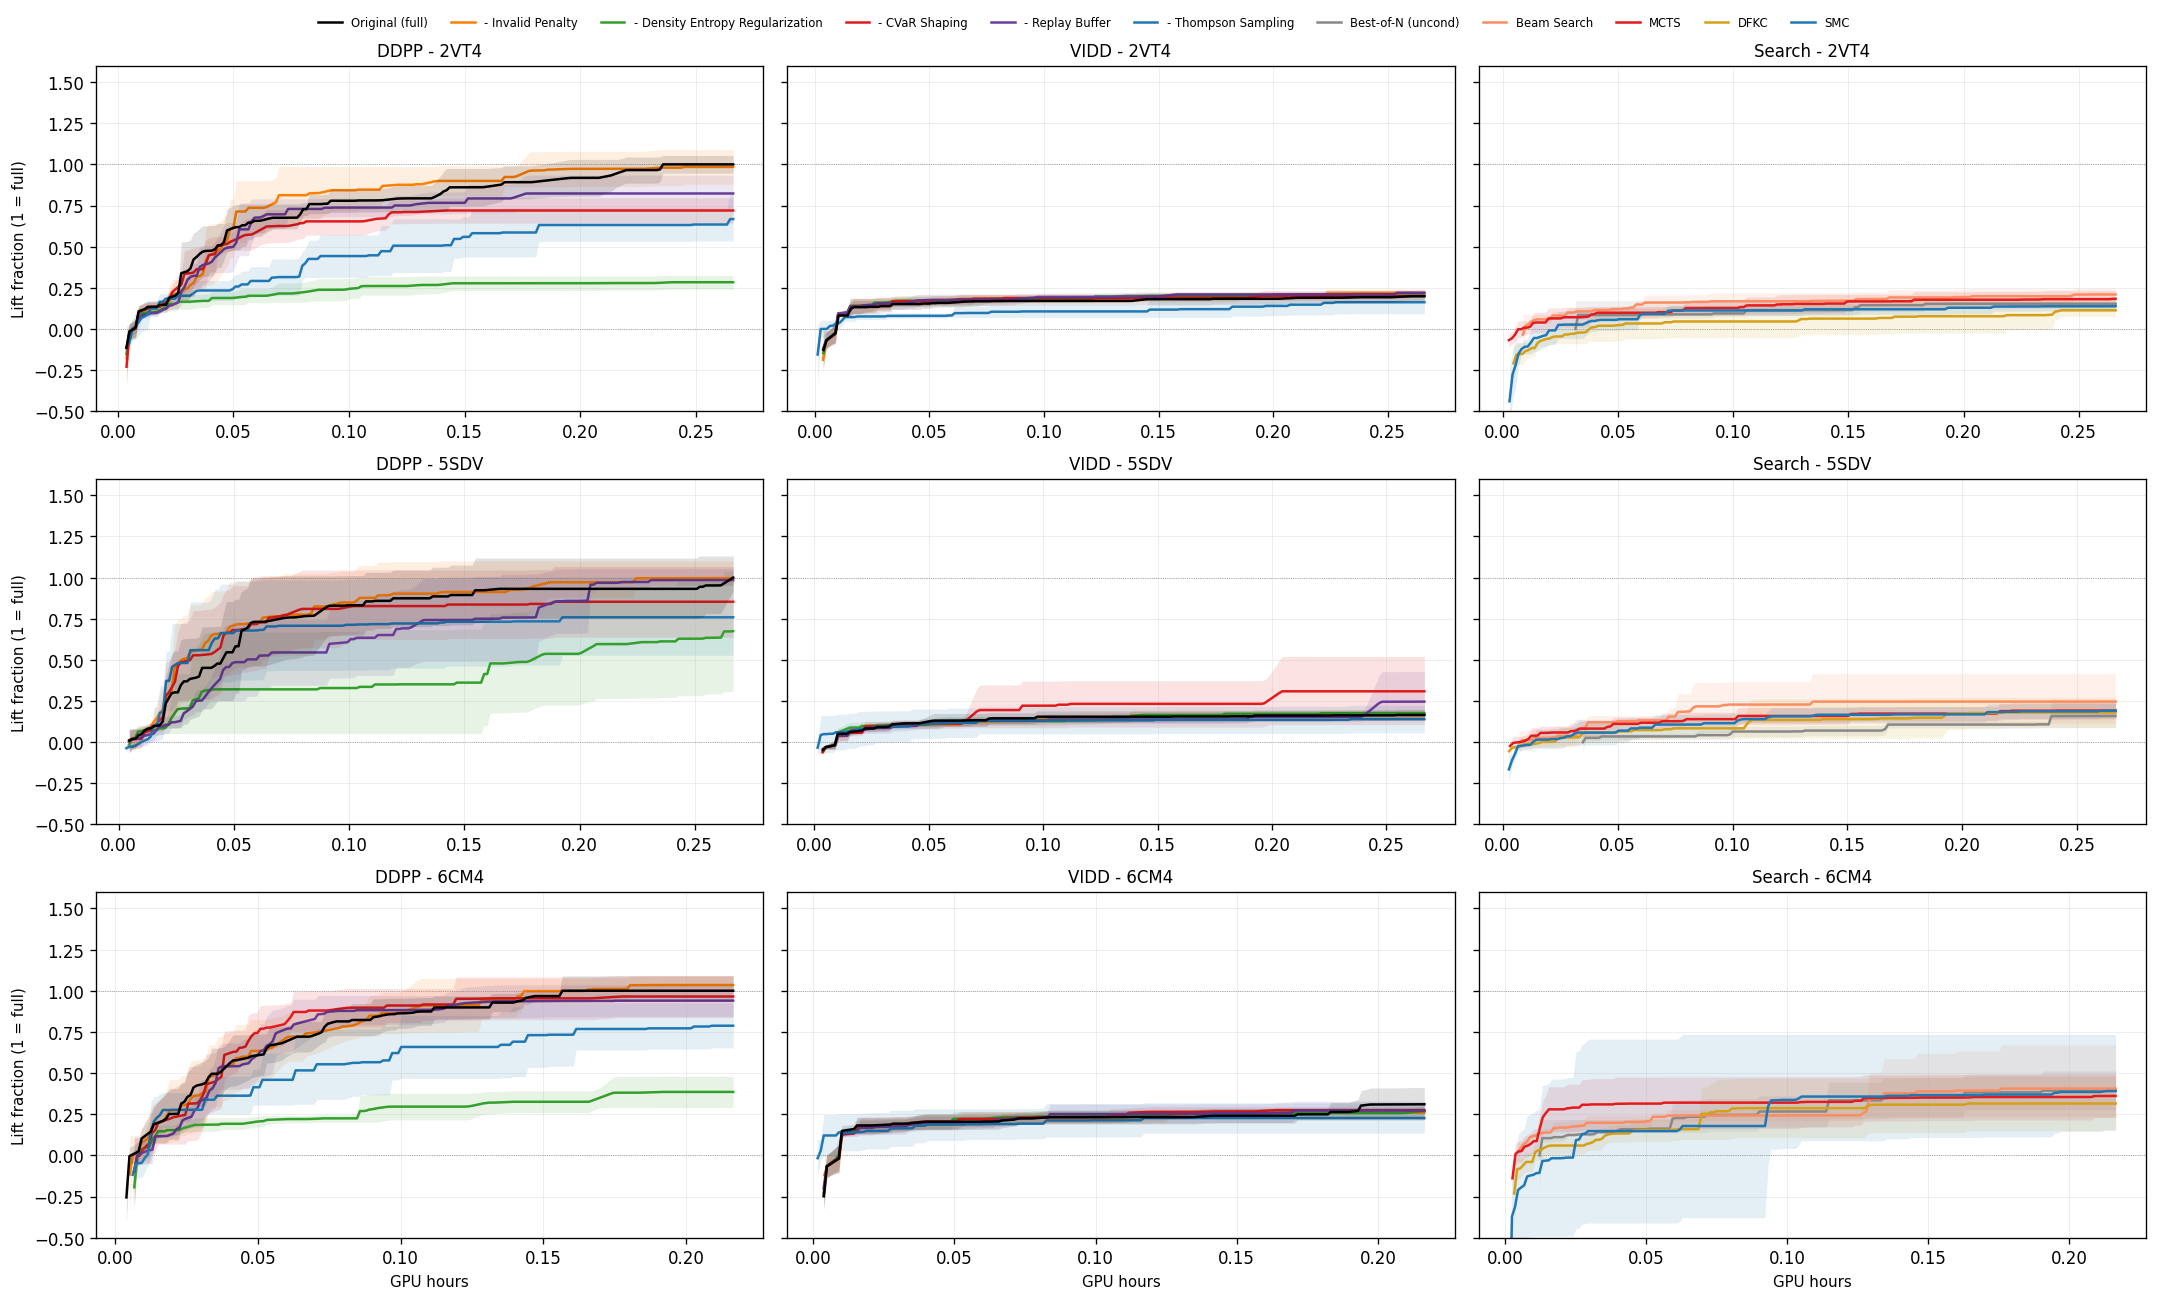
\includegraphics[width=0.95\textwidth]{figures/ablations/mol_ablations_grid_set1_norm_gpuhrs.png}
  \caption{\textbf{Per-task ablation (mol set 1), GPU-hours view.} GPU-hour twin of Fig.~\ref{fig:per_task_mol_set1}.}
  \label{fig:per_task_mol_set1_gpuhrs}
\end{figure}

\begin{figure}[H]
  \centering
  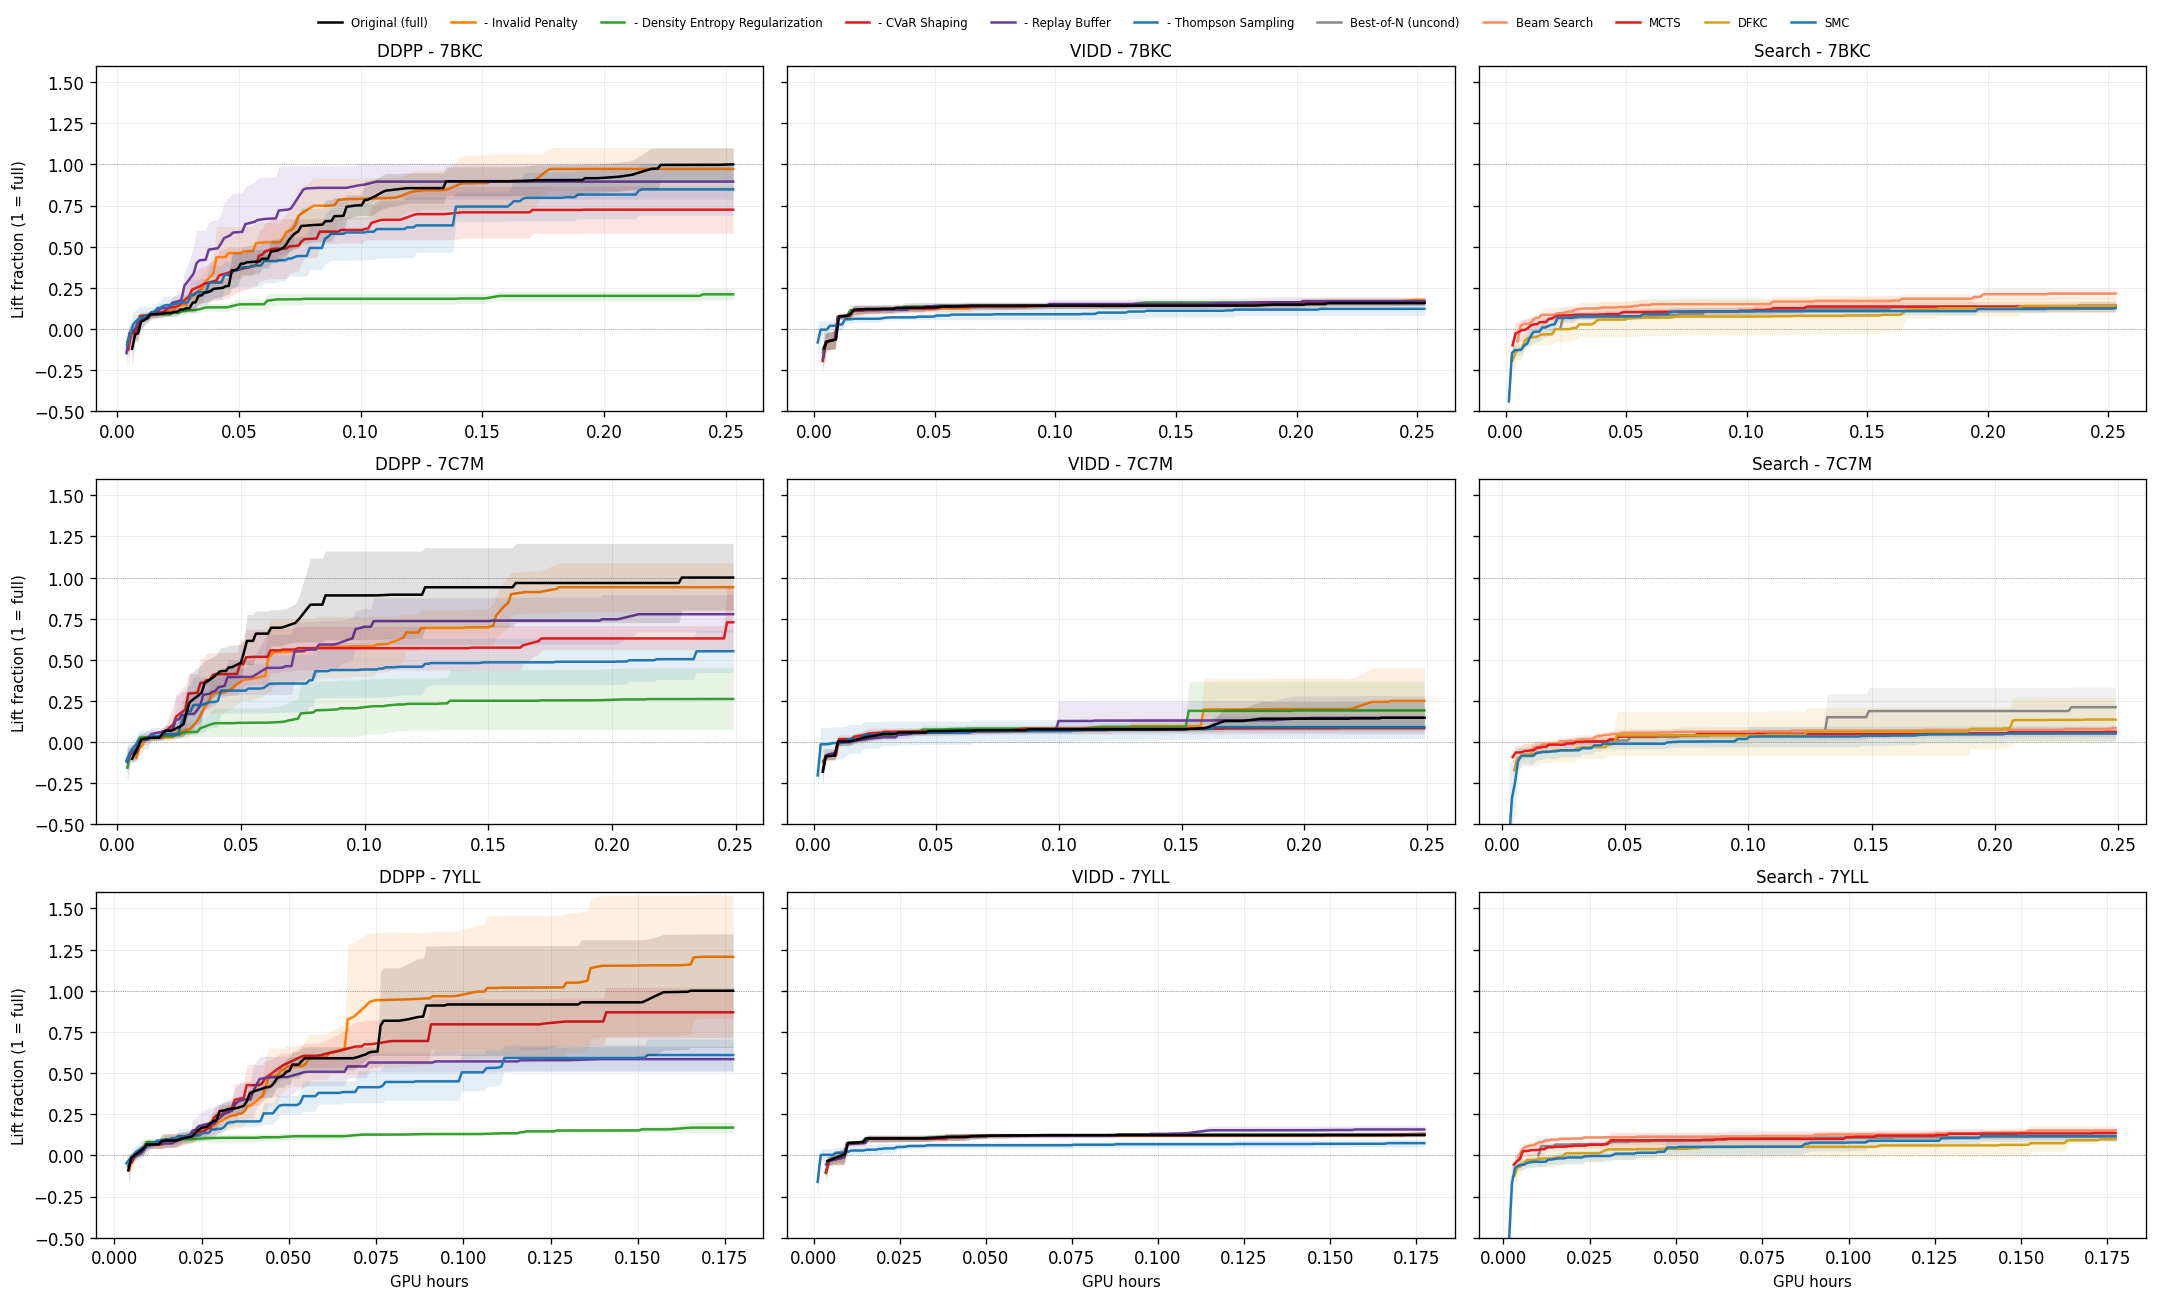
\includegraphics[width=0.95\textwidth]{figures/ablations/mol_ablations_grid_set2_norm_gpuhrs.png}
  \caption{\textbf{Per-task ablation (mol set 2), GPU-hours view.} GPU-hour twin of Fig.~\ref{fig:per_task_mol_set2}.}
  \label{fig:per_task_mol_set2_gpuhrs}
\end{figure}

\begin{figure}[H]
  \centering
  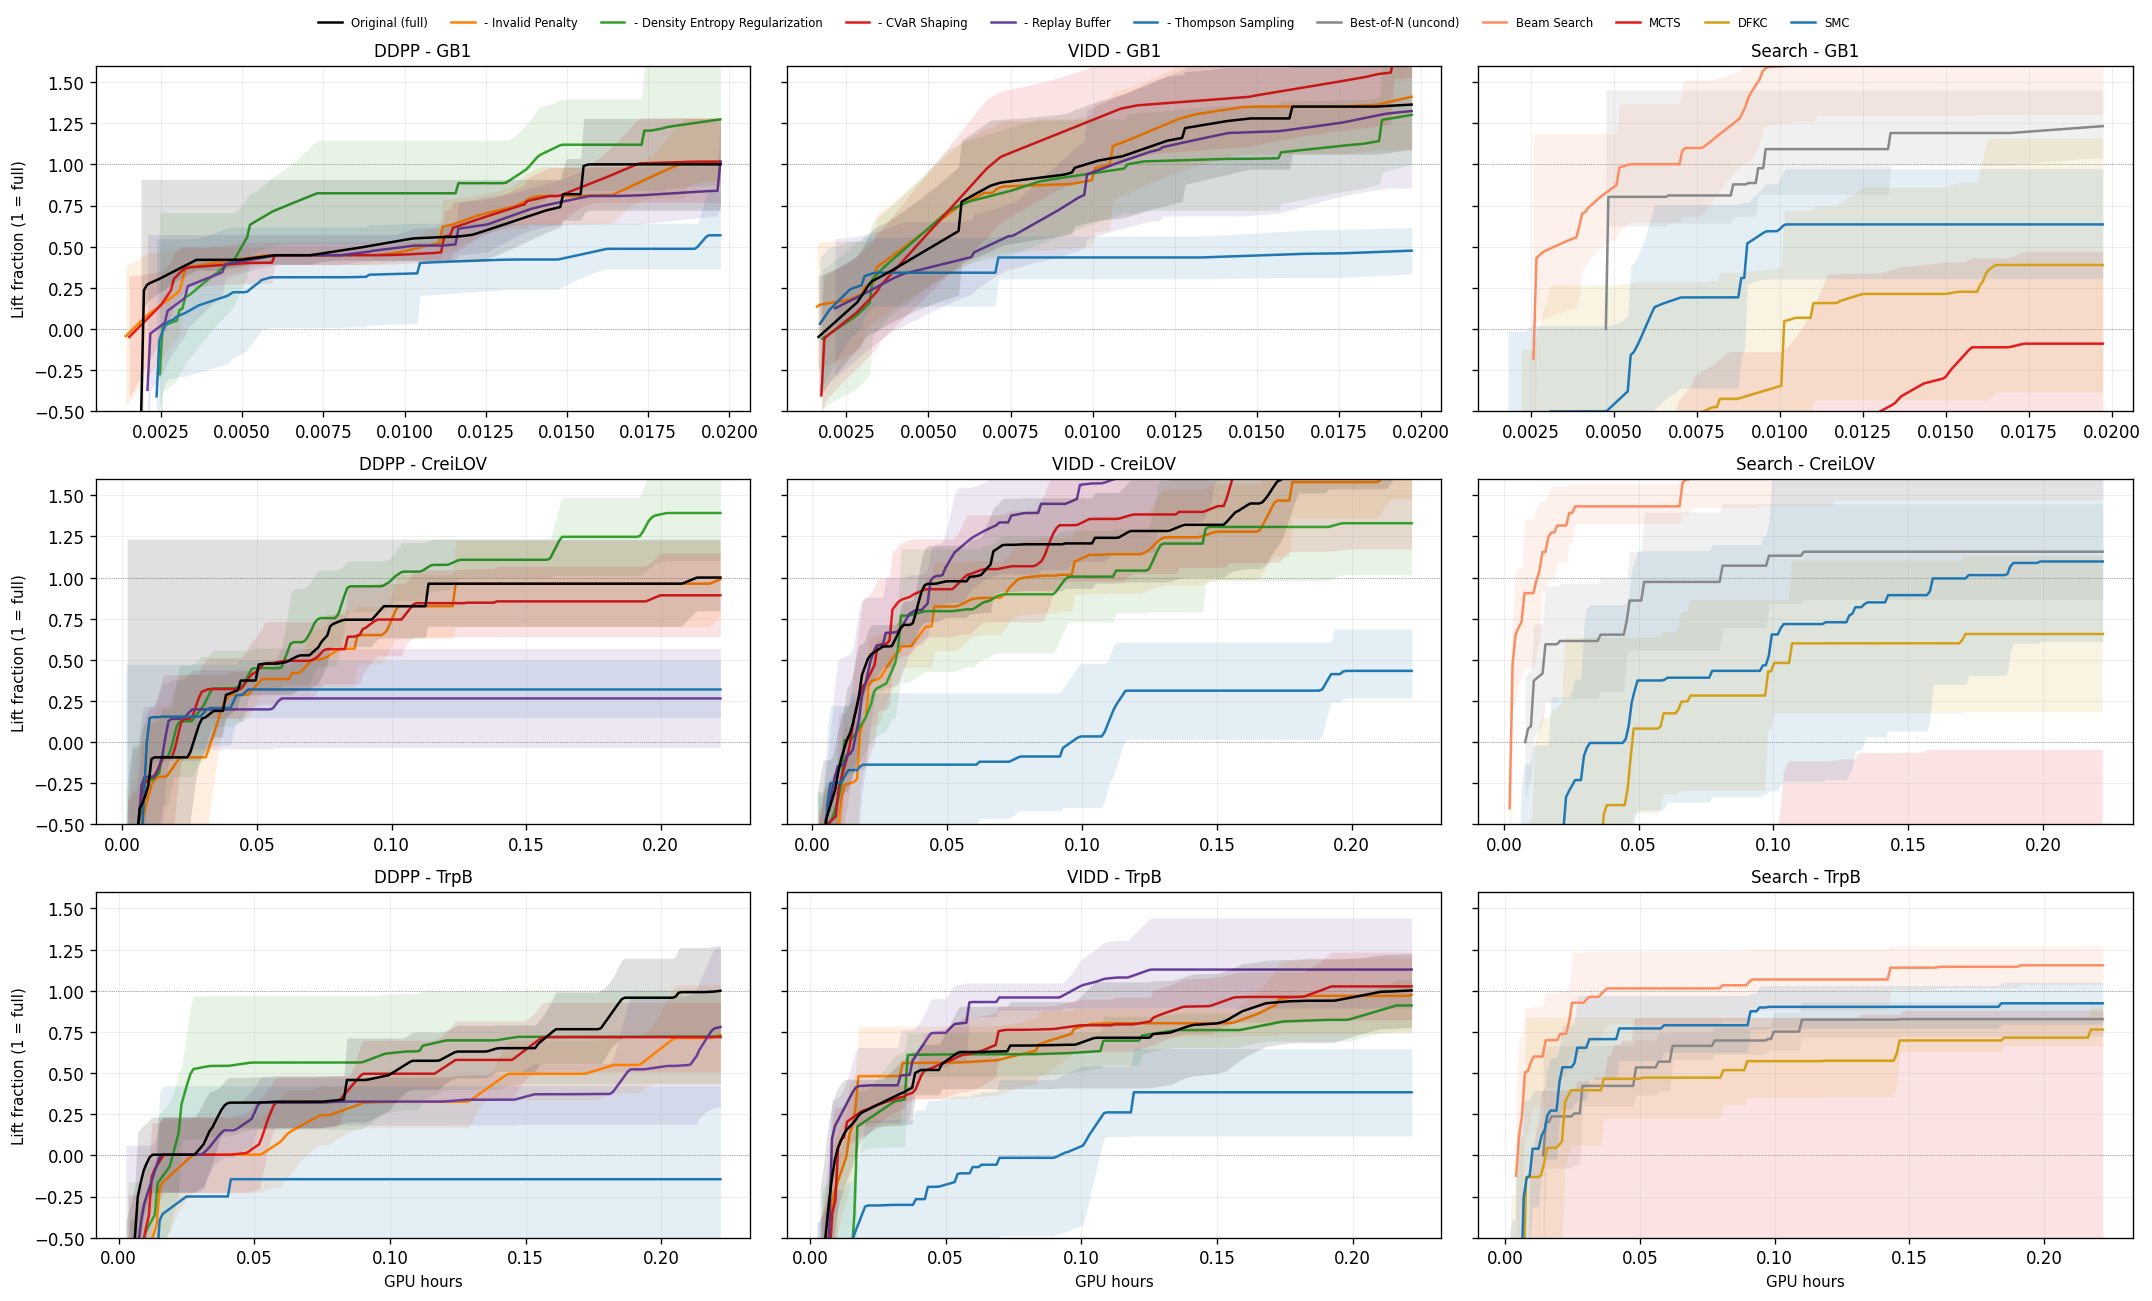
\includegraphics[width=0.95\textwidth]{figures/ablations/protein_ablations_grid_norm_gpuhrs.png}
  \caption{\textbf{Per-task ablation (proteins), GPU-hours view.} GPU-hour twin of Fig.~\ref{fig:per_task_protein}.}
  \label{fig:per_task_protein_gpuhrs}
\end{figure}

% \section{Reproductions of the body bar plots}

% Previous heading: \section{Guide to the main-text bar plots}\label{app:per-target-grids}
\subsection{Guide to the Main-Text Bar Plots}\label{app:per-target-grids}

The canonical bar plots are Fig.~\ref{fig:barplot_ablation} (component ablations) and Fig.~\ref{fig:barplot_inference_search} (full configuration versus search baselines) in the main text. They are referenced directly rather than reproduced here.

% Duplicate main-text bar plots; retained below for recovery.
% Reproducing the body bar plots here so downstream cross-references (per-finetuner discussion, GPU-hours twins, etc.) resolve to a single canonical pair of labels.
% 
% \begin{figure}[H]
%   \centering
%   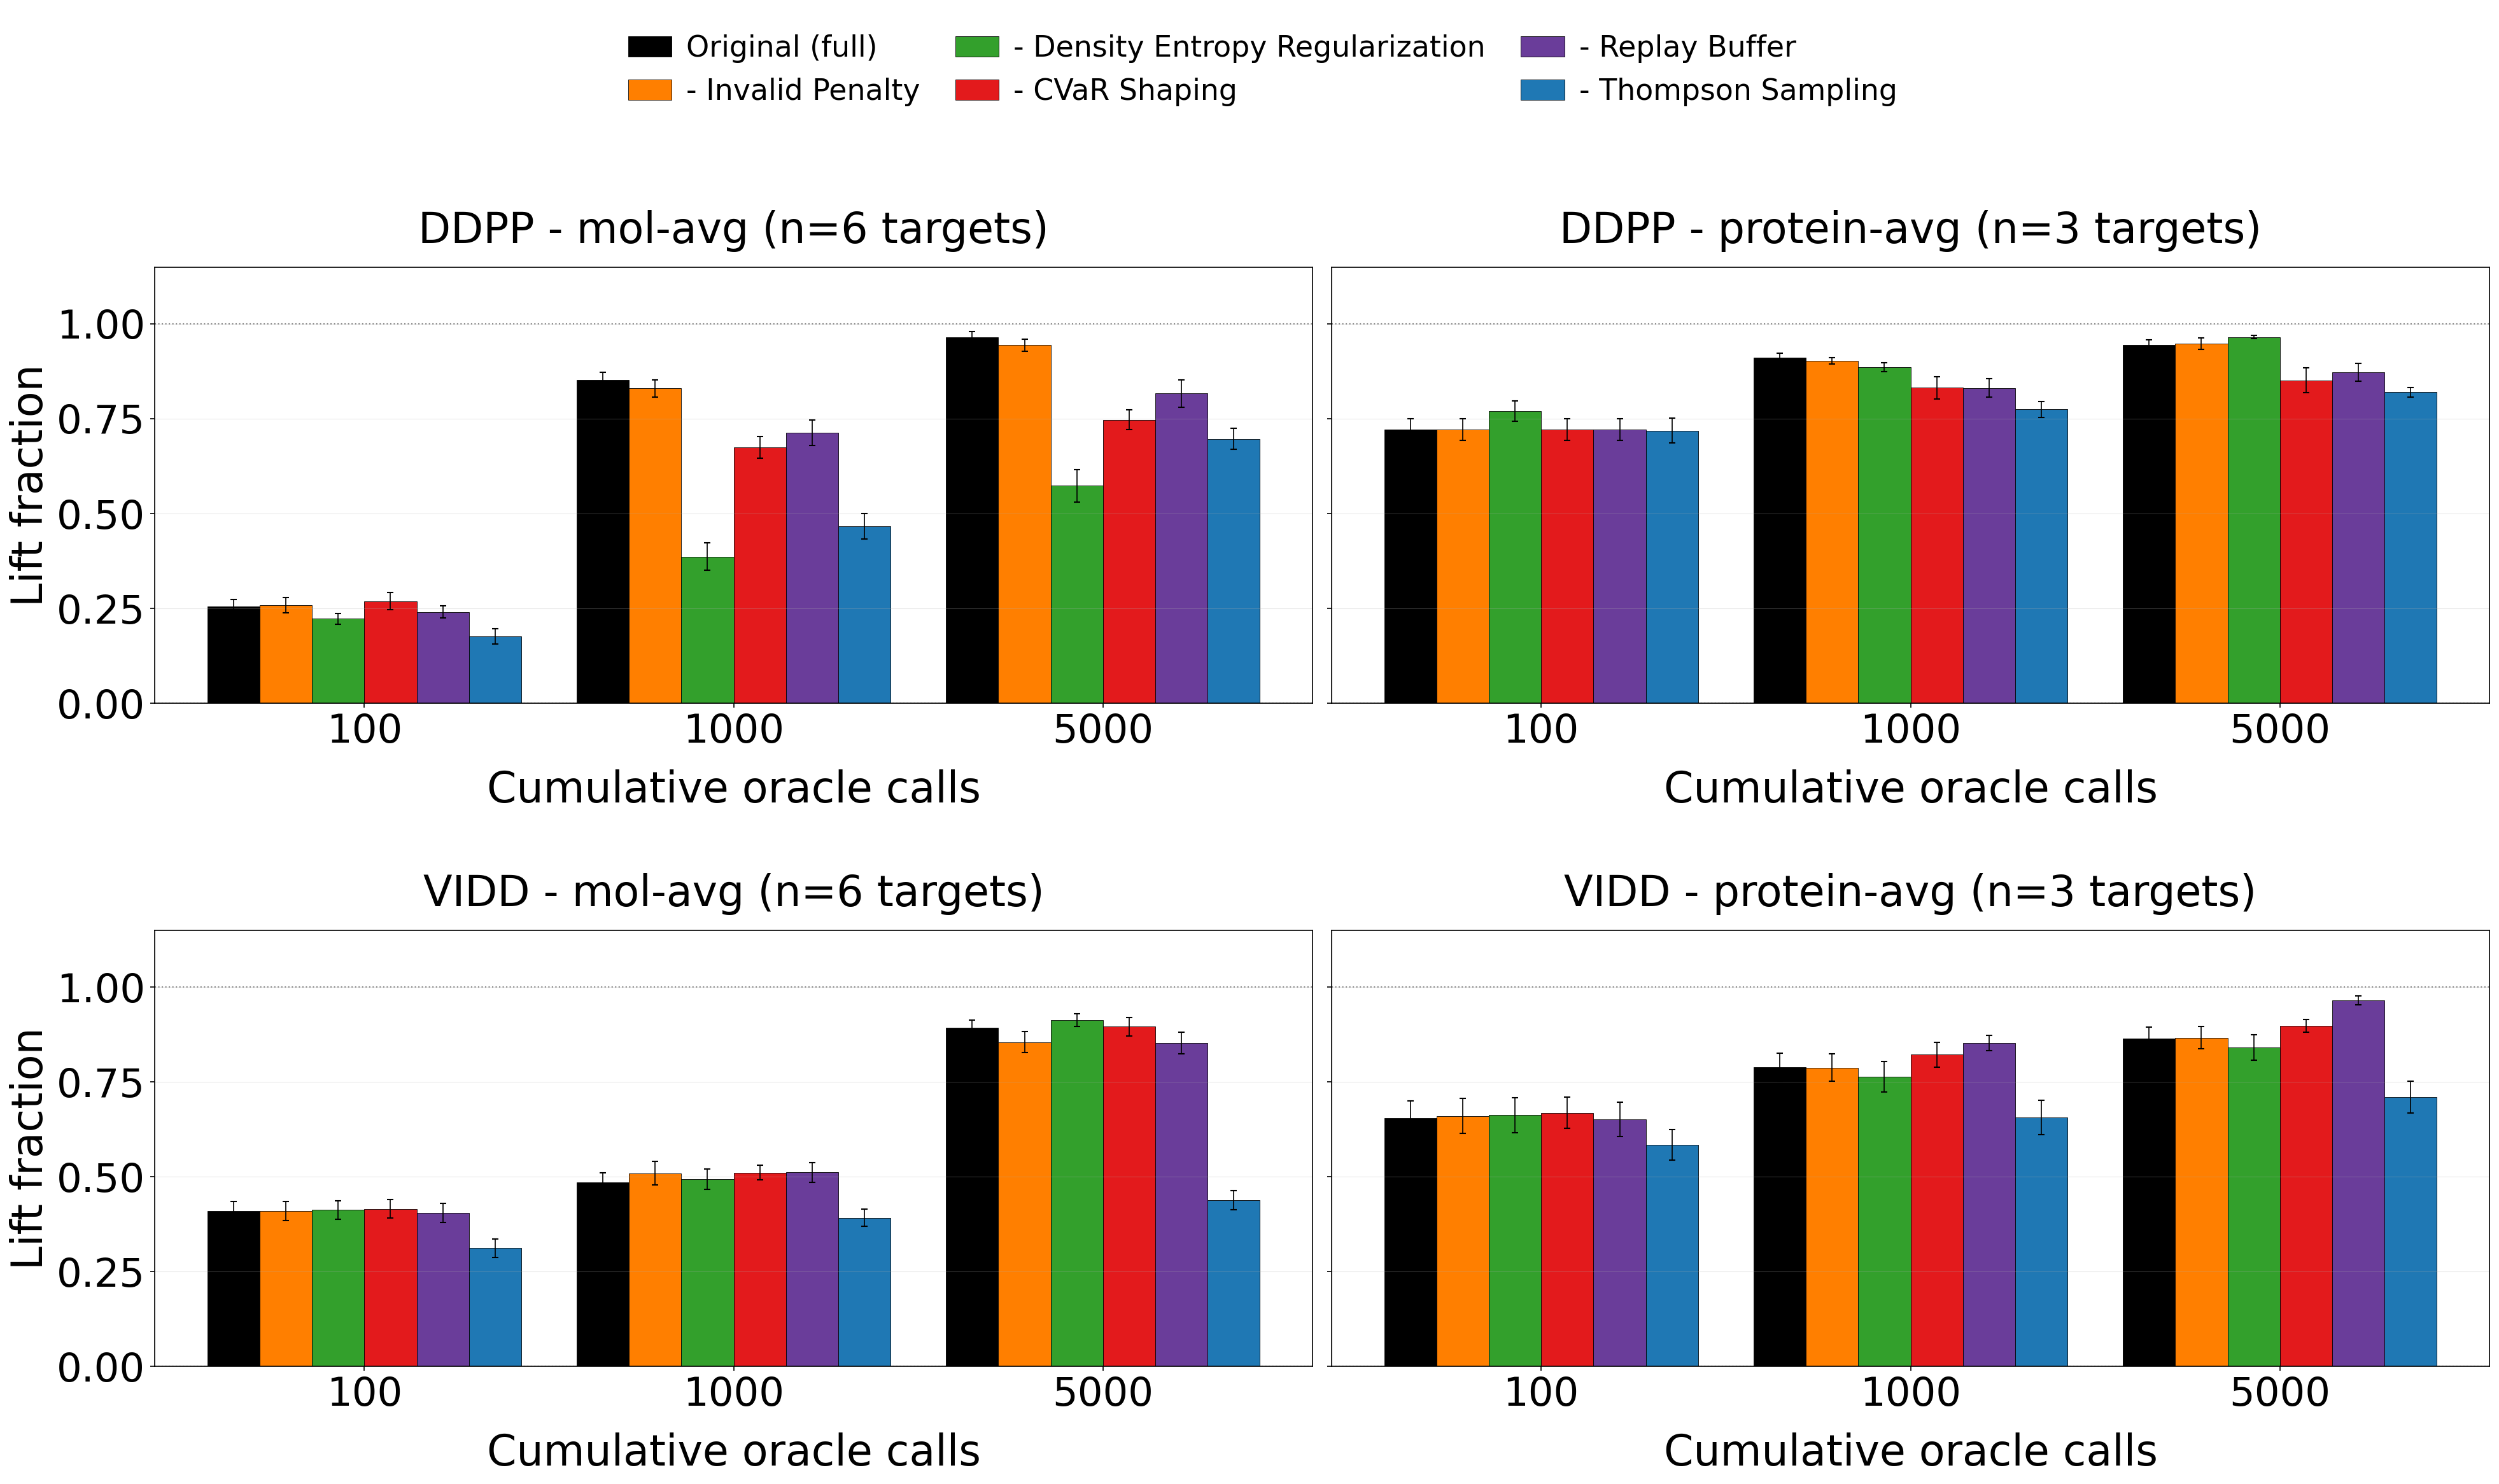
\includegraphics[width=\textwidth]{figures/ablations/result1_combined_vs_baseline.png}
%   \caption{\textbf{DDPP-LB and VIDD harness ablation, normalised-reward bar version.} Reproduces Fig.~\ref{fig:barplot_ablation} for appendix cross-referencing. See body for the full caption and discussion.}
% \end{figure}
% 
% \begin{figure}[H]
%   \centering
%   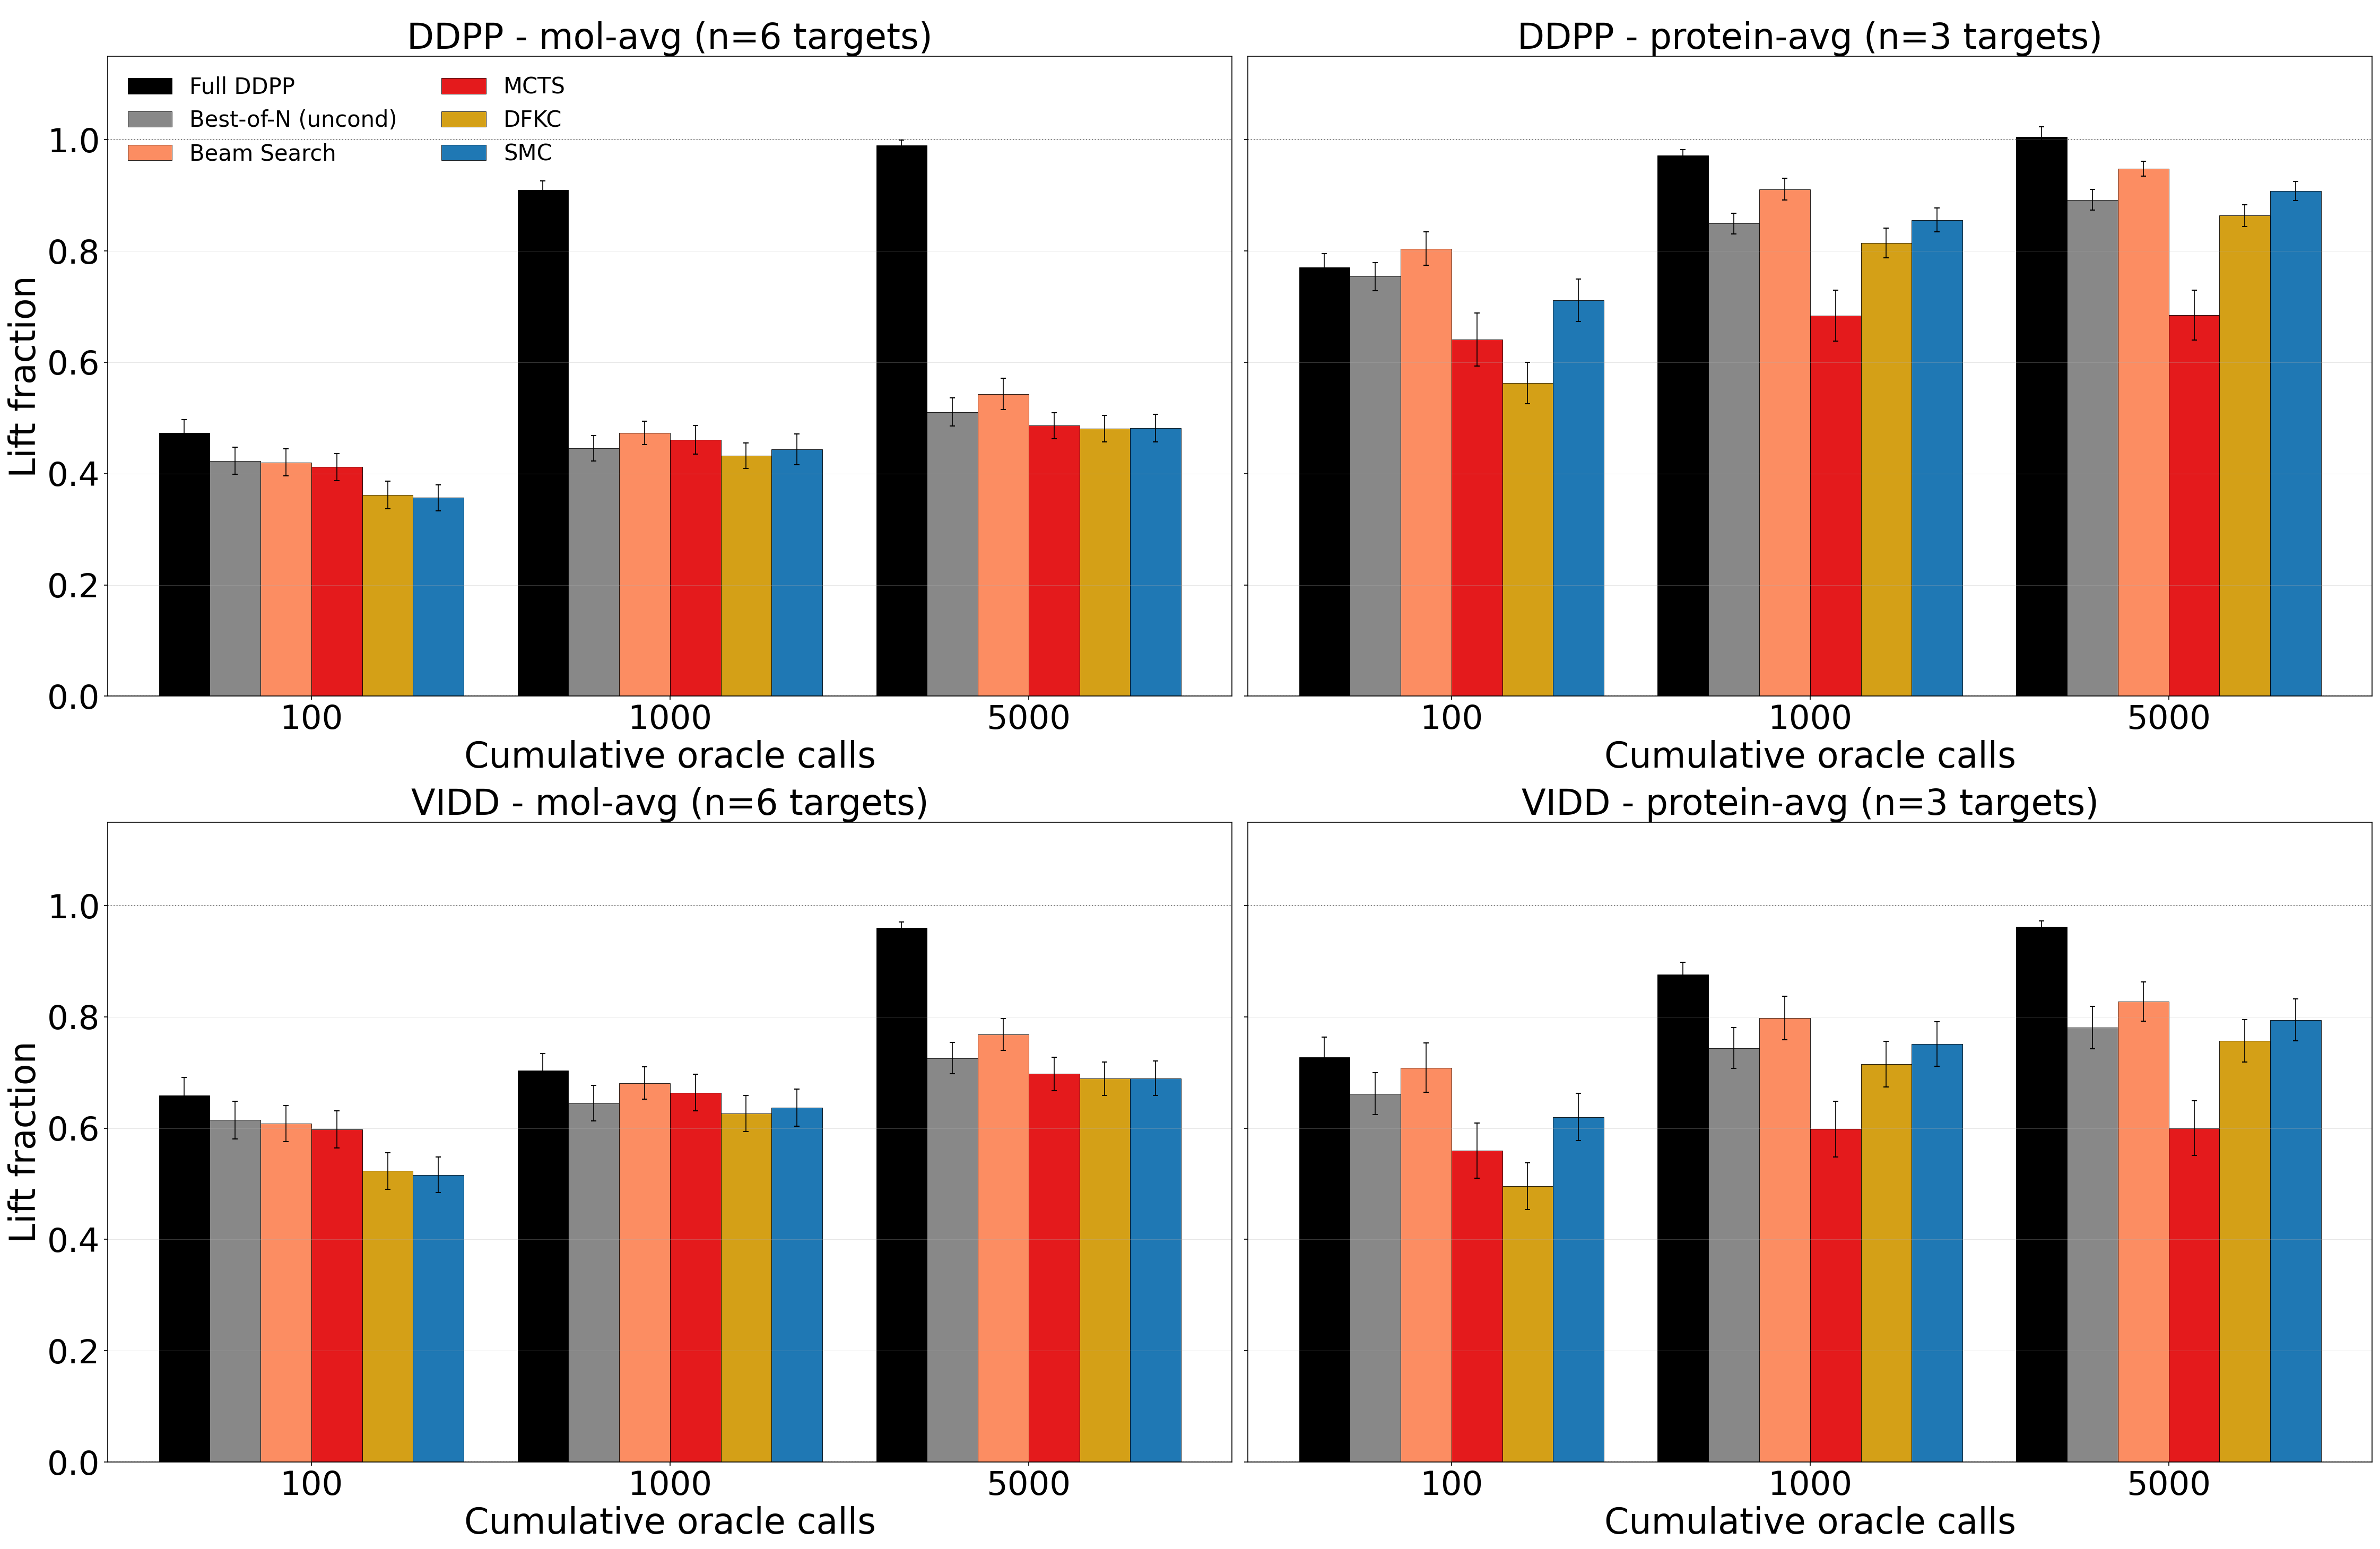
\includegraphics[width=\textwidth]{figures/ablations/result2_combined_vs_search.png}
%   \caption{\textbf{Full method vs.\ inference-time search baselines, normalised-reward bar version.} Reproduces Fig.~\ref{fig:barplot_inference_search} for appendix cross-referencing. See body for the full caption and discussion.}
% \end{figure}
% 
% 

% \section{Cross-finetuner ablation: VIDD}\label{app:vidd-ablation}

% \begin{figure}[H]
%   \centering
%   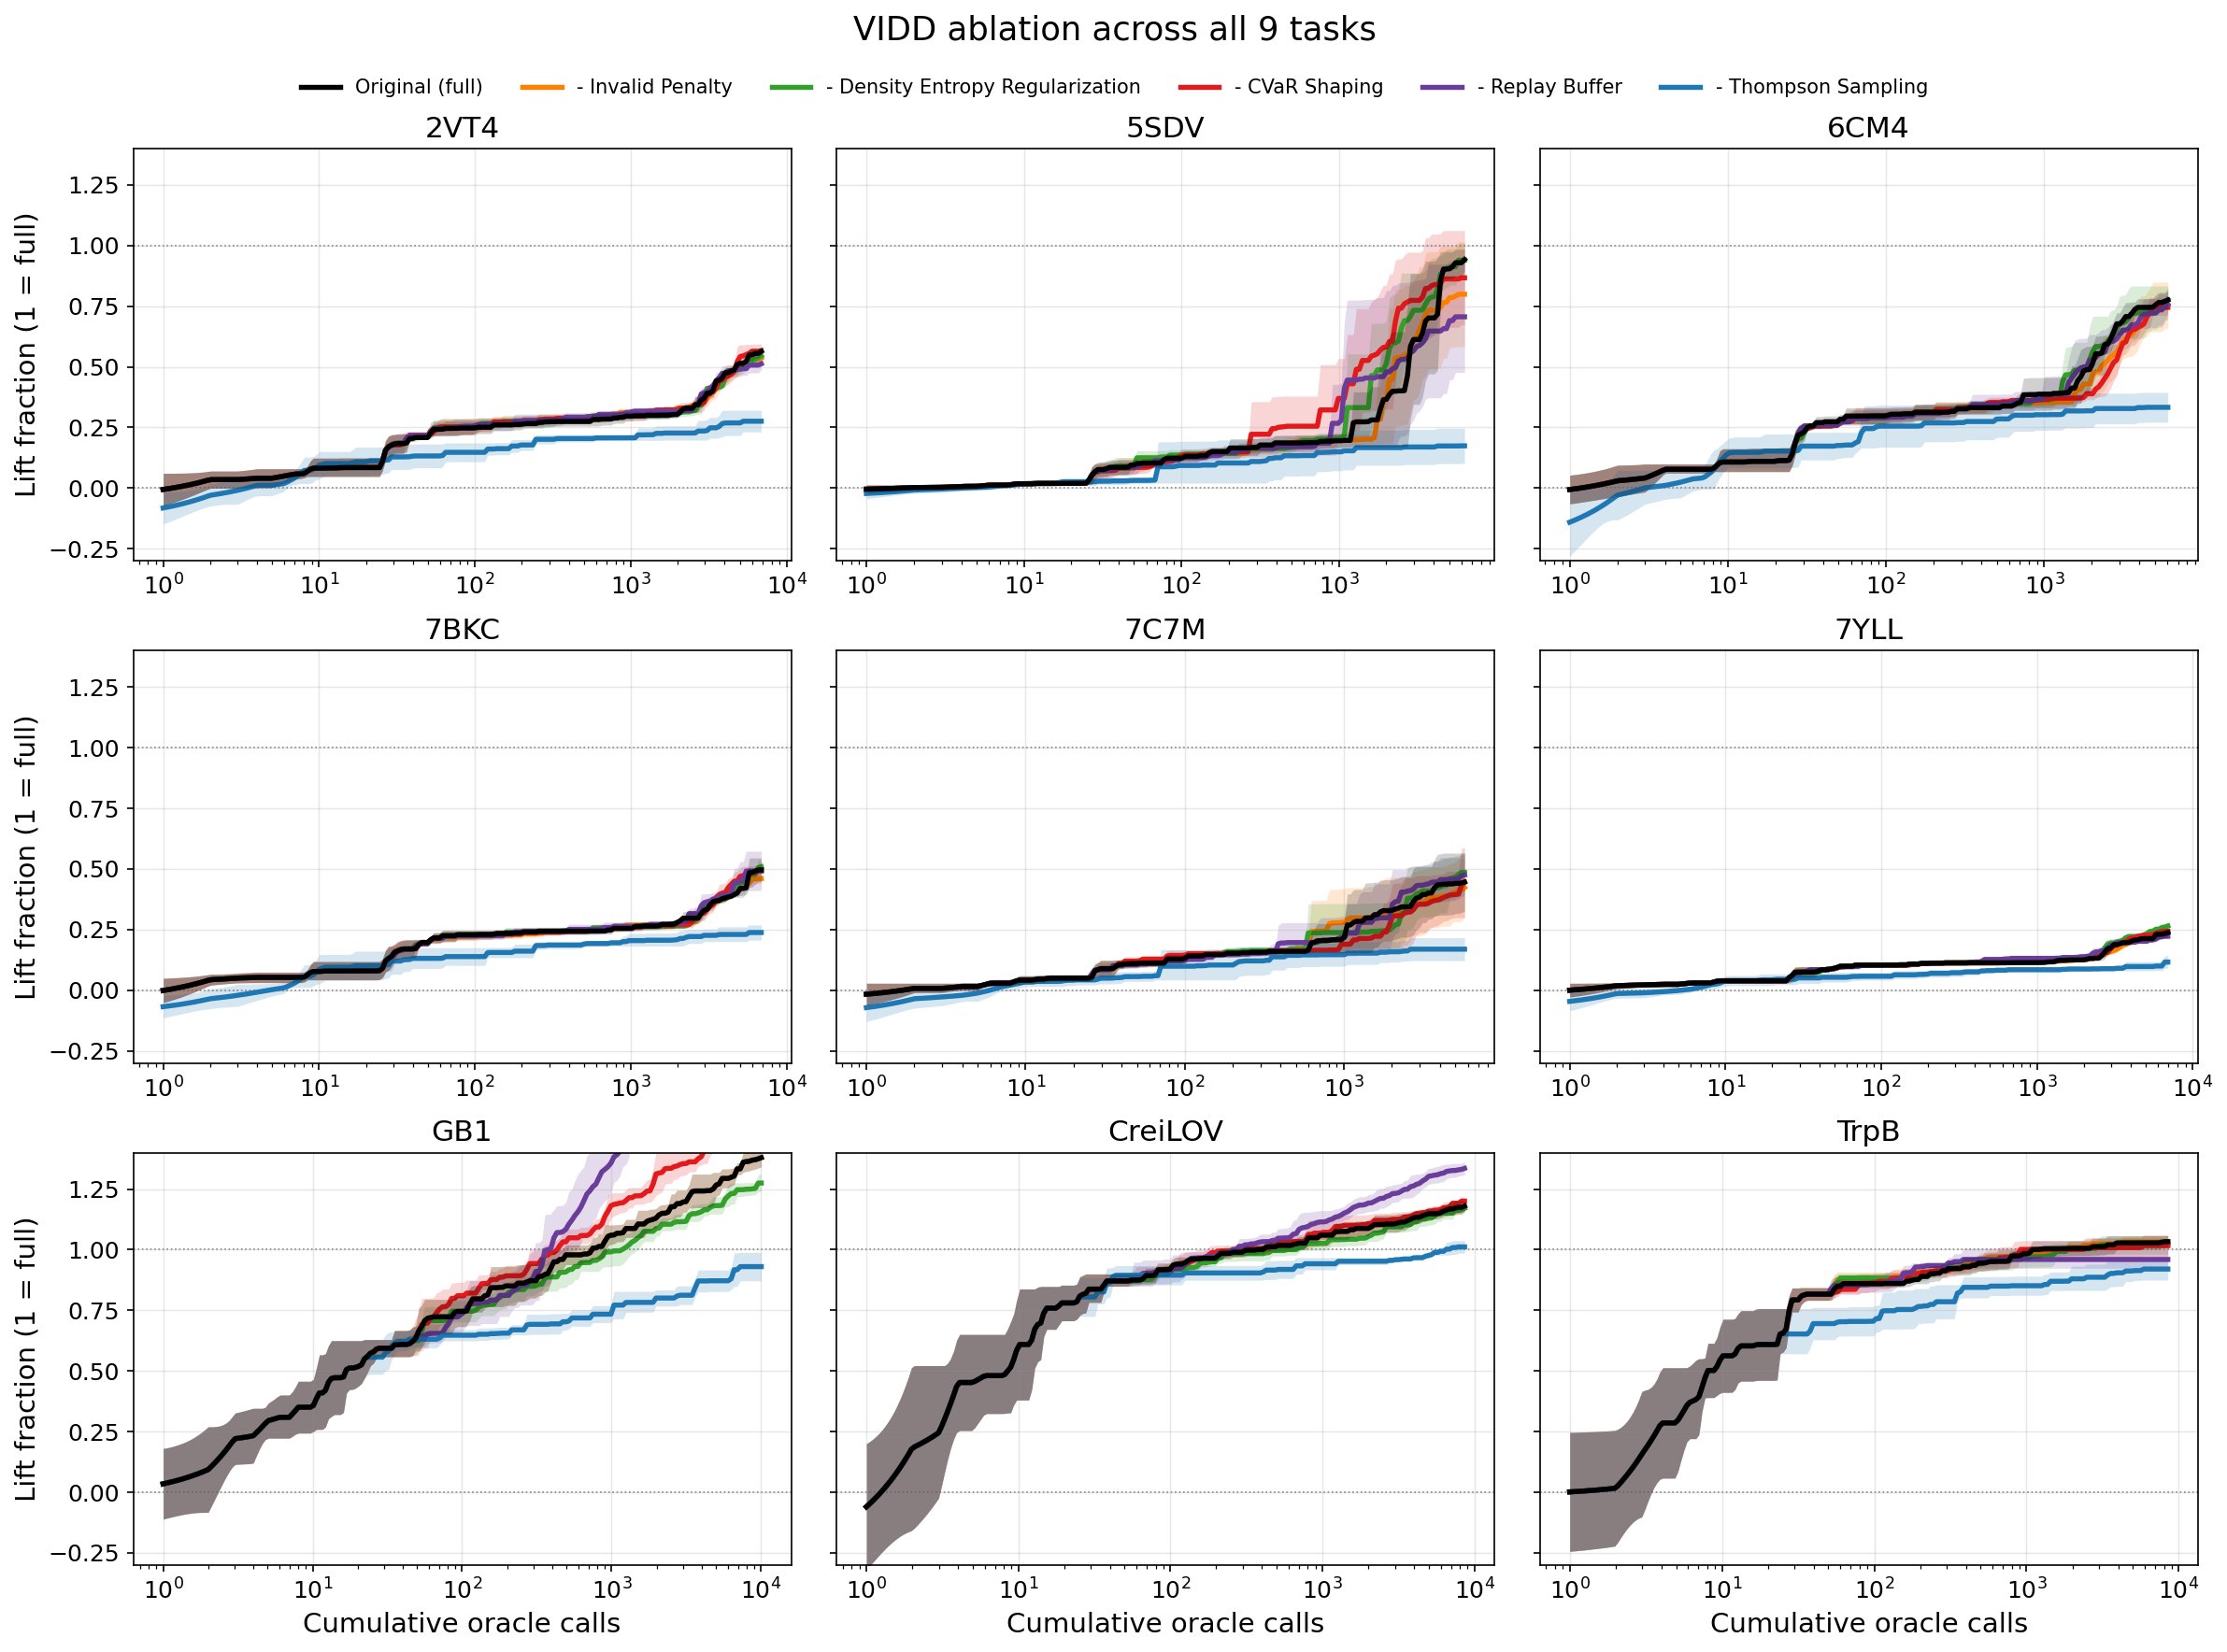
\includegraphics[width=0.95\textwidth]{figures/ablations/vidd_only_grid_norm.png}
%   \caption{\textbf{VIDD harness ablation across all $9$ tasks.} Mirror of Fig.~\ref{fig:ablation_ddpp} with VIDD substituted for DDPP-LB as the finetuning objective $\mathcal{L}_{\text{ft}}$ in the harness; lift fraction is per-target $(1 =$ full VIDD$)$. Knob ordering matches DDPP-LB on most targets, supporting the harness claim of Sec.~\ref{sec:design-space} that knob intent transfers across finetuners. Spread between ablation cells is consistently smaller under VIDD: the student-teacher distillation step damps the policy drift that the exploration / objective-mismatch knobs amplify under DDPP-LB, so each knob's marginal contribution is also damped.}
%   \label{fig:ablation_vidd}
% \end{figure}

% \section{Per-task side-by-side ablation grids}\label{app:per-task-ablation}

% The main-text figures (Fig.~\ref{fig:ablation_ddpp}, Fig.~\ref{fig:ablation_search}, and Fig.~\ref{fig:ablation_vidd} in Appendix~\ref{app:vidd-ablation}) hold the finetuner / search-family fixed and step through the $9$ tasks. The figures below transpose that view: each $3 \times 3$ grid groups rows by task and places DDPP-LB, VIDD, and search-only baselines side by side per task. Same normalised-reward definition and conventions as Sec.~\ref{sec:exp-setup}.

% \begin{figure}[H]
%   \centering
%   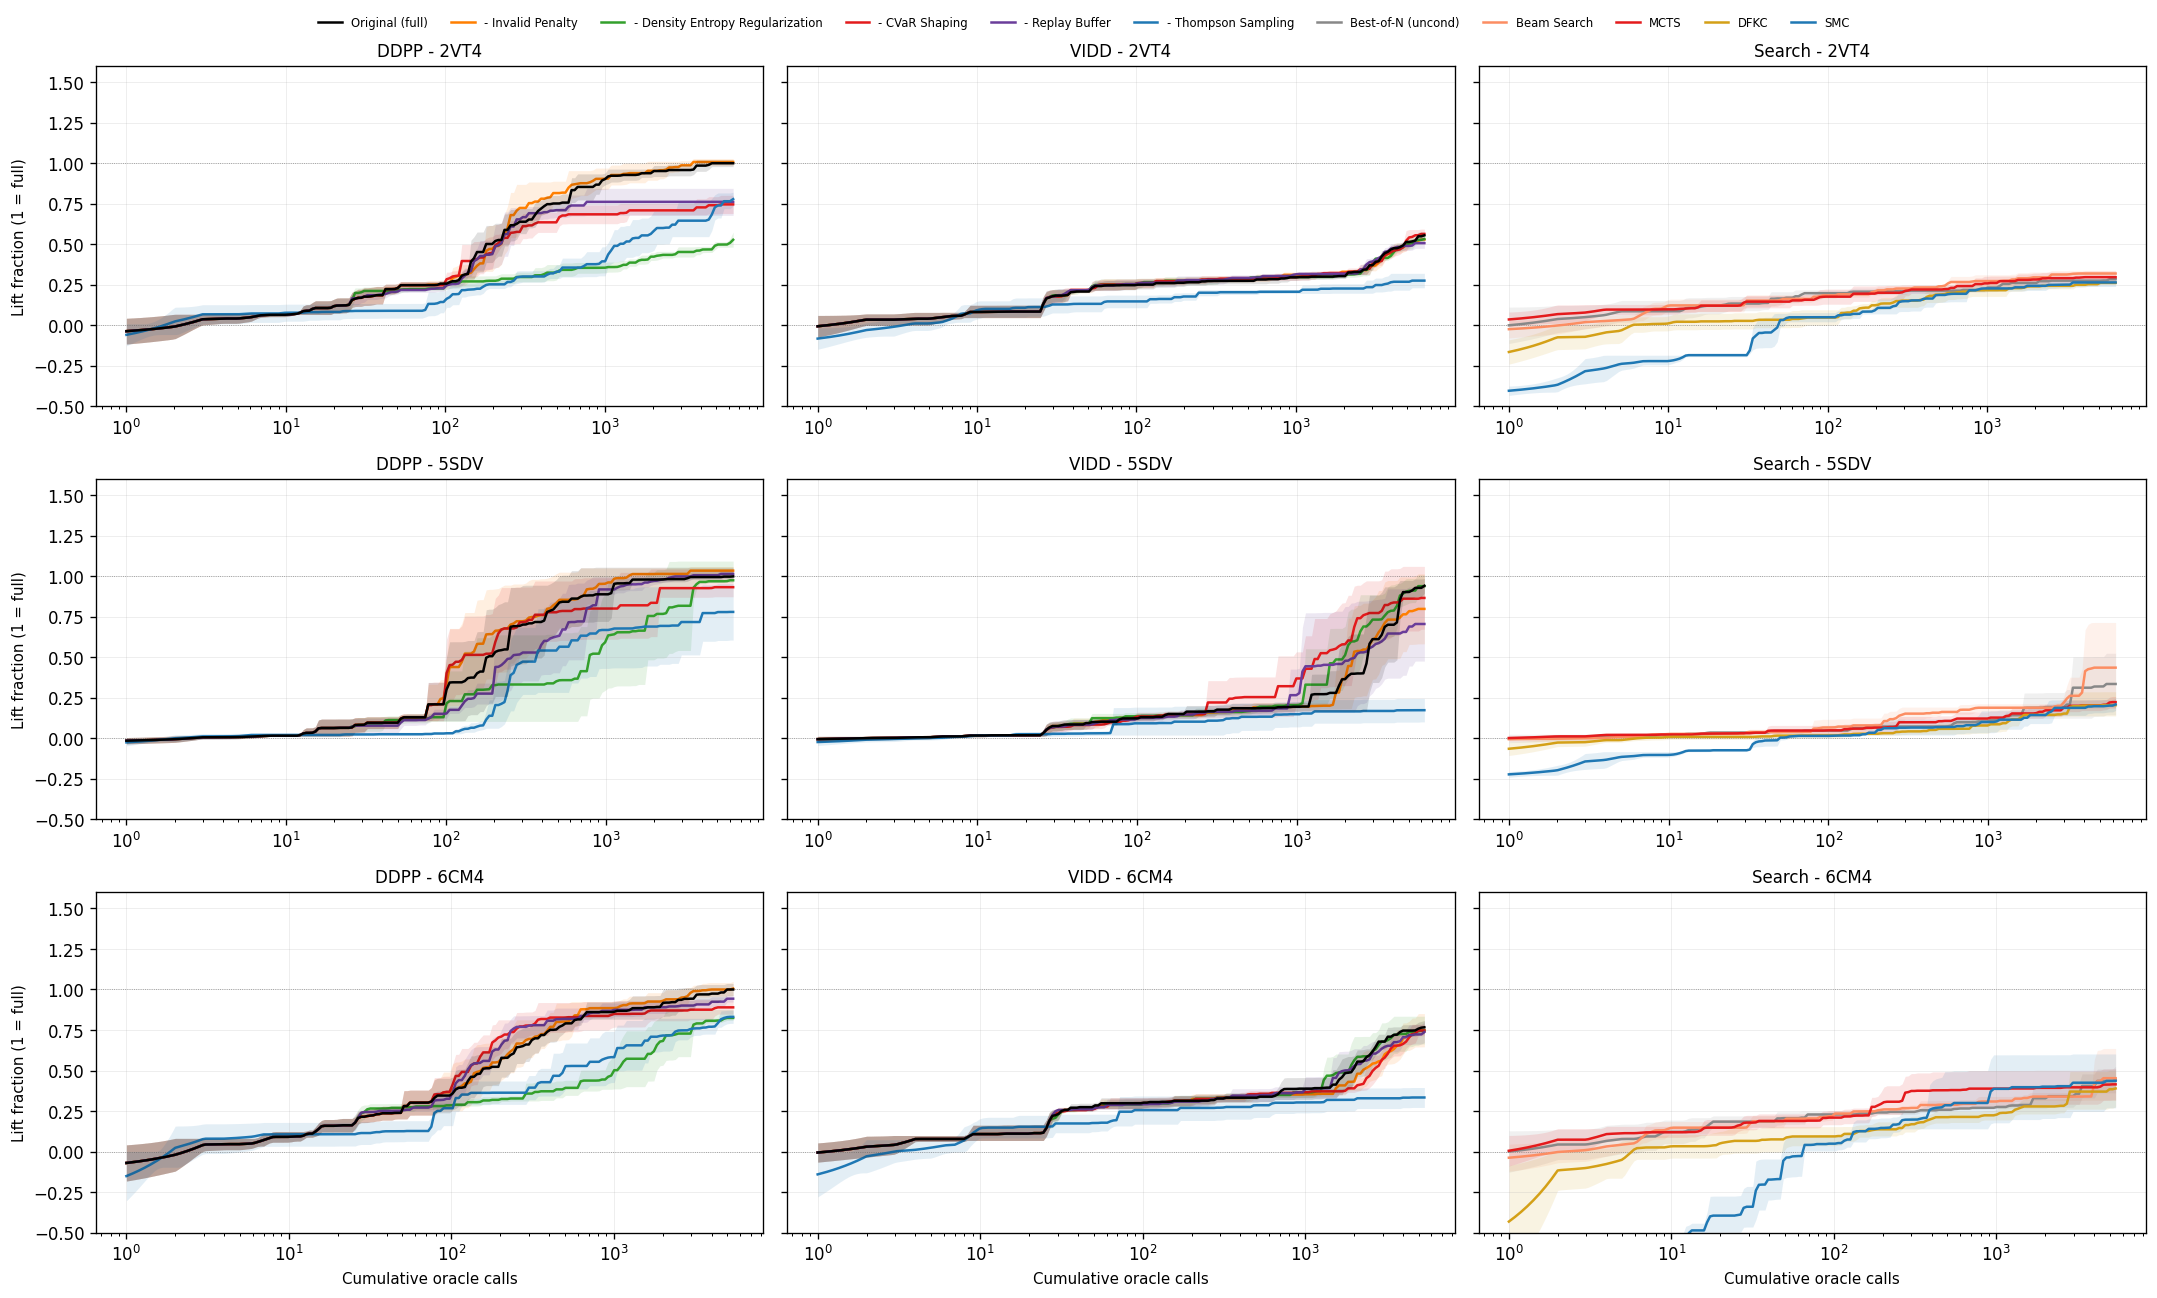
\includegraphics[width=0.95\textwidth]{figures/ablations/mol_ablations_grid_set1_norm.png}
%   \caption{\textbf{Per-task ablation, small molecules (set 1: 2VT4, 5SDV, 6CM4).} Rows are FA-oracle targets; columns are DDPP-LB ablations (left), VIDD ablations (centre), search baselines (right). The VIDD column is consistently more compressed than DDPP-LB on the same target, matching the cross-finetuner observation in Fig.~\ref{fig:ablation_vidd}.}
%   \label{fig:per_task_mol_set1}
% \end{figure}

% \begin{figure}[H]
%   \centering
%   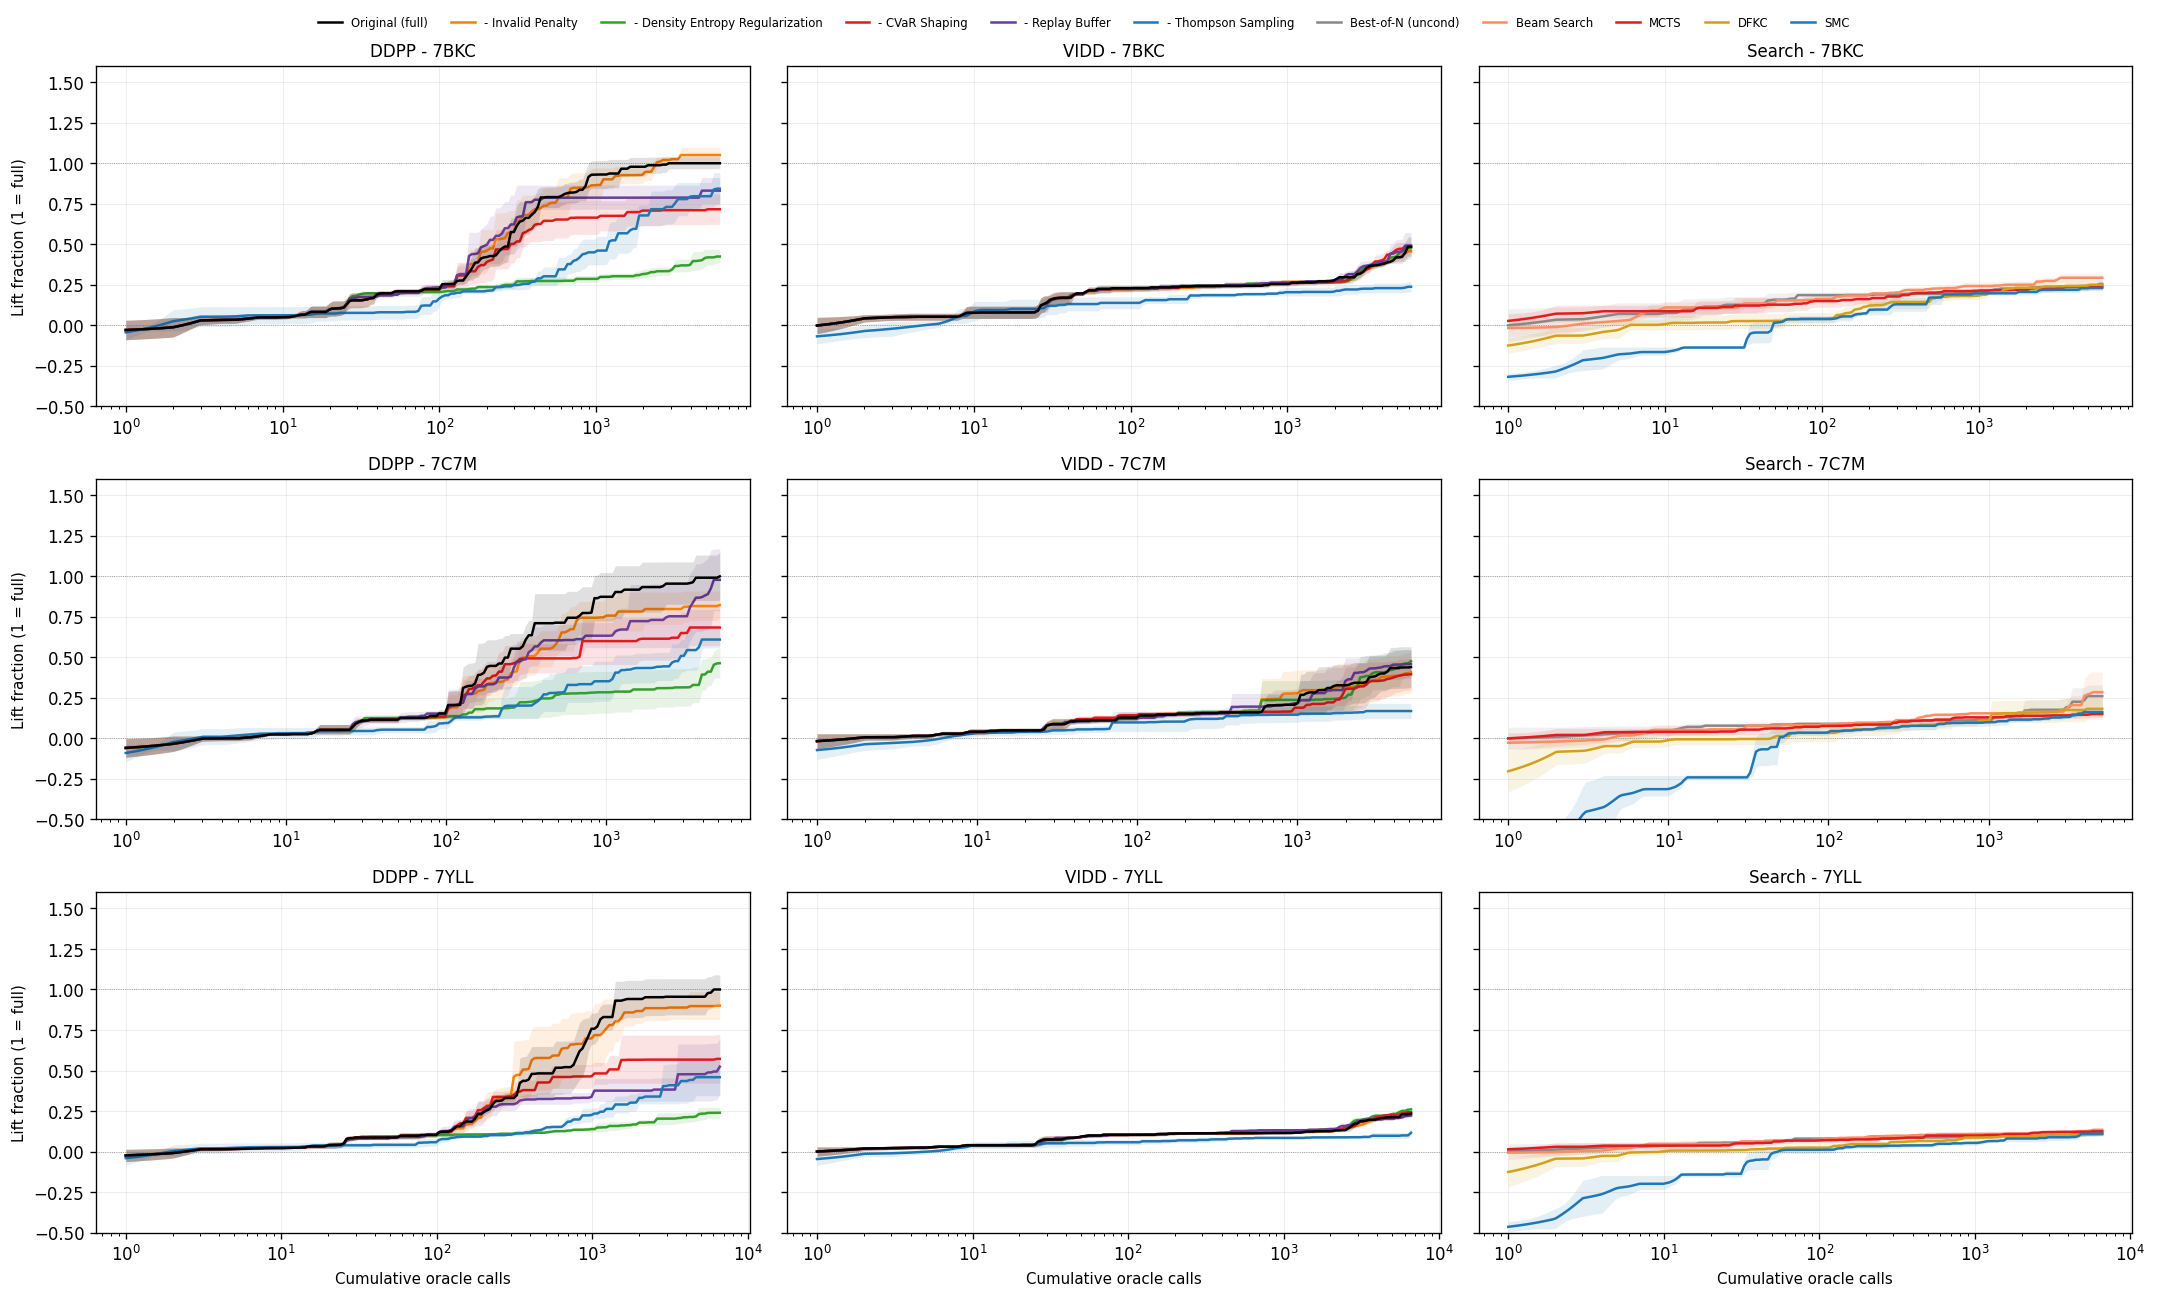
\includegraphics[width=0.95\textwidth]{figures/ablations/mol_ablations_grid_set2_norm.png}
%   \caption{\textbf{Per-task ablation, small molecules (set 2: 7BKC, 7C7M, 7YLL).} Continuation of Fig.~\ref{fig:per_task_mol_set1} for the remaining three FA-oracle targets. The 7C7M row is extreme: removing \textit{- Density Entropy Regularization} drops DDPP-LB to a small fraction of the full method, while the same removal under VIDD has a much smaller effect --- consistent with the student-teacher damping of policy drift discussed in Appendix~\ref{app:vidd-ablation}.}
%   \label{fig:per_task_mol_set2}
% \end{figure}

% \begin{figure}[H]
%   \centering
%   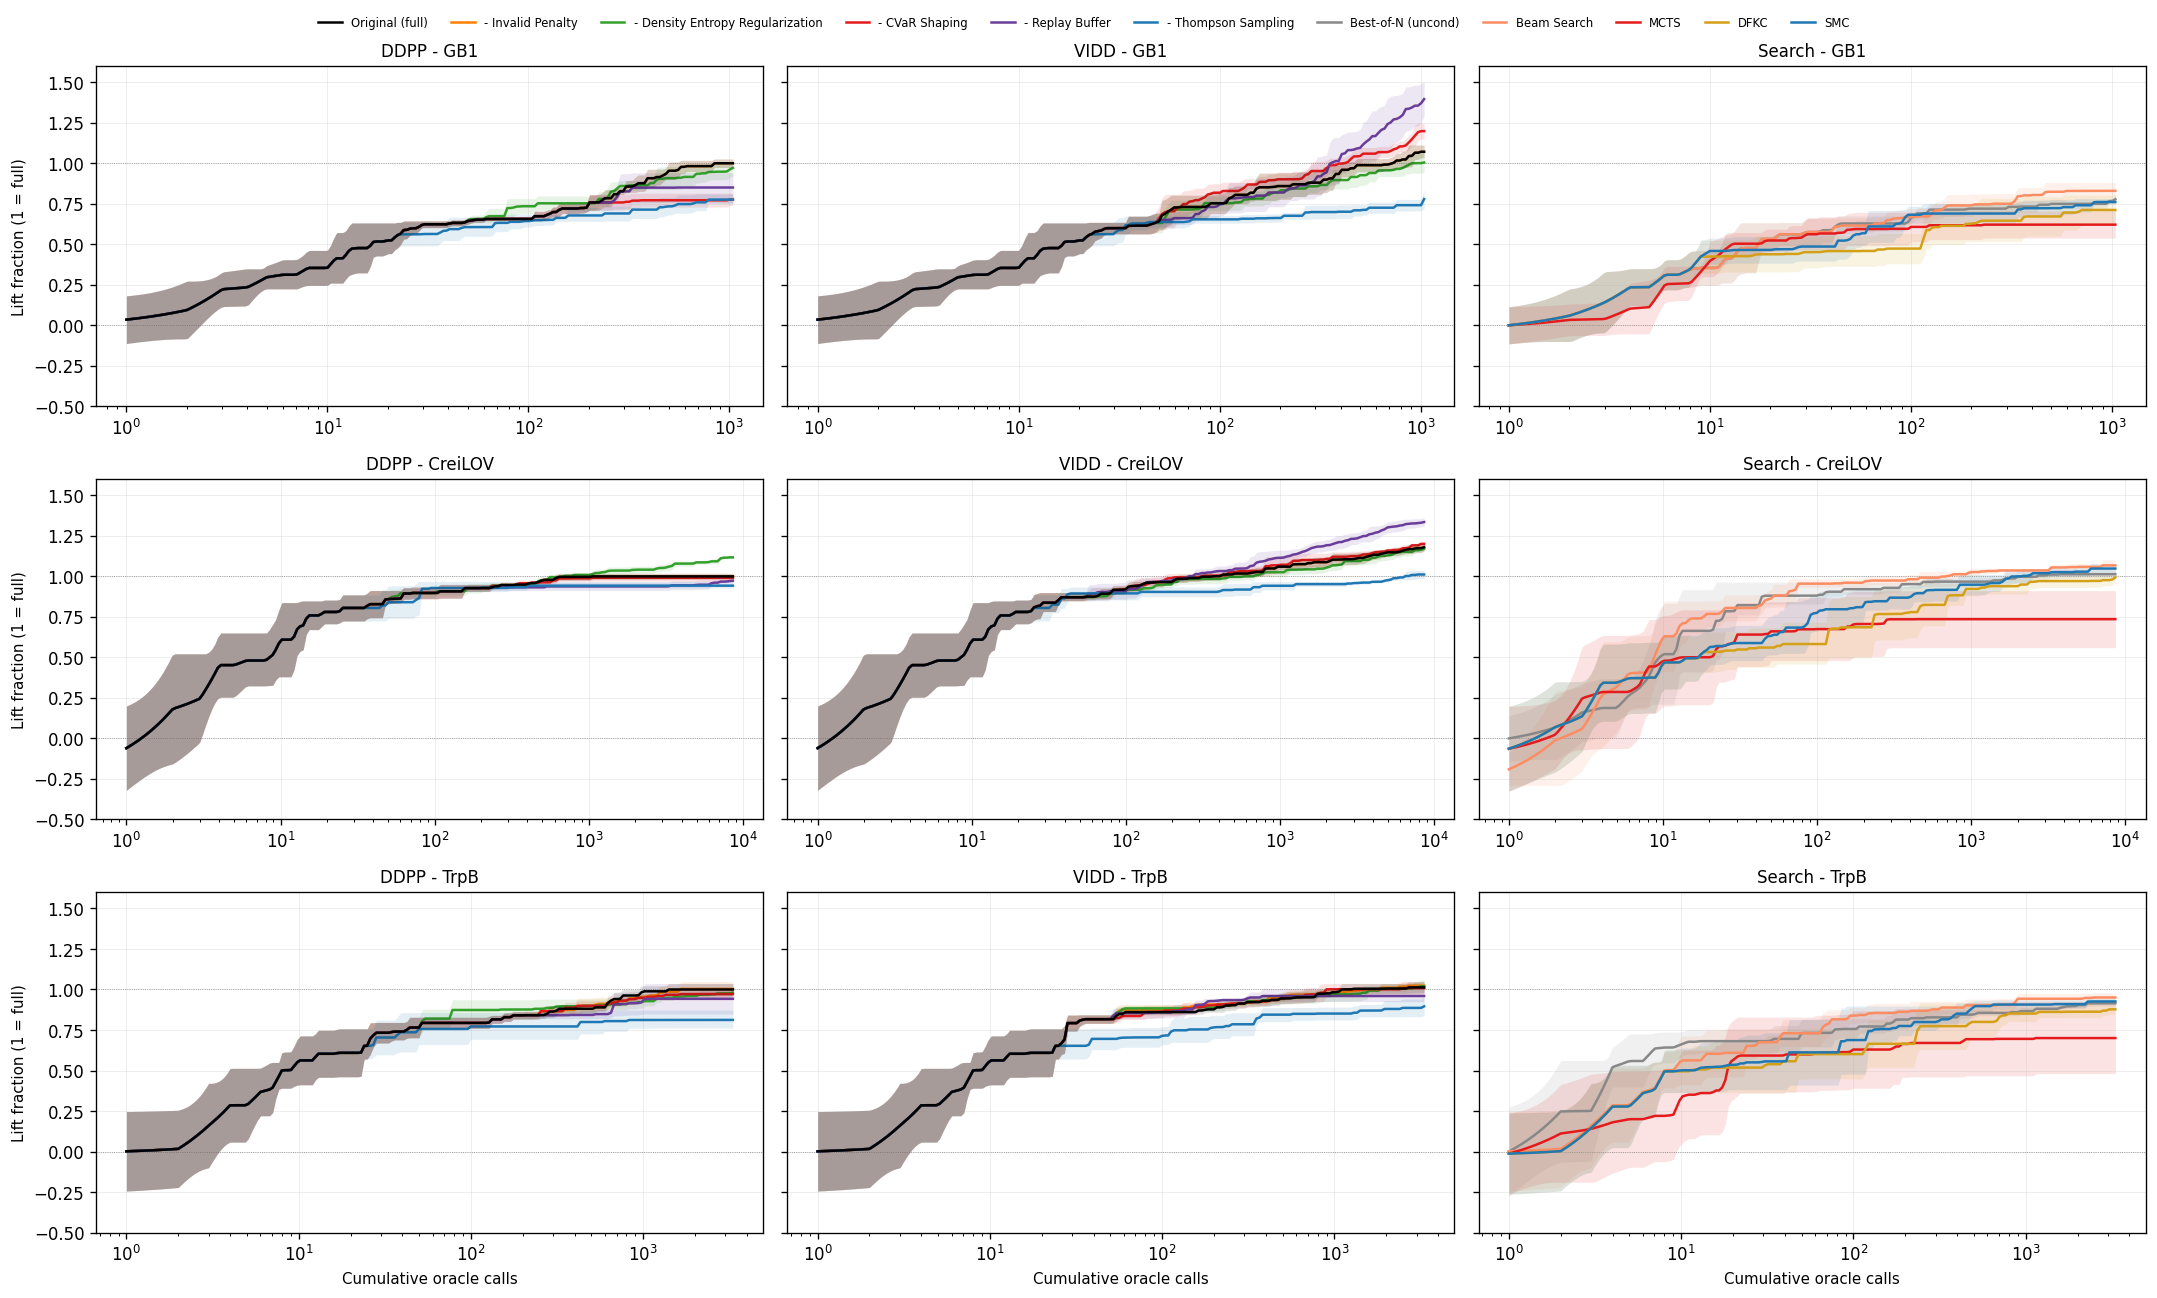
\includegraphics[width=0.95\textwidth]{figures/ablations/protein_ablations_grid_norm.png}
%   \caption{\textbf{Per-task ablation, protein-fitness targets (GB1, CreiLOV, TrpB).} Rows are protein-fitness families; columns match Fig.~\ref{fig:per_task_mol_set1}. CI bands are wider than the small-molecule rows because each family has a single trained surrogate / generator pair (no within-family pooling).}
%   \label{fig:per_task_protein}
% \end{figure}

% \section{Aggregated ablation grids}\label{app:avg-ablation}

% The per-task figures above retain the cross-target spread that motivates the manifold / mode-density discussion in Sec.~\ref{sec:results}. The figures below collapse that spread by averaging the normalised-reward curves across the $6$ FA-oracle small molecules (top row) and across the $3$ protein-fitness families (bottom row), giving a single curve per knob per axis-type. CI bands are across-target ($\pm 1.96 \cdot \mathrm{SEM}$), so they reflect target-level rather than seed-level variability.

% \begin{figure}[H]
%   \centering
%   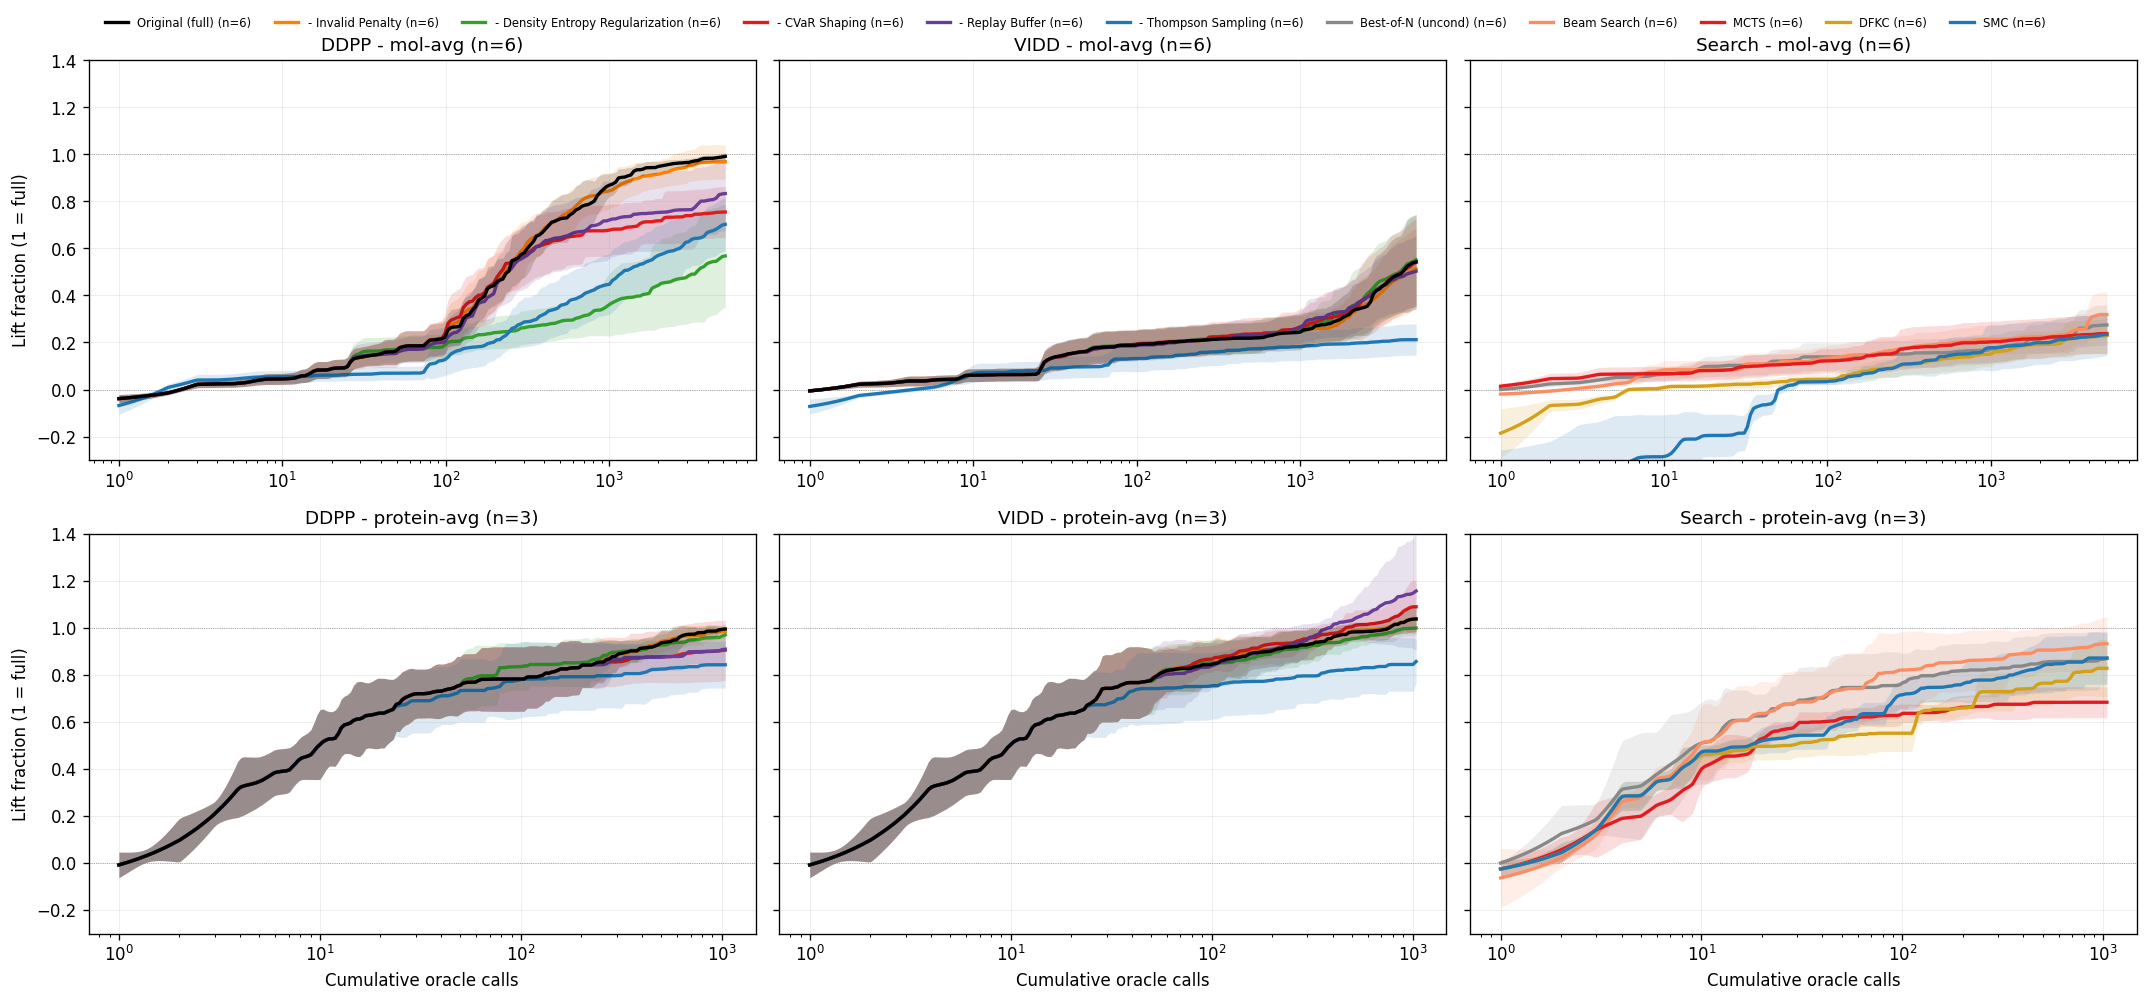
\includegraphics[width=0.95\textwidth]{figures/ablations/avg_grid_norm.png}
%   \caption{\textbf{Aggregated ablation grid, oracle-call view.} $2 \times 3$ grid: row $1$ averages over all six FA-oracle small molecules, row $2$ averages over the three protein-fitness families; columns are DDPP-LB ablations, VIDD ablations, and search-only baselines. Same normalised-reward definition as Fig.~\ref{fig:ablation_ddpp}. Across-target CI bands (target-level variability) are wider than the per-target seed bands in the figures above.}
%   \label{fig:avg_ablation_calls}
% \end{figure}

% \begin{figure}[H]
%   \centering
%   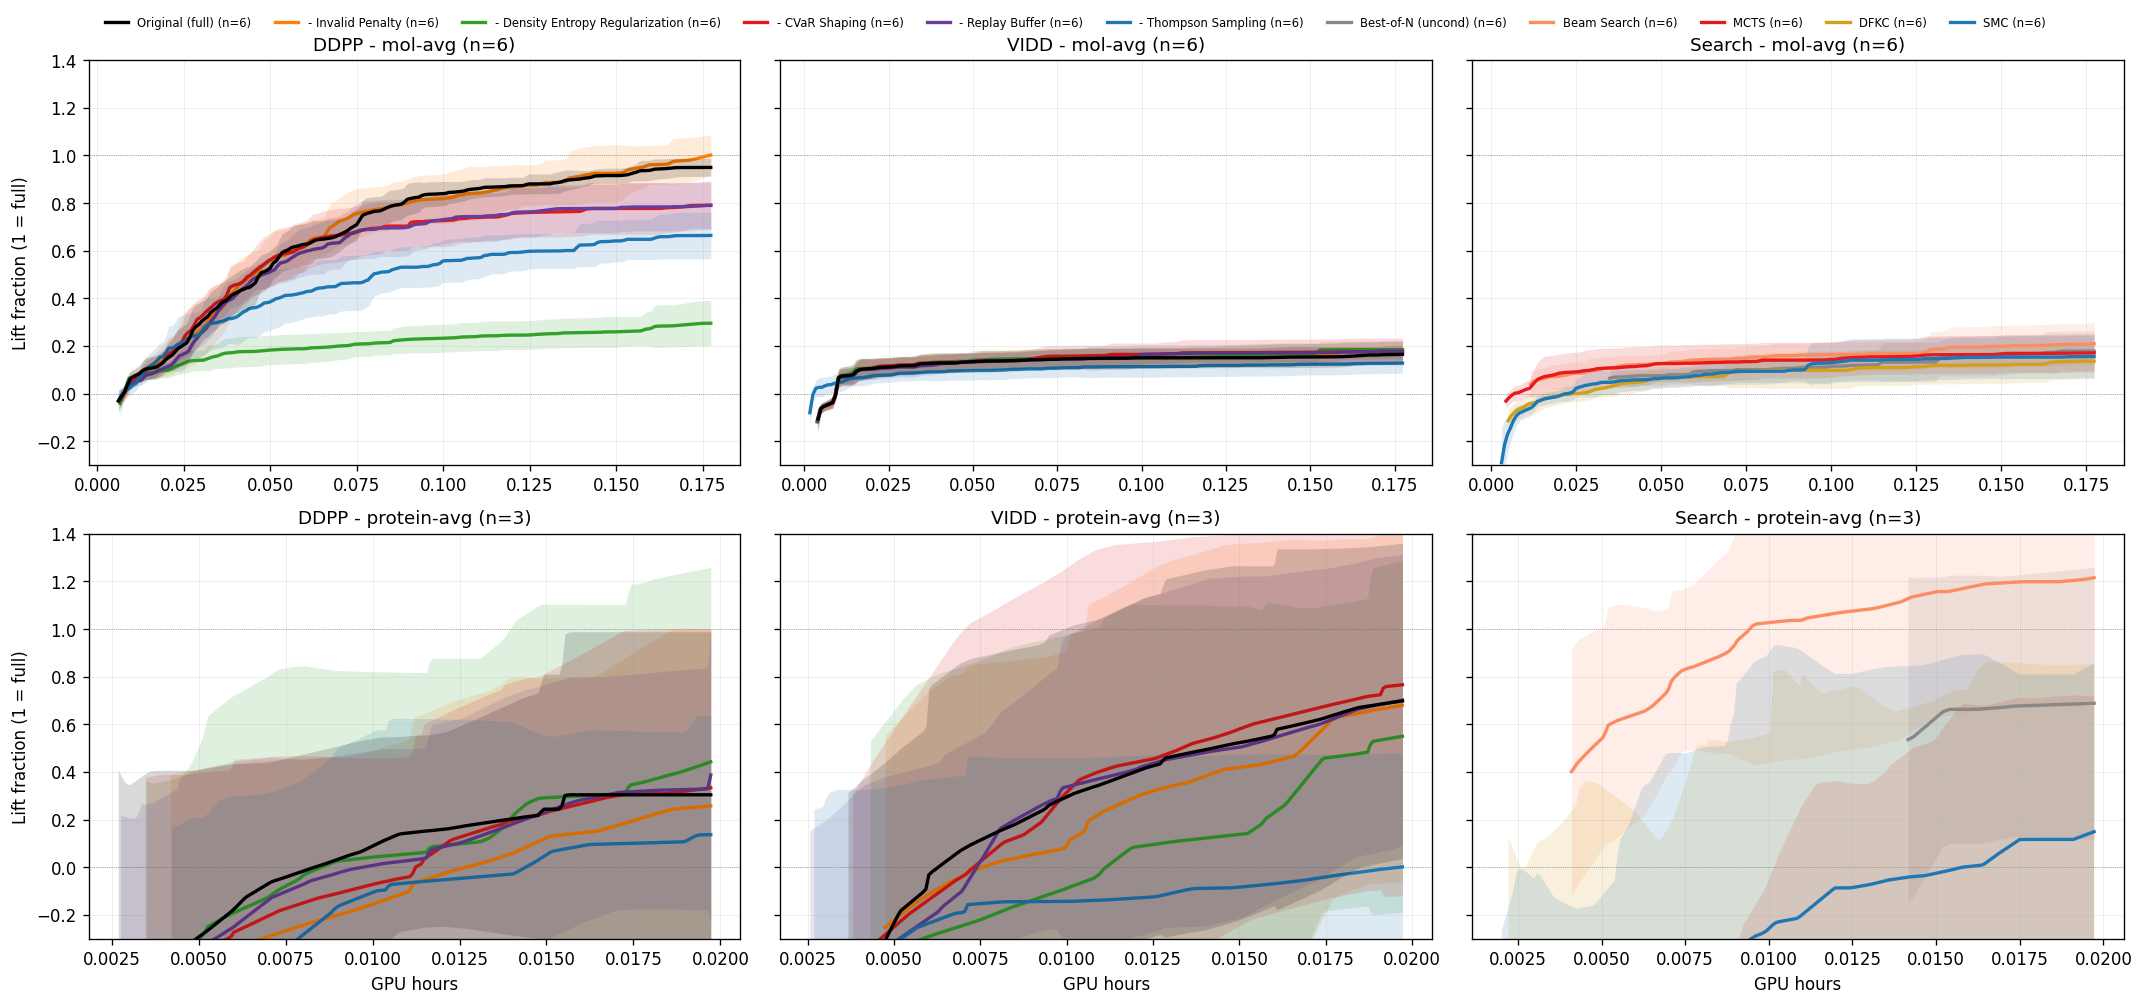
\includegraphics[width=0.95\textwidth]{figures/ablations/avg_grid_norm_gpuhrs.png}
%   \caption{\textbf{Aggregated ablation grid, GPU-hours view.} GPU-hours twin of Fig.~\ref{fig:avg_ablation_calls}; same averaging.}
%   \label{fig:avg_ablation_gpuhrs}
% \end{figure}

% \section{GPU-hour view of the ablation grids}\label{app:gpuhrs-ablation}

% The main-text and per-task ablation grids (Figs.~\ref{fig:ablation_ddpp}, \ref{fig:ablation_search}, \ref{fig:ablation_vidd}, \ref{fig:per_task_mol_set1}, \ref{fig:per_task_mol_set2}, \ref{fig:per_task_protein}) use cumulative oracle calls on the x-axis to isolate feedback efficiency. This appendix replots the same data against GPU hours, including method-side cost (generation, scoring, surrogate update, finetuning); see Sec.~\ref{sec:exp-setup} for the motivation. Same normalised-reward definition throughout.

% \begin{figure}[H]
%   \centering
%   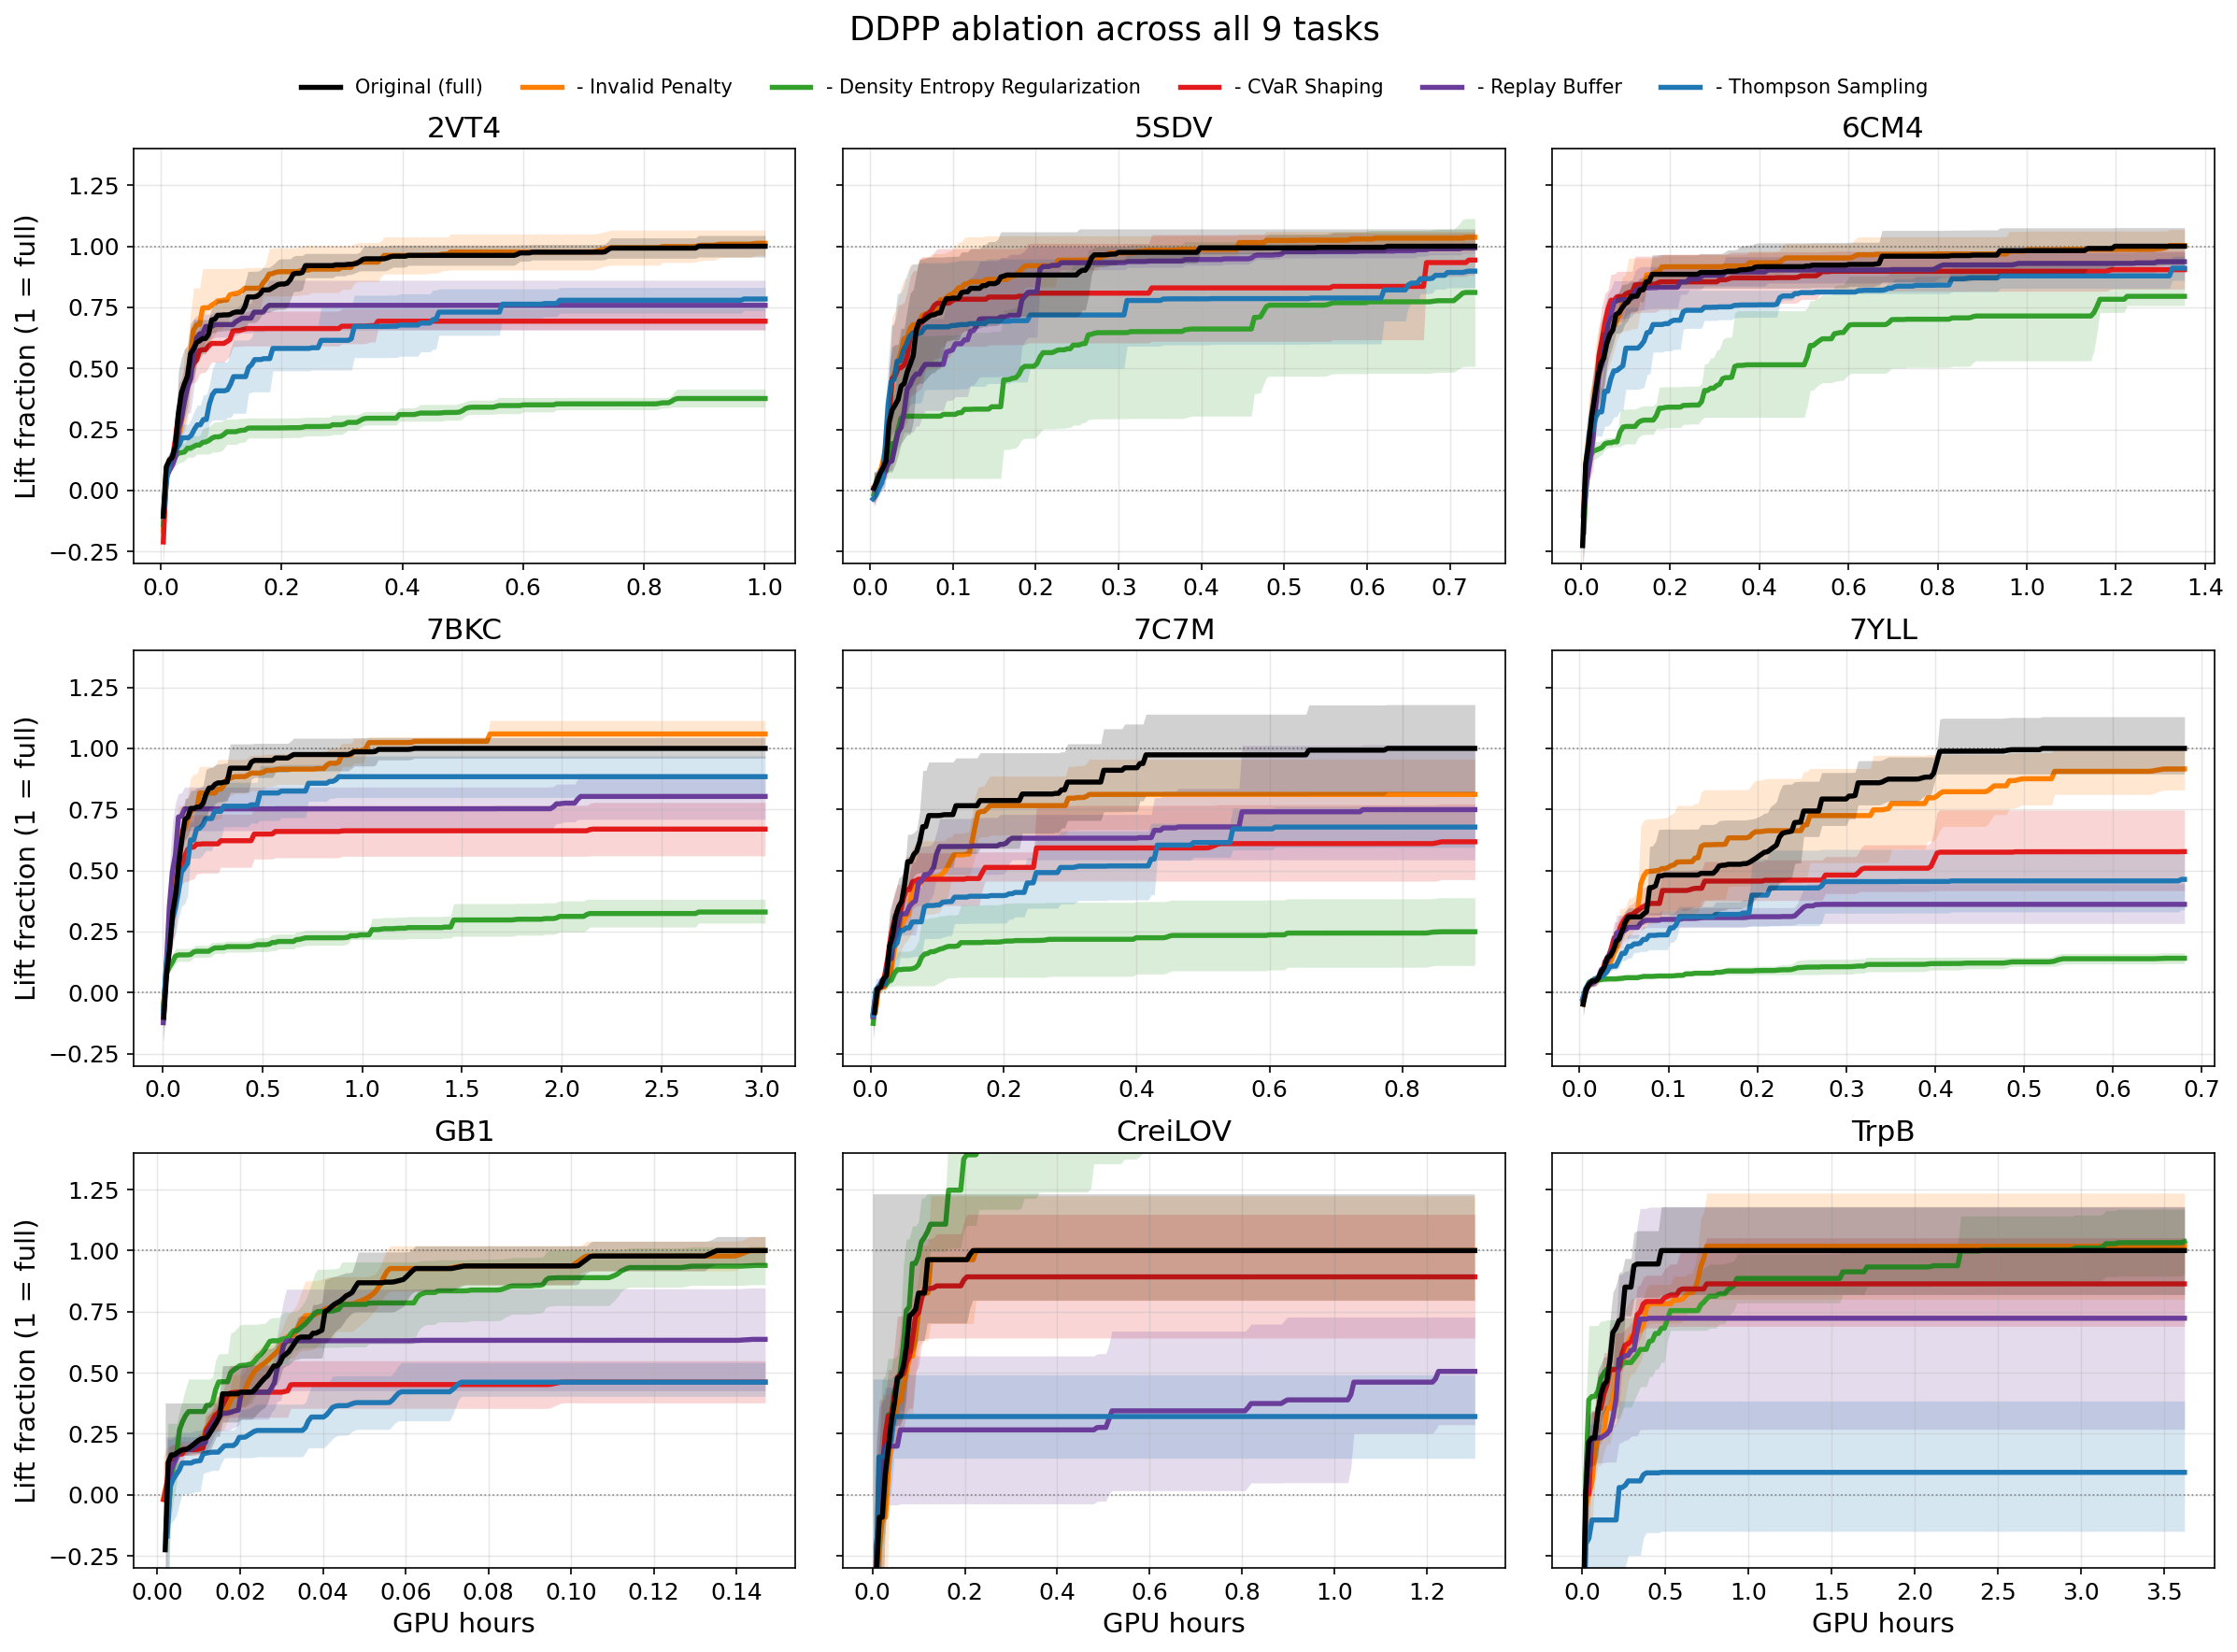
\includegraphics[width=0.95\textwidth]{figures/ablations/ddpp_only_grid_norm_gpuhrs.png}
%   \caption{\textbf{DDPP-LB harness ablation, GPU-hours view.} GPU-hours twin of Fig.~\ref{fig:ablation_ddpp}. Knob ordering is largely preserved, but the gap between the full method and \textit{- Thompson sampling} narrows in wall time --- the Thompson step adds non-trivial method-side cost.}
%   \label{fig:ablation_ddpp_gpuhrs}
% \end{figure}

% \begin{figure}[H]
%   \centering
%   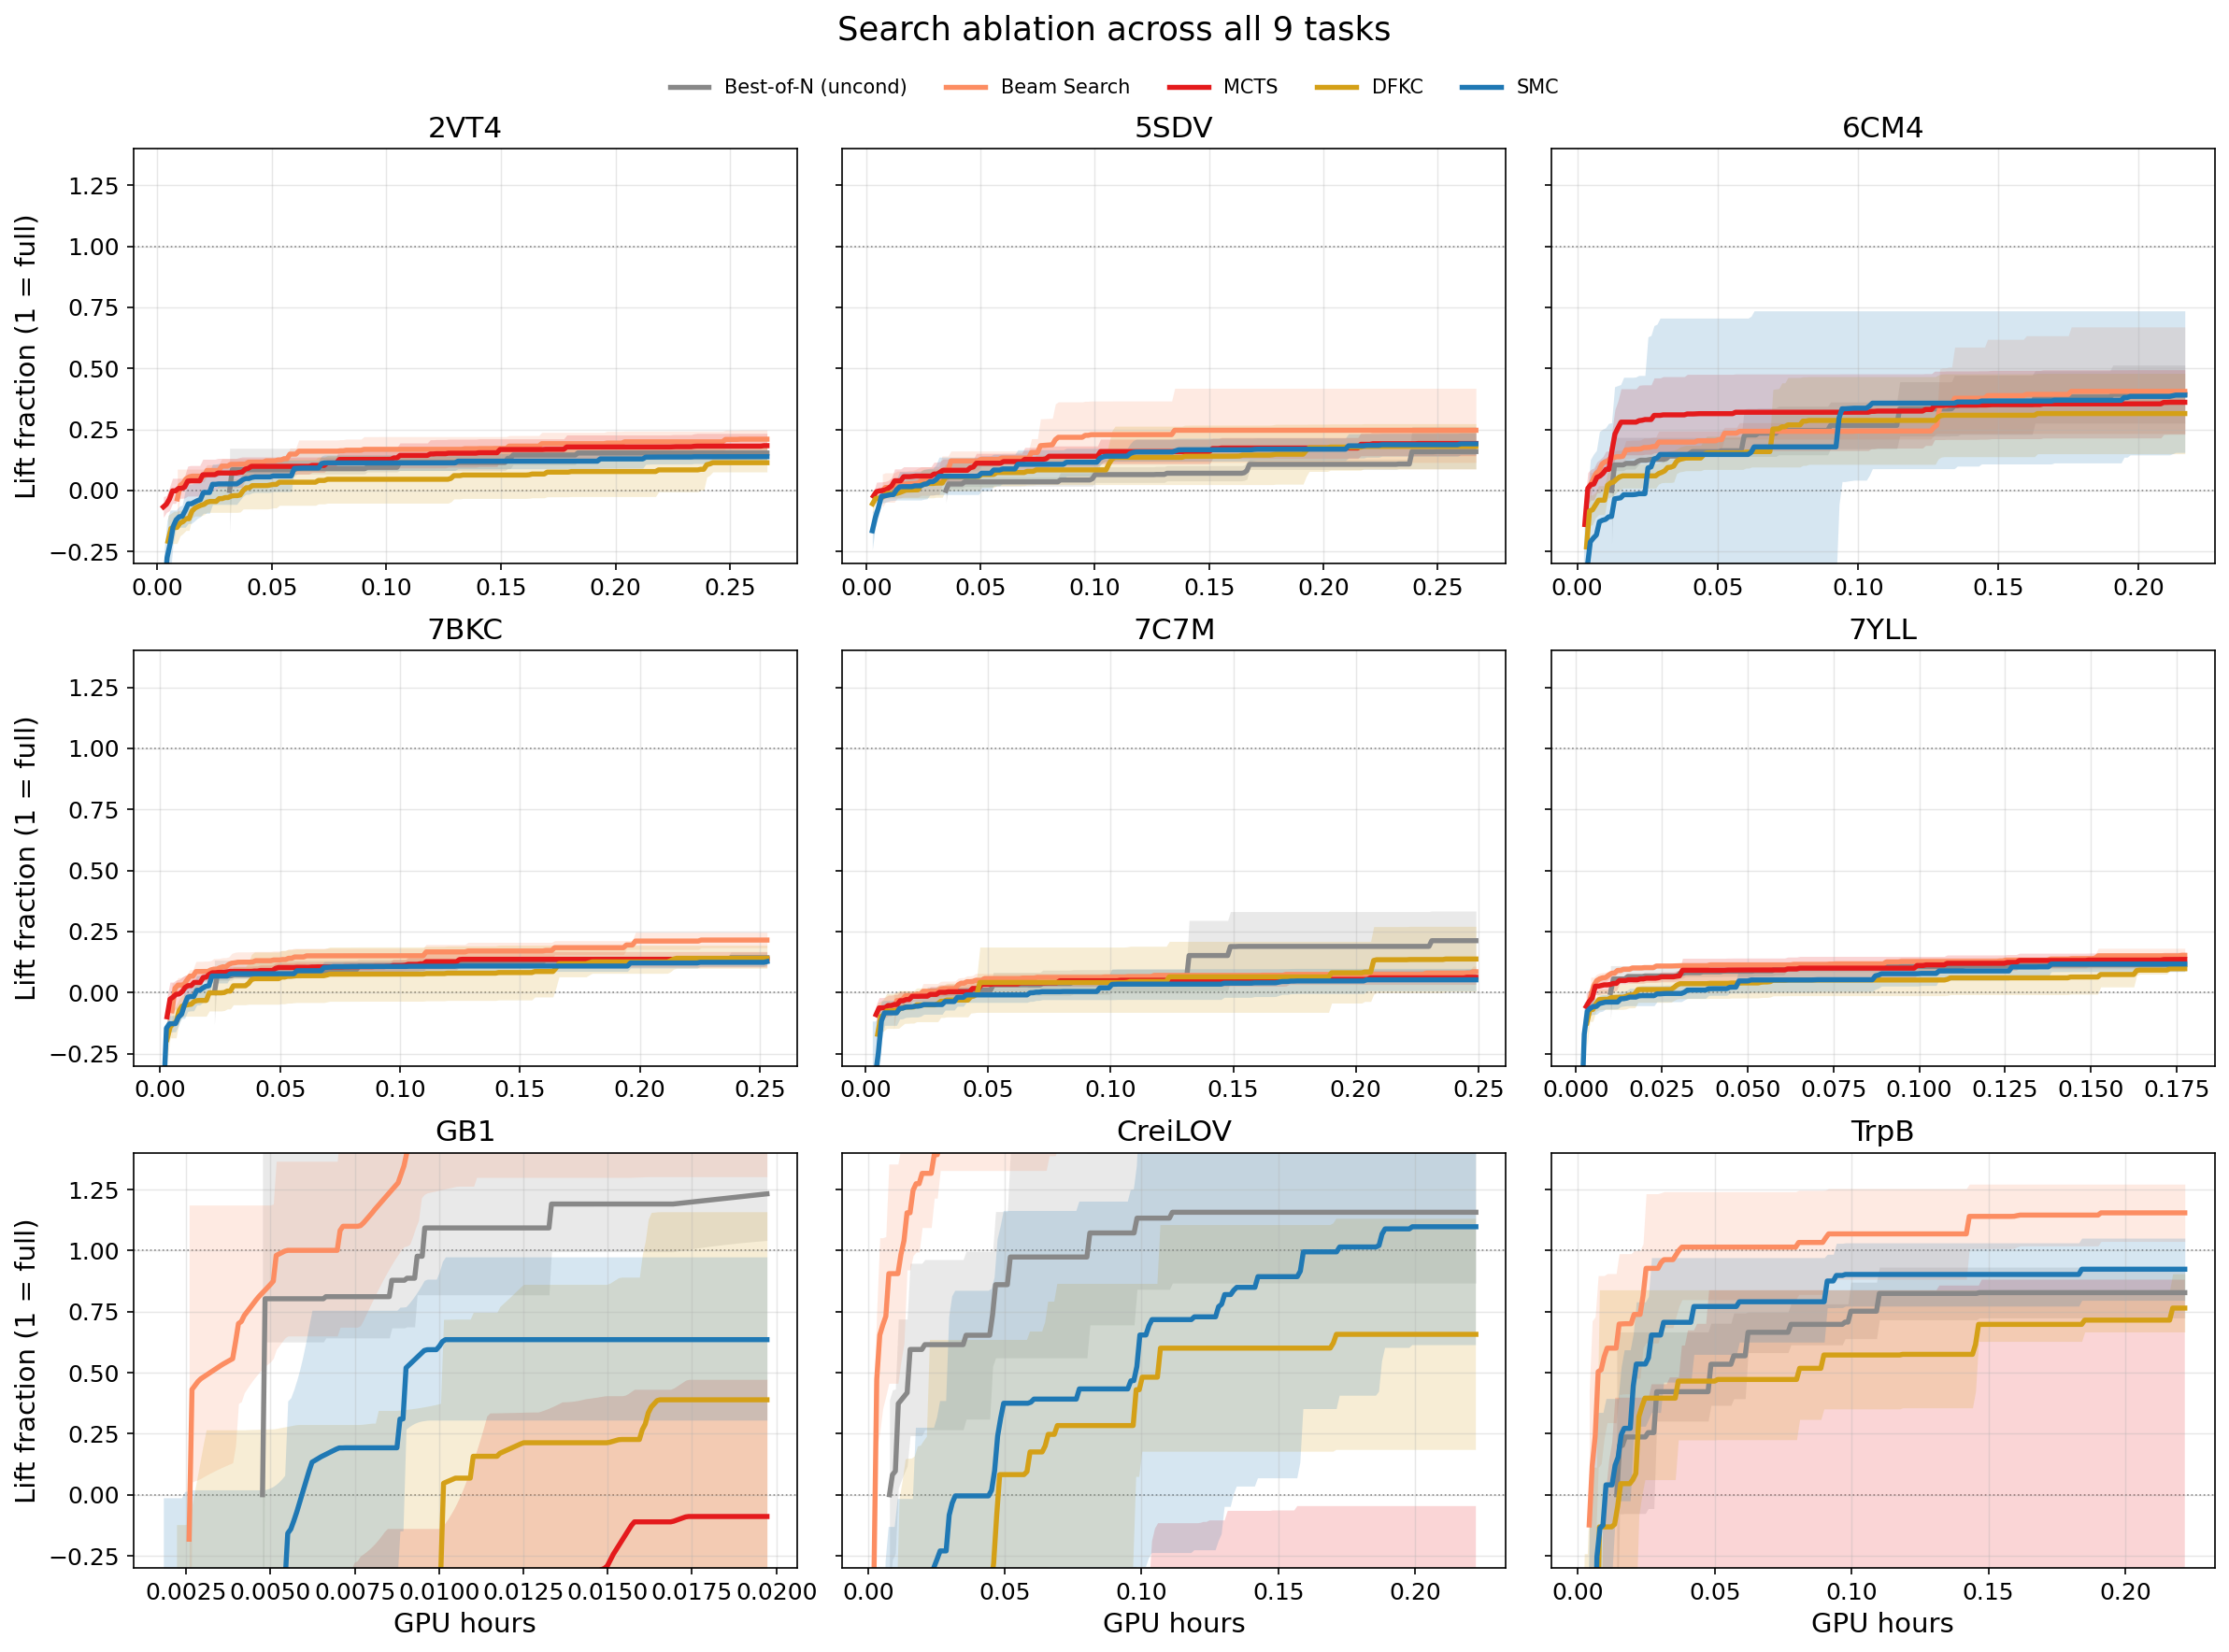
\includegraphics[width=0.95\textwidth]{figures/ablations/search_only_grid_norm_gpuhrs.png}
%   \caption{\textbf{Search-only baselines, GPU-hours view.} GPU-hours twin of Fig.~\ref{fig:ablation_search}. Plain best-of-$N$ wins on wall time more often than on oracle-call efficiency --- no per-call surrogate / search overhead.}
%   \label{fig:ablation_search_gpuhrs}
% \end{figure}

% \begin{figure}[H]
%   \centering
%   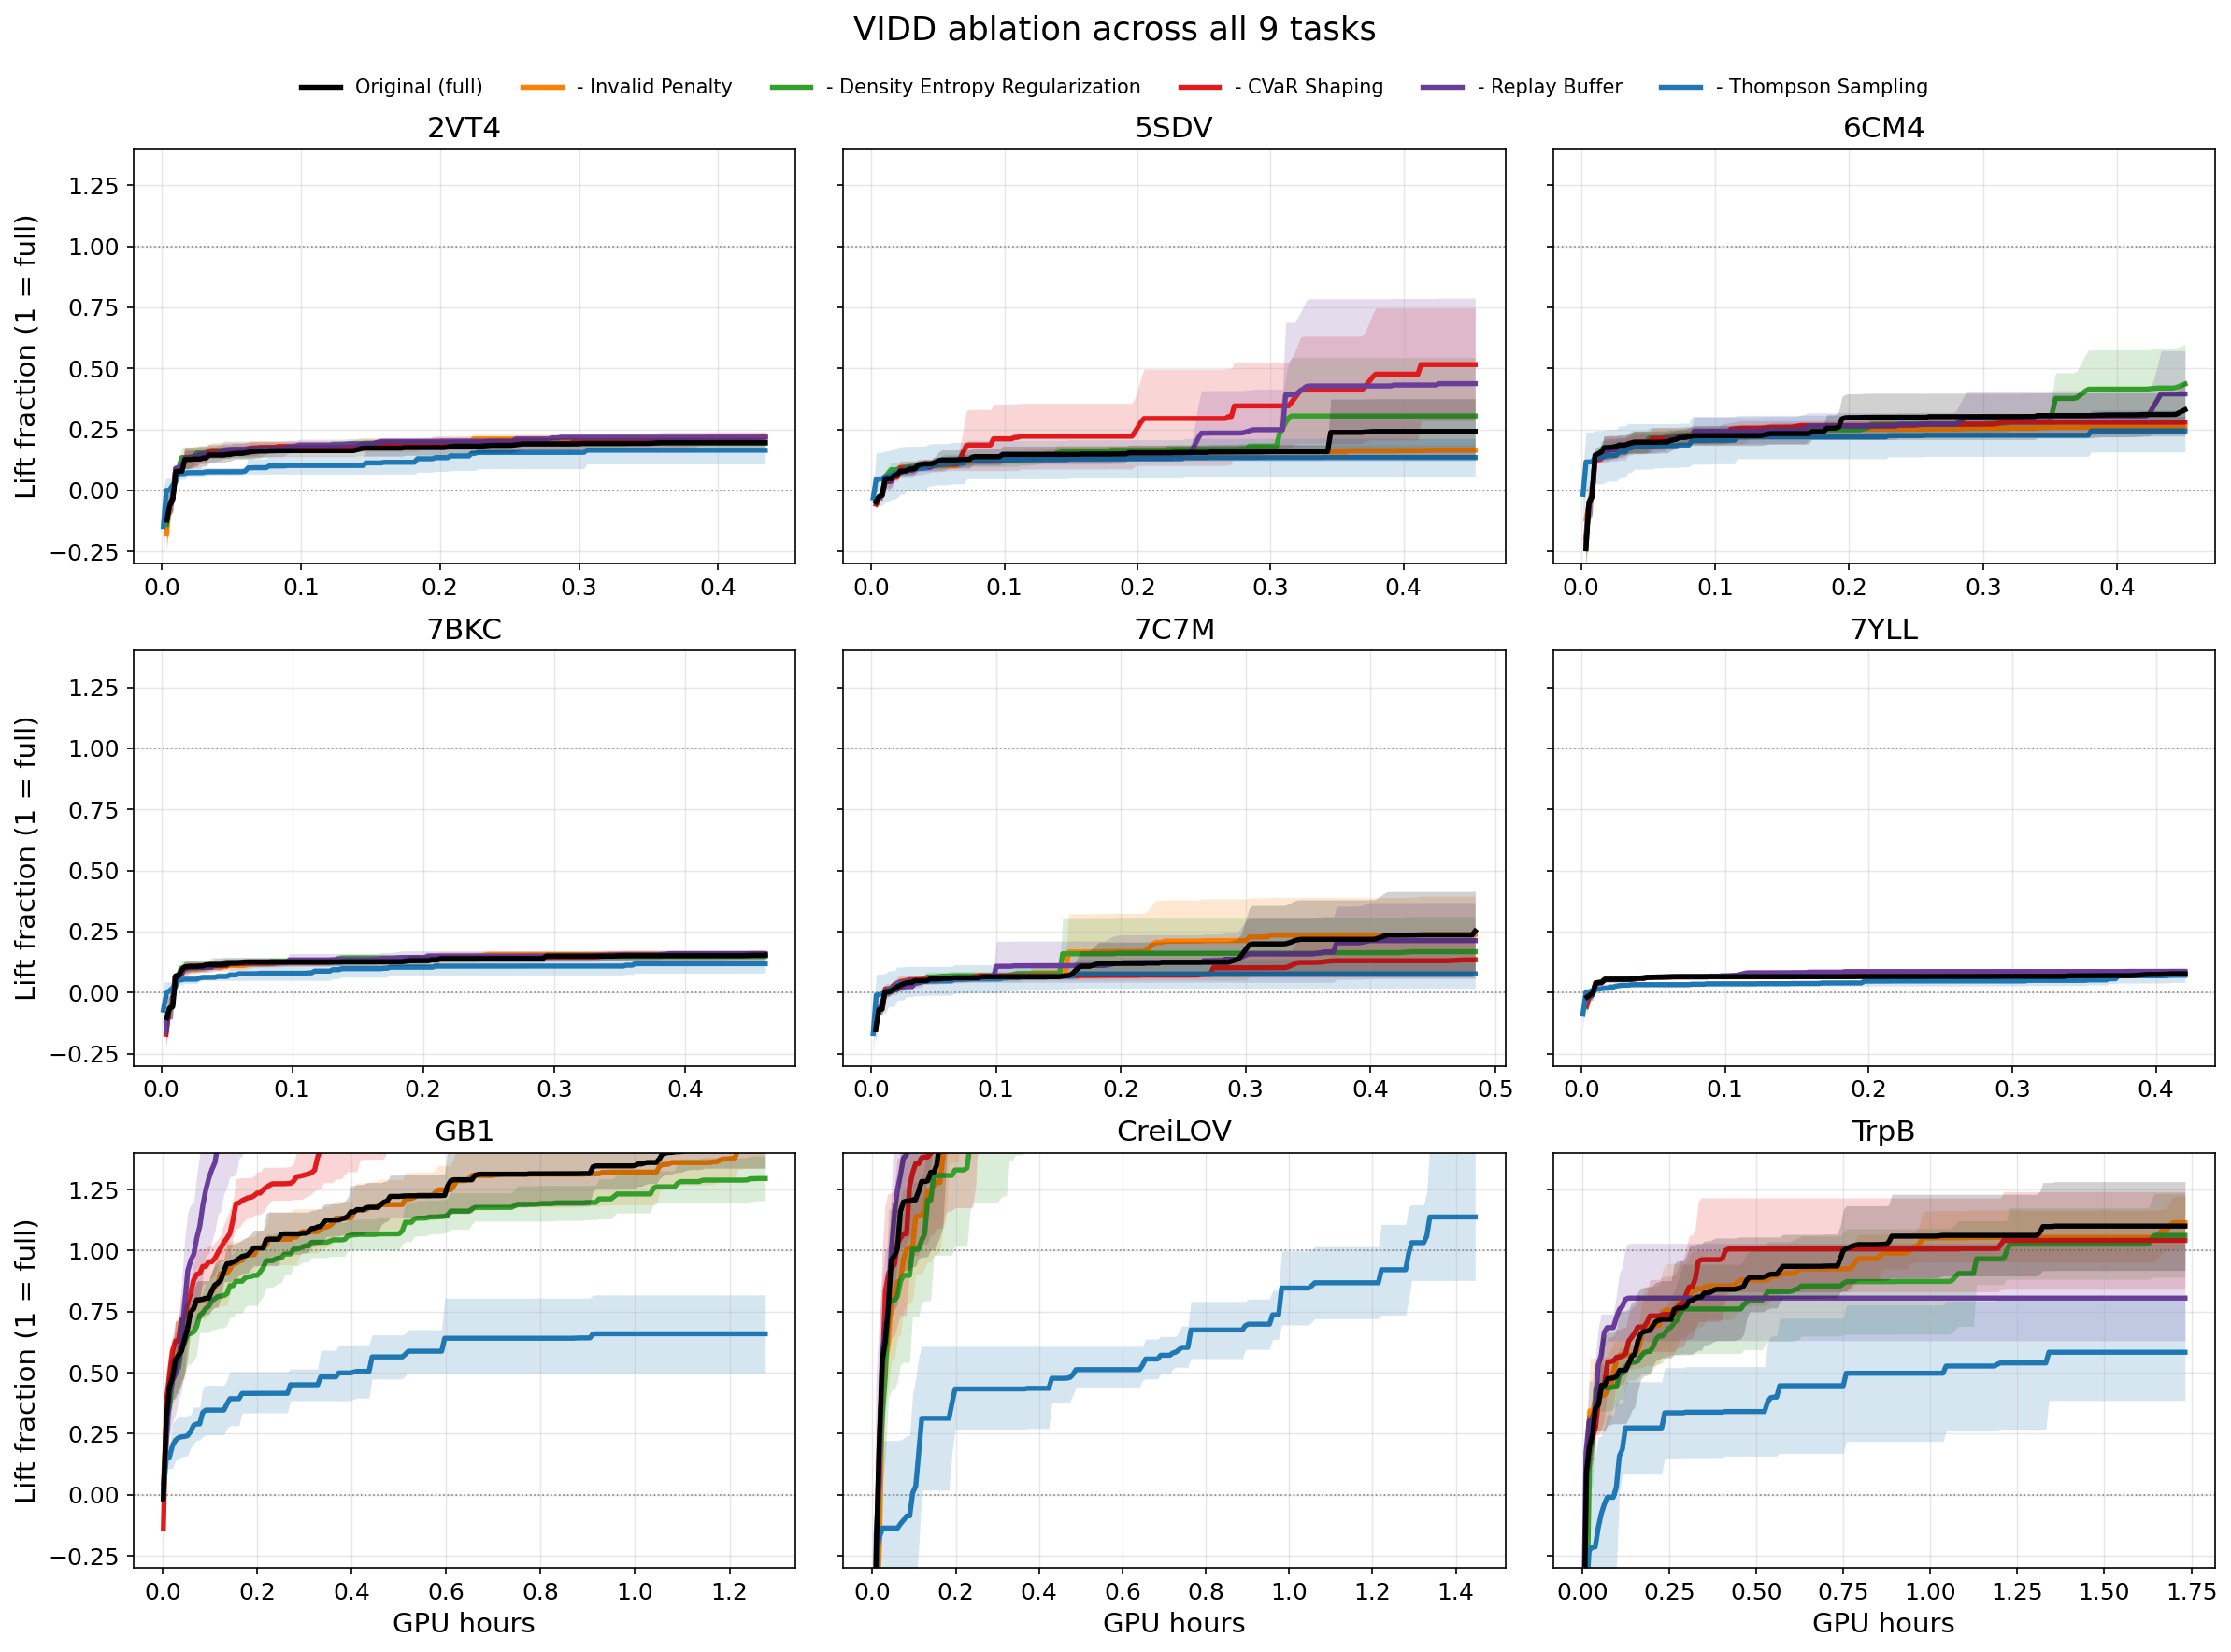
\includegraphics[width=0.95\textwidth]{figures/ablations/vidd_only_grid_norm_gpuhrs.png}
%   \caption{\textbf{VIDD harness ablation, GPU-hours view.} GPU-hours twin of Fig.~\ref{fig:ablation_vidd}. The distillation step adds a fixed per-round cost, so GPU-hour caps are tighter than the corresponding DDPP-LB caps on the same target; knob ordering is unchanged.}
%   \label{fig:ablation_vidd_gpuhrs}
% \end{figure}

% \begin{figure}[H]
%   \centering
%   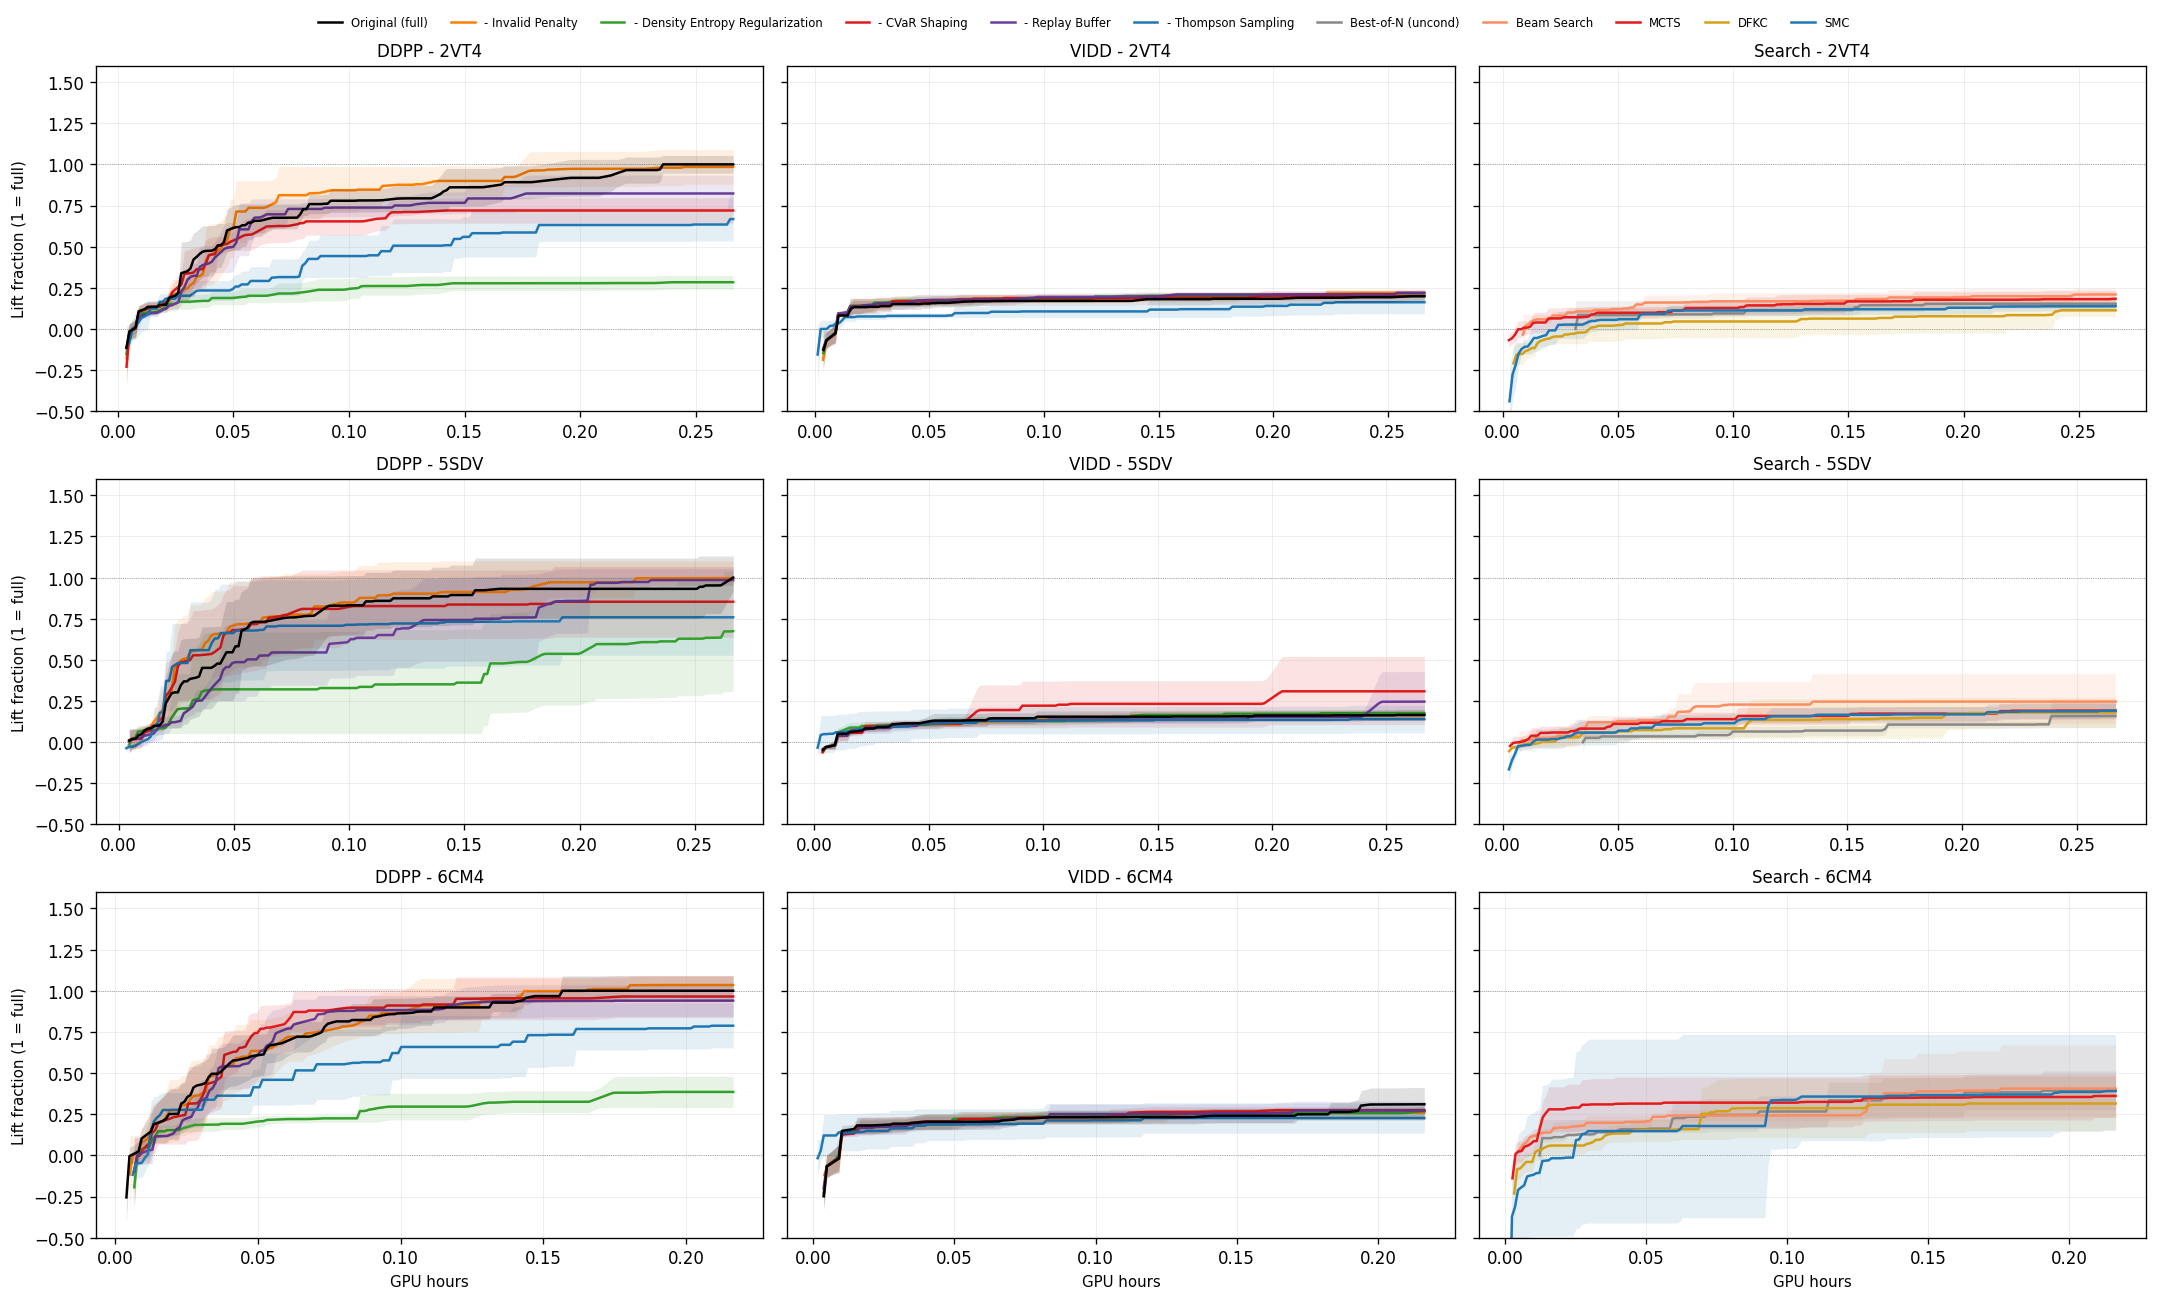
\includegraphics[width=0.95\textwidth]{figures/ablations/mol_ablations_grid_set1_norm_gpuhrs.png}
%   \caption{\textbf{Per-task ablation (mol set 1), GPU-hours view.} GPU-hour twin of Fig.~\ref{fig:per_task_mol_set1}.}
%   \label{fig:per_task_mol_set1_gpuhrs}
% \end{figure}

% \begin{figure}[H]
%   \centering
%   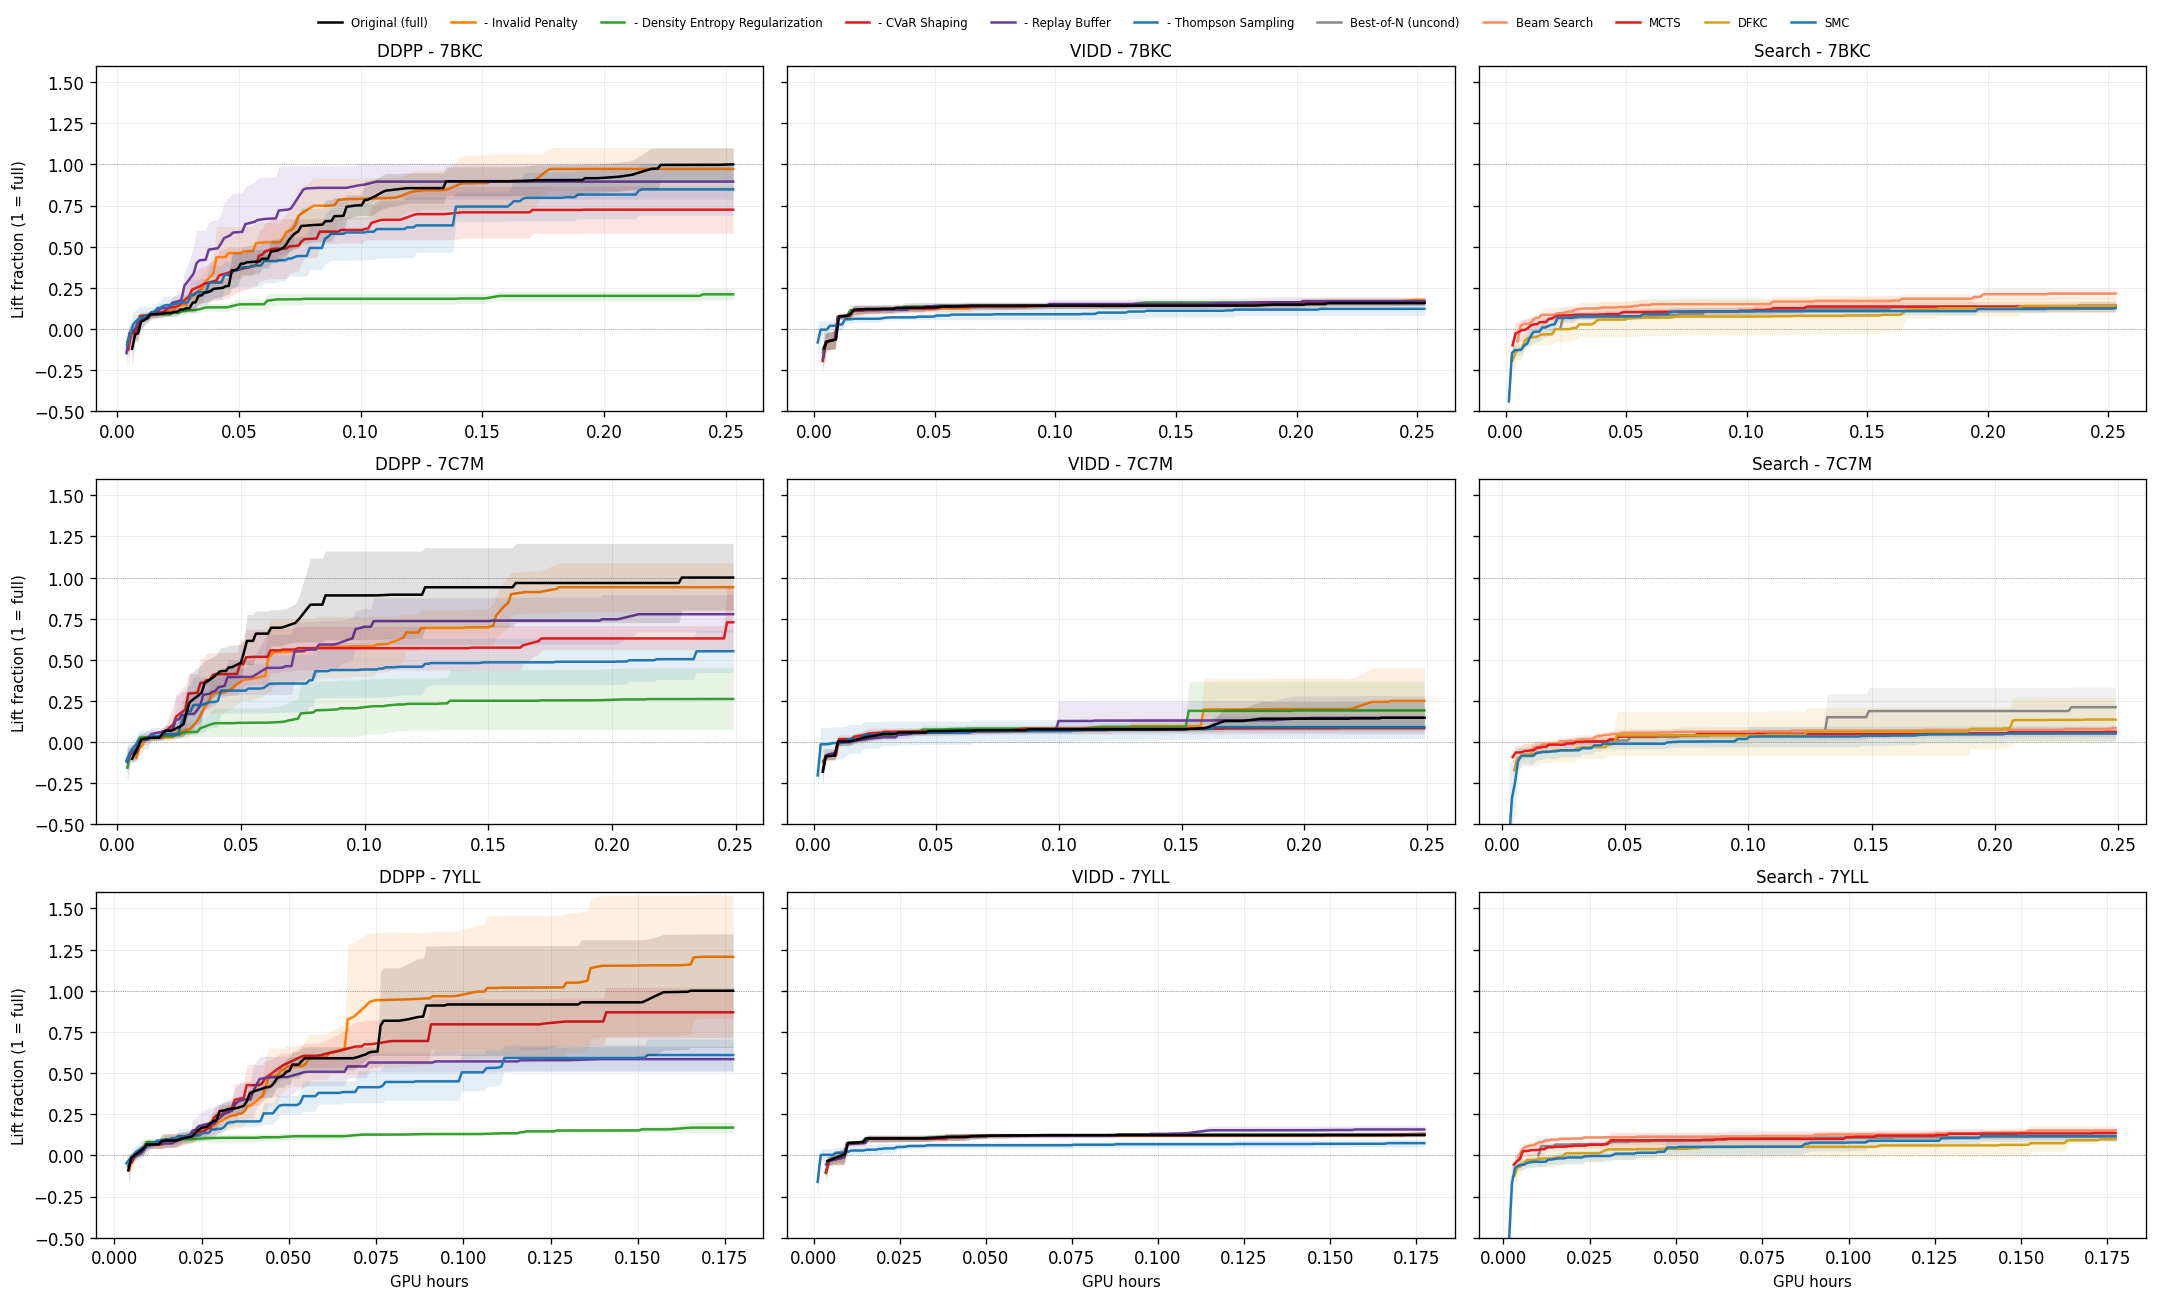
\includegraphics[width=0.95\textwidth]{figures/ablations/mol_ablations_grid_set2_norm_gpuhrs.png}
%   \caption{\textbf{Per-task ablation (mol set 2), GPU-hours view.} GPU-hour twin of Fig.~\ref{fig:per_task_mol_set2}.}
%   \label{fig:per_task_mol_set2_gpuhrs}
% \end{figure}

% \begin{figure}[H]
%   \centering
%   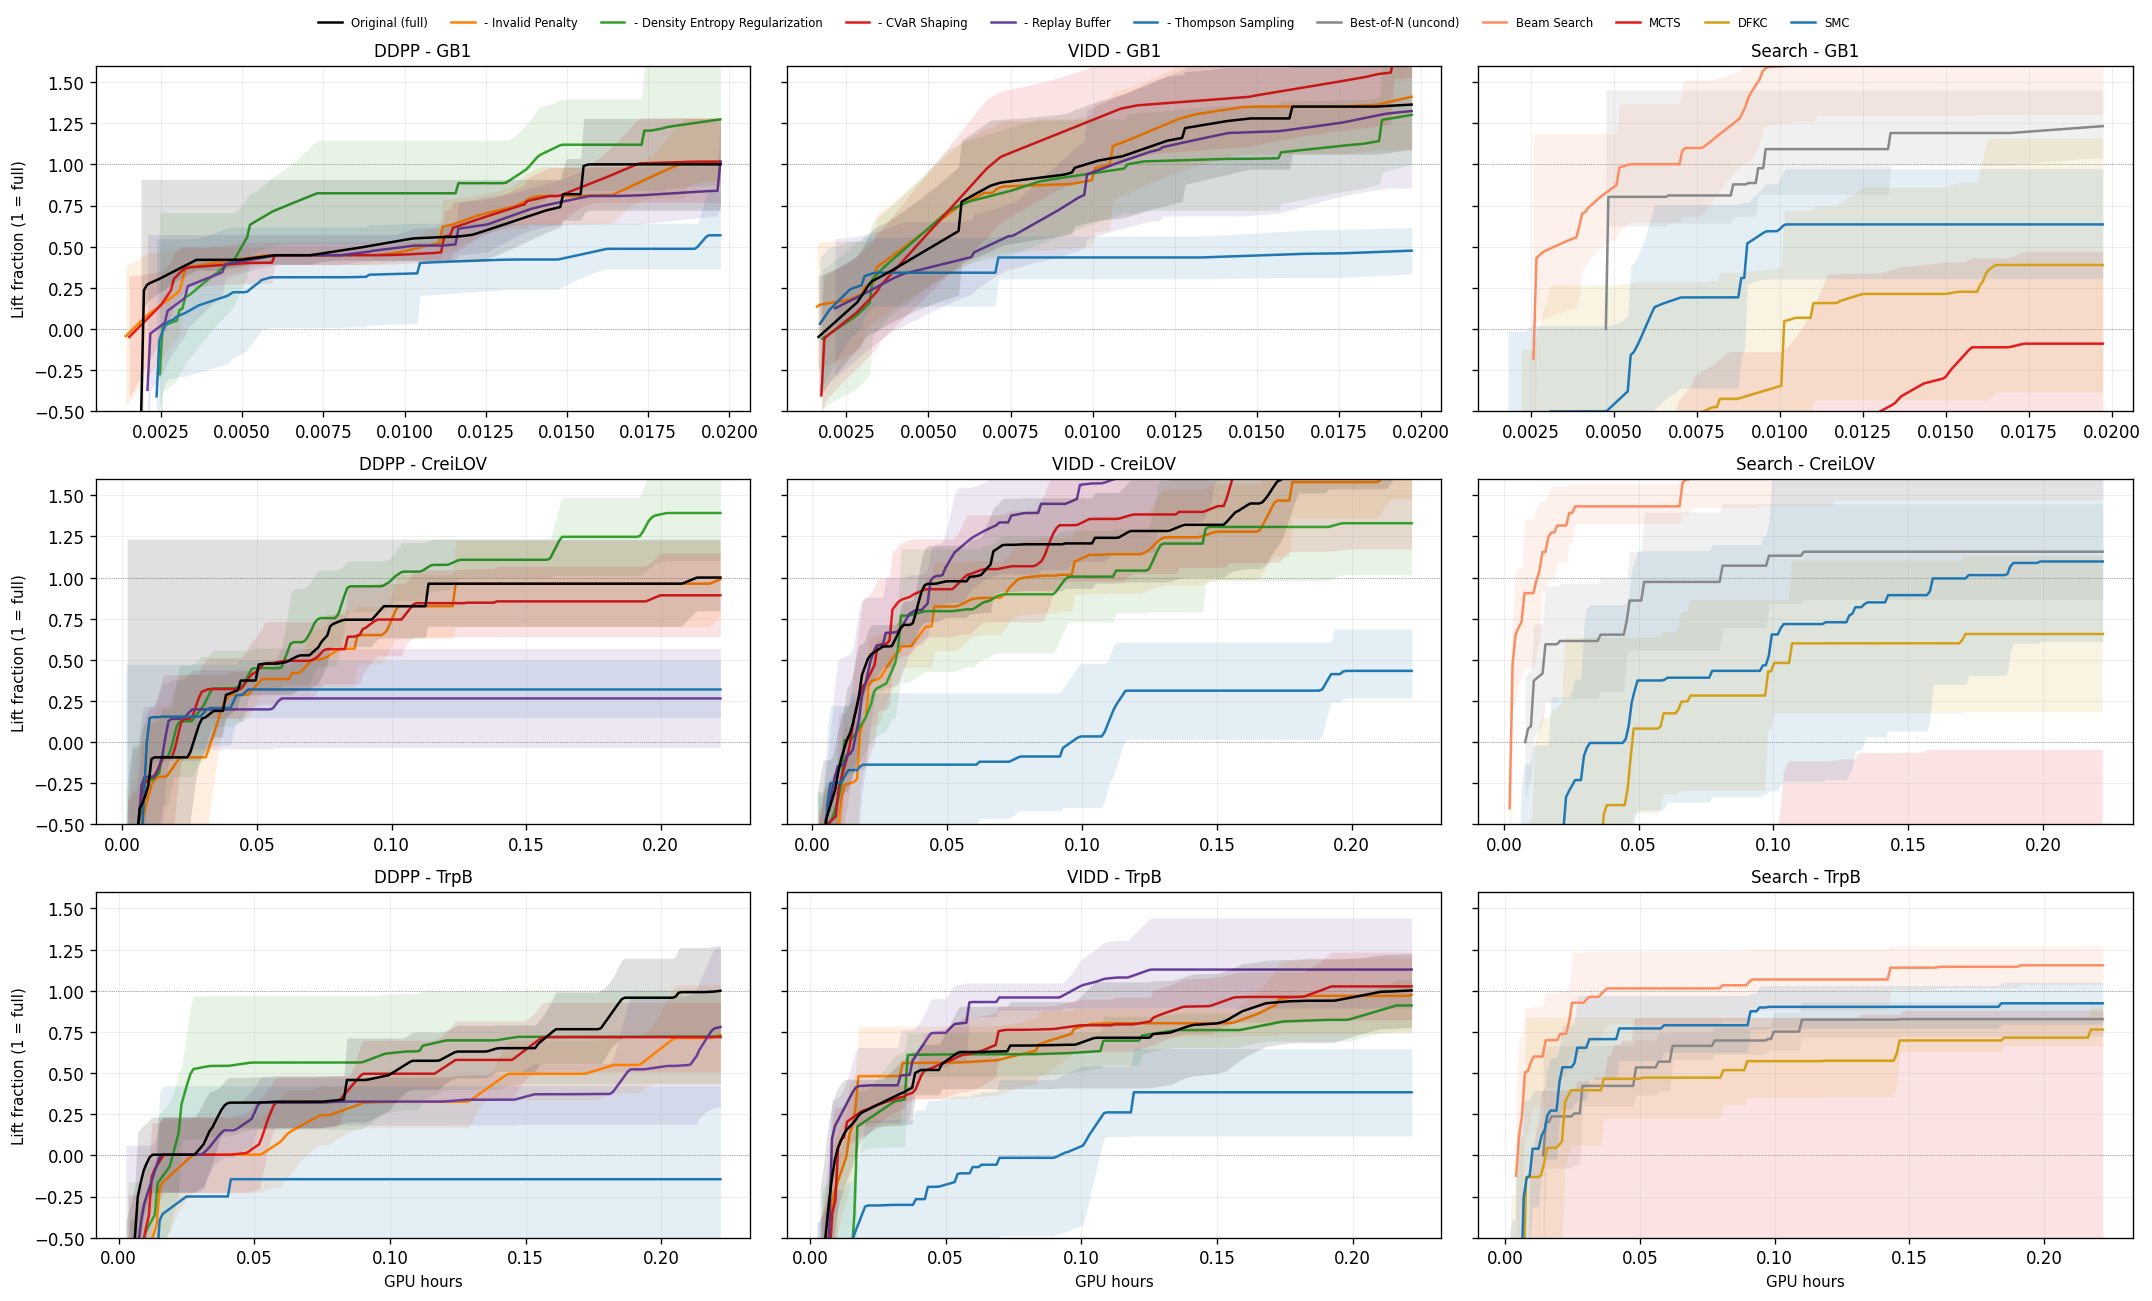
\includegraphics[width=0.95\textwidth]{figures/ablations/protein_ablations_grid_norm_gpuhrs.png}
%   \caption{\textbf{Per-task ablation (proteins), GPU-hours view.} GPU-hour twin of Fig.~\ref{fig:per_task_protein}.}
%   \label{fig:per_task_protein_gpuhrs}
% \end{figure}

\clearpage

\section{Alternative Oracle and Qualitative Examples}\label{app:external-validation}

These experiments test whether the conclusions persist beyond the primary FlashAffinity evaluation and show representative valid outputs.

% Previous heading: \section{Boltz-2 oracle results}\label{app:boltz}
\subsection{Boltz-2 Oracle Results}\label{app:boltz}

The body claims that the design-space conclusions transfer from FlashAffinity (FA) to a structure-prediction-based oracle that is two orders of magnitude more expensive (Sec.~\ref{sec:exp-setup}). This appendix replicates each comparison from Appendices~\ref{app:search} and~\ref{app:knobs} under Boltz-2, with a $10$-hour wall budget per seed. The Boltz-2 panels use the same five seeds (\{0, 1, 2, 3, 42\}) and the same per-knob configurations as their FA counterparts; ablation cells that did not get re-run on Boltz-2 (annealed-CVaR variants, search-side Tweedie variants) are omitted. We show top-1 best-so-far against cumulative oracle calls (left) and GPU hours (right) only --- the top-10 / top-10\% rows from Appendix~\ref{app:knobs} are not separately rendered for Boltz-2. Across every panel below the relative ordering of methods is preserved, supporting the claim that the recipe is robust to oracle expense.

\begin{figure}[H]
  \centering
  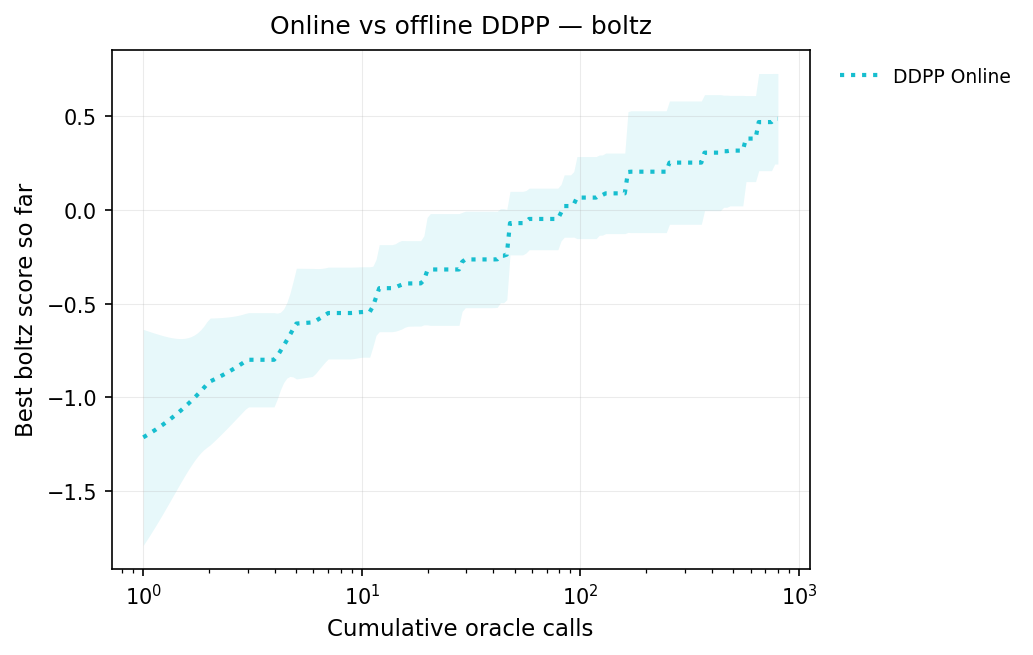
\includegraphics[width=0.49\textwidth]{figures/boltz_online_offline_a.png}\hfill
  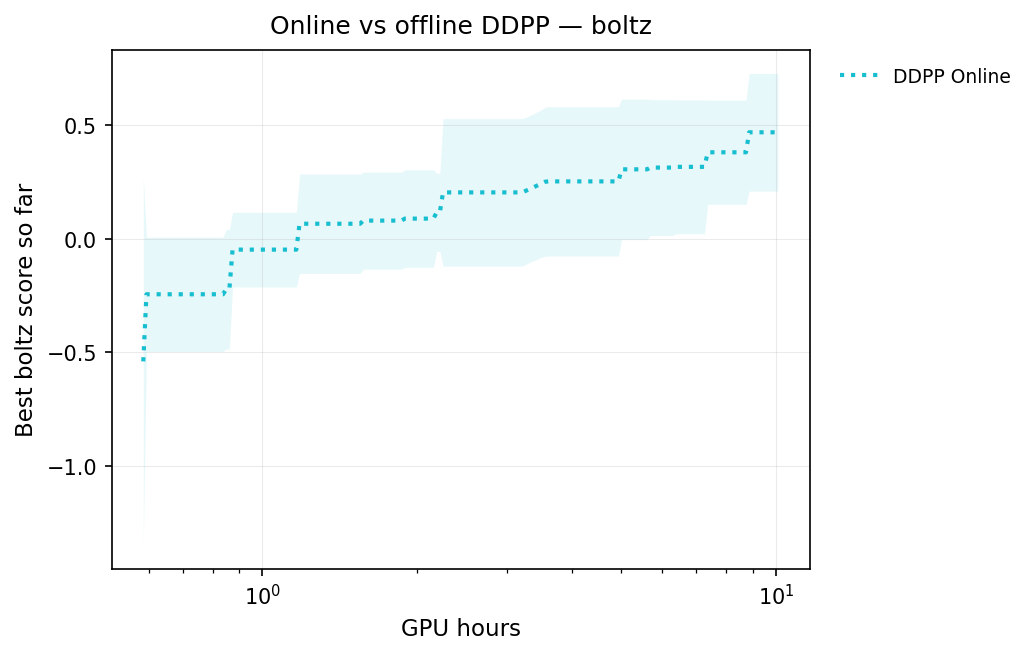
\includegraphics[width=0.49\textwidth]{figures/boltz_online_offline_b.png}
  \caption{\textbf{Online vs.\ offline DDPP-LB --- Boltz-2.} Companion to Fig.~\ref{fig:online_vs_offline}. Same conclusion: online dominates offline at matched compute on top-1 best-so-far Boltz-2 score.}
  \label{fig:boltz_online_offline}
\end{figure}

\begin{figure}[H]
  \centering
  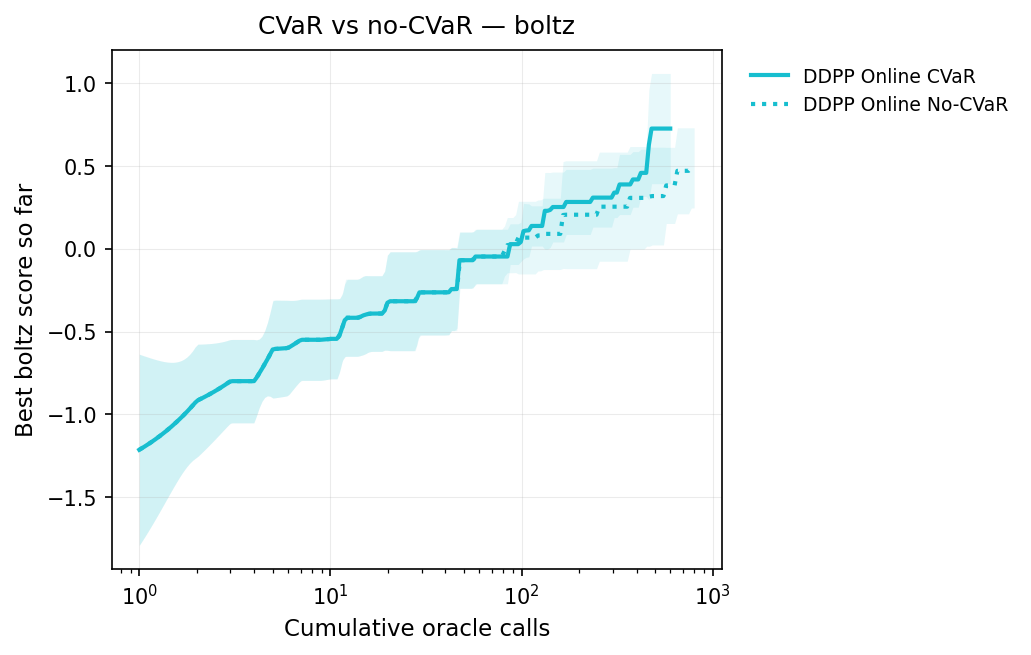
\includegraphics[width=0.49\textwidth]{figures/boltz_cvar_a.png}\hfill
  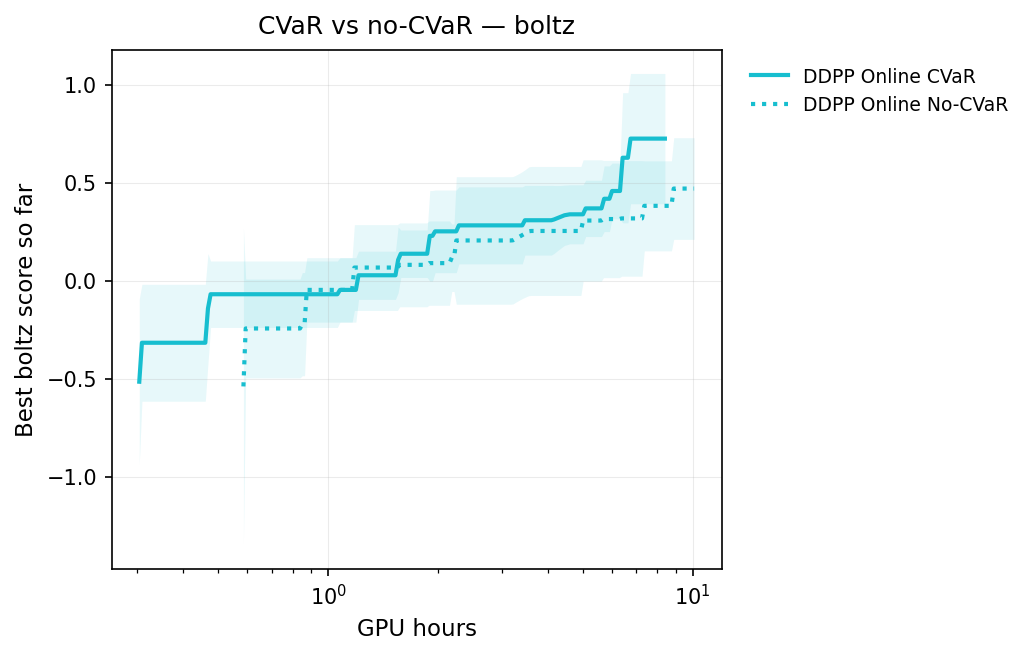
\includegraphics[width=0.49\textwidth]{figures/boltz_cvar_b.png}
  \caption{\textbf{CVaR ablation --- Boltz-2.} Companion to Fig.~\ref{fig:cvar_ablation}, online cells only (offline DDPP was not re-run on Boltz-2). CVaR-on solid, CVaR-off dotted. CVaR continues to lift top-1 by a comparable margin under Boltz-2 as under FA.}
  \label{fig:boltz_cvar}
\end{figure}

\begin{figure}[H]
  \centering
  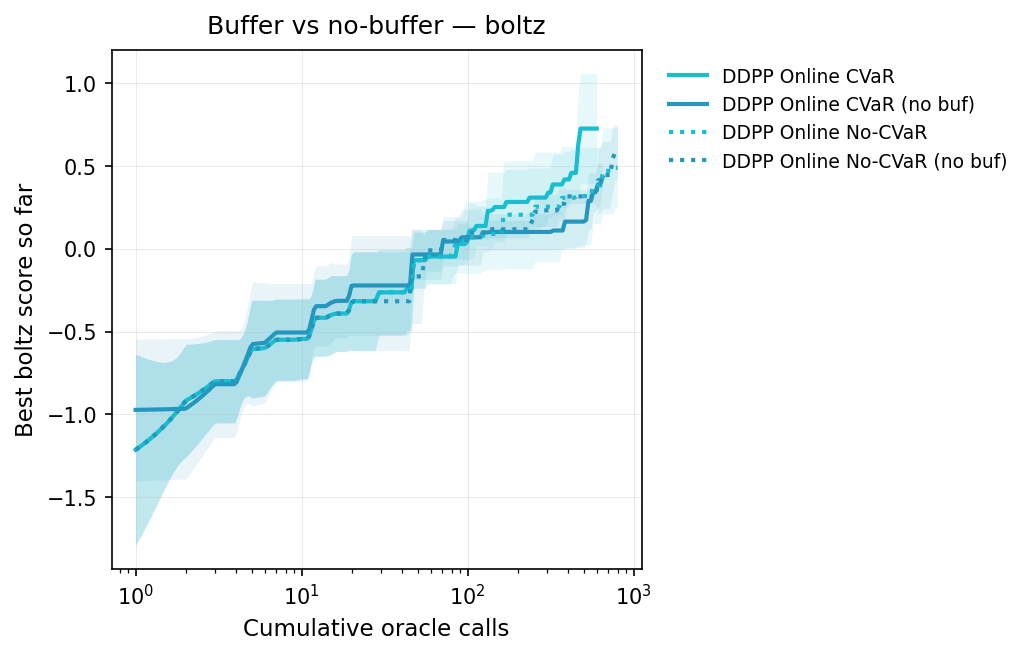
\includegraphics[width=0.49\textwidth]{figures/boltz_buffer_a.png}\hfill
  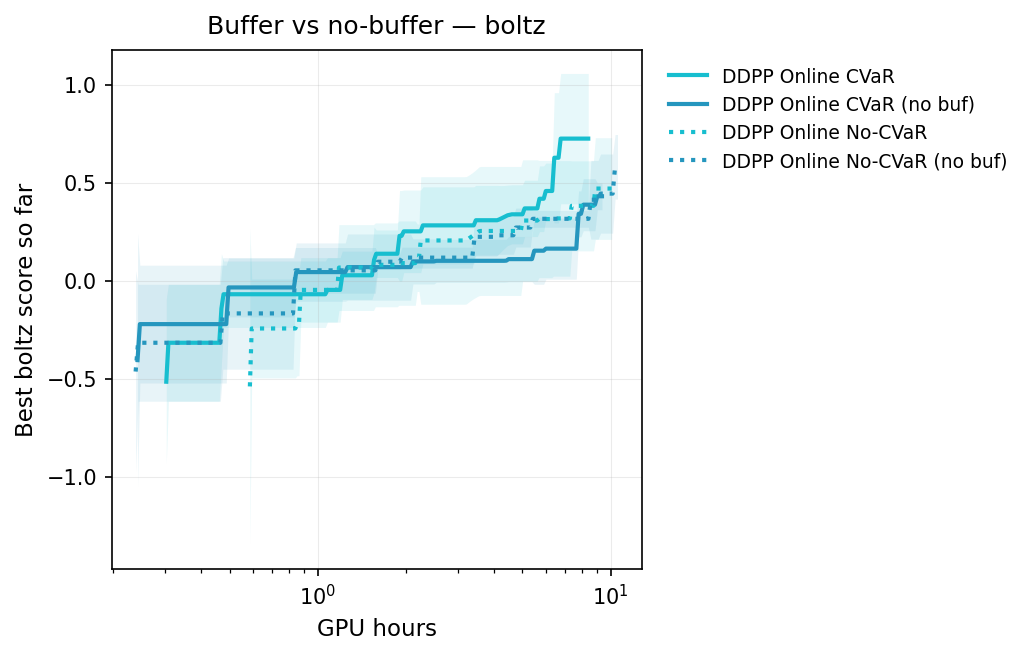
\includegraphics[width=0.49\textwidth]{figures/boltz_buffer_b.png}
  \caption{\textbf{Replay-buffer ablation --- Boltz-2.} Companion to Fig.~\ref{fig:buffer_ablation}. Same four cells as the FA version (buffer~$\times$~CVaR). The buffer-on / CVaR-on cell continues to lead.}
  \label{fig:boltz_buffer}
\end{figure}

\begin{figure}[H]
  \centering
  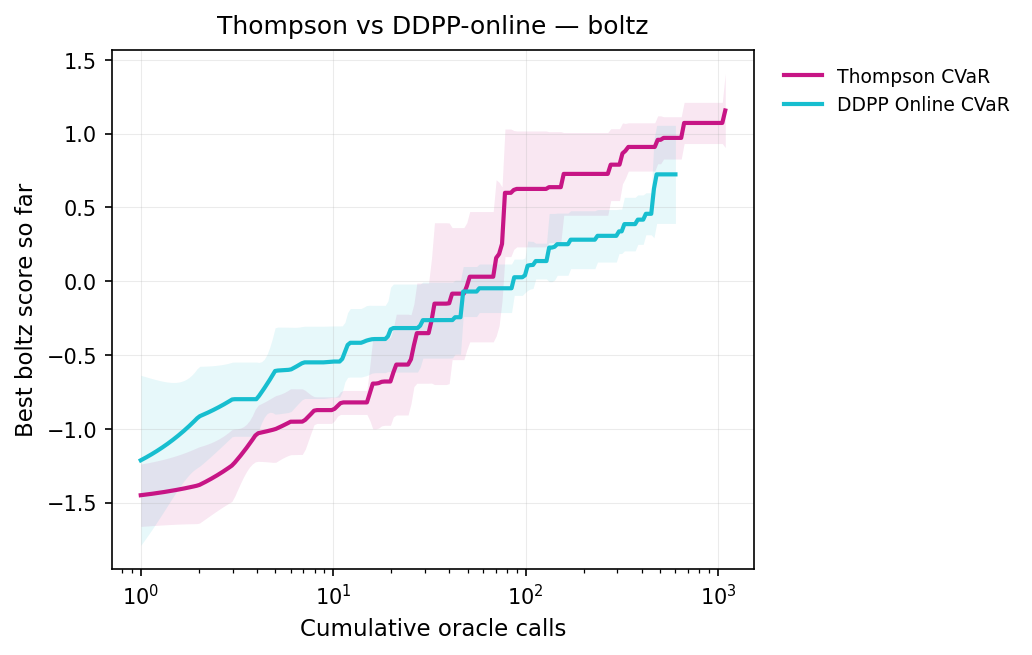
\includegraphics[width=0.49\textwidth]{figures/boltz_thompson_a.png}\hfill
  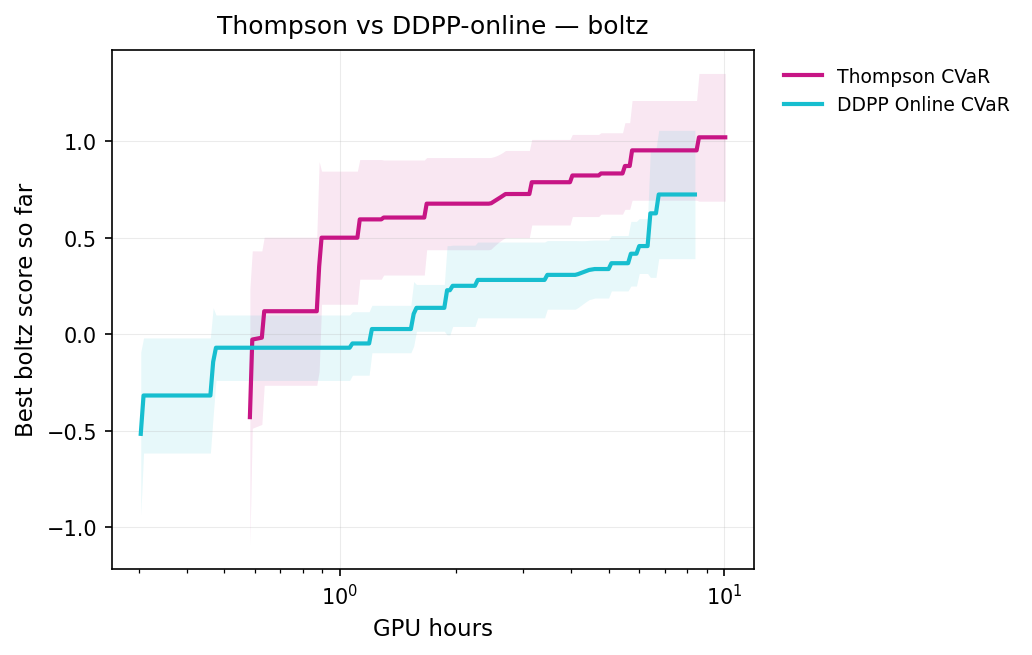
\includegraphics[width=0.49\textwidth]{figures/boltz_thompson_b.png}
  \caption{\textbf{Thompson-sampling ablation --- Boltz-2.} Companion to Fig.~\ref{fig:thompson_ablation}. Thompson on top of online DDPP-LB$+$CVaR vs.\ deterministic top-$K$ selection. Thompson retains its lead on top-1 under the slower oracle.}
  \label{fig:boltz_thompson}
\end{figure}

\begin{figure}[H]
  \centering
  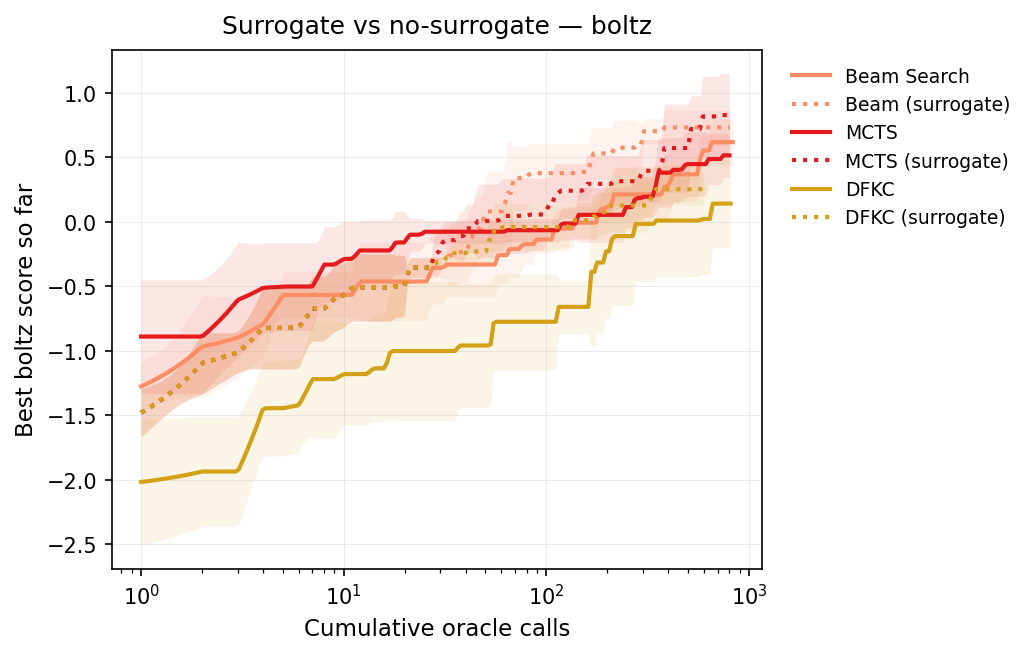
\includegraphics[width=0.49\textwidth]{figures/boltz_surrogate_a.png}\hfill
  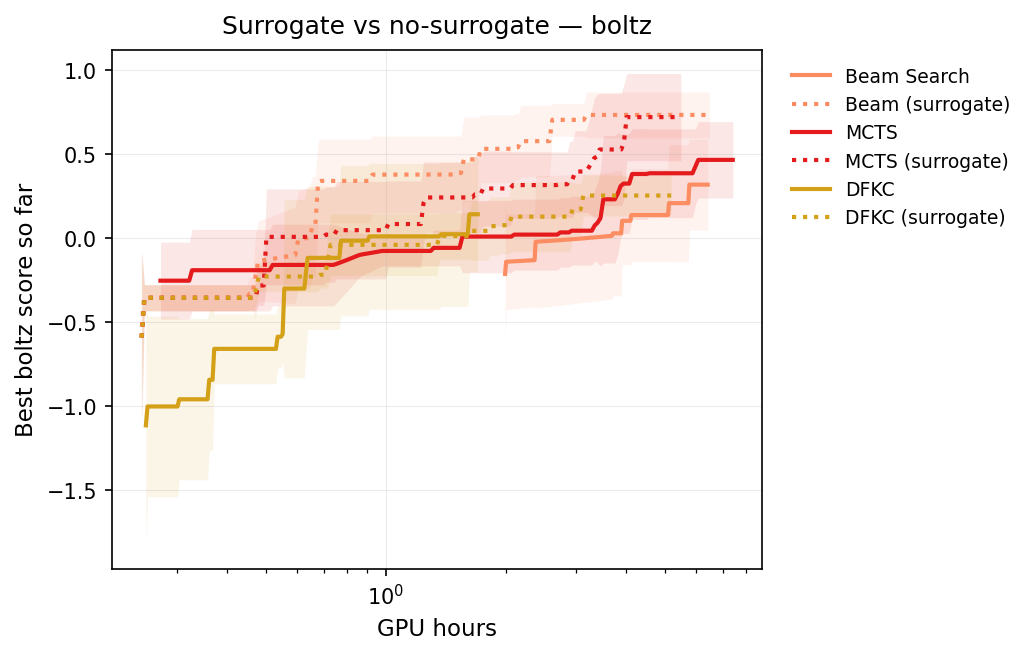
\includegraphics[width=0.49\textwidth]{figures/boltz_surrogate_b.png}
  \caption{\textbf{Surrogate screening on inference-time search --- Boltz-2.} Companion to Fig.~\ref{fig:surrogate_search}. Beam, MCTS, and DFKC each compared against their surrogate-pre-filter variant. Surrogate screening continues to dominate plain search across all three families under Boltz-2.}
  \label{fig:boltz_surrogate}
\end{figure}

\begin{figure}[H]
  \centering
  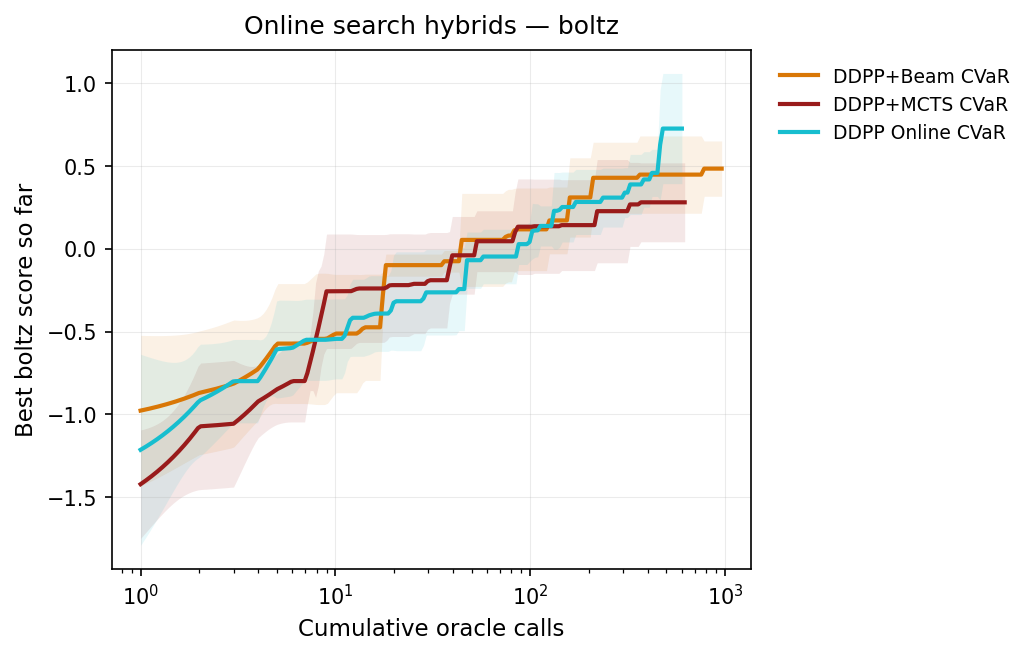
\includegraphics[width=0.49\textwidth]{figures/boltz_oracle_rescale_1x_a.png}\hfill
  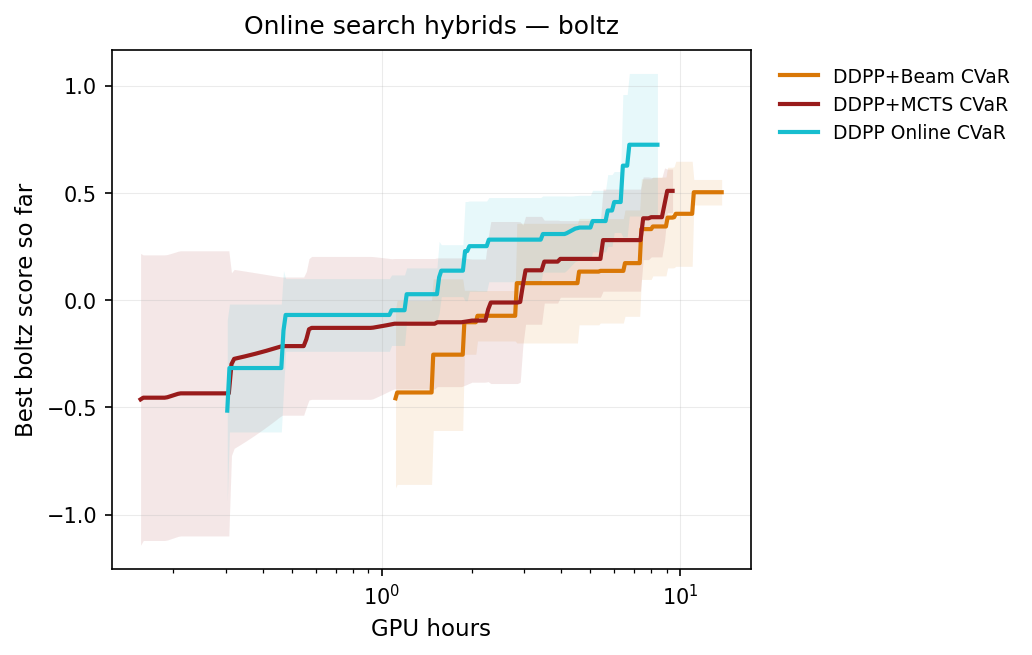
\includegraphics[width=0.49\textwidth]{figures/boltz_oracle_rescale_1x_b.png}
  \caption{\textbf{Online search hybrids at standard Boltz-2 oracle cost.} Plain online DDPP-LB$+$CVaR vs.\ DDPP$+$beam$+$CVaR vs.\ DDPP$+$MCTS$+$CVaR. Plain online matches or exceeds both search-augmented variants on top-1 Boltz-2, mirroring the FA conclusion in Sec.~\ref{sec:results}.}
  \label{fig:boltz_oracle_1x}
\end{figure}

\begin{figure}[H]
  \centering
  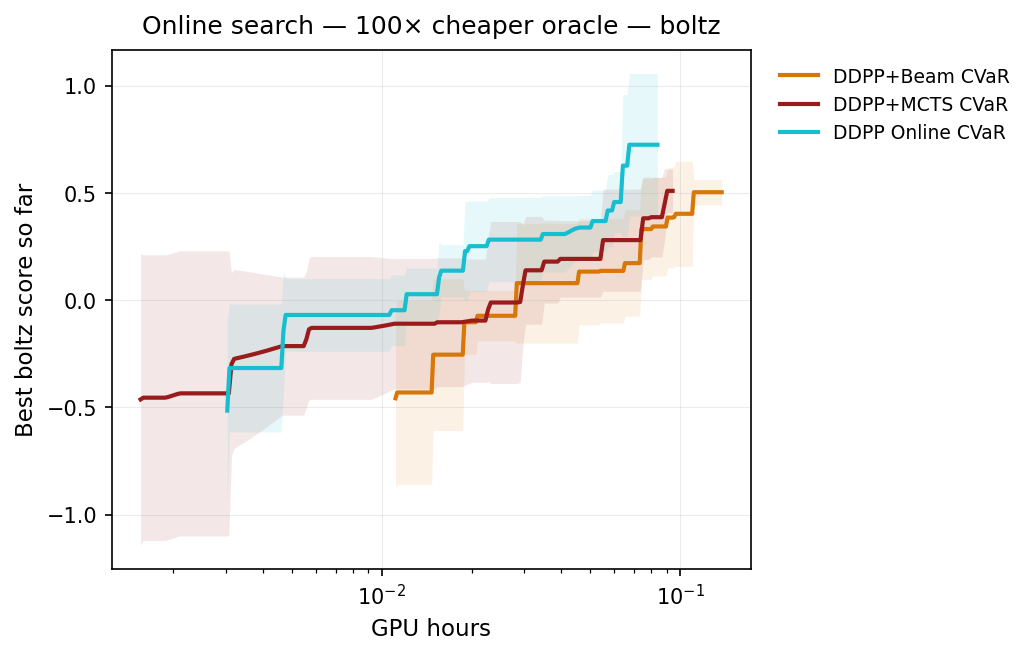
\includegraphics[width=0.49\textwidth]{figures/boltz_oracle_rescale_cheaper_b.png}\hfill
  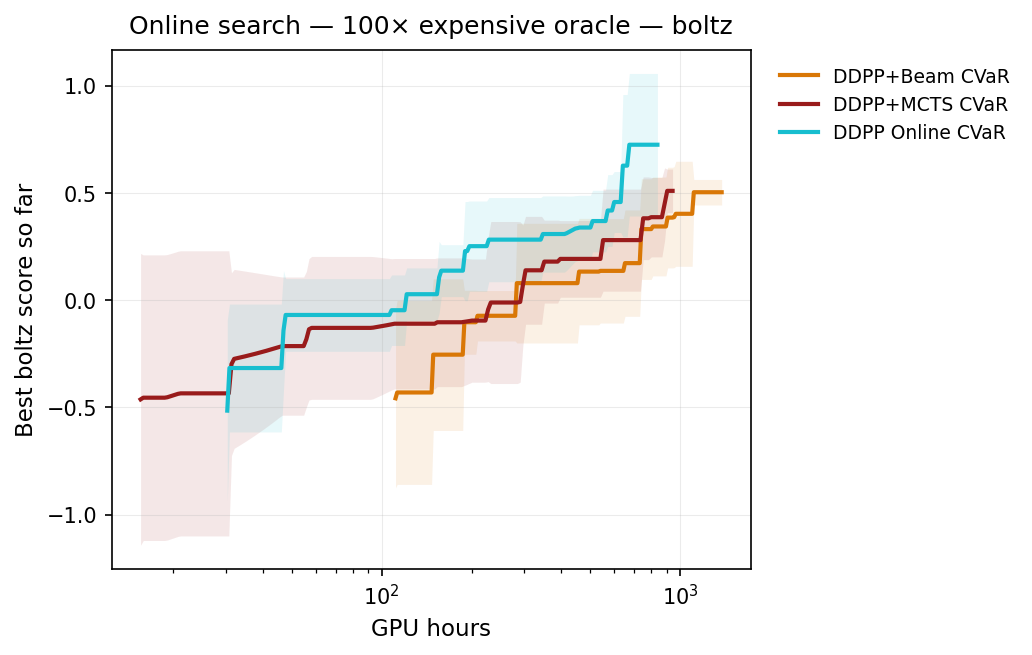
\includegraphics[width=0.49\textwidth]{figures/boltz_oracle_rescale_expensive_b.png}
  \caption{\textbf{Retroactive Boltz-2 oracle-cost rescaling.} Companion to Fig.~\ref{fig:oracle_rescale}, restricted to the GPU-hours axis. Per-call Boltz-2 cost rescaled by $1/100$ (left) and $100$ (right). The rescaling shifts the GPU-hours axis by four orders of magnitude in either direction without altering the relative ordering: plain online DDPP-LB$+$CVaR continues to match or exceed the search-augmented variants under both regimes, supporting the claim that the marginal value of inference-time search on top of online finetuning is robust to oracle expense even when the oracle is itself the expensive variant.}
  \label{fig:boltz_oracle_rescale}
\end{figure}

% Previous heading: \section{Valid molecule samples across targets and methods}
\subsection{Valid Molecule Samples Across Targets and Methods}\label{app:valid-samples}

For the FA-oracle small-molecule targets, we render
representative oracle-evaluated SMILES generated by the \textbf{DDPP-LB}
and \textbf{VIDD} full methods. Per (method, target) we display
three \emph{high-score} picks (top decile of all oracle calls) and three
\emph{low-score} picks (bottom decile). 

\begin{figure}[H]
\centering
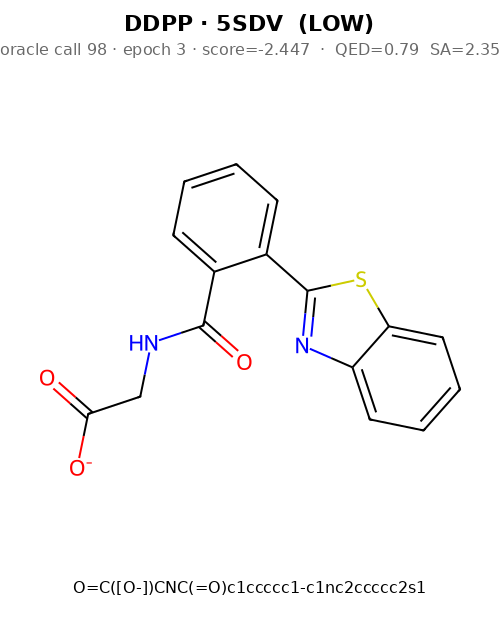
\includegraphics[width=0.31\textwidth]{image2.png}\hfill
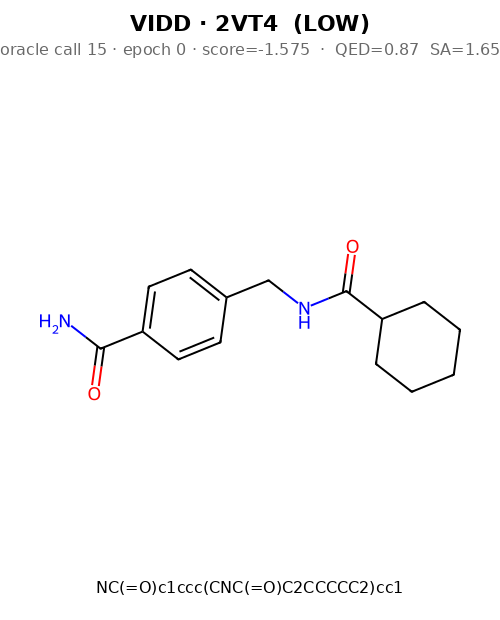
\includegraphics[width=0.31\textwidth]{image4.png}\hfill
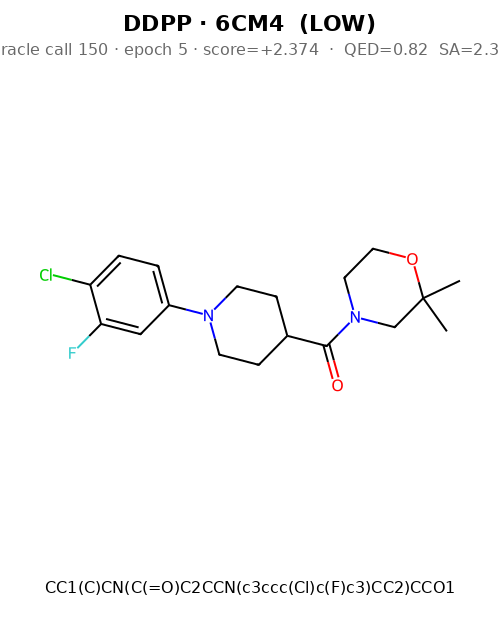
\includegraphics[width=0.31\textwidth]{image3.png}

\vspace{0.6em}

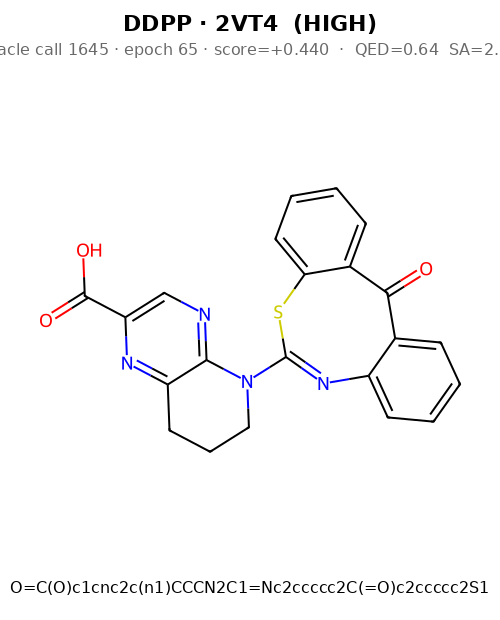
\includegraphics[width=0.31\textwidth]{image5.png}\hfill
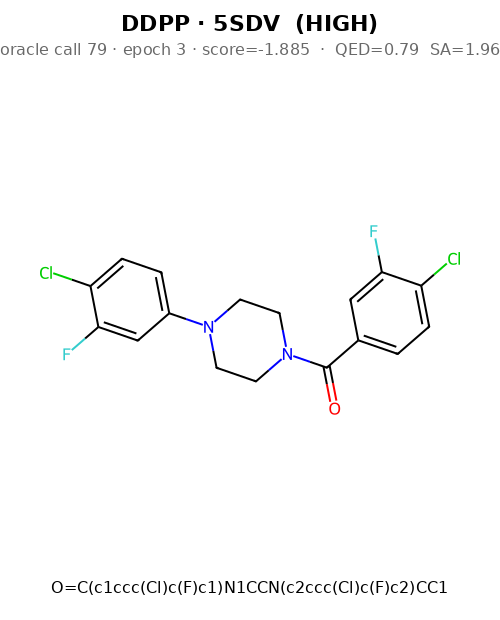
\includegraphics[width=0.31\textwidth]{image6.png}\hfill
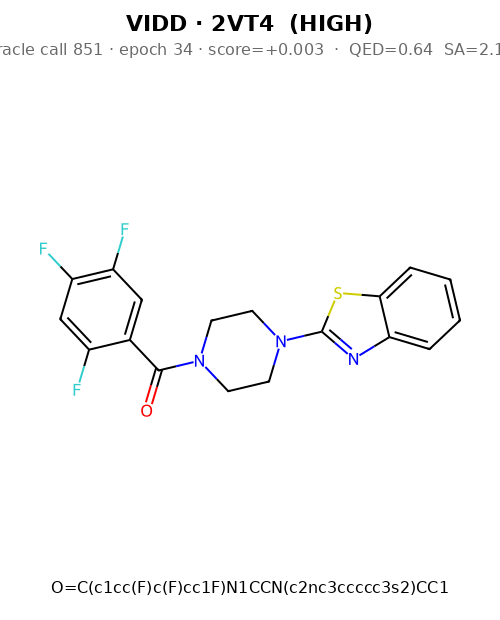
\includegraphics[width=0.31\textwidth]{image7.png}
\end{figure}
%%%%%%%%%%%%%%%%%%%%%%%%%%%%%%%%%%%%%%%%%%%%%%%%%%%%%%%%%%%%

\clearpage

\section{Declaration of LLM Usage}
LLMs were used to write code, interpret results, assist with writing, and assist with figure making.

\clearpage
\section*{NeurIPS Paper Checklist}

% %%% BEGIN INSTRUCTIONS %%%
% The checklist is designed to encourage best practices for responsible machine learning research, addressing issues of reproducibility, transparency, research ethics, and societal impact. Do not remove the checklist: {\bf The papers not including the checklist will be desk rejected.} The checklist should follow the references and follow the (optional) supplemental material.  The checklist does NOT count towards the page
% limit. 
% 
% Please read the checklist guidelines carefully for information on how to answer these questions. For each question in the checklist:
% \begin{itemize}
%     \item You should answer \answerYes{}, \answerNo{}, or \answerNA{}.
%     \item \answerNA{} means either that the question is Not Applicable for that particular paper or the relevant information is Not Available.
%     \item Please provide a short (1--2 sentence) justification right after your answer (even for \answerNA). 
%    % \item {\bf The papers not including the checklist will be desk rejected.}
% \end{itemize}
% 
% {\bf The checklist answers are an integral part of your paper submission.} They are visible to the reviewers, area chairs, senior area chairs, and ethics reviewers. You will also be asked to include it (after eventual revisions) with the final version of your paper, and its final version will be published with the paper.
% 
% The reviewers of your paper will be asked to use the checklist as one of the factors in their evaluation. While \answerYes{} is generally preferable to \answerNo{}, it is perfectly acceptable to answer \answerNo{} provided a proper justification is given (e.g., error bars are not reported because it would be too computationally expensive'' or ``we were unable to find the license for the dataset we used''). In general, answering \answerNo{} or \answerNA{} is not grounds for rejection. While the questions are phrased in a binary way, we acknowledge that the true answer is often more nuanced, so please just use your best judgment and write a justification to elaborate. All supporting evidence can appear either in the main paper or the supplemental material, provided in appendix. If you answer \answerYes{} to a question, in the justification please point to the section(s) where related material for the question can be found.
% 
% IMPORTANT, please:
% \begin{itemize}
%     \item {\bf Delete this instruction block, but keep the section heading ``NeurIPS Paper Checklist"},
%     \item  {\bf Keep the checklist subsection headings, questions/answers and guidelines below.}
%     \item {\bf Do not modify the questions and only use the provided macros for your answers}.
% \end{itemize} 
%  
% 
% %%% END INSTRUCTIONS %%%


\begin{enumerate}

\item {\bf Claims}
    \item[] Question: Do the main claims made in the abstract and introduction accurately reflect the paper's contributions and scope?
    \item[] Answer: \answerYes{} % Replace by \answerYes{}, \answerNo{}, or \answerNA{}.
    \item[] Justification: The claims reflect the empirical results that we have collected.
    \item[] Guidelines:
    \begin{itemize}
        \item The answer \answerNA{} means that the abstract and introduction do not include the claims made in the paper.
        \item The abstract and/or introduction should clearly state the claims made, including the contributions made in the paper and important assumptions and limitations. A \answerNo{} or \answerNA{} answer to this question will not be perceived well by the reviewers. 
        \item The claims made should match theoretical and experimental results, and reflect how much the results can be expected to generalize to other settings. 
        \item It is fine to include aspirational goals as motivation as long as it is clear that these goals are not attained by the paper. 
    \end{itemize}

\item {\bf Limitations}
    \item[] Question: Does the paper discuss the limitations of the work performed by the authors?
    \item[] Answer: \answerYes{} % Replace by \answerYes{}, \answerNo{}, or \answerNA{}.
    \item[] Justification: Limitations are provided in the discussion section.
    \item[] Guidelines:
    \begin{itemize}
        \item The answer \answerNA{} means that the paper has no limitation while the answer \answerNo{} means that the paper has limitations, but those are not discussed in the paper. 
        \item The authors are encouraged to create a separate ``Limitations'' section in their paper.
        \item The paper should point out any strong assumptions and how robust the results are to violations of these assumptions (e.g., independence assumptions, noiseless settings, model well-specification, asymptotic approximations only holding locally). The authors should reflect on how these assumptions might be violated in practice and what the implications would be.
        \item The authors should reflect on the scope of the claims made, e.g., if the approach was only tested on a few datasets or with a few runs. In general, empirical results often depend on implicit assumptions, which should be articulated.
        \item The authors should reflect on the factors that influence the performance of the approach. For example, a facial recognition algorithm may perform poorly when image resolution is low or images are taken in low lighting. Or a speech-to-text system might not be used reliably to provide closed captions for online lectures because it fails to handle technical jargon.
        \item The authors should discuss the computational efficiency of the proposed algorithms and how they scale with dataset size.
        \item If applicable, the authors should discuss possible limitations of their approach to address problems of privacy and fairness.
        \item While the authors might fear that complete honesty about limitations might be used by reviewers as grounds for rejection, a worse outcome might be that reviewers discover limitations that aren't acknowledged in the paper. The authors should use their best judgment and recognize that individual actions in favor of transparency play an important role in developing norms that preserve the integrity of the community. Reviewers will be specifically instructed to not penalize honesty concerning limitations.
    \end{itemize}

\item {\bf Theory assumptions and proofs}
    \item[] Question: For each theoretical result, does the paper provide the full set of assumptions and a complete (and correct) proof?
    \item[] Answer: \answerNA{} % Replace by \answerYes{}, \answerNo{}, or \answerNA{}.
    \item[] Justification: No new theories are derived in this paper.
    \item[] Guidelines:
    \begin{itemize}
        \item The answer \answerNA{} means that the paper does not include theoretical results. 
        \item All the theorems, formulas, and proofs in the paper should be numbered and cross-referenced.
        \item All assumptions should be clearly stated or referenced in the statement of any theorems.
        \item The proofs can either appear in the main paper or the supplemental material, but if they appear in the supplemental material, the authors are encouraged to provide a short proof sketch to provide intuition. 
        \item Inversely, any informal proof provided in the core of the paper should be complemented by formal proofs provided in appendix or supplemental material.
        \item Theorems and Lemmas that the proof relies upon should be properly referenced. 
    \end{itemize}

    \item {\bf Experimental result reproducibility}
    \item[] Question: Does the paper fully disclose all the information needed to reproduce the main experimental results of the paper to the extent that it affects the main claims and/or conclusions of the paper (regardless of whether the code and data are provided or not)?
    \item[] Answer: \answerYes{} % Replace by \answerYes{}, \answerNo{}, or \answerNA{}.
    \item[] Justification: We provide extensive method details in the main text and the appendix.
    \item[] Guidelines:
    \begin{itemize}
        \item The answer \answerNA{} means that the paper does not include experiments.
        \item If the paper includes experiments, a \answerNo{} answer to this question will not be perceived well by the reviewers: Making the paper reproducible is important, regardless of whether the code and data are provided or not.
        \item If the contribution is a dataset and\slash or model, the authors should describe the steps taken to make their results reproducible or verifiable. 
        \item Depending on the contribution, reproducibility can be accomplished in various ways. For example, if the contribution is a novel architecture, describing the architecture fully might suffice, or if the contribution is a specific model and empirical evaluation, it may be necessary to either make it possible for others to replicate the model with the same dataset, or provide access to the model. In general. releasing code and data is often one good way to accomplish this, but reproducibility can also be provided via detailed instructions for how to replicate the results, access to a hosted model (e.g., in the case of a large language model), releasing of a model checkpoint, or other means that are appropriate to the research performed.
        \item While NeurIPS does not require releasing code, the conference does require all submissions to provide some reasonable avenue for reproducibility, which may depend on the nature of the contribution. For example
        \begin{enumerate}
            \item If the contribution is primarily a new algorithm, the paper should make it clear how to reproduce that algorithm.
            \item If the contribution is primarily a new model architecture, the paper should describe the architecture clearly and fully.
            \item If the contribution is a new model (e.g., a large language model), then there should either be a way to access this model for reproducing the results or a way to reproduce the model (e.g., with an open-source dataset or instructions for how to construct the dataset).
            \item We recognize that reproducibility may be tricky in some cases, in which case authors are welcome to describe the particular way they provide for reproducibility. In the case of closed-source models, it may be that access to the model is limited in some way (e.g., to registered users), but it should be possible for other researchers to have some path to reproducing or verifying the results.
        \end{enumerate}
    \end{itemize}


\item {\bf Open access to data and code}
    \item[] Question: Does the paper provide open access to the data and code, with sufficient instructions to faithfully reproduce the main experimental results, as described in supplemental material?
    \item[] Answer: \answerYes{} % Replace by \answerYes{}, \answerNo{}, or \answerNA{}.
    \item[] Justification: Code is available at \url{https://github.com/trevorbchen/DDAMO} and the run artifacts and model checkpoints at \url{https://huggingface.co/trevorbchen/DDAMO}. Appendix~\ref{app:repro-recipe} gives the end-to-end reproduction recipe.
    \item[] Guidelines:
    \begin{itemize}
        \item The answer \answerNA{} means that paper does not include experiments requiring code.
        \item Please see the NeurIPS code and data submission guidelines (\url{https://neurips.cc/public/guides/CodeSubmissionPolicy}) for more details.
        \item While we encourage the release of code and data, we understand that this might not be possible, so \answerNo{} is an acceptable answer. Papers cannot be rejected simply for not including code, unless this is central to the contribution (e.g., for a new open-source benchmark).
        \item The instructions should contain the exact command and environment needed to run to reproduce the results. See the NeurIPS code and data submission guidelines (\url{https://neurips.cc/public/guides/CodeSubmissionPolicy}) for more details.
        \item The authors should provide instructions on data access and preparation, including how to access the raw data, preprocessed data, intermediate data, and generated data, etc.
        \item The authors should provide scripts to reproduce all experimental results for the new proposed method and baselines. If only a subset of experiments are reproducible, they should state which ones are omitted from the script and why.
        \item At submission time, to preserve anonymity, the authors should release anonymized versions (if applicable).
        \item Providing as much information as possible in supplemental material (appended to the paper) is recommended, but including URLs to data and code is permitted.
    \end{itemize}


\item {\bf Experimental setting/details}
    \item[] Question: Does the paper specify all the training and test details (e.g., data splits, hyperparameters, how they were chosen, type of optimizer) necessary to understand the results?
    \item[] Answer: \answerYes{} % Replace by \answerYes{}, \answerNo{}, or \answerNA{}.
    \item[] Justification: Extensive details are provided in the appendix.
    \item[] Guidelines:
    \begin{itemize}
        \item The answer \answerNA{} means that the paper does not include experiments.
        \item The experimental setting should be presented in the core of the paper to a level of detail that is necessary to appreciate the results and make sense of them.
        \item The full details can be provided either with the code, in appendix, or as supplemental material.
    \end{itemize}

\item {\bf Experiment statistical significance}
    \item[] Question: Does the paper report error bars suitably and correctly defined or other appropriate information about the statistical significance of the experiments?
    \item[] Answer: \answerYes{} % Replace by \answerYes{}, \answerNo{}, or \answerNA{}.
    \item[] Justification: Error bars are included in results figures.
    \item[] Guidelines:
    \begin{itemize}
        \item The answer \answerNA{} means that the paper does not include experiments.
        \item The authors should answer \answerYes{} if the results are accompanied by error bars, confidence intervals, or statistical significance tests, at least for the experiments that support the main claims of the paper.
        \item The factors of variability that the error bars are capturing should be clearly stated (for example, train/test split, initialization, random drawing of some parameter, or overall run with given experimental conditions).
        \item The method for calculating the error bars should be explained (closed form formula, call to a library function, bootstrap, etc.)
        \item The assumptions made should be given (e.g., Normally distributed errors).
        \item It should be clear whether the error bar is the standard deviation or the standard error of the mean.
        \item It is OK to report 1-sigma error bars, but one should state it. The authors should preferably report a 2-sigma error bar than state that they have a 96\% CI, if the hypothesis of Normality of errors is not verified.
        \item For asymmetric distributions, the authors should be careful not to show in tables or figures symmetric error bars that would yield results that are out of range (e.g., negative error rates).
        \item If error bars are reported in tables or plots, the authors should explain in the text how they were calculated and reference the corresponding figures or tables in the text.
    \end{itemize}

\item {\bf Experiments compute resources}
    \item[] Question: For each experiment, does the paper provide sufficient information on the computer resources (type of compute workers, memory, time of execution) needed to reproduce the experiments?
    \item[] Answer: \answerYes{} % Replace by \answerYes{}, \answerNo{}, or \answerNA{}.
    \item[] Justification: GPU hours are indicated for experiments.
    \item[] Guidelines:
    \begin{itemize}
        \item The answer \answerNA{} means that the paper does not include experiments.
        \item The paper should indicate the type of compute workers CPU or GPU, internal cluster, or cloud provider, including relevant memory and storage.
        \item The paper should provide the amount of compute required for each of the individual experimental runs as well as estimate the total compute. 
        \item The paper should disclose whether the full research project required more compute than the experiments reported in the paper (e.g., preliminary or failed experiments that didn't make it into the paper). 
    \end{itemize}
    
\item {\bf Code of ethics}
    \item[] Question: Does the research conducted in the paper conform, in every respect, with the NeurIPS Code of Ethics \url{https://neurips.cc/public/EthicsGuidelines}?
    \item[] Answer: \answerYes{} % Replace by \answerYes{}, \answerNo{}, or \answerNA{}.
    \item[] Justification: We have followed this code of ethics.
    \item[] Guidelines:
    \begin{itemize}
        \item The answer \answerNA{} means that the authors have not reviewed the NeurIPS Code of Ethics.
        \item If the authors answer \answerNo, they should explain the special circumstances that require a deviation from the Code of Ethics.
        \item The authors should make sure to preserve anonymity (e.g., if there is a special consideration due to laws or regulations in their jurisdiction).
    \end{itemize}


\item {\bf Broader impacts}
    \item[] Question: Does the paper discuss both potential positive societal impacts and negative societal impacts of the work performed?
    \item[] Answer: \answerYes{} % Replace by \answerYes{}, \answerNo{}, or \answerNA{}.
    \item[] Justification: This is included in the discussion.
    \item[] Guidelines:
    \begin{itemize}
        \item The answer \answerNA{} means that there is no societal impact of the work performed.
        \item If the authors answer \answerNA{} or \answerNo, they should explain why their work has no societal impact or why the paper does not address societal impact.
        \item Examples of negative societal impacts include potential malicious or unintended uses (e.g., disinformation, generating fake profiles, surveillance), fairness considerations (e.g., deployment of technologies that could make decisions that unfairly impact specific groups), privacy considerations, and security considerations.
        \item The conference expects that many papers will be foundational research and not tied to particular applications, let alone deployments. However, if there is a direct path to any negative applications, the authors should point it out. For example, it is legitimate to point out that an improvement in the quality of generative models could be used to generate Deepfakes for disinformation. On the other hand, it is not needed to point out that a generic algorithm for optimizing neural networks could enable people to train models that generate Deepfakes faster.
        \item The authors should consider possible harms that could arise when the technology is being used as intended and functioning correctly, harms that could arise when the technology is being used as intended but gives incorrect results, and harms following from (intentional or unintentional) misuse of the technology.
        \item If there are negative societal impacts, the authors could also discuss possible mitigation strategies (e.g., gated release of models, providing defenses in addition to attacks, mechanisms for monitoring misuse, mechanisms to monitor how a system learns from feedback over time, improving the efficiency and accessibility of ML).
    \end{itemize}
    
\item {\bf Safeguards}
    \item[] Question: Does the paper describe safeguards that have been put in place for responsible release of data or models that have a high risk for misuse (e.g., pre-trained language models, image generators, or scraped datasets)?
    \item[] Answer: \answerNA{} % Replace by \answerYes{}, \answerNo{}, or \answerNA{}.
    \item[] Justification: Our models do not have immediate risk of misuse.
    \item[] Guidelines:
    \begin{itemize}
        \item The answer \answerNA{} means that the paper poses no such risks.
        \item Released models that have a high risk for misuse or dual-use should be released with necessary safeguards to allow for controlled use of the model, for example by requiring that users adhere to usage guidelines or restrictions to access the model or implementing safety filters. 
        \item Datasets that have been scraped from the Internet could pose safety risks. The authors should describe how they avoided releasing unsafe images.
        \item We recognize that providing effective safeguards is challenging, and many papers do not require this, but we encourage authors to take this into account and make a best faith effort.
    \end{itemize}

\item {\bf Licenses for existing assets}
    \item[] Question: Are the creators or original owners of assets (e.g., code, data, models), used in the paper, properly credited and are the license and terms of use explicitly mentioned and properly respected?
    \item[] Answer: \answerYes{} % Replace by \answerYes{}, \answerNo{}, or \answerNA{}.
    \item[] Justification: Assets used have been properly credited.
    \item[] Guidelines:
    \begin{itemize}
        \item The answer \answerNA{} means that the paper does not use existing assets.
        \item The authors should cite the original paper that produced the code package or dataset.
        \item The authors should state which version of the asset is used and, if possible, include a URL.
        \item The name of the license (e.g., CC-BY 4.0) should be included for each asset.
        \item For scraped data from a particular source (e.g., website), the copyright and terms of service of that source should be provided.
        \item If assets are released, the license, copyright information, and terms of use in the package should be provided. For popular datasets, \url{paperswithcode.com/datasets} has curated licenses for some datasets. Their licensing guide can help determine the license of a dataset.
        \item For existing datasets that are re-packaged, both the original license and the license of the derived asset (if it has changed) should be provided.
        \item If this information is not available online, the authors are encouraged to reach out to the asset's creators.
    \end{itemize}

\item {\bf New assets}
    \item[] Question: Are new assets introduced in the paper well documented and is the documentation provided alongside the assets?
    \item[] Answer: \answerYes{} % Replace by \answerYes{}, \answerNo{}, or \answerNA{}.
    \item[] Justification: The released code (\url{https://github.com/trevorbchen/DDAMO}) and the run artifacts and checkpoints (\url{https://huggingface.co/trevorbchen/DDAMO}) are documented alongside the assets, with the reproduction recipe in Appendix~\ref{app:repro-recipe}.
    \item[] Guidelines:
    \begin{itemize}
        \item The answer \answerNA{} means that the paper does not release new assets.
        \item Researchers should communicate the details of the dataset\slash code\slash model as part of their submissions via structured templates. This includes details about training, license, limitations, etc. 
        \item The paper should discuss whether and how consent was obtained from people whose asset is used.
        \item At submission time, remember to anonymize your assets (if applicable). You can either create an anonymized URL or include an anonymized zip file.
    \end{itemize}

\item {\bf Crowdsourcing and research with human subjects}
    \item[] Question: For crowdsourcing experiments and research with human subjects, does the paper include the full text of instructions given to participants and screenshots, if applicable, as well as details about compensation (if any)? 
    \item[] Answer: \answerNA{} % Replace by \answerYes{}, \answerNo{}, or \answerNA{}.
    \item[] Justification: No human subjects were used.
    \item[] Guidelines:
    \begin{itemize}
        \item The answer \answerNA{} means that the paper does not involve crowdsourcing nor research with human subjects.
        \item Including this information in the supplemental material is fine, but if the main contribution of the paper involves human subjects, then as much detail as possible should be included in the main paper. 
        \item According to the NeurIPS Code of Ethics, workers involved in data collection, curation, or other labor should be paid at least the minimum wage in the country of the data collector. 
    \end{itemize}

\item {\bf Institutional review board (IRB) approvals or equivalent for research with human subjects}
    \item[] Question: Does the paper describe potential risks incurred by study participants, whether such risks were disclosed to the subjects, and whether Institutional Review Board (IRB) approvals (or an equivalent approval/review based on the requirements of your country or institution) were obtained?
    \item[] Answer: \answerNA{} % Replace by \answerYes{}, \answerNo{}, or \answerNA{}.
    \item[] Justification: No participants were used.
    \item[] Guidelines:
    \begin{itemize}
        \item The answer \answerNA{} means that the paper does not involve crowdsourcing nor research with human subjects.
        \item Depending on the country in which research is conducted, IRB approval (or equivalent) may be required for any human subjects research. If you obtained IRB approval, you should clearly state this in the paper. 
        \item We recognize that the procedures for this may vary significantly between institutions and locations, and we expect authors to adhere to the NeurIPS Code of Ethics and the guidelines for their institution. 
        \item For initial submissions, do not include any information that would break anonymity (if applicable), such as the institution conducting the review.
    \end{itemize}

\item {\bf Declaration of LLM usage}
    \item[] Question: Does the paper describe the usage of LLMs if it is an important, original, or non-standard component of the core methods in this research? Note that if the LLM is used only for writing, editing, or formatting purposes and does \emph{not} impact the core methodology, scientific rigor, or originality of the research, declaration is not required.
    %this research? 
    \item[] Answer: \answerYes{} % Replace by \answerYes{}, \answerNo{}, or \answerNA{}.
    \item[] Justification: This is described in the appendix.
    \item[] Guidelines:
    \begin{itemize}
        \item The answer \answerNA{} means that the core method development in this research does not involve LLMs as any important, original, or non-standard components.
        \item Please refer to our LLM policy in the NeurIPS handbook for what should or should not be described.
    \end{itemize}

\end{enumerate}

\end{document}
